\documentclass[a4paper,12pt]{report}
\usepackage{graphicx} % Required for inserting images
\usepackage{subcaption}
\usepackage{caption}
\usepackage{minted}
\usepackage{xcolor}
\usepackage{enumitem}
\usepackage{physics} 
\usepackage{float}
\usepackage[spanish]{babel}
\usepackage[colorlinks=true, linkcolor=blue, urlcolor=blue, citecolor=blue]{hyperref}
\usepackage[letterpaper,top=2cm,bottom=2cm,left=3cm,right=3cm,marginparwidth=1.75cm]{geometry}
\usepackage{listings}
\usepackage{fancyhdr}
\usepackage{lastpage}
\usepackage{chngcntr}
\usepackage{tabularx} % Para tablas que se ajustan al ancho
\usepackage{booktabs} % Para mejor formato de tablas
\usepackage{array}    % Para control adicional de columnas
\usepackage{ragged2e} % Para justificación mejorada
\usepackage{longtable}

\fancyhf{} % Limpia los encabezados y pies de página
\renewcommand{\headrulewidth}{0pt} % Elimina la línea del encabezado
\fancyfoot[C]{Página \thepage\ de \pageref{LastPage}} % Pie de página centrado

\setlength{\parindent}{0pt}     % Quitar sangría
\setlength{\parskip}{0.75em}    % Añadir espacio entre párrafos

\captionsetup[listing]{labelfont=bf, labelsep=space, name=Código, justification=centering}

\setminted{
    linenos,
    frame=single,
    framesep=3mm,
    baselinestretch=1.2,
    fontsize=\small,
    breaklines=true,
    numbersep=5pt,
    xleftmargin=10pt
}

% Configuración para tablas
\newcolumntype{Y}{>{\RaggedRight\arraybackslash}X} % Columna ajustable con texto justificado
\renewcommand{\arraystretch}{1.2} % Espaciado entre filas
\setlength{\extrarowheight}{2pt} % Espacio adicional en filas

\captionsetup[table]{labelfont=bf, labelsep=space, name=Tabla, justification=centering}

\counterwithout{figure}{chapter}
\counterwithout{table}{chapter}
\pagenumbering{gobble} % No numerar ni contar páginas (por ahora)
\begin{document}

% Configuración básica para listings
\lstset{
    basicstyle=\ttfamily\small,
    keywordstyle=\color{blue},
    commentstyle=\color{lightgray},
    stringstyle=\color{red},
    numbers=left,
    numberstyle=\tiny,
    stepnumber=1,
    numbersep=5pt,
    frame=single,
    breaklines=true,
    breakatwhitespace=true,
    tabsize=4,
    showstringspaces=false,
    escapeinside={\%*}{*)}, % Para escapar caracteres especiales
    rulecolor=\color{black}, % Fuerza el color del borde a negro
    backgroundcolor=\color{white}, % Fondo blanco para evitar interferencias
}

% Portada sin numeración
\begin{titlepage}
\centering

\textbf{\Large UNIVERSIDAD DE ZARAGOZA}
\vspace{0.5cm}

\textbf{\Large ESCUELA DE INGENIERÍA Y}
\textbf{\Large ARQUITECTURA}

\vspace{1cm}

\textbf{\large Grado en Ingeniería Informática}
\vspace{0.8cm}


\includegraphics[width=0.6\textwidth]{Logo_eina.png}
\vspace{1.5cm}

\textbf{\Large TRABAJO DE FIN DE GRADO}
\vspace{0.5cm}

\textbf{\normalsize ANÁLISIS COMPARATIVO DE PROTECCIONES DE SEGURIDAD Y SU INFLUENCIA EN LA EFICIENCIA DE PROGRAMAS COMPILADOS}
\vspace{2cm}

\bfseries \Large Autor

\bfseries \normalsize Javier Julve Yubero
\vspace{0.5cm}

\bfseries \Large Director

\bfseries \normalsize Ricardo Julio Rodríguez Fernández
\vspace{1.5cm}

\textbf{\textsc{\Large Junio de 2025}}
\vspace{0.5cm}

\small Curso académico 2024/2025

\end{titlepage}

\tableofcontents

\cleardoublepage

\chapter*{Agradecimientos}

\hspace*{1cm} A Ricardo por darme esta oportunidad.\\
\hspace*{1cm} A mis padres.\\
\hspace*{1cm} A mi novia Bethsy.\\
\hspace*{1cm} A mis amigos Talavera, Alber Bkn y Case.\\

\cleardoublepage

\vspace*{2cm}
\begin{center}
{\Large \bfseries Resumen}

\vspace{2.5cm}
\end{center}

En los últimos años, la seguridad en el desarrollo de software ha
adquirido una relevancia crítica debido al aumento de vulnerabilidades y
ataques contra sistemas informáticos. Como respuesta, los compiladores
modernos han incorporado mecanismos de protección que refuerzan la
integridad y robustez de los programas generados. Sin embargo, estas
medidas introducen un coste en términos de eficiencia, afectando al
tiempo de ejecución, el uso de memoria y el rendimiento general del
software.

Este Trabajo de Fin de Grado realiza un análisis comparativo del impacto
que tienen las medidas de seguridad aplicadas durante la compilación
sobre la eficiencia de los programas generados. Para ello, se han
evaluado diversos compiladores ampliamente utilizados, como \emph{GCC}, 
\emph{Clang} y \emph{Rustc}, combinando distintas opciones de seguridad con
niveles de optimización. Durante la experimentación, se han recogido métricas
clave como el tiempo de ejecución, el uso de memoria, el tamaño del archivo resultante
y la presencia de funciones fortificadas, que reemplazan fragmentos de
código potencialmente peligrosos por versiones más seguras.

Este trabajo proporciona una visión clara y práctica sobre el coste
asociado a la seguridad en la compilación de programas, ofreciendo
recomendaciones específicas para distintos escenarios, desde
aplicaciones críticas hasta entornos donde el rendimiento es la
prioridad. Los hallazgos contribuyen a fundamentar decisiones técnicas
en proyectos donde ambos factores, seguridad y eficiencia, son
determinantes.

\clearpage

\vspace*{2cm}
\begin{center}
{\Large \bfseries Abstract}

\vspace{2.5cm}
\end{center}

In recent years, security in software development has gained critical
importance due to the rise in vulnerabilities and attacks on computer
systems. In response, modern compilers have incorporated protection
mechanisms that enhance the integrity and robustness of the generated
programs. However, these measures come at a cost in terms of efficiency,
affecting runtime, memory usage, and overall software performance.

This Bachelor's Thesis presents a comparative analysis of the impact
that security measures applied during compilation have on the efficiency
of the resulting programs. To achieve this, widely used compilers such
as \emph{GCC}, \emph{Clang} and \emph{Rustc} are evaluated, combining different
security options with various optimization levels. During
experimentation, key metrics such as execution time, memory usage,
resulting file size, and the presence of fortified functions---which
replace potentially dangerous code segments with safer versions---were
collected.

This work provides a clear and practical perspective on the cost
associated with security in program compilation, offering specific
recommendations for different scenarios, ranging from critical
applications to environments where performance is the priority. The
findings help support technical decisions in projects where both
security and efficiency are crucial factors.

\clearpage

% Numeración comienza aquí (con formato "Página x de y")
\pagenumbering{arabic}
\setcounter{page}{1}
\pagestyle{fancy}

\fancypagestyle{plain}{ % Estilo para páginas de capítulo
    \fancyhf{}
    \fancyfoot[C]{Página \thepage\ de \pageref{LastPage}}
    \renewcommand{\headrulewidth}{0pt}
}

\chapter{Introducción}

\section{Motivación}

En los últimos años, la preocupación por la seguridad en el desarrollo
de software ha crecido notablemente. Como respuesta, los compiladores
modernos han incorporado mecanismos de protección que refuerzan la
integridad y robustez del programa generado.
Estas medidas, sin embargo, introducen un coste en términos de
eficiencia. Se observa un impacto en el tiempo de ejecución, en el uso
de memoria y, en general, en el rendimiento del programa.

Por ello, resulta de interés analizar en qué medida estas protecciones
afectan al comportamiento de los programas, especialmente cuando se
combinan con distintos niveles de optimización. En este trabajo se
estudia el efecto de activar \emph{flags} de seguridad junto con
\emph{flags} de optimización durante el proceso de compilación,
observando cómo esta combinación influye en el rendimiento final.

El análisis se realiza evaluando diferentes compiladores, lo que permite
identificar posibles diferencias en las estrategias utilizadas por estos 
compiladores para aplicar estas medidas. Este enfoque busca comprender 
con mayor precisión el equilibrio entre seguridad y eficiencia, aportando 
datos que ayuden a fundamentar decisiones técnicas en entornos donde ambos
factores son críticos.

\section{Objetivos}

El objetivo principal de este trabajo es realizar un análisis
comparativo del impacto que tienen ciertas medidas de seguridad
aplicadas durante la compilación sobre la eficiencia de ejecución de los
programas generados.
Para ello, se han evaluado compiladores de uso común, como \emph{GCC},
\emph{Clang} y \emph{Rustc} y se han diseñado pruebas en las que se
combinan distintas medidas de seguridad con niveles de optimización.

Durante la experimentación, se recogen métricas como el tiempo de
ejecución, el uso de memoria, el tamaño del programa generado y la
presencia de funciones fortificadas (son aquellas que sustituyen
fragmentos de código potencialmente peligrosos por versiones más seguras
con comprobaciones adicionales). Estas métricas permiten evaluar el
efecto real de la combinación entre seguridad y optimización en cada
entorno de compilación.

Con los resultados obtenidos, se pretende entender cómo responde cada
compilador ante estas configuraciones y en qué medida se ve afectado el
rendimiento. Se busca así ofrecer una visión clara y práctica sobre el
coste asociado a la seguridad en el contexto de la compilación de
programas.

\section{Estructura del documento}

Este documento se encuentra dividido en seis capítulos y dos anexos. En el 
\hyperref[chap:fundamentos]{\textbf{Capítulo 2}} se presentan los conceptos previos necesarios para comprender el 
análisis, con especial atención a las protecciones de seguridad aplicadas a nivel de compilador. En el 
\hyperref[chap:metodologia]{\textbf{Capítulo 3}} se describe el \emph{pipeline} automatizado desarrollado para realizar 
los experimentos: desde la entrada (código fuente y combinaciones de \emph{flags}), pasando por el proceso 
(compilación, ejecución, recolección de métricas), hasta la generación automática de informes y gráficas. También 
se justifican los programas utilizados y el enfoque visual adoptado. En el 
\hyperref[chap:resultados]{\textbf{Capítulo 4}} se detallan el entorno de experimentación, los conjuntos de datos 
utilizados y los resultados obtenidos, incluyendo una discusión crítica sobre las observaciones realizadas. En el
\hyperref[chap:trabajo]{\textbf{Capítulo 5}} se detallan los trabajos similares al que se ha realizado.
Finalmente, en el \hyperref[chap:conclusiones]{\textbf{Capítulo 6}} se exponen las conclusiones obtenidas  tras la realización
de este trabajo, así como posibles líneas de trabajo futuro que pueden continuar y ampliar el estudio aquí presentado.
Adicionalmente, en el \hyperref[chap:anexoA]{\textbf{Anexo A}} se incluye el diagrama de Gantt con la distribución temporal del trabajo, en
el \hyperref[chap:anexoB]{\textbf{Anexo B}} se encuentran la colección completa de gráficas generadas, que no han sido incorporadas en el cuerpo principal del documento.
\chapter{Fundamentos teóricos}
\label{chap:fundamentos}

La seguridad en el desarrollo de software depende no solo de la lógica de programación, sino también de las decisiones adoptadas durante la compilación. En este capítulo se describen las principales medidas de seguridad ofrecidas por distintos compiladores y cómo contribuyen a mitigar vulnerabilidades comunes. Se presentan primero las técnicas generales, disponibles en varios compiladores, y luego se detallan aquellas específicas de \emph{Clang} y \emph{Rustc}. Estas medidas constituyen la base teórica sobre la que se estructura el análisis de este trabajo.

\section{Medidas de seguridad evaluadas}

En este trabajo se analizan distintas opciones de compilación que
permiten reforzar la seguridad de los programas [26]. A continuación, se
describen de forma general las principales medidas evaluadas.

\begin{enumerate}
\def\labelenumi{\arabic{enumi}.}
\item
  \textbf{Ejecución independiente de la posición (del inglés, \emph{Position Independent Execution} o PIE)}.
  Permite que el programa se cargue en una dirección de memoria distinta
  cada vez que se ejecuta, lo que dificulta ciertos ataques basados en
  direcciones fijas de memoria. Esta característica se puede activar o
  desactivar mediante opciones específicas del compilador [1].
\item
  \textbf{Protección contra errores en la pila (\emph{stack protector})}.
  Añade medidas de seguridad para evitar que se modifique
  accidentalmente o de forma malintencionada la información que una
  función guarda temporalmente en la pila. Se puede ajustar el nivel de
  protección según las necesidades o incluso desactivarla si no se considera
  oprtuno [2].
\item
  \textbf{Fortificación de funciones estándar (\emph{Fortify source})}.
  Reemplaza funciones comunes de la biblioteca estándar (como copiar
  cadenas de texto) por versiones más seguras que realizan
  comprobaciones adicionales para evitar errores como por ejemplo desbordamientos.
  Se puede ajustar el nivel de fortificación o desactivarla por
  completo.
\item
  \textbf{Pila no ejecutable (\emph{Execstack})}.
  Evita que la parte de memoria destinada a la pila pueda ejecutarse. 
  Esta medida impide que un atacante inserte y ejecute código
  malicioso colocado en esa zona. También puede activarse o desactivarse
  durante la compilación.
\item
  \textbf{Protección de la tabla de enlaces (del inglés, \emph{Relocation Read-Only} o RELRO)}.
  Refuerza ciertas estructuras internas que se utilizan durante la carga del
  programa en memoria [27]. Estas estructuras son a veces objetivo de
  ataques y esta opción evita que puedan ser modificadas una vez
  cargadas [3].
\item
  \textbf{Sanitizadores}.
  Son herramientas que permiten detectar distintos tipos de errores
  durante la ejecución del programa. Entre los utilizados en este
  trabajo están:

  \begin{itemize}
  \item
    \textbf{AddressSanitizer}: identifica accesos incorrectos a memoria [4].
  \item
    \textbf{UndefinedBehaviorSanitizer}: detecta usos incorrectos del
    lenguaje que pueden provocar fallos difíciles de localizar [5].
  \item
    \textbf{MemorySanitizer}: avisa cuando se usa memoria sin haberla
    inicializado [6].
  \item
    \textbf{LeakSanitizer}: detecta si el programa pierde memoria sin
    liberarla (utilizado solo en Rust) [7].
  \end{itemize}
\item
  \textbf{Eliminación de redireccionamientos en llamadas a funciones externas (del inglés, \emph{Procedure Linkage Table} o PLT)}.
  Impide el uso de ciertas estructuras que facilitan la ejecución de
  funciones compartidas. Aunque puede mejorar el rendimiento,
  desactivar esta opción incrementa la seguridad ante ataques que modifican estos
  enlaces.
\end{enumerate}

Además de las opciones comunes descritas anteriormente, algunos
compiladores incorporan medidas de seguridad particulares que también se
han evaluado en este trabajo. Estas medidas se exponen a continuación.

\section{Medidas exclusivas de \emph{Clang}}

\begin{itemize}
\item
  \textbf{Pila segura (\emph{Safe Stack})}.
  Separa las variables locales sensibles del resto de la memoria de
  trabajo de una función, almacenándolas en una zona aislada y
  protegida. Esto reduce las posibilidades de que un atacante las
  manipule aprovechando errores como por ejemplo desbordamientos [8].
\item
  \textbf{Optimización en tiempo de enlace (del inglés, \emph{Link-Time Optimization} o
  LTO)}.
  Aunque no es una medida de seguridad directa, permite que el
  compilador analice y optimice el código completo al enlazar. Esto
  puede influir en cómo se aplican otras protecciones y en el
  comportamiento final del ejecutable.
\end{itemize}

\section{Medidas exclusivas de \emph{Rustc}}

\begin{itemize}
\item
  \textbf{Comprobación de desbordamientos aritméticos (\emph{Overflow checks})}.
  Verifica que las operaciones con enteros no sobrepasen los límites del
  tipo de dato. Si ocurre un desbordamiento, el programa lo detecta y lo
  informa [9].
\item
  \textbf{Aserciones de depuración (\emph{Debug assertions})}.
  Introduce comprobaciones adicionales durante la ejecución para ayudar
  a detectar errores lógicos o condiciones inesperadas en tiempo de
  desarrollo.
\item
  \textbf{Gestión de errores en tiempo de ejecución (\emph{panic})}.
  Permite configurar el comportamiento del programa ante fallos graves:
  puede detenerse inmediatamente (modo \emph{abort}) o intentar limpiar
  antes de salir (modo \emph{unwind}) [10].
\item
  \textbf{Optimización en tiempo de enlace (del inglés, \emph{Link Time Optimization} o LTO y \emph{Thin Link Time Optimization} o Thin LTO)}.
  Similar al caso de \emph{Clang}, \emph{Rustc} puede aplicar optimizaciones
  globales durante el proceso de enlace. La variante \emph{Thin LTO} es
  más rápida, pero con menor impacto.
\end{itemize}

\section{Relación con vulnerabilidades comunes}

Las medidas de seguridad presentadas en este capítulo están pensadas para reducir los riesgos frente a errores y ataques comunes en programas modernos. A continuación, se explican algunas amenazas frecuentes y cómo estas protecciones ayudan a evitarlas.

Los desbordamientos de búfer [11] ocurren cuando un programa escribe más datos de los que una variable puede almacenar, sobrescribiendo otras zonas de memoria. Esto puede usarse para tomar el control del programa. Técnicas como el \emph{stack protector}, el uso de pila no ejecutable y el mecanismo \emph{Safe Stack} ayudan a evitar este tipo de problemas al vigilar y proteger la memoria que usan las funciones.

Los ataques conocidos [25] como \emph{Return-Oriented Programming} (ROP) [12] [28] intentan ejecutar código dañino reutilizando partes del programa original. Para hacer esto, el atacante necesita saber exactamente dónde están ciertos fragmentos de código en memoria. Medidas como PIE, la protección de las estructuras internas del programa y la desactivación de ciertos mecanismos de salto (como PLT) hacen que el binario se cargue de forma diferente cada vez, lo que dificulta este tipo de ataque.

Los errores de memoria, como usar memoria ya liberada o no inicializada, o dejar sin liberar la memoria usada, pueden hacer que el programa falle o se comporte de forma inesperada. Los sanitizadores, como \emph{AddressSanitizer} o \emph{LeakSanitizer}, ayudan a encontrar estos problemas durante las pruebas del programa, haciendo que sean más fáciles de detectar y corregir.

Los errores en operaciones con números, como cuando un número entero se sale de su límite y ``vuelve a empezar desde cero", pueden causar fallos sutiles y difíciles de rastrear. En Rust, este tipo de errores se pueden detectar automáticamente si se activa la comprobación de desbordamientos, especialmente durante el desarrollo.

Algunos errores en el código, aunque no siempre provocan fallos visibles, pueden llevar a situaciones incorrectas o peligrosas si no se controlan. Herramientas como \emph{UndefinedBehaviorSanitizer} y las aserciones de depuración ayudan a identificar este tipo de comportamientos que el lenguaje considera ``indefinidos", como dividir por cero en algunas arquitecturas o acceder fuera de un arreglo.

Finalmente, los fallos graves que el programa no sabe manejar pueden provocar que se quede colgado o que actúe de forma errática. En Rust, el sistema de manejo de errores en tiempo de ejecución (\emph{panic}) permite decidir si se quiere detener el programa inmediatamente o intentar cerrarlo de forma ordenada.
\chapter{Metodología}
\label{chap:metodologia}

En este capítulo se expone de manera concisa la estructura y los principios que han regido el desarrollo de la metodología empleada en este trabajo. Se describe un flujo de trabajo totalmente automatizado —o \emph{pipeline}— que abarca desde la generación de combinaciones de compilación hasta la obtención de métricas y la producción de informes y gráficas. Gracias a su diseño modular, este proceso permite evaluar sistemáticamente cómo distintos compiladores, niveles de optimización y \emph{flags} de seguridad afectan al rendimiento, al tamaño del binario y al grado de fortificación de las funciones. Finalmente, se detallan los programas sobre los que se ha aplicado el análisis y los criterios adoptados para la representación visual de los resultados, con el objetivo de facilitar la interpretación y comparar de forma clara las diferentes combinaciones.


\section{Descripción general del proceso}

Para llevar a cabo el análisis, se ha desarrollado un \emph{pipeline}
automatizado que permite compilar, ejecutar y evaluar de forma
sistemática un conjunto de programas fuente, utilizando distintos
compiladores y combinaciones de \emph{flags} de seguridad y
optimización.

El flujo del proceso se divide en tres etapas principales:

\begin{description}
    \item[\textbf{Entrada:}] 
    Se parte de programas escritos en C++ y Rust. Para cada uno, se
    generan múltiples configuraciones mediante la combinación de
    diferentes opciones de seguridad y niveles de optimización. Estas
    combinaciones se aplican por separado en tres compiladores:
    \emph{GCC}, \emph{Clang} y \emph{Rustc}.

    \item[\textbf{Proceso:}]
    Cada configuración se compila y ejecuta múltiples veces para obtener
    métricas estables. Durante las ejecuciones, se recogen automáticamente 
    datos sobre el tiempo de ejecución, el uso de memoria, el tamaño final 
    del archivo ejecutable (o binario) y el porcentaje de funciones fortificadas detectadas.

    Los datos se almacenan inicialmente en ficheros de texto y
    JSON como salida bruta. A partir de estos ficheros, se
    genera un informe estructurado en formato PDF para cada
    compilador, que organiza los resultados de forma clara para su lectura
    directa.

    Posteriormente, se ejecutan scripts que transforman esa información en
    un conjunto de gráficas automáticas, también en formato PDF,
    que permiten ver las comparaciones de forma más efectiva.

    \item[\textbf{Salida:}]
    La salida final del \emph{pipeline} incluye informes de texto y 
    JSON: con los datos sin procesar, informes PDF que presentan 
    los resultados estructurados y explicados para cada compilador, y gráficas
    PDF que muestran comparaciones entre compiladores, 
    \emph{flags} de seguridad y niveles de optimización, permitiendo
    detectar patrones y diferencias de forma intuitiva.
    
\end{description}


La Figura \ref{fig:flujo_pipeline} muestra el flujo del pipeline creado. Este diseño modular y automatizado garantiza que los resultados puedan
obtenerse fácilmente si se añaden nuevos programas o configuraciones, y
permite centrarse en el análisis y la interpretación de resultados.

\begin{figure}[htbp]
  \centering
  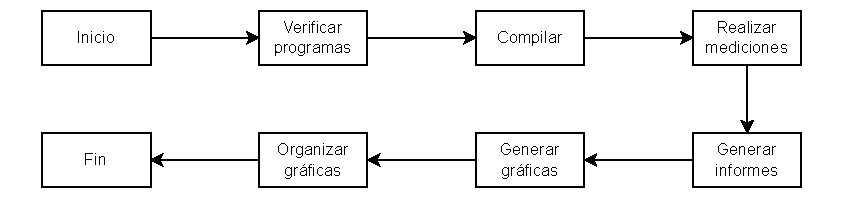
\includegraphics[width=\textwidth]{Pipeline_pro.pdf}
  \caption{Flujo de la pipeline}
  \label{fig:flujo_pipeline}
\end{figure}

\section{Programas utilizados}

Los programas seleccionados están diseñados para revelar de
forma clara el impacto de las medidas de seguridad y de las
optimizaciones aplicadas. Incluyen operaciones básicas sobre memoria,
uso de funciones estándar susceptibles de fortificación, y estructuras
de control simples. Esta elección permite centrarse en los efectos que
introducen los compiladores y sus configuraciones, sin interferencias
derivadas de la complejidad del código fuente.

\section{Enfoque visual y tipo de gráficas}

Debido a la gran cantidad de combinaciones evaluadas y métricas
recogidas, se ha optado por una presentación gráfica que permita
identificar patrones y diferencias de forma clara. Todas las gráficas
comparan los tres compiladores de manera simultánea y están agrupadas en
función del eje de comparación principal:

\begin{itemize}
\item
  \textbf{Comparación por nivel de optimización} (Figuras \ref{fig:Gráficas_gráficas_por_optimización__o0_file_size_kb} a \ref{fig:Gráficas_gráficas_por_optimización__oz_time_ms}).
  Se fija una medida de seguridad concreta y se comparan diferentes
  niveles de optimización. Permite observar cómo afecta la optimización
  al rendimiento, tamaño o fortificación del binario bajo una misma
  política de seguridad.
\item
  \textbf{Comparación por medida de seguridad} (Figuras \ref{fig:Gráficas_gráficas_por_medida_seguridad_debug_assertions_file_size_kb} a \ref{fig:Gráficas_gráficas_por_medida_seguridad_stack_protection_strong_time_ms}).
  Se fija un nivel de optimización y se comparan distintas \emph{flags}
  de seguridad. Esto permite analizar el impacto relativo de cada
  protección bajo un mismo entorno de rendimiento.
\item
  \textbf{Versión porcentual} (Figuras \ref{fig:Gráficas_gráficas_por_optimización_porcentual__o0_file_size_kb} a \ref{fig:Gráficas_gráficas_por_medida_seguridad_porcentual_stack_protection_strong_time_ms_porcentaje}).
  Además de las comparaciones directas, también se generan versiones en
  las que los resultados se expresan como porcentajes respecto al
  programa base sin optimizaciones ni medidas de seguridad. Esto permite
  ver de forma clara cuánto mejora o empeora cada opción, sin fijarse en
  los valores exactos.
\item
  \textbf{Gráfica radar de cobertura de protecciones} (Figuras \ref{fig:Gráficas_gráficas_cualitativas_comparacion_compiladores} y \ref{fig:Gráficas_gráficas_cualitativas_gráfico_protecciones}).
  Resume qué medidas de seguridad soporta cada compilador. Esta
  representación permite comparar de forma rápida las capacidades de
  cada uno.
\item
  \textbf{Boxplot general} (Figura \ref{fig:Gráficas_boxplot}).
  Muestra cómo varían los resultados entre las diferentes
  configuraciones y ayuda a detectar casos que se comportan de forma muy
  diferente al resto.
\item
  \textbf{Facet grid comparativo} (Figura \ref{fig:Gráficas_facet_grid}).
  Presenta todas las configuraciones como puntos individuales y permite
  ver varias métricas al mismo tiempo. Así, se pueden comparar
  fácilmente los tres compiladores sin separar por tipo de optimización
  o seguridad.
\end{itemize}

Todas estas visualizaciones permiten explorar simultáneamente el efecto
de las configuraciones sobre el tiempo de ejecución, el uso de memoria,
el tamaño del binario y el porcentaje de funciones fortificadas.
En este TFG, el enfoque visual es necesario para interpretar resultados de forma
clara y comprensible, evitando tablas extensas y facilitando la
comparación entre cada compilador.
\chapter{Análisis de resultados}
\label{chap:resultados}

En este capítulo se presentan y analizan los resultados obtenidos de las pruebas realizadas con los compiladores \emph{GCC}, \emph{Clang} y \emph{Rustc}, evaluando el impacto de diferentes niveles de optimización y medidas de seguridad en cuatro métricas: tiempo de ejecución, uso de memoria, tamaño del archivo generado y porcentaje de funciones fortificadas. Los experimentos se han llevado a cabo en un entorno controlado utilizando programas específicamente diseñados para aislar los efectos de las combinaciones evaluadas. El análisis comparativo revela interesantes compensaciones entre rendimiento y seguridad, destacando las fortalezas particulares de cada compilador en diferentes escenarios.

\section{Entorno de experimentación}

Las pruebas se han llevado a cabo en un entorno controlado, utilizando
un único ordenador para asegurar la coherencia de los resultados. A
continuación se detallan las características principales del ordenador
donde se han realizado las pruebas:

\begin{itemize}
\item
  \textbf{Procesador}: Intel Core i7-10750H (6 núcleos físicos, 12
  hilos) con frecuencia base de 2.60\,GHz y turbo de hasta 5.00\,GHz
\item
  \textbf{Memoria RAM}: 16\,GB
\item
  \textbf{Tarjeta gráfica}: NVIDIA GeForce RTX 3060 Mobile / Max-Q
\item
  \textbf{Sistema operativo}: Kali GNU/Linux Rolling (x86\_64)
\item
  \textbf{Kernel}: Linux 6.12.25
\end{itemize}

Para realizar las pruebas se emplearon las siguientes versiones de
compiladores:

\begin{itemize}
\item
  \emph{GCC}: versión 14.2.0 (Debian 14.2.0-19)
\item
  \emph{Clang}: versión 19.1.7 (Debian)
\item
  \emph{Rustc}: versión 1.89.0-nightly
\end{itemize}

La elección de la versión nightly de \emph{Rustc} es debido a que las
opciones avanzadas de seguridad, como los sanitizadores
(\texttt{-Z\ sanitizer=...}) y los protectores de pila
(\texttt{-Z\ stack-protector=...}) no están disponibles en la rama
estable.

\section{Descripción de conjuntos de datos}

Para realizar las pruebas se han utilizado dos programas escritos en C++
y sus equivalentes en Rust. Estos programas han sido diseñados para
activar de forma controlada las protecciones de seguridad evaluadas, y
para generar un nivel de trabajo suficiente como para observar el efecto
de las optimizaciones.


Programa \underline{\textbf{suma.cpp}} / \underline{\textbf{suma.rs}}.
Este programa realiza una operación intensiva sobre un vector de tamaño
considerable (1 millón de posiciones), inicializado con un valor
constante.

En ambos casos, el programa permite observar el impacto de la optimización
sobre bucles y uso de estructuras (\texttt{std::vector} en C++, \texttt{Vec} en Rust), 
los efectos sobre el uso de memoria y el tamaño del binario, y la activación de protecciones
básicas sin provocar errores.\\

Programa \underline{\textbf{final.cpp}} / \underline{\textbf{final.rs}}.
Este programa está específicamente diseñado para mostrar
vulnerabilidades que pueden ser detectadas por mecanismos como
\emph{AddressSanitizer}, \emph{MemorySanitizer} o
\emph{stack\ protector}. El programa realiza una copia insegura de una cadena de 
entrada fija con tamaño de 47 bytes a un búfer pequeño de 32 bytes, 
lo que produce un desbordamiento de memoria en la pila si 
no se aplican medidas de protección.

Las características más releventase son las siguientes: en C++, el uso de 
\texttt{strcpy} (función insegura) junto con un búfer de 32 bytes 
activa múltiples protecciones. La versión de Rust simula un comportamiento 
similar mediante copia manual sin validación de límites. En ambos casos, se 
incluye uso de memoria dinámica para ampliar el análisis.

\bigskip

Ambos programas son breves y están pensados para aislar el efecto de las
medidas de seguridad y las optimizaciones del compilador, evitando
interferencias provocadas por lógica compleja o dependencias externas.
Esto facilita la interpretación de los resultados, especialmente en
gráficos donde se comparan directamente métricas como el tiempo de
ejecución, el uso de memoria o el porcentaje de funciones fortificadas.


Las versiones fueron compiladas sin modificar para cada compilador
evaluado: \emph{GCC}, \emph{Clang} y \emph{Rustc}. No dependen de
bibliotecas externas más allá de la biblioteca estándar, lo que garantiza la
reproducibilidad del experimento en distintos entornos.

\section{Descripción de experimentos y resultados}

\subsection{Diseño del experimento}

Para cada programa —uno en C++ y su versión equivalente en Rust— se
generan múltiples binarios combinando una única flag de seguridad,
seleccionada de entre un conjunto representativo, y un nivel de optimización,
específico de cada compilador.

Esto da lugar a un conjunto amplio de combinaciones para cada lenguaje y
compilador, que posteriormente se comparan en términos de tiempo de ejecución, 
uso de memoria, tamaño del binario resultante y porcentaje de funciones fortificadas.
Cada experimento se ha ejecutado 10 veces para calcular valores medios.

\subsection{Combinaciones}

A continuación se resumen las \emph{flags} con las que se realizan las
combinaciones evaluadas para cada compilador. Las tablas \ref{tab:gcc_optimizacion},
\ref{tab:clang_optimizacion} y \ref{tab:rust_optimizacion} muestran las opciones de
optimización para cada compilador, mientras que las opciones de seguridad se encuentran en las Tablas
\ref{tab:gcc_seguridad}, \ref{tab:clang_seguridad} y \ref{tab:rust_seguridad}.


\begin{table}[H]
\centering
\small % Tamaño de fuente más pequeño
\begin{tabularx}{\linewidth}{|l|Y|}
\hline
\textbf{\emph{Flag}} & \textbf{Descripción} \\
\hline
\texttt{-O0} & Sin optimización. Compilación rápida, ejecución lenta. \\
\texttt{-O1} & Optimización básica, reduce algo el tamaño y mejora rendimiento. \\
\texttt{-O2} & Optimización estándar, buena relación entre velocidad y tamaño. \\
\texttt{-O3} & Optimización agresiva, busca máximo rendimiento (puede aumentar el tamaño). \\
\texttt{-Os} & Optimiza para reducir el tamaño del binario. \\
\hline
\end{tabularx}
\caption{Niveles de optimización en \emph{GCC} [15]}
\label{tab:gcc_optimizacion}
\end{table}

\begin{table}[H]
\centering
\footnotesize % Tamaño de fuente aún más pequeño para tabla ancha
\begin{tabularx}{\linewidth}{|l|Y|}
\hline
\textbf{\emph{Flag}} & \textbf{Descripción} \\
\hline
\texttt{(vacío)} & Sin protecciones adicionales. \\
\texttt{-no-pie} & Ejecutable con dirección de carga fija (menos seguro). \\
\texttt{-pie} & Ejecutable con dirección de carga aleatoria (\emph{PIE}). \\
\texttt{-D\_FORTIFY\_SOURCE=2} & Fortificación avanzada de funciones inseguras. \\
\texttt{-D\_FORTIFY\_SOURCE=1} & Fortificación básica. \\
\texttt{-U\_FORTIFY\_SOURCE} & Desactiva la fortificación. \\
\texttt{-z noexecstack} & Evita que la memoria de ejecución tenga permiso de ejecución. \\
\texttt{-z execstack} & Permite ejecutar código en memoria (menos seguro). \\
\texttt{-fno-plt} & Desactiva tabla de enlaces indirectos (ligero refuerzo de seguridad). \\
\texttt{-fsanitize=address} & Detecta accesos inválidos a memoria (\emph{AddressSanitizer}). \\
\texttt{-fsanitize=undefined} & Detecta comportamientos indefinidos del lenguaje. \\
\texttt{-Wl,-z,relro,-z,now} & Protege la tabla de enlaces contra sobrescrituras (\emph{Full RELRO}). \\
\texttt{-fno-stack-protector} & Desactiva protección contra desbordamiento de variables locales. \\
\texttt{-fstack-protector} & Protección básica contra desbordamiento de pila. \\
\texttt{-fstack-protector-strong} & Protección más amplia contra desbordamientos. \\
\texttt{-fstack-protector-all} & Protección total: cualquier función con variables en pila será protegida. \\
\hline
\end{tabularx}
\caption{\emph{Flags} de seguridad en \emph{GCC} [16]}
\label{tab:gcc_seguridad}
\end{table}


\begin{table}[H]
\centering
\small
\begin{tabularx}{\linewidth}{|l|Y|}
\hline
\textbf{\emph{Flag}} & \textbf{Descripción} \\
\hline
\texttt{-O0} & Sin optimización. Compilación rápida, ejecución lenta. \\
\texttt{-O1} & Optimización básica, reduce algo el tamaño y mejora rendimiento. \\
\texttt{-O2} & Optimización estándar, buena relación entre velocidad y tamaño. \\
\texttt{-O3} & Optimización agresiva, busca máximo rendimiento (puede aumentar el tamaño). \\
\texttt{-Os} & Optimiza para reducir el tamaño del binario. \\
\texttt{-Oz} & Optimiza para reducir el tamaño del binario al máximo. \\
\texttt{-Ofast} & Optimiza con máxima agresividad, desactiva comprobaciones de precisión numérica. \\
\hline
\end{tabularx}
\caption{Niveles de optimización en \emph{Clang} [17]}
\label{tab:clang_optimizacion}
\end{table}

\begin{table}[H]
\centering
\footnotesize
\begin{tabularx}{\linewidth}{|l|Y|}
\hline
\textbf{\emph{Flag}} & \textbf{Descripción} \\
\hline
\texttt{(vacío)} & Sin protecciones adicionales. \\
\texttt{-fstack-protector} & Igual que en \emph{GCC}. \\
\texttt{-fstack-protector-strong} & Igual que en \emph{GCC}. \\
\texttt{-fstack-protector-all} & Igual que en \emph{GCC}. \\
\texttt{-fno-stack-protector} & Igual que en \emph{GCC}. \\
\texttt{-pie -f\emph{PIE}} & Activa ejecutable independiente de la dirección de carga (\emph{PIE}). \\
\texttt{-no-pie} & Desactiva \emph{PIE}. \\
\texttt{-D\_FORTIFY\_SOURCE=2} & Nivel de fortificación. \\
\texttt{-D\_FORTIFY\_SOURCE=1} & Nivel de fortificación. \\
\texttt{-D\_FORTIFY\_SOURCE=0} & Desactivación. \\
\texttt{-z noexecstack} & Evita que la memoria de ejecución tenga permiso de ejecución. \\
\texttt{-Wl,-z,execstack} & Permite ejecutar código en memoria (menos seguro). \\
\texttt{-fno-plt} & Desactiva la tabla de enlaces indirectos. \\
\texttt{-fsanitize=address} & Sanitizadores para errores de memoria. \\
\texttt{-fsanitize=undefined} & Sanitizadores para comportamiento indefinido. \\
\texttt{-Wl,-z,relro,-z,now} & Protege estructuras internas al enlazar ficheros (\emph{Full RELRO}). \\
\texttt{-flto} & Activación de optimization al enlazar ficheros (global entre archivos). \\
\texttt{-fsanitize=safe-stack} & Protección específica: separa datos vulnerables de otras variables en pila. \\
\texttt{-fsanitize=memory} & Detecta uso de memoria sin inicializar (\emph{MemorySanitizer}). \\
\hline
\end{tabularx}
\caption{\emph{Flags} de seguridad en \emph{Clang} [17]}
\label{tab:clang_seguridad}
\end{table}


\begin{table}[H]
\centering
\small
\begin{tabularx}{\linewidth}{|l|Y|}
\hline
\textbf{\emph{Flag}} & \textbf{Descripción} \\
\hline
\texttt{-C opt-level=0} & Sin optimización. \\
\texttt{-C opt-level=1} & Optimización básica. \\
\texttt{-C opt-level=2} & Optimización estándar. \\
\texttt{-C opt-level=3} & Optimización máxima. \\
\texttt{-C opt-level=s} & Optimiza para tamaño reducido. \\
\texttt{-C opt-level=z} & Optimiza para tamaño mínimo absoluto. \\
\hline
\end{tabularx}
\caption{Niveles de optimización en \emph{Rustc} [18]}
\label{tab:rust_optimizacion}
\end{table}

\begin{table}[H]
\centering
\footnotesize
\begin{tabularx}{\linewidth}{|l|Y|}
\hline
\textbf{\emph{Flag}} & \textbf{Descripción} \\
\hline
\texttt{(vacío)} & Sin medidas adicionales. \\
\texttt{-C overflow-checks=on} & Comprobación en tiempo de ejecución de desbordamientos aritméticos. \\
\texttt{-C debug-assertions=on} & Comprobaciones de depuración activadas. \\
\texttt{-C panic=abort} & El programa se aborta directamente ante un error grave (más rápido, menos seguro). \\
\texttt{-C lto} & Optimization al enlazar ficheros (convencional). \\
\texttt{-C lto=thin} & Optimization al enlazar ficheros (más ligera). \\
\texttt{-Z sanitizer=address} & Detecta accesos inválidos a memoria (\emph{AddressSanitizer}). \\
\texttt{-Z sanitizer=leak} & Detecta fugas de memoria (\emph{LeakSanitizer}). \\
\texttt{-Z sanitizer=memory} & Detecta uso de memoria sin inicializar (\emph{MemorySanitizer}). \\
\texttt{-C link-arg=-Wl,-z,relro,-z,now} & Protege estructuras internas al enlazar (\emph{Full RELRO}). \\
\texttt{-Z stack-protector=strong} & Protección fuerte contra desbordamientos. \\
\texttt{-Z stack-protector=basic} & Protección básica de pila. \\
\texttt{-Z stack-protector=none} & Sin protección de pila. \\
\texttt{-C link-arg=-Wl,-z,noexecstack} & Memoria no ejecutable. \\
\texttt{-C link-arg=-Wl,-z,execstack} & Memoria ejecutable. \\
\texttt{-C relocation-model=pic -C link-arg=-pie} & \emph{PIE} habilitado. \\
\texttt{-C relocation-model=static -C link-arg=-no-pie} & \emph{PIE} deshabilitado. \\
\hline
\end{tabularx}
\caption{\emph{Flags} de seguridad en \emph{Rustc} [19]}
\label{tab:rust_seguridad}
\end{table}

\section{Análisis de resultados}
Para los resultados se usan medias de varias pruebas realizadas con los distintos programas.

\subsection{Tiempo de ejecución}

\subsubsection{Impacto de las Optimizaciones (\texttt{-O0} a \texttt{-Ofast})}
En la Tabla \ref{tab:optimizaciones_por_compilador} se presentan los tiempos de ejecución de los programas sin aplicar ninguna medida de protección. Esto permite establecer una línea base para cada nivel de optimización, con el objetivo de compararlos posteriormente con los tiempos obtenidos al activar medidas de seguridad y así evaluar el impacto que estas tienen en cada nivel de optimización. Además, se busca analizar la mejora relativa entre los distintos niveles de optimización para entender mejor cómo influyen dichas medidas en relación con el comportamiento del archivo base.


\begin{table}[H]
\centering
\footnotesize
\begin{tabular}{|c|c|c|c|}
\hline
\textbf{Nivel} & \textbf{\emph{Clang}} & \textbf{\emph{GCC}} & \textbf{\emph{Rustc}} \\
\hline
\texttt{-O0}    & 1.34 ms         & 1.40 ms        & 1.66 ms        \\
\texttt{-O1}    & 1.33 ms (-0.7\%) & 1.74 ms (+24\%) & 1.35 ms (-19\%) \\
\texttt{-O2}    & 1.55 ms (+16\%)  & 1.08 ms (-23\%) & 2.32 ms (+40\%) \\
\texttt{-O3}    & 1.31 ms (-2\%)   & 1.23 ms (-12\%) & 1.52 ms (-8\%)  \\
\texttt{-Os}    & 1.74 ms (+30\%)  & 1.12 ms (-20\%) & 1.35 ms (-19\%) \\
\texttt{-Oz}    & 2.00 ms (+49\%)  & N/A         & 1.53 ms (-8\%)  \\
\texttt{-Ofast} & 1.34 ms (=)      & N/A         & N/A          \\
\hline
\end{tabular}
\caption{Impacto de las optimizaciones por compilador}
\label{tab:optimizaciones_por_compilador}
\end{table}

En el nivel sin optimización (\texttt{-O0}), \emph{Clang} registra un tiempo de 1.34 ms, \emph{GCC} es ligeramente más lento con 1.40 ms, y \emph{Rustc} resulta aproximadamente un 24\% más lento que \emph{Clang} debido a las verificaciones de seguridad integradas. Al aplicar la optimización \texttt{-O1}, \emph{Clang} mantiene un rendimiento estable con una ligera mejora, \emph{GCC} sufre un retroceso notable y \emph{Rustc} mejora significativamente, superando a \emph{GCC}, lo que indica una mejor optimización en este nivel. Con \texttt{-O2}, \emph{GCC} destaca con la mejor mejora en velocidad, mientras que \emph{Clang} empeora y \emph{Rustc} se penaliza por los checks adicionales que realiza. En \texttt{-O3}, \emph{Clang} y \emph{GCC} alcanzan tiempos cercanos, con mejoras respecto a niveles previos, mientras que \emph{Rustc} se recupera, aunque sigue siendo el más lento. Al usar la optimización para tamaño \texttt{-Os}, \emph{GCC} ofrece un buen equilibrio con una mejora considerable, mientras \emph{Clang} empeora y \emph{Rustc} mantiene un rendimiento aceptable. En \texttt{-Oz}, \emph{Clang} sacrifica velocidad por un tamaño más reducido, \emph{Rustc} mantiene un rendimiento similar a \texttt{-O3}, y no hay datos disponibles para \emph{GCC}. Finalmente, \texttt{-Ofast}, disponible solo para \emph{Clang}, mantiene un rendimiento similar al nivel sin optimización pero omite comprobaciones de seguridad para maximizar la velocidad. En resumen, \emph{GCC} presenta el mejor rendimiento en niveles como \texttt{-O2} y \texttt{-Os}, \emph{Clang} es consistente y rápido en general, especialmente con \texttt{-Ofast}, y \emph{Rustc}, aunque generalmente más lento, mejora significativamente en ciertos niveles pese a sus medidas de seguridad.


\subsubsection{Impacto de las medidas de seguridad}

El objetivo es calcular el impacto exacto que implica activar protecciones de seguridad en aquellas combinaciones donde se observaron los peores resultados de rendimiento. Para ello, se evalúa el impacto de las \emph{flags} de seguridad en cada compilador utilizando su nivel de optimización óptimo, determinado según los datos de rendimiento previamente analizados: en el caso de \emph{Clang}, se selecciona \texttt{-O3} por su rendimiento consistente; para \emph{GCC}, se opta por \texttt{-O3}, ya que fue el mejor tiempo en las pruebas; y para \emph{Rustc}, se utiliza también \texttt{-O3}, al ofrecer un buen equilibrio entre seguridad y rendimiento. Los datos extraídos de las pruebas pueden consultarse en las Figuras \ref{fig:Gráficas_gráficas_por_optimización__o2_time_ms} y \ref{fig:Gráficas_gráficas_por_optimización__o3_time_ms}.

\begin{table}[H]
\centering
\footnotesize
\begin{tabular}{|l|c|c|c|}
\hline
\emph{\textbf{Flag}} & \textbf{\emph{Clang} (\texttt{-O3})} & \textbf{\emph{GCC} (\texttt{-O3})} & \textbf{\emph{Rustc} (\texttt{-O3})}\\
\hline
\texttt{-fstack-protector-strong} & 1.31 $\rightarrow$ 1.35 ms & 1.08 $\rightarrow$ 1.65 ms & 1.52 $\rightarrow$ 1.39 ms\\
\texttt{-D\_FORTIFY\_SOURCE=2} (C/C++) & 1.31 $\rightarrow$ 1.23 ms & 1.08 $\rightarrow$ 1.23 ms & N/A\\
\hline
\multicolumn{4}{|l|}{\textbf{Sanitizadores:}} \\
\hline
\texttt{-fsanitize=address} & 1.31 $\rightarrow$ 1.46 ms & 1.08 $\rightarrow$ 1.78 ms & 1.52 $\rightarrow$ 2.40 ms\\
\texttt{-Z sanitizer=memory} (Rust) & N/A & N/A & 1.52 $\rightarrow$ 2.71 ms\\
\hline
\end{tabular}
\caption{Casos con mayor impacto de flags de seguridad en niveles óptimos}
\label{tab:overhead_optimos}
\end{table}

Tras las pruebas y observando los peores resultados, se han resumido en la Tabla \ref{tab:overhead_optimos} los casos donde las \emph{flags} de seguridad causan el mayor impacto en el rendimiento para cada compilador en su nivel óptimo de optimización (\texttt{-O3}). Como se puede observar, \emph{GCC} presenta el mayor incremento relativo de tiempo de ejecución al activar ciertas protecciones, especialmente con el uso del \texttt{-fstack-protector-strong}. Por otro lado, \emph{Rustc} mantiene un coste relativamente bajo al emplear las \emph{flags} estándar, como las verificaciones de desbordamiento (\emph{overflow checks}), aunque los sanitizadores como el \texttt{-Z sanitizer=memory} aumentan significativamente el tiempo de ejecución. \emph{Clang} muestra un comportamiento intermedio, con un impacto moderado al activar estas protecciones.

\subsubsection{Comparativa final: seguridad vs. rendimiento}

En la Tabla \ref{tab:seguridad_vs_rendimiento} se ha elegido un nivel típico para producción como \texttt{-O3}
y se han comparado los tiempos de ejecución de cada compilador sin \emph{flags} de seguridad junto al impacto
que suponen aquellas comunes en este ámbito como \texttt{-fstack-protector-strong} y \texttt{-D\_FORTIFY\_SOURCE=2}.

\begin{table}[H]
\centering
\footnotesize
\begin{tabular}{|c|c|c|l|}
\hline
\textbf{Compilador} & \textbf{Tiempo (ms)} & \textbf{Impacto seguridad} & \textbf{Ventaja principal} \\
\hline
\emph{Clang} & 1.55 & -1.53\% (con \emph{flags}) & Optimización estable. \\
\emph{GCC}     & 1.08 & +33.34\% (con \emph{flags}) & Mejor rendimiento en \texttt{-O3}. \\
\emph{Rustc}   & 2.32 & -8.55\% (con \emph{flags}) & Seguridad sin configurar. \\
\hline
\end{tabular}
\caption{Comparativa de seguridad vs rendimiento}
\label{tab:seguridad_vs_rendimiento}
\end{table}

\subsubsection{Conclusiones}

En código con alta demanda de rendimiento la opción recomendada es\\
\emph{Clang}\ \texttt{-O3}\ \texttt{-D\_FORTIFY\_SOURCE=2\ -fstack-protector-strong}.
Aunque sufre un impacto combinado que reduce el tiempo en un 1.53\,\%,
siendo el más rápido. Esta opción se considera la ideal para entornos donde se
prioriza el rendimiento pero se requiere cierta protección básica.
En \emph{GCC}\ se debe evitar \texttt{-O3}\ \texttt{-D\_FORTIFY\_SOURCE=2\ -fstack-protector-strong}
ya que su tiempo aumenta en un 33.34.

En código donde la seguridad es crítica la mejor opción es
\emph{Rustc}\ \texttt{-O3} ya que mantiene un excelente equilibrio, posee
seguridad por defecto, y puede llegar a reducirse en 8.55\,\% el tiempo al
sumar protecciones. Además, no requiere configuración adicional para la
mayoría de los checks (desbordamiento, acceso inválido, etcétera).

En desarrollo, pruebas y depuración para C/C++, es muy recomendable el uso de
\texttt{-fsanitize=address} junto con los niveles de optimización \texttt{-O1} o \texttt{-O3} para
detectar errores de memoria. Aunque presenta un impacto elevado
($\sim$+64.81\,\%), resulta sumamente útil para capturar fallos complejos y difíciles de reproducir.
En el caso de Rust, la opción
\texttt{-Z\ sanitizer=memory} permite detectar accesos inválidos y condiciones de carrera con un impacto
similar en el rendimiento ($\sim$+78.28\,\%), siendo una herramienta eficaz en entornos de prueba. Estas variaciones
pueden ser observadas en la Figura \ref{fig:Gráficas_gráficas_por_optimización_porcentual__o3_time_ms}.

Los sanitizadores deben evitarse en producción, ya que pueden multiplicar el tiempo de ejecución hasta por 1.8×. 
Rust se destaca por ofrecer protecciones de memoria integradas con un impacto mínimo en el rendimiento, 
lo que lo convierte en una opción sólida cuando la seguridad no es negociable. \emph{GCC}, por otro lado, alcanza 
el mejor rendimiento bruto incluso al aplicar medidas de seguridad, aunque requiere ajustes más precisos y presenta 
un comportamiento menos predecible en niveles de optimización intermedios.

\subsection{Uso de memoria}

\subsection*{Efecto de las optimizaciones}

Las optimizaciones afectan el uso de memoria de manera diferente según el compilador y el nivel aplicado. A continuación, se detalla el consumo exacto en KB en las Tablas \ref{tab:memoria_clang}, \ref{tab:memoria_gcc} y \ref{tab:memoria_rustc} para \emph{Clang}, \emph{GCC} y \emph{Rustc}, respectivamente.

\begin{table}[H]
\centering
\footnotesize
\begin{tabular}{|l|c|c|}
\hline
\textbf{Nivel de optimización} & \textbf{Memoria (KB)} & \textbf{Variación respecto a \texttt{-O0}} \\
\hline
\texttt{-O0} (sin optimización) & 3270 & — \\
\texttt{-O1} & 3446 & \textbf{+5.4\%} \\
\texttt{-O2} & 3489 & \textbf{+6.7\%} \\
\texttt{-O3} & 3433 & \textbf{+5.0\%} \\
\texttt{-Os} (optimizado para tamaño) & 3416 & \textbf{+4.5\%} \\
\texttt{-Oz} (máxima reducción de tamaño) & \textbf{3013} & \textbf{-7.9\%}\\
\texttt{-Ofast} & 3448 & \textbf{+5.4\%} \\
\hline
\end{tabular}
\caption{Uso de memoria en \emph{Clang} según nivel de optimización}
\label{tab:memoria_clang}
\end{table}


\begin{table}[H]
\centering
\footnotesize
\begin{tabular}{|l|c|c|}
\hline
\textbf{Nivel de optimización} & \textbf{Memoria (KB)} & \textbf{Variación respecto a \texttt{-O0}} \\
\hline
\texttt{-O0} & 3052 & — \\
\texttt{-O1} & 3051 & \textbf{-0.03\%}\\
\texttt{-O2} & 3052 & \textbf{0\%} \\
\texttt{-O3} & 3459 & \textbf{+13.3\%}\\
\texttt{-Os} & \textbf{3038} & \textbf{-0.5\%}\\
\hline
\end{tabular}
\caption{Uso de memoria en \emph{GCC} según nivel de optimización}
\label{tab:memoria_gcc}
\end{table}


\begin{table}[H]
\centering
\footnotesize
\begin{tabular}{|l|c|c|}
\hline
\textbf{Nivel de optimización} & \textbf{Memoria (KB)} & \textbf{Variación respecto a \texttt{-O0}} \\
\hline
\texttt{-O0} & \textbf{1919} & — \\
\texttt{-O1} & 1996 & \textbf{+4.0\%} \\
\texttt{-O2} & 2004 & \textbf{+4.4\%} \\
\texttt{-O3} & 1966 & \textbf{+2.4\%} \\
\texttt{-Os} & 2014 & \textbf{+4.9\%} \\
\texttt{-Oz} & 1976 & \textbf{+3.0\%} \\
\hline
\end{tabular}
\caption{Uso de memoria en \emph{Rustc} según nivel de optimización}
\label{tab:memoria_rustc}
\end{table}

En general, las optimizaciones tienden a aumentar ligeramente el uso de memoria en \emph{Clang}, salvo en el caso de \texttt{-Oz}, que consigue una reducción significativa de aproximadamente un 8\%. Por su parte, \emph{GCC} mantiene un consumo estable en los niveles \texttt{-O0}, \texttt{-O1} y \texttt{-O2}; sin embargo, \texttt{-O3} provoca un aumento del 13\% en el uso de memoria, mientras que \texttt{-Os} logra una ligera reducción. Finalmente, \emph{Rustc} destaca por tener, en general, el menor consumo de memoria, con un incremento moderado y controlado de alrededor del 2 a 5\% debido a las optimizaciones, sin presentar cambios bruscos.


En base a los resultados obtenidos, \texttt{-Oz} (\emph{Clang}) y \texttt{-Os} (\emph{GCC}) son los únicos niveles que reducen memoria respecto a \texttt{-O0}. \texttt{-O3} es el que más aumenta memoria en \emph{GCC} (13\%), pero en \emph{Clang} y \emph{Rustc} el impacto es menor ($\sim$5\%). El compilador más consistente y eficiente es \emph{Rustc}, que siempre está por debajo de 2100 KB.

\subsection*{Efecto de las medidas de seguridad}

Algunas protecciones incrementan significativamente el uso de memoria. Los casos más notables incluyen los sanitizadores, que son los mayores consumidores. Por ejemplo, \emph{AddressSanitizer} puede aumentar la memoria en \emph{Clang} desde aproximadamente 3400 KB hasta $\sim$12000--14000 KB (\texttimes3--4). En \emph{Rustc}, el aumento es de $\sim$2000 KB a $\sim$8000--10000 KB (\texttimes4--5).

Respecto a las protecciones de pila, usar \texttt{-fstack-protector-strong} aumenta la memoria entre 5 y 10\% en \emph{Clang} y \emph{GCC}. Con \texttt{-fstack-protector-all} el aumento puede llegar al 15--20\%, ambos datos son visibles en las Ficguras \ref{fig:Gráficas_gráficas_por_medida_seguridad_porcentual_stack_protection_strong_memory_usage_kb_porcentaje} y \ref{fig:Gráficas_gráficas_por_medida_seguridad_porcentual_stack_protection_all_memory_usage_kb_porcentaje} respectivamente.

Otras protecciones como PIE tienen un impacto menor (2--5\%) como se puede ver en la Figura \ref{fig:Gráficas_gráficas_por_medida_seguridad_porcentual_pie_enabled_memory_usage_kb_porcentaje}. La opción \texttt{-flto} puede incluso reducir ligeramente el uso de memoria (3--5\%).

Rust tiende a manejar mejor ciertas protecciones como el stack protector (aumentos de 5--10\%), mientras que en C++ se elevan más (15--20\%). \emph{Clang} y \emph{GCC} muestran comportamientos similares, aunque \emph{GCC} suele ser ligeramente más eficiente al aplicar sanitizers.

\subsection*{Comparación entre compiladores}

Para estas comparaciones se han utilizado el consumo obtenido en \texttt{-O0} y \texttt{-O3} sin \emph{flags} de seguridad en la Tabla \ref{tab:compiladores_sin_prote} para ver como varía en función del grado de optimización, también se ha hecho la comparativa con algunas protecciones intensivas como \emph{AddressSanitizer}, mostrada en la Tabla \ref{tab:memoria_intensiva}.

\begin{table}[H]
\centering
\footnotesize
\begin{tabular}{|c|c|c|}
\hline
\textbf{Compilador} & \textbf{\texttt{-O0} (KB)} & \textbf{\texttt{-O3} (KB)} \\
\hline
\emph{Clang} & 3270 & 3433 \\
\emph{GCC} & 3052 & 3459 \\
\emph{Rustc} & \textbf{1919} & \textbf{1966} \\
\hline
\end{tabular}
\caption{Consumo en memoria comparado entre compiladores sin protecciones}
\label{tab:compiladores_sin_prote}
\end{table}

\begin{table}[H]
\centering
\footnotesize
\begin{tabular}{|c|c|c|}
\hline
\textbf{Compilador} & \textbf{Memoria base (KB)} & \textbf{Con ASan (KB)} \\
\hline
\emph{GCC} & $\sim$3050 & $\sim$11000--13000 \\
\emph{Clang} & $\sim$3400 & $\sim$12000--14000 \\
\emph{Rustc} & $\sim$2000 & $\sim$8000--10000 \\
\hline
\end{tabular}
\caption{Impacto de \emph{AddressSanitizer} en el uso de memoria}
\label{tab:memoria_intensiva}
\end{table}


\textbf{Optimización para tamaño (\texttt{-Os} / \texttt{-Oz}):}

En cuanto al uso de memoria, \emph{Clang} con la opción \texttt{-Oz} obtuvo un consumo de 3013 KB, siendo este el mejor resultado entre los compiladores de C++. Por su parte \emph{GCC}, usando \texttt{-Os}, presentó un uso ligeramente superior, con 3038 KB. Finalmente, \emph{Rustc} con \texttt{-Oz} demostró ser el más eficiente en términos absolutos, con un consumo de memoria de tan solo 1976 KB como se puede ver en las Figuras \ref{fig:Gráficas_gráficas_por_optimización__os_memory_usage_kb} y \ref{fig:Gráficas_gráficas_por_optimización__oz_memory_usage_kb}.

\subsection*{Conclusión final}

Rust es el más eficiente en cuanto al uso de memoria en todos los escenarios analizados, mostrando un consumo estable incluso al aplicar distintas medidas de seguridad. Por su parte, \emph{Clang} y \emph{GCC} presentan comportamientos comparables, aunque \emph{Clang} logra un mejor rendimiento cuando se compila con la opción \texttt{-Oz} orientada a reducir el tamaño.

Las protecciones que generan un mayor impacto en el uso de memoria son los sanitizadores, ya que pueden multiplicar el consumo por un factor de 3 a 5 veces. En cuanto a las optimizaciones, la opción \texttt{-O3} no siempre mejora el uso de memoria: en \emph{GCC}, por ejemplo, puede incrementar el consumo en un 13\%, mientras que en \emph{Rustc} su efecto es mucho más limitado, con un aumento cercano al 2\%.

\subsection{Tamaño del binario}

\subsubsection{\texorpdfstring{\textbf{Optimización}}{Optimización}}

Las opciones de compilación como \texttt{-Os} y \texttt{-Oz} están
diseñadas para reducir el tamaño de los archivos binarios que se generan
al compilar un programa.
Según los datos analizados, estas opciones logran binarios más pequeños
que los niveles de optimización estándar como \texttt{-O0}, \texttt{-O1}
o \texttt{-O2}. Entre ellas, \texttt{-Oz} es más efectiva en esta tarea
que \texttt{-Os}, ya que logra tamaños incluso menores en algunos casos,
con diferencias que pueden llegar hasta los 6000 KB, como se puede ver
en las Figuras \ref{fig:Gráficas_gráficas_por_optimización__os_file_size_kb} y 
\ref{fig:Gráficas_gráficas_por_optimización__oz_file_size_kb}.

Por otro lado, la opción \texttt{-Ofast} (véase la Figura 
\ref{fig:Gráficas_gráficas_por_optimización__ofast_file_size_kb}), aunque no está disponible en
todos los compiladores, produce binarios más pequeños que los generados
con \texttt{-O3}, pero siguen siendo más grandes que los de \texttt{-Os}
o \texttt{-Oz}, ya que está enfocada en la velocidad de ejecución y no
tanto en el tamaño, aunque algunas optimizaciones ayudan a eliminar
código innecesario.

En cuanto a los niveles más agresivos como \texttt{-O3} y
\texttt{-Ofast}, se observa que generan binarios considerablemente más
grandes, especialmente con \emph{Clang} y \emph{GCC}, debido a
técnicas como la inserción masiva de funciones (\emph{inlining}) y la
vectorización del código.

Aunque \texttt{-Ofast} puede resultar en un tamaño ligeramente menor que
\texttt{-O3}, sigue teniendo un tamaño mayor que las opciones enfocadas
en reducir el tamaño como \texttt{-Os}.

\subsubsection{\texorpdfstring{\textbf{Seguridad}}{Seguridad}}

Cuando se activan ciertas protecciones en la compilación de programas,
el tamaño de los binarios puede aumentar notablemente, tal como muestran
las Figuras \ref{fig:Gráficas_gráficas_por_optimización_porcentual__os_file_size_kb} y
\ref{fig:Gráficas_gráficas_por_optimización_porcentual__oz_file_size_kb}.

Por ejemplo, los sanitizadores como \emph{AddressSanitizer} o \emph{MemorySanitizer}
pueden hacer que el binario final sea entre dos y tres veces más grande
debido a que se añade código adicional para revisar que no haya errores
mientras el programa se está ejecutando.

Otras protecciones como los \emph{stack protectors} también incrementan
el tamaño, aunque en menor medida. Además, mecanismos como RELRO
y {PIE} pueden sumar entre un 10\% y 20\% de tamaño adicional,
según el compilador.

El problema se intensifica cuando se combinan varias protecciones
simultáneamente. Por ejemplo, usar sanitizadores junto con protecciones
de pila y PIE puede llevar a que el binario en \emph{Clang}
supere los 5000 KB, comparado con unos 1000 KB que tiene en una
combinación básica sin \emph{flags} de seguridad.

\subsubsection{\texorpdfstring{\textbf{Comparación entre
compiladores}}{Comparación entre Compiladores}}

En general, los programas compilados con Rust suelen ocupar menos
espacio que los generados con compiladores de C++ como \emph{Clang} o
\emph{GCC}, incluso cuando se usan combinaciones similares.

Por ejemplo, la combinación por defecto en Rust produce binarios más
pequeños que la combinación por defecto en C++. Entre los compiladores
de C++, \emph{Clang} tiende a generar archivos ligeramente más
pequeños que \emph{GCC}, sobre todo cuando se usan opciones como
\texttt{-Os} o \texttt{-Oz}, pensadas para reducir el tamaño.

Al aplicar protecciones adicionales como sanitizadores el aumento de
tamaño es más notable en C++, usar el sanitizador de \emph{Address}
puede duplicar el tamaño del binario, mientras que en Rust el aumento es
más moderado, alrededor de un 50\%. Y se observa que el peor es \emph{Clang}
con hasta un 10000\% de tamaño superior, lo cual se sale mucho de la media.

En cuanto a otras protecciones como RELRO o protecciones de pila,
su efecto sobre el tamaño es similar en todos los compiladores, sin
embargo Rust parece integrar estas medidas de forma más eficiente, ya
que los binarios que genera son menores en tamaño que los de C++.

\subsubsection{\texorpdfstring{\textbf{Recomendaciones}}{Recomendaciones}}

Si lo que se quiere es reducir al máximo el tamaño de un programa, lo
más efectivo es compilarlo con la opción \texttt{-Oz} o \texttt{-Os}. Estas opciones le indican al
compilador que priorice el tamaño del ejecutable por encima del
rendimiento, lo que ayuda a que el resultado final ocupe lo menos
posible. También conviene desactivar herramientas de depuración o
protecciones adicionales que no sean estrictamente necesarias, ya que
suelen aumentar el tamaño del binario.

Ahora bien, si se busca un equilibrio entre tamaño y seguridad, una
buena opción es usar \texttt{-Os} combinado con medidas de protección
como \texttt{-fstack-protector-strong}. A esto se le pueden añadir opciones al enlazador como
\texttt{-Wl,-z,relro,-z,now}, que activan protecciones en tiempo de
ejecución para dificultar la modificación de partes sensibles del
programa.

Por último, no es recomendable usar muchas medidas pesadas al mismo
tiempo como los sanitizadores, PIE o protecciones muy
estrictas para la pila a no ser que sea realmente necesario. Este tipo
de combinaciones puede hacer que el programa aumente bastante de tamaño
y también que tarde más en ejecutarse.

\subsection{Funciones fortificadas}

Una de las principales herramientas para aumentar la seguridad del
código en C y C++ es la opción \texttt{FORTIFY\_SOURCE} [13]. Estas opciones
provocan que el compilador inserte
comprobaciones adicionales en ciertas funciones estándar que podrían ser
un vector de ataque, como los errores de desbordamiento de búfer. En
cambio, el compilador de Rust no admite esta opción, lo que se refleja
en los archivos analizados como ``N/A''.

Los sanitizadores, pese a que su propósito principal no es la
fortificación de funciones, contribuyen a la seguridad detectando
errores de memoria y comportamiento indefinido durante la ejecución del
programa.

La mejor combinación de medidas observada para maximizar la
fortificación es usar \texttt{-D\_FORTIFY\_SOURCE=2} junto con
sanitizadores a partir del nivel \texttt{-O1}, como se muestra en la Figura 
\ref{fig:Gráficas_gráficas_por_optimización__o1_file_size_kb}. 
Este tipo de combinaciones son las que provocan un mayor
porcentaje de funciones protegidas frente a errores, en comparación con
usar \texttt{FORTIFY\_SOURCE=1} por sí solo.
Pese a que Rust no implementa \texttt{FORTIFY\_SOURCE}, sus
sanitizadores pueden añadir una capa adicional de seguridad,
complementando el modelo de seguridad del lenguaje.
Por parte de \emph{GCC} y \emph{Clang}, soportan tanto
\texttt{FORTIFY\_SOURCE} como los sanitizadores. No se observan
diferencias notables en la cantidad de funciones fortificadas cuando se
usan las mismas opciones.

Para finalizar es necesario comentar que aunque Rust no posea soporte para
\texttt{FORTIFY\_SOURCE}, esto no implica menor seguridad.
El lenguaje está diseñado para prevenir errores comunes de memoria
mediante su sistema de tipos y el modelo de \emph{ownership} (gestión de la memoria asignando
un único propietario a cada valor y liberándola automáticamente al finalizar su uso), lo que
reduce la necesidad de fortificación adicional.

Por otro lado, las opciones de optimización como \texttt{-Ofast},
\texttt{-Os} o \texttt{-Oz} no influyen directamente en la
fortificación.


\chapter{Trabajo relacionado}
\label{chap:trabajo}

Numerosos trabajos han analizado las técnicas de defensa a nivel de binario, el coste asociado a activarlas y su integración en compiladores modernos como \emph{GCC}, \emph{Clang} o \emph{Rustc}. Este capítulo resume brevemente algunos de los trabajos y herramientas más relevantes, contextualizando el presente trabajo dentro del panorama actual.

Uno de los enfoques más comunes es el análisis del impacto de medidas como protección de la pila, RELRO, PIE o la fortificación de funciones sobre la ejecución de programas en C y C++. Por ejemplo, proyectos como el \emph{Hardening Guide de Debian} [20] o la documentación de Red Hat [21] han explorado las ventajas y limitaciones de estas protecciones, normalmente desde una perspectiva funcional o de seguridad, pero sin cuantificar en detalle su coste en eficiencia.

También existen herramientas académicas y profesionales como BINSEC [23] que permite analizar programas ya compilados (binarios) utilizando técnicas como la ejecución simbólica, que consiste en simular su comportamiento con variables en lugar de valores concretos. Algunos trabajos en entornos como LLVM han implementado marcos de análisis para evaluar cómo las optimizaciones afectan al rendimiento y seguridad del código generado, pero suelen centrarse en contextos más específicos (optimización interprocedimental, protección frente a ataques concretos, etcétera) [22].

En el caso de Rust, algunos estudios han analizado su diseño como lenguaje seguro por defecto, comparándolo con C/C++ en términos de prevención de errores comunes, aunque pocos lo han integrado en estudios comparativos prácticos que midan rendimiento frente a compiladores tradicionales [23]. En este sentido, el presente trabajo aporta una comparación directa y reproducible entre \emph{Rustc} y otros compiladores ampliamente utilizados, evaluando no solo el soporte de medidas de seguridad, sino también su impacto cuantitativo.

En cuanto a la representación de resultados, aunque es habitual encontrar tablas de rendimiento o medidas aisladas en \emph{benchmarks}, la combinación de informes estructurados y visualizaciones gráficas automáticas como la desarrollada en este proyecto no es común en trabajos anteriores. Esto facilita la comprensión global del efecto de cada configuración, al mismo tiempo que permite detectar patrones generales entre compiladores.

\chapter{Conclusiones y trabajo futuro}
\label{chap:conclusiones}

Este trabajo ha permitido analizar y comparar distintas estrategias de compilación enfocadas tanto en el rendimiento como en la seguridad del software. Se ha estudiado el comportamiento de diferentes compiladores y lenguajes, así como el efecto de múltiples combinaciones de opciones de optimización y protección. A partir de los resultados obtenidos, se han identificado configuraciones que ofrecen un equilibrio adecuado entre eficiencia y robustez, así como otras más orientadas a contextos específicos, como entornos de pruebas o aplicaciones críticas desde el punto de vista de la seguridad.

Una de las principales conclusiones es que no existe una configuración única que sea óptima en todos los casos, sino que la elección debe ajustarse a las necesidades y limitaciones del proyecto de software a compilar. Además, se ha dejado en claro la importancia de entender bien las implicaciones de cada opción de compilación, ya que algunas pueden tener un coste elevado en recursos sin aportar mejoras significativas.

Por otro lado, también se ha confirmado que el diseño de ciertos lenguajes modernos ofrece ventajas estructurales en términos de seguridad, lo que puede simplificar el desarrollo de software más fiable sin necesidad de tantas configuraciones externas.

Como continuación del trabajo realizado se plantea ampliar el conjunto de programas utilizados en las pruebas. Aunque los ejemplos empleados han sido suficientes para observar el efecto de las combinaciones evaluadas, la incorporación de programas con un comportamiento más complejo, o incluso de fragmentos de código reales tomados de proyectos de código abierto, permitiría observar el impacto de las medidas en contextos más realistas y variados.

Otra dirección interesante sería la incorporación de nuevos compiladores o lenguajes. En el caso de C++, podría incluirse el compilador de Microsoft o el de Intel, mientras que a nivel de lenguajes, se podría extender el estudio a otros con orientación a la seguridad como Go o Zig, ampliando así el espectro de comparativa más allá de los compiladores tradicionales.

También sería relevante ejecutar los experimentos en otras arquitecturas o sistemas operativos. Hasta ahora, todas las pruebas se han realizado en una única máquina con Linux y arquitectura x86\_64. Repetir el análisis en entornos ARM o en sistemas como Windows o BSD permitiría evaluar la consistencia de los resultados en plataformas distintas.

A nivel metodológico, sería útil mejorar el \emph{pipeline} de pruebas para hacerlo más modular y extensible. También se podrían introducir mecanismos de paralelización o automatización avanzada para reducir los tiempos de ejecución y facilitar la inclusión de nuevas configuraciones.

Por último, integrar el \emph{pipeline} en entornos de integración continua permitiría su uso en contextos de desarrollo real, facilitando evaluaciones automáticas de seguridad y eficiencia tras cada cambio en el código fuente.


\cleardoublepage
\addcontentsline{toc}{chapter}{Bibliografía}
\bibliographystyle{unsrt} %plaindin
\bibliography{Bibliografia}
\nocite{*} 


\cleardoublepage
\addcontentsline{toc}{chapter}{Anexos}
\chapter*{Anexo A}
\label{chap:anexoA}
{\Large \bfseries Tiempo invertido y diagrama de Gantt}

El diagrama de Gantt en la Figura~\ref{fig:diagrama_gantt} refleja las diferentes fases del proyecto y la dedicación en
el tiempo invertidos. Todo comienza con un periodo de investigación donde
se adquieren los conocimientos previos necesarios. Seguidamente, comienza la etapa de diseño e
implementación de la herramienta desarrollada. Finalmente, el periodo de elaboración de la
memoria. Por otro lado, la Tabla~\ref{tab:horas} detalla el tiempo invertido en cada una de estas fases.

\begin{figure}[htbp]
  \centering
  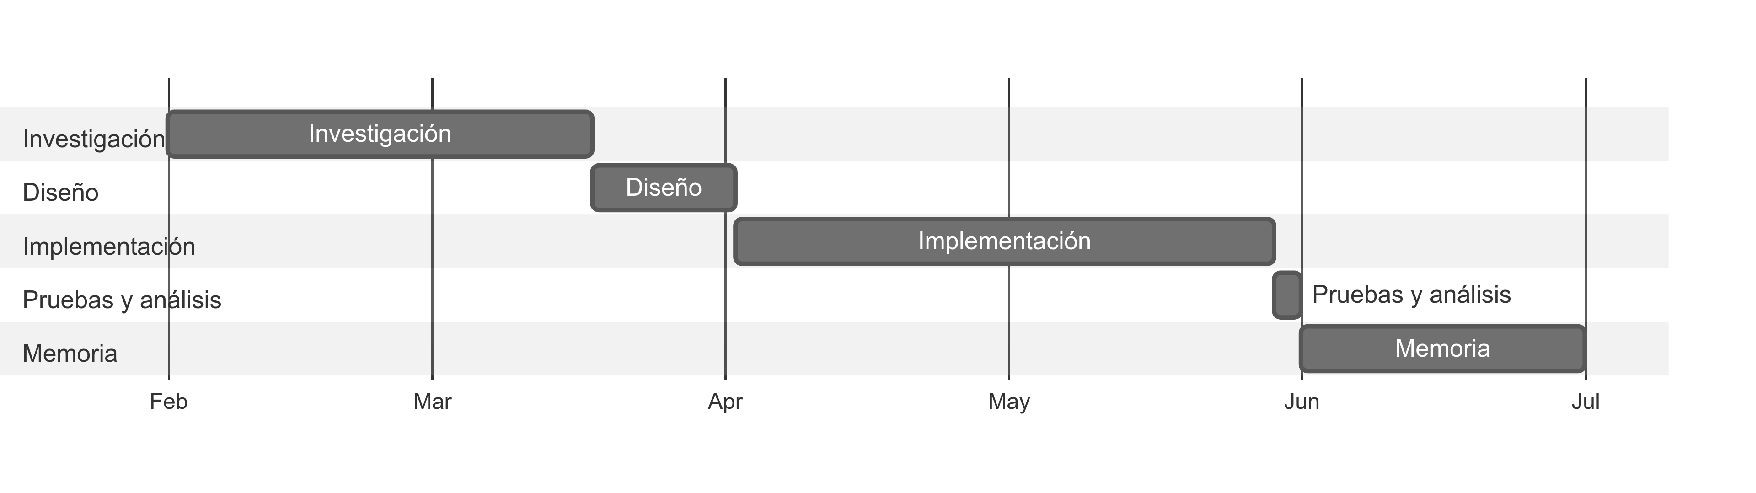
\includegraphics[width=\textwidth]{Diagrama_Gantt.pdf}
  \caption{Diagrama de gantt}
  \label{fig:diagrama_gantt}
\end{figure}

\begin{table}[H]
\centering
\small
\begin{tabular}{|l|r|}
\hline
\textbf{Fase} & \textbf{Horas} \\
\hline
\texttt{Investigación} & 25 \\
\texttt{Diseño} & 40 \\
\texttt{Implementación} & 220 \\
\texttt{Pruebas y análisis} & 20 \\
\texttt{Memoria} & 100 \\
\hline
\texttt{Total} & 405 \\
\hline
\end{tabular}
\caption{Horas invertidas}
\label{tab:horas}
\end{table}
\chapter*{Anexo B}
\label{chap:anexoB}
{\Large \bfseries Gráficas}

Este anexo contiene todas las gráficas generadas durante el análisis.

El color azul corresponde \emph{GCC}, el naranja a \emph{Clang} y el verde a \emph{Rustc}

A continuación las tablas con los valores por defecto de los compiladores, necesario para las gráficas porcentuales.

\begin{table}[H]
\centering
\small % Tamaño de fuente más pequeño
\label{tab:valores_sin_flags}
\begin{tabularx}{\linewidth}{l l >{\centering\arraybackslash}X >{\centering\arraybackslash}X >{\centering\arraybackslash}X >{\centering\arraybackslash}X}
\toprule
\textbf{Compilador} & \textbf{Optimización} & \textbf{Tiempo (ms)} & \textbf{Uso de memoria (KB)} & \textbf{Tamaño del archivo (KB)} & \textbf{Funciones fortificadas (\%)} \\
\midrule
\emph{Clang} & \texttt{-O0} & 1.34 & 3270 & 16.07 & 0.0 \\
 & \texttt{-O1} & 1.33 & 3446 & 16.00 & 0.0 \\
 & \texttt{-O2} & 1.55 & 3489 & 16.00 & 0.0 \\
 & \texttt{-O3} & 1.31 & 3433 & 16.00 & 0.0 \\
 & \texttt{-Os} & 1.74 & 3416 & 16.00 & 0.0 \\
 & \texttt{-Oz} & 2.00 & 3013 & 15.98 & 0.0 \\
 & \texttt{-Ofast} & 1.34 & 3448 & 17.45 & 0.0 \\
\midrule
\emph{GCC} & \texttt{-O0} & 1.40 & 3052 & 16.26 & 0.0 \\
 & \texttt{-O1} & 1.74 & 3051 & 16.04 & 0.0 \\
 & \texttt{-O2} & 1.08 & 3052 & 15.99 & 0.0 \\
 & \texttt{-O3} & 1.23 & 3459 & 16.02 & 0.0 \\
 & \texttt{-Os} & 1.12 & 3038 & 16.04 & 0.0 \\
\midrule
\emph{Rustc} & \texttt{-O0} & 1.66 & 1919 & 3758.80 & 0.0 \\
 & \texttt{-O1} & 1.35 & 1996 & 3752.70 & 0.0 \\
 & \texttt{-O2} & 2.32 & 2004 & 3752.35 & 0.0 \\
 & \texttt{-O3} & 1.52 & 1966 & 3752.35 & 0.0 \\
 & \texttt{-Os} & 1.35 & 2014 & 3752.62 & 0.0 \\
 & \texttt{-Oz} & 1.53 & 1976 & 3752.70 & 0.0 \\
\bottomrule
\end{tabularx}
\caption{Valores por defecto (sin \emph{flags} de seguridad)}
\end{table}

\newpage

\begin{longtable}{l >{\centering\arraybackslash}p{2cm} >{\centering\arraybackslash}p{2cm} >{\centering\arraybackslash}p{2cm} >{\centering\arraybackslash}p{2cm}}
\caption{Valores de referencia y por \emph{flag} de seguridad (optimización \texttt{-O0})} \label{tab:valores_flags} \\
\toprule
\textbf{Configuración} & \textbf{Tiempo (ms)} & \textbf{Uso de memoria (KB)} & \textbf{Tamaño del archivo (KB)} & \textbf{Funciones fortificadas (\%)} \\
\midrule
\endfirsthead

\multicolumn{5}{c}%
{{\tablename\ \thetable{} -- Continuación de la página anterior}} \\
\toprule
\textbf{Configuración} & \textbf{Tiempo (ms)} & \textbf{Uso de memoria (KB)} & \textbf{Tamaño del archivo (KB)} & \textbf{Funciones fortificadas (\%)} \\
\midrule
\endhead

\midrule
\multicolumn{5}{r}{{Continúa en la página siguiente}} \\
\endfoot

\bottomrule
\endlastfoot

\multicolumn{5}{l}{\textbf{Valores por defecto (sin \emph{flags} de seguridad)}} \\
\emph{Clang} & 1.34 & 3270 & 16.07 & 0.0 \\
\emph{GCC} & 1.40 & 3052 & 16.26 & 0.0 \\
\emph{Rustc} & 1.66 & 1919 & 3758.80 & 0.0 \\
\midrule

\multicolumn{5}{l}{\textbf{Stack protector}} \\
\multicolumn{5}{l}{\textit{basic}} \\
\emph{Clang} & 1.66 & 3153 & 16.13 & 0.0 \\
\emph{GCC} & 1.29 & 3182 & 16.32 & 0.0 \\
\emph{Rustc} & 1.90 & 2039 & 3759.80 & 0.0 \\
\multicolumn{5}{l}{\textit{strong}} \\
\emph{Clang} & 2.18 & 3118 & 16.13 & 0.0 \\
\emph{GCC} & 1.29 & 3182 & 16.32 & 0.0 \\
\emph{Rustc} & 1.99 & 1955 & 3759.91 & 0.0 \\
\multicolumn{5}{l}{\textit{all}} \\
\emph{Clang} & 1.66 & 3153 & 16.13 & 0.0 \\
\emph{GCC} & 1.22 & 3188 & 16.32 & 0.0 \\
\emph{Rustc} & N/A & N/A & N/A & N/A \\
\multicolumn{5}{l}{\textit{disabled}} \\
\emph{Clang} & 1.48 & 3322 & 16.07 & 0.0 \\
\emph{GCC} & 1.23 & 3045 & 16.26 & 0.0 \\
\emph{Rustc} & 1.25 & 1968 & 3758.80 & 0.0 \\
\midrule

\multicolumn{5}{l}{\textbf{PIE}} \\
\multicolumn{5}{l}{\textit{enabled}} \\
\emph{Clang} & 1.19 & 3348 & 16.07 & 0.0 \\
\emph{GCC} & 1.06 & 3052 & 16.26 & 0.0 \\
\emph{Rustc} & 1.14 & 1999 & 3758.80 & 0.0 \\
\multicolumn{5}{l}{\textit{disabled}} \\
\emph{Clang} & 1.34 & 3312 & 15.91 & 0.0 \\
\emph{GCC} & 1.46 & 3045 & 16.09 & 0.0 \\
\emph{Rustc} & 1.20 & 1922 & 3740.59 & 0.0 \\
\midrule

\multicolumn{5}{l}{\textbf{Execstack}} \\
\multicolumn{5}{l}{\textit{disabled}} \\
\emph{Clang} & 1.29 & 3310 & 16.07 & 0.0 \\
\emph{GCC} & 2.08 & 3052 & 16.26 & 0.0 \\
\emph{Rustc} & 1.22 & 1886 & 3758.80 & 0.0 \\
\multicolumn{5}{l}{\textit{enabled}} \\
\emph{Clang} & 3.00 & 3322 & 16.07 & 0.0 \\
\emph{GCC} & 1.07 & 3050 & 16.26 & 0.0 \\
\emph{Rustc} & 1.52 & 1960 & 3758.80 & 0.0 \\
\midrule

\multicolumn{5}{l}{\textbf{Sanitizadores}} \\
\multicolumn{5}{l}{\textit{AddressSanitizer}} \\
\emph{Clang} & 2.65 & 13462 & 1660.77 & 15.1 \\
\emph{GCC} & 1.22 & 24964 & 25.92 & 0.0 \\
\emph{Rustc} & 1.75 & 12688 & 6251.03 & 11.5 \\
\multicolumn{5}{l}{\textit{UndefinedSanitizer}} \\
\emph{Clang} & 2.27 & 5600 & 416.24 & 75.0 \\
\emph{GCC} & 1.09 & 3045 & 17.04 & 0.0 \\
\emph{Rustc} & N/A & N/A & N/A & N/A \\
\midrule

\multicolumn{5}{l}{\textbf{Fortify Source}} \\
\multicolumn{5}{l}{\textit{level-2}} \\
\emph{Clang} & 1.52 & 3274 & 16.07 & 0.0 \\
\emph{GCC} & 1.33 & 3052 & 16.26 & 0.0 \\
\emph{Rustc} & N/A & N/A & N/A & N/A \\
\multicolumn{5}{l}{\textit{level-1}} \\
\emph{Clang} & 1.54 & 3342 & 16.07 & 0.0 \\
\emph{GCC} & 1.24 & 3052 & 16.26 & 0.0 \\
\emph{Rustc} & N/A & N/A & N/A & N/A \\
\multicolumn{5}{l}{\textit{disabled}} \\
\emph{Clang} & 1.14 & 3283 & 16.07 & 0.0 \\
\emph{GCC} & 1.15 & 3039 & 16.26 & 0.0 \\
\emph{Rustc} & N/A & N/A & N/A & N/A \\
\midrule

\multicolumn{5}{l}{\textbf{RELRO}} \\
\multicolumn{5}{l}{\textit{full}} \\
\emph{Clang} & 2.70 & 3312 & 15.95 & 0.0 \\
\emph{GCC} & 1.12 & 3052 & 16.14 & 0.0 \\
\emph{Rustc} & 2.29 & 2001 & 3758.80 & 0.0 \\
\midrule

\multicolumn{5}{l}{\textbf{Safe stack}} \\
\multicolumn{5}{l}{\textit{enabled}} \\
\emph{Clang} & 1.34 & 3104 & 22.96 & 20.0 \\
\emph{GCC} & N/A & N/A & N/A & N/A \\
\emph{Rustc} & N/A & N/A & N/A & N/A \\
\midrule

\multicolumn{5}{l}{\textbf{Overflow checks}} \\
\multicolumn{5}{l}{\textit{enabled}} \\
\emph{Clang} & N/A & N/A & N/A & N/A \\
\emph{GCC} & N/A & N/A & N/A & N/A \\
\emph{Rustc} & 1.40 & 1962 & 3758.80 & 0.0 \\
\midrule

\multicolumn{5}{l}{\textbf{Debug assertions}} \\
\multicolumn{5}{l}{\textit{enabled}} \\
\emph{Clang} & N/A & N/A & N/A & N/A \\
\emph{GCC} & N/A & N/A & N/A & N/A \\
\emph{Rustc} & 1.25 & 1984 & 3758.80 & 0.0 \\
\midrule

\multicolumn{5}{l}{\textbf{Panic}} \\
\multicolumn{5}{l}{\textit{abort}} \\
\emph{Clang} & N/A & N/A & N/A & N/A \\
\emph{GCC} & N/A & N/A & N/A & N/A \\
\emph{Rustc} & 1.42 & 1996 & 3752.00 & 0.0 \\
\end{longtable}

\newpage

% Auto-generated LaTeX file with all figures
% This file was automatically generated by a Python script


% === Boxplot ===
\subsection*{Boxplot}
\begin{figure}[htbp]
  \centering
  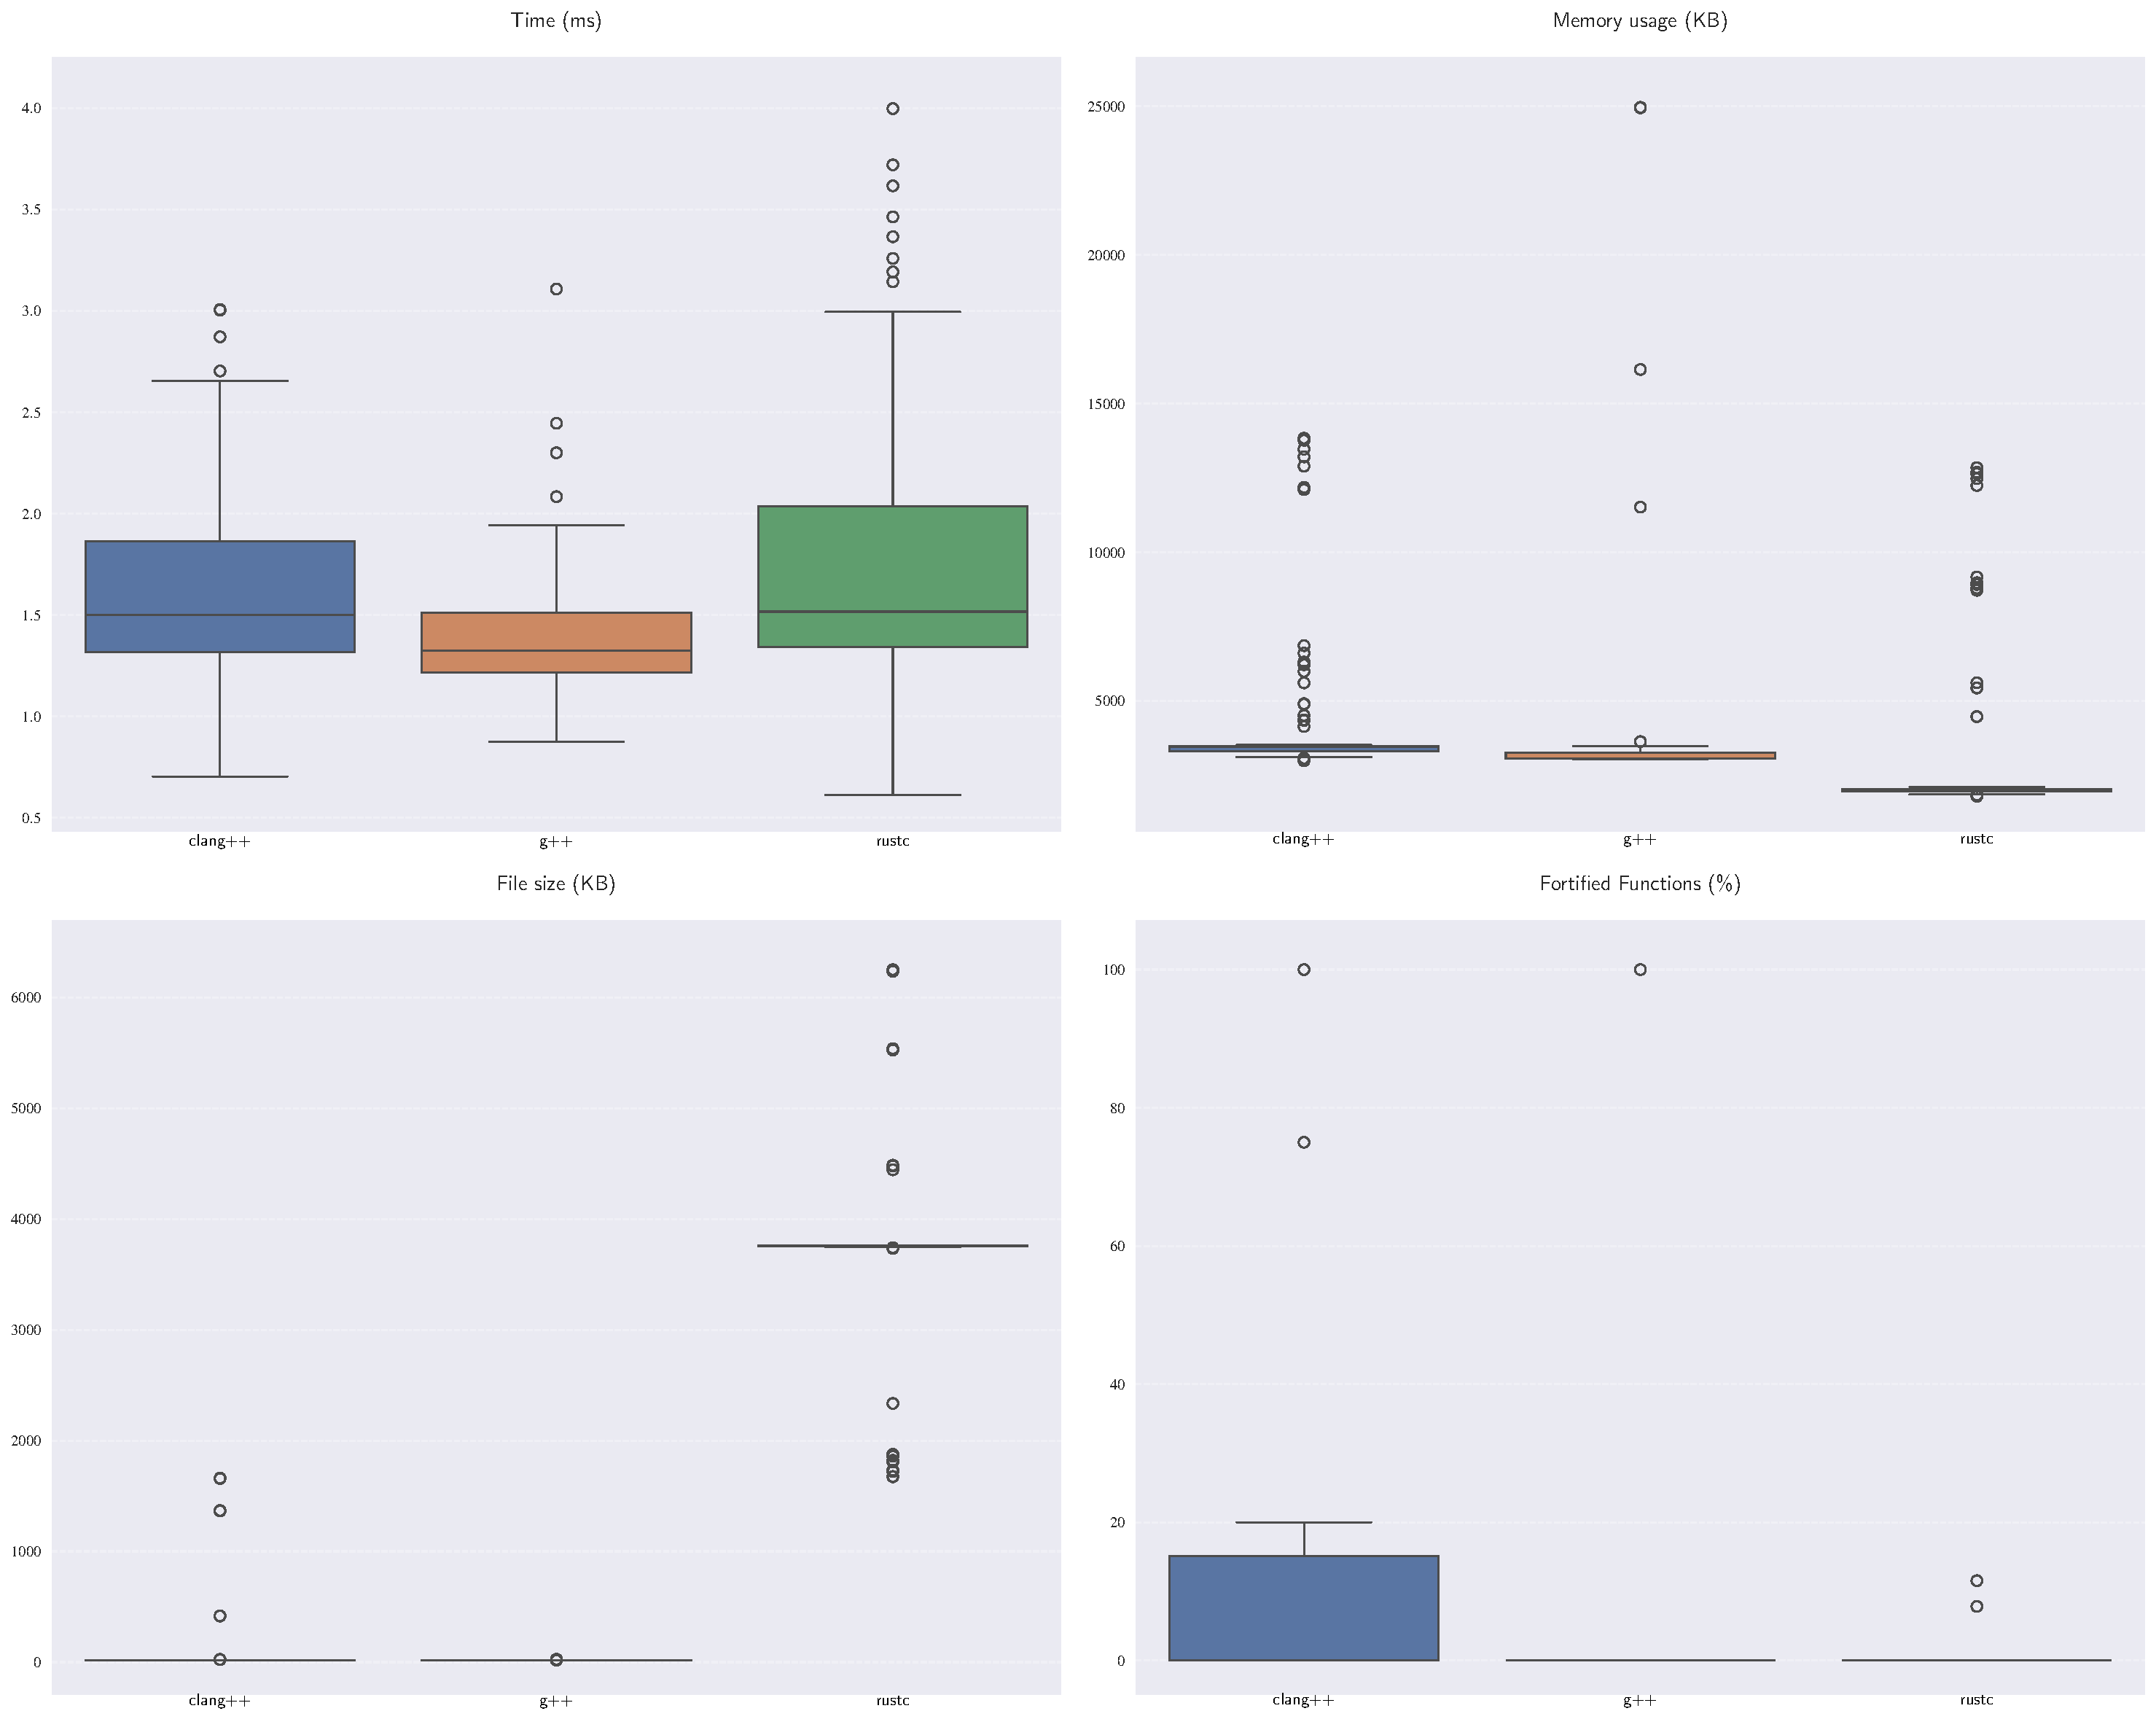
\includegraphics[width=\textwidth, height=0.85\textheight, keepaspectratio]{Gráficas/./Boxplot.pdf}
  \caption{Boxplot}
  \label{fig:Gráficas_boxplot}
\end{figure}
\newpage

% === Facet_Grid ===
\subsection*{Facet Grid}
\begin{figure}[htbp]
  \centering
  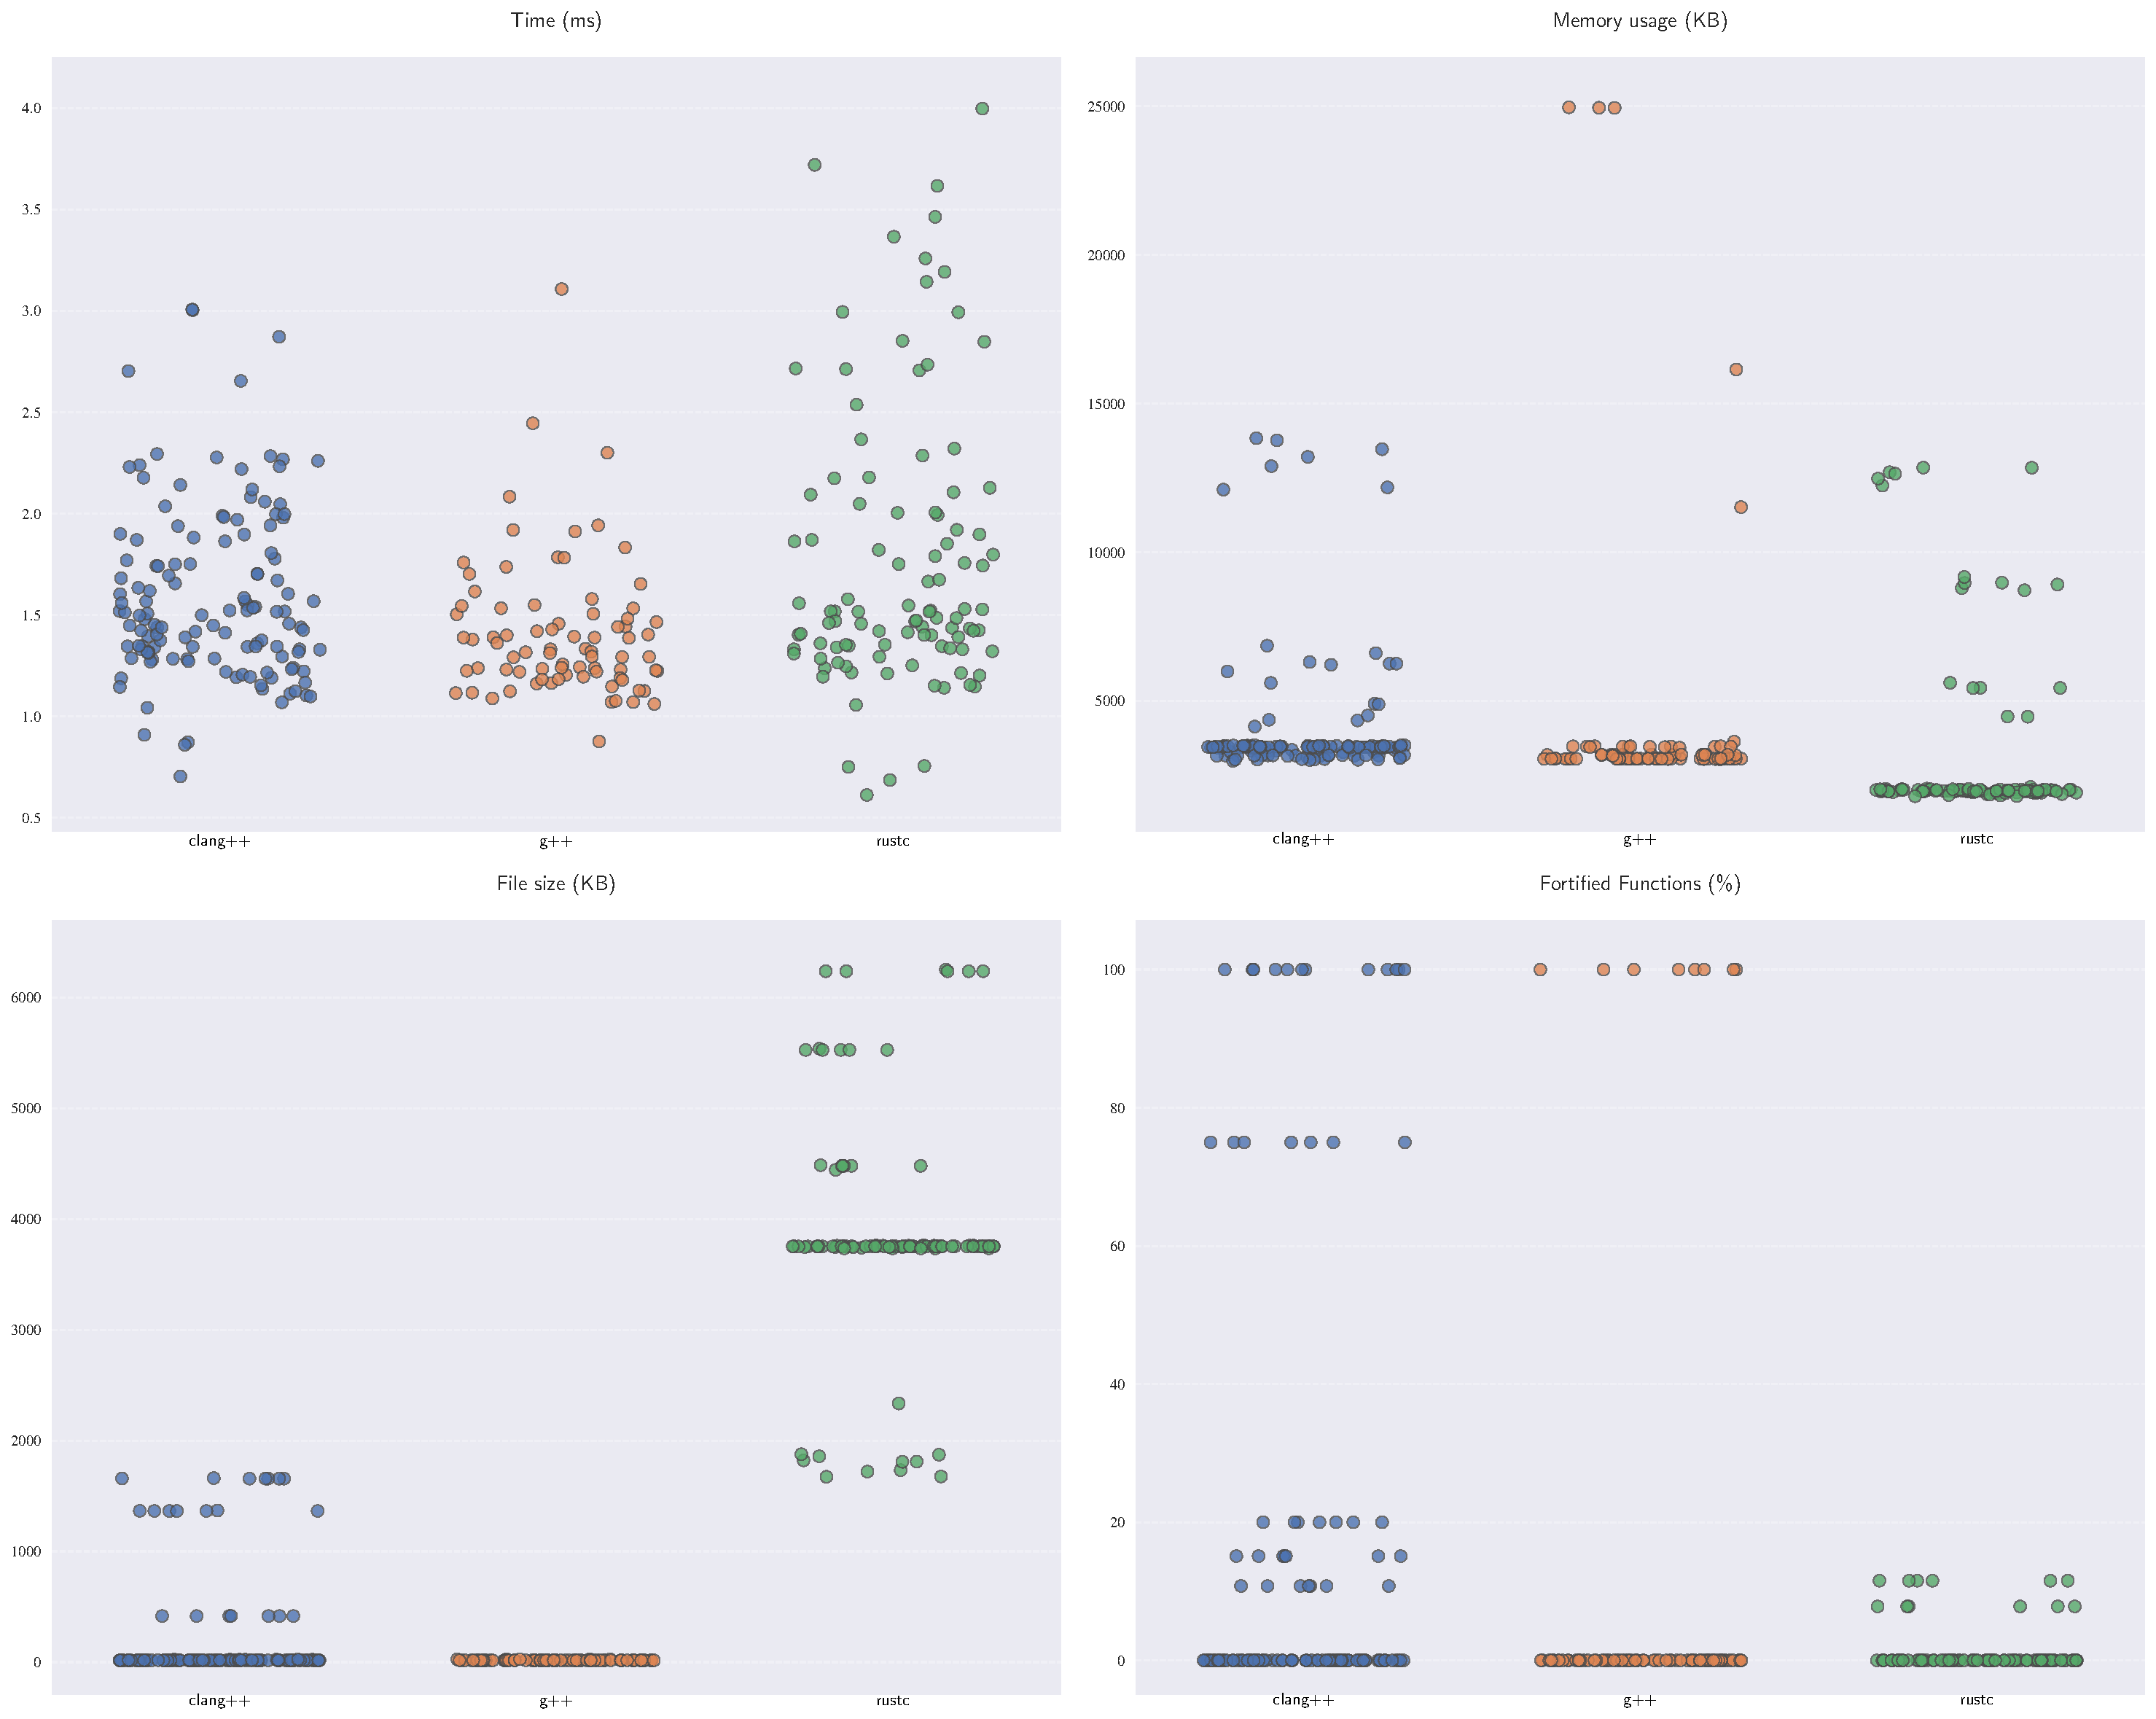
\includegraphics[width=\textwidth, height=0.85\textheight, keepaspectratio]{Gráficas/./Facet_Grid.pdf}
  \caption{Facet Grid}
  \label{fig:Gráficas_facet_grid}
\end{figure}
\newpage

% === Gráficas_cualitativas/Comparacion_compiladores ===
\subsection*{Comparacion Compiladores}
\begin{figure}[htbp]
  \centering
  
\includegraphics[width=\textwidth, height=0.85\textheight, keepaspectratio]{Gráficas/Gráficas_cualitativas/Comparacion_compiladores.pdf}
  \caption{Comparacion Compiladores}
  \label{fig:Gráficas_gráficas_cualitativas_comparacion_compiladores}
\end{figure}
\newpage

% === Gráficas_cualitativas/Gráfico_protecciones ===
\subsection*{Gráfico Protecciones}
\begin{figure}[htbp]
  \centering
  
\includegraphics[width=\textwidth, height=0.85\textheight, keepaspectratio]{Gráficas/Gráficas_cualitativas/Gráfico_protecciones.pdf}
  \caption{Gráfico Protecciones}
  \label{fig:Gráficas_gráficas_cualitativas_gráfico_protecciones}
\end{figure}
\newpage

\section*{Gráficas Por Optimización}

% === Gráficas_por_optimización/-O0 ===
\subsection*{-O0}
\begin{figure}[htbp]
  \centering
  \caption{Resultados de compilación con optimización \texttt{-O0}}
  \vspace{0.5cm}

  \begin{minipage}{0.48\textwidth}
    \centering
    \subfloat[Tamaño del archivo (KB)]{
      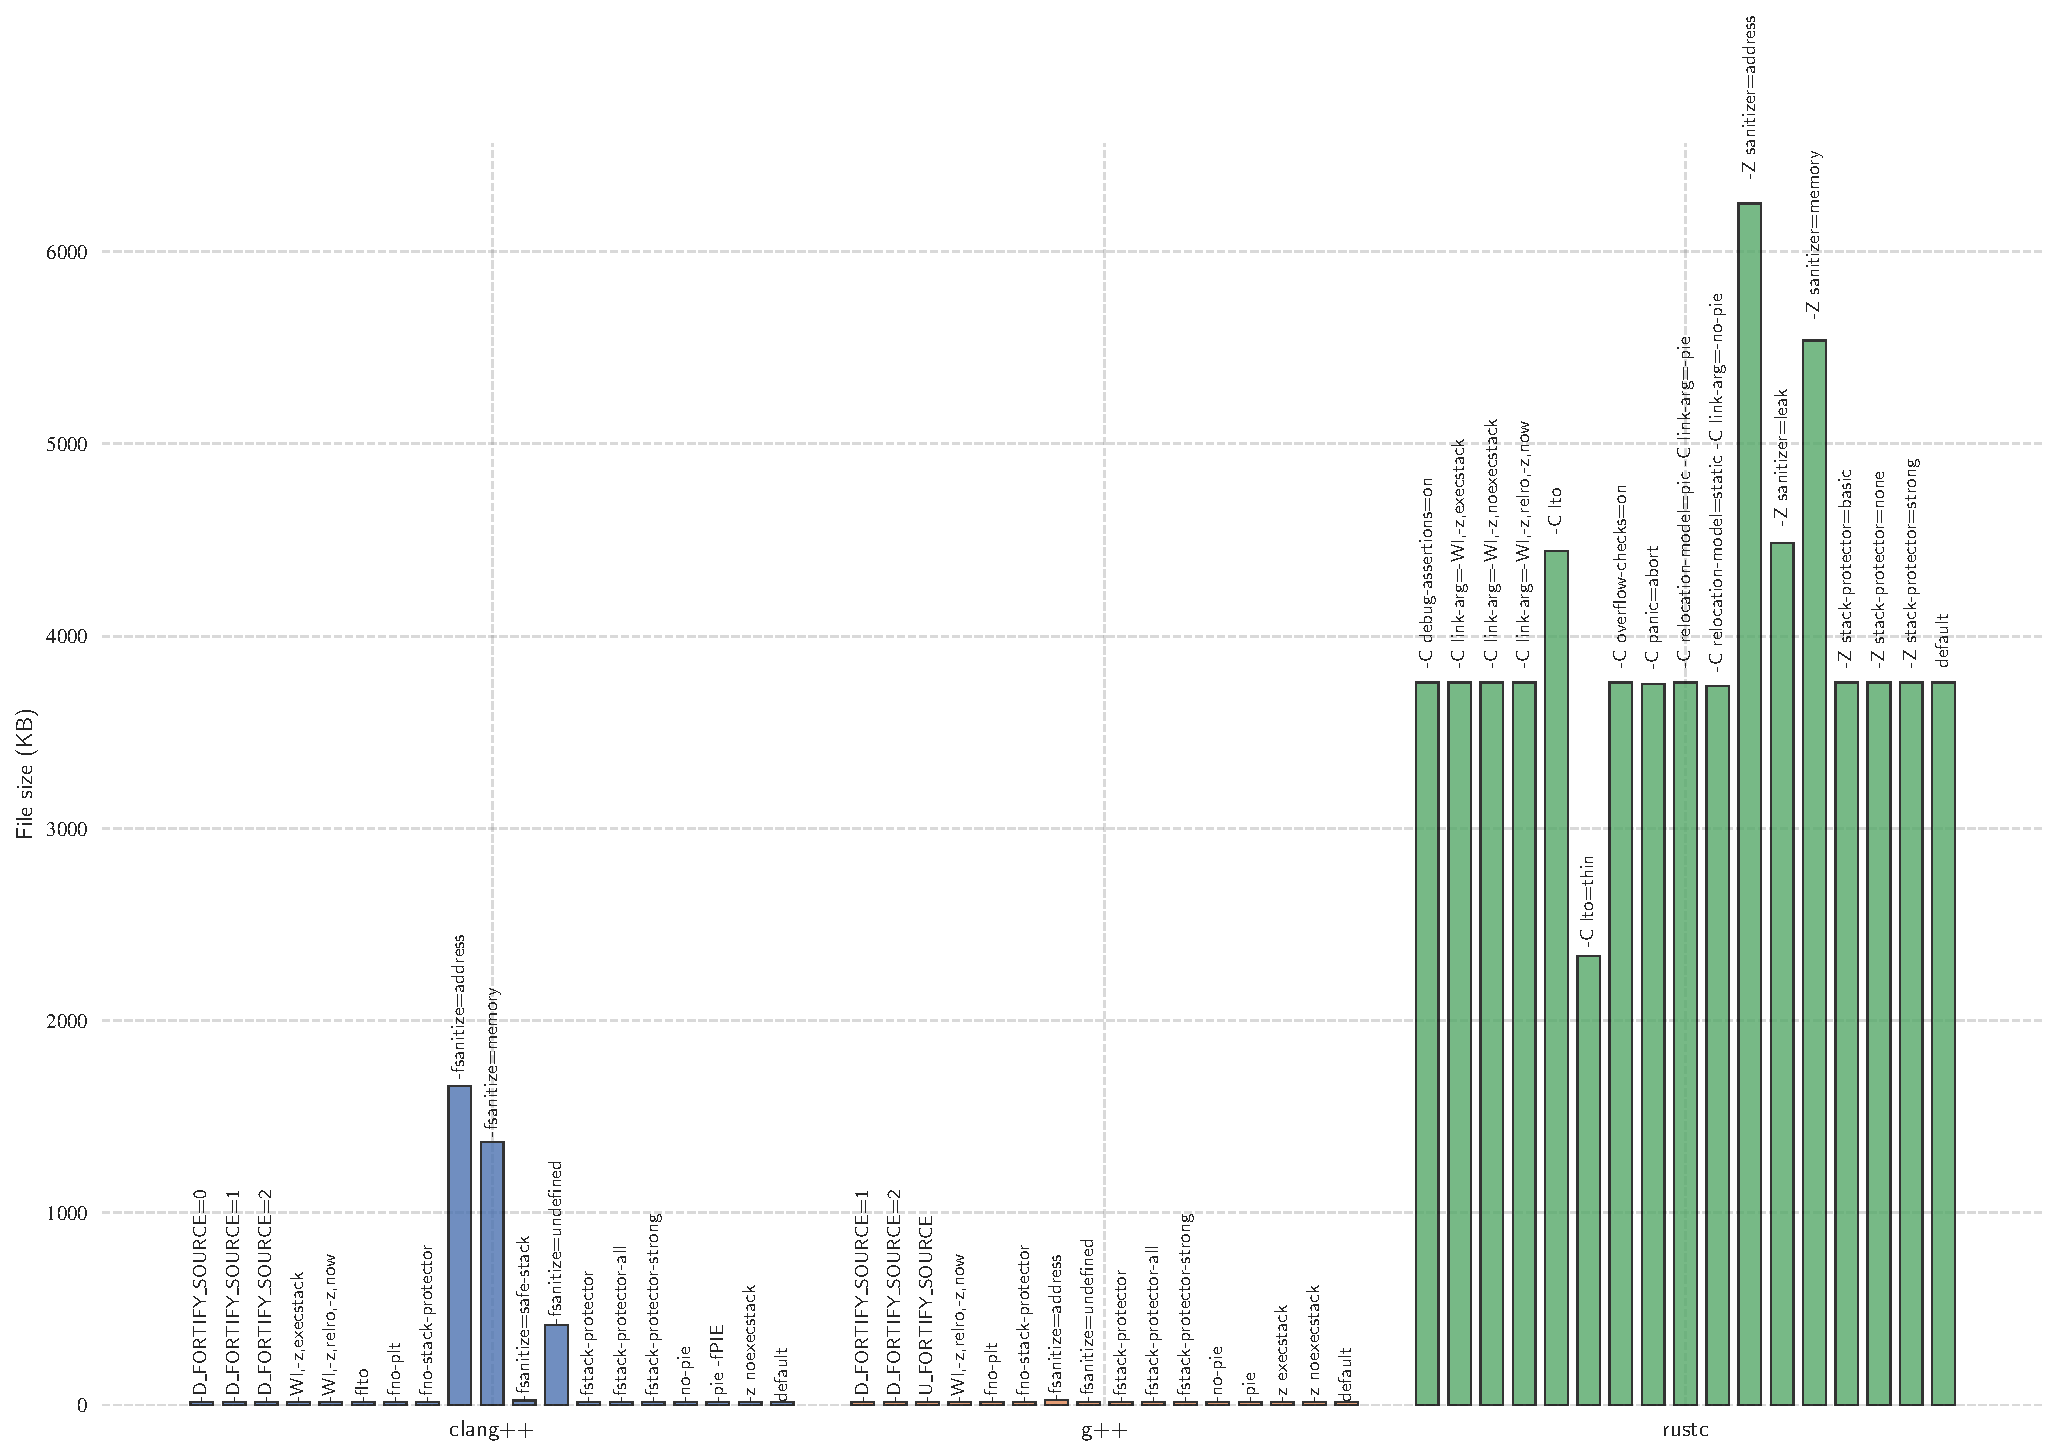
\includegraphics[width=\linewidth]{Gráficas/Gráficas_por_optimización/-O0/File_size_KB.pdf}
      \label{fig:Gráficas_gráficas_por_optimización__o0_file_size_kb}
    }
  \end{minipage}
  \hfill
  \begin{minipage}{0.48\textwidth}
    \centering
    \subfloat[Funciones fortificadas (\%)]{
      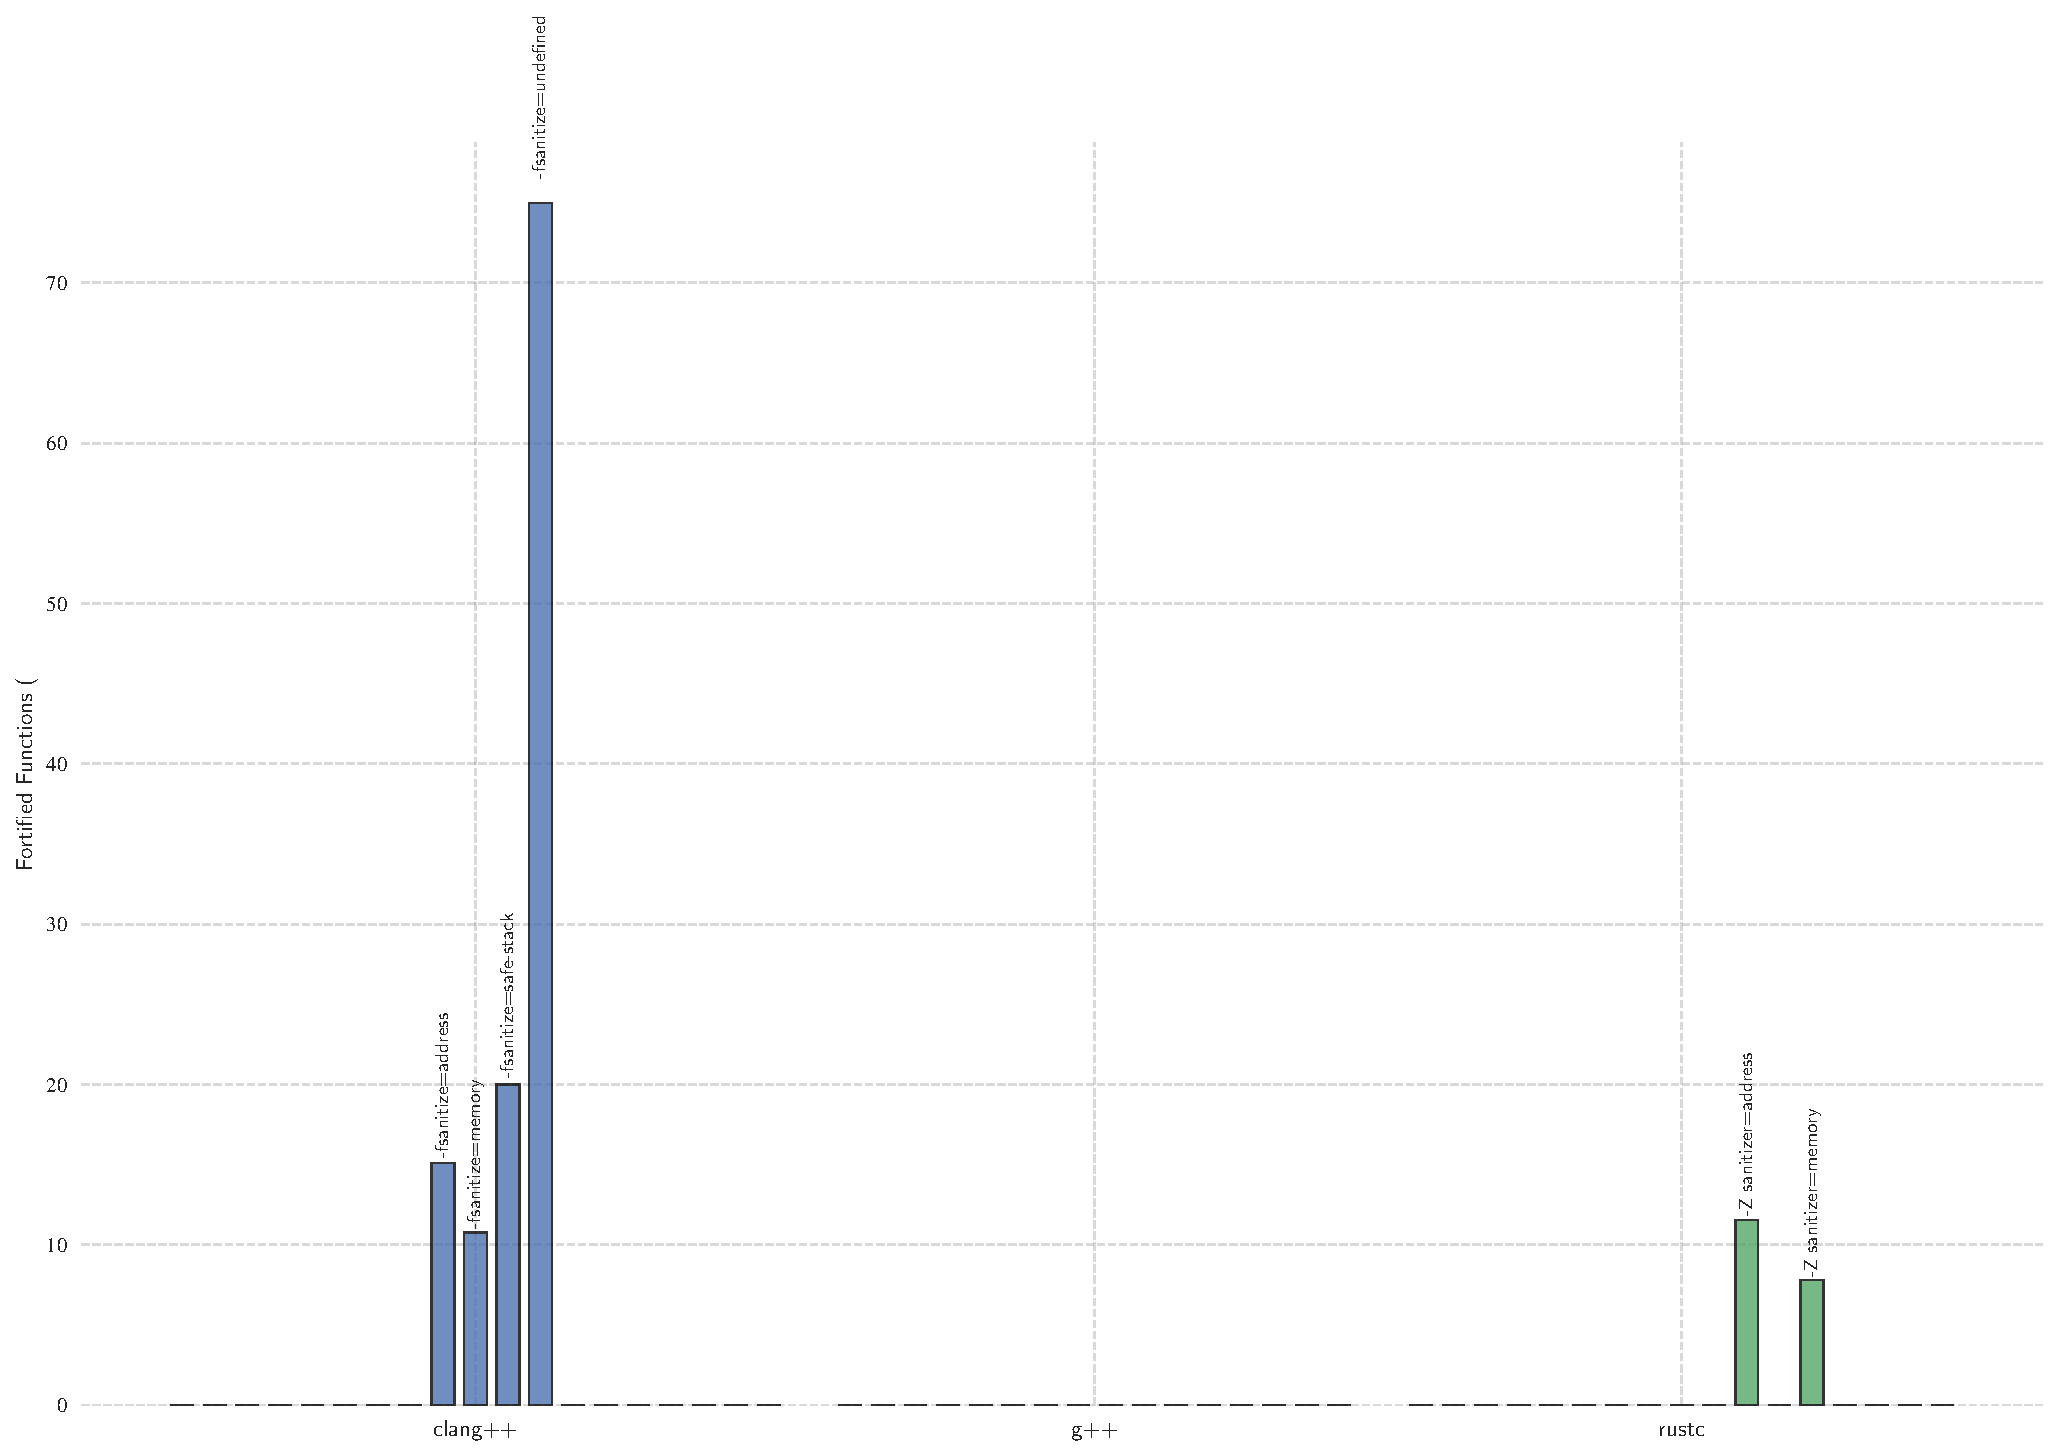
\includegraphics[width=\linewidth]{Gráficas/Gráficas_por_optimización/-O0/Fortified_Functions.pdf}
      \label{fig:Gráficas_gráficas_por_optimización__o0_fortified_functions}
    }
  \end{minipage}


  \vspace{1cm}

  \begin{minipage}{0.48\textwidth}
    \centering
    \subfloat[Uso de memoria (KB)]{
      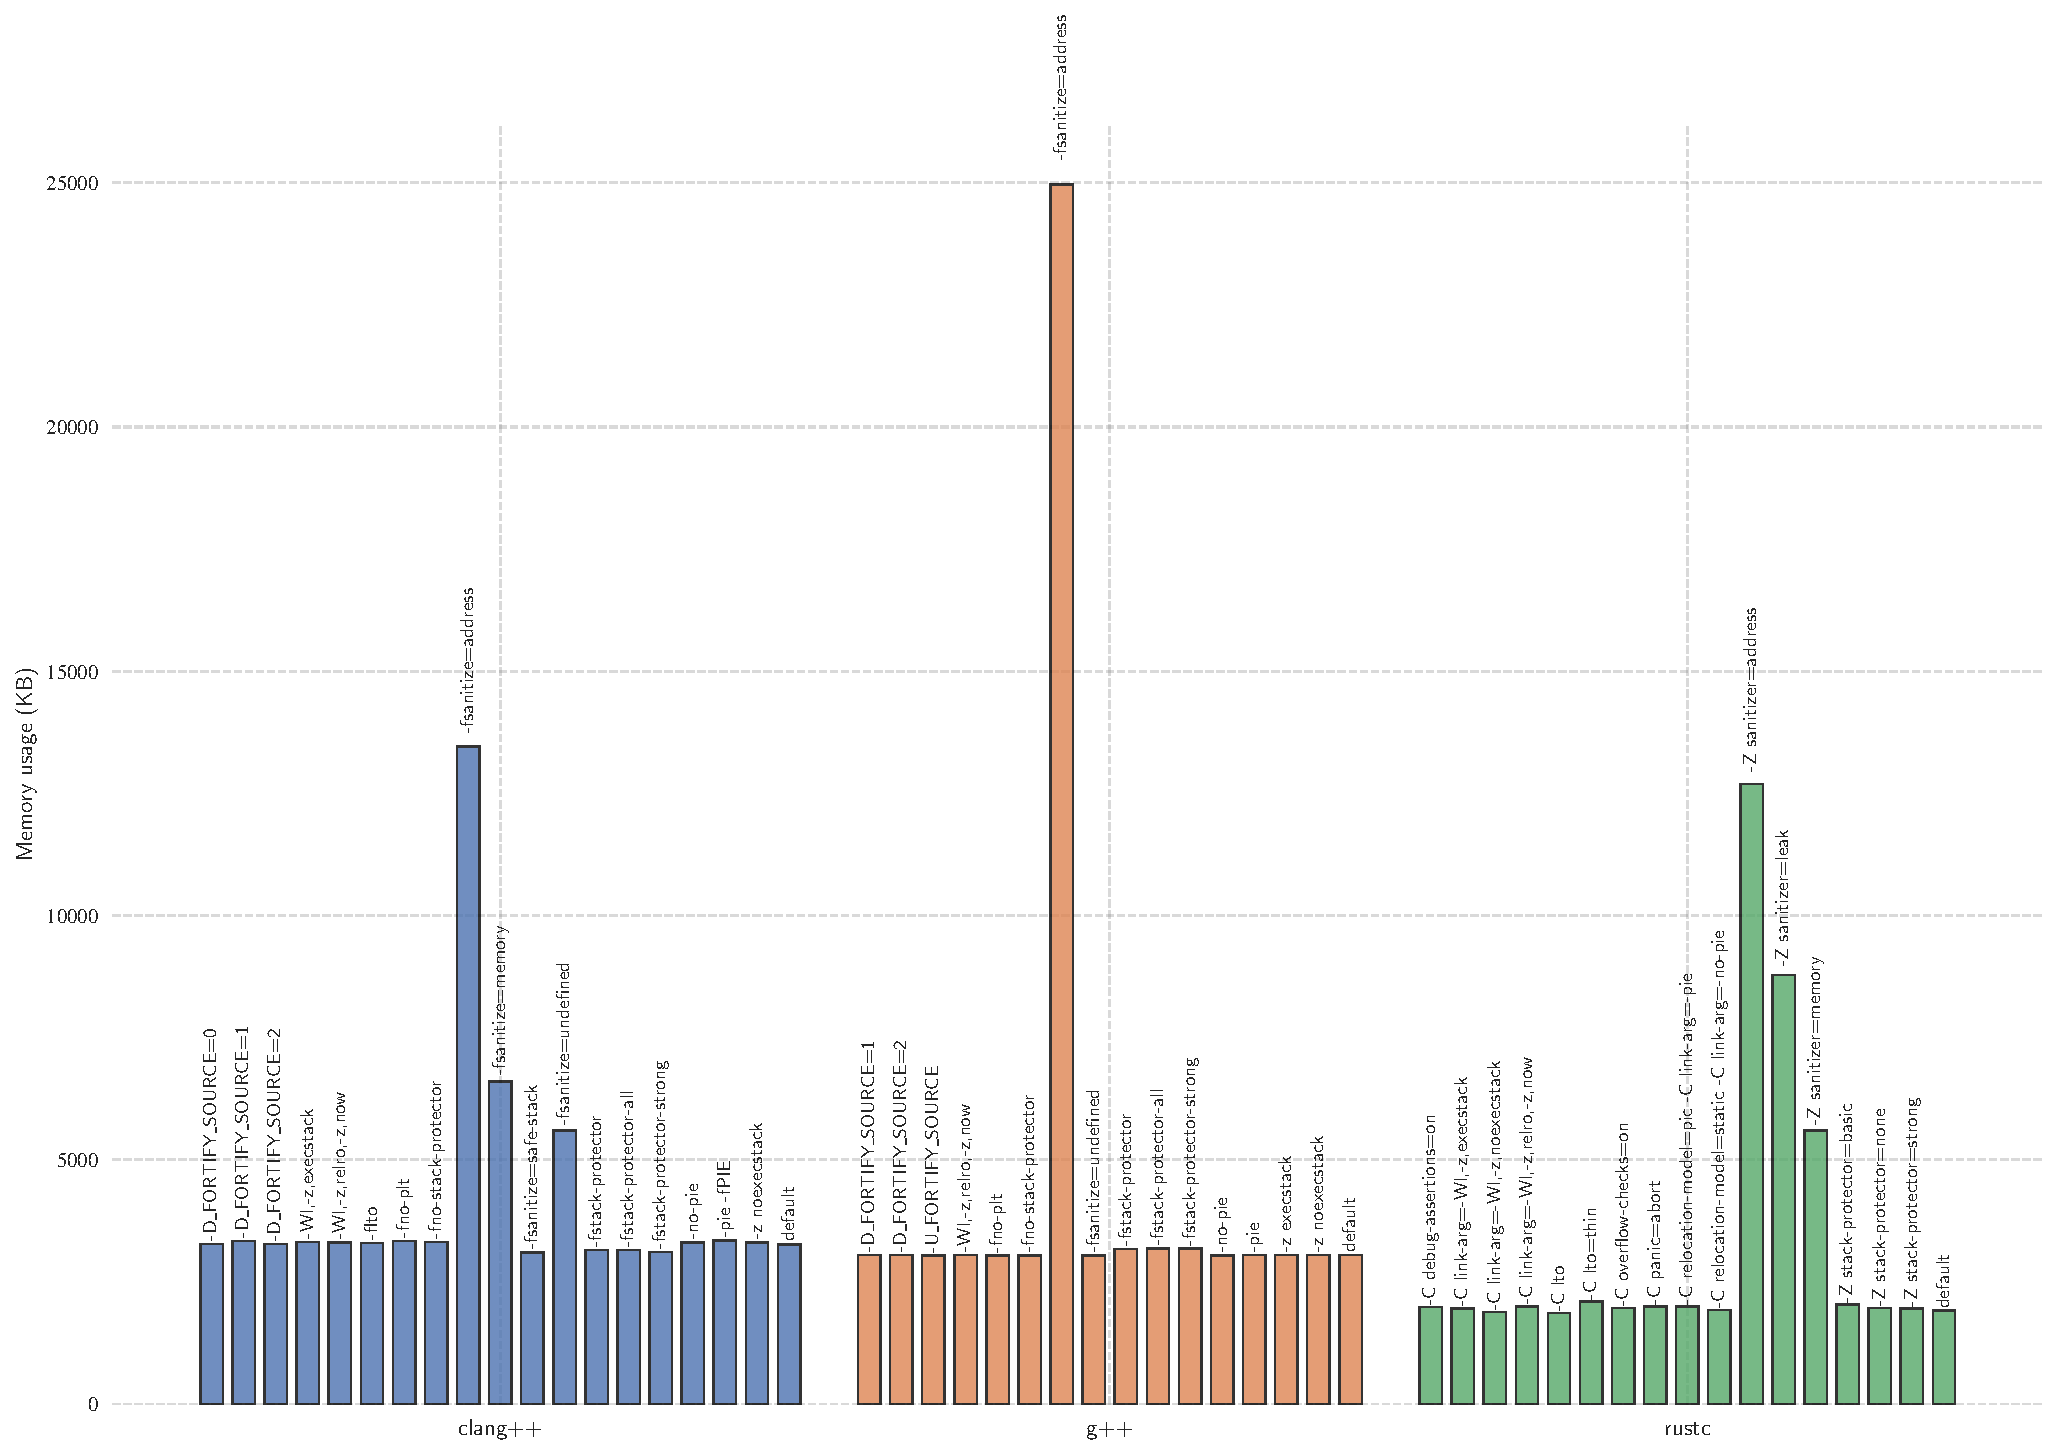
\includegraphics[width=\linewidth]{Gráficas/Gráficas_por_optimización/-O0/Memory_usage_KB.pdf}
      \label{fig:Gráficas_gráficas_por_optimización__o0_memory_usage_kb}
    }
  \end{minipage}
  \hfill
  \begin{minipage}{0.48\textwidth}
    \centering
    \subfloat[Tiempo (ms)]{
      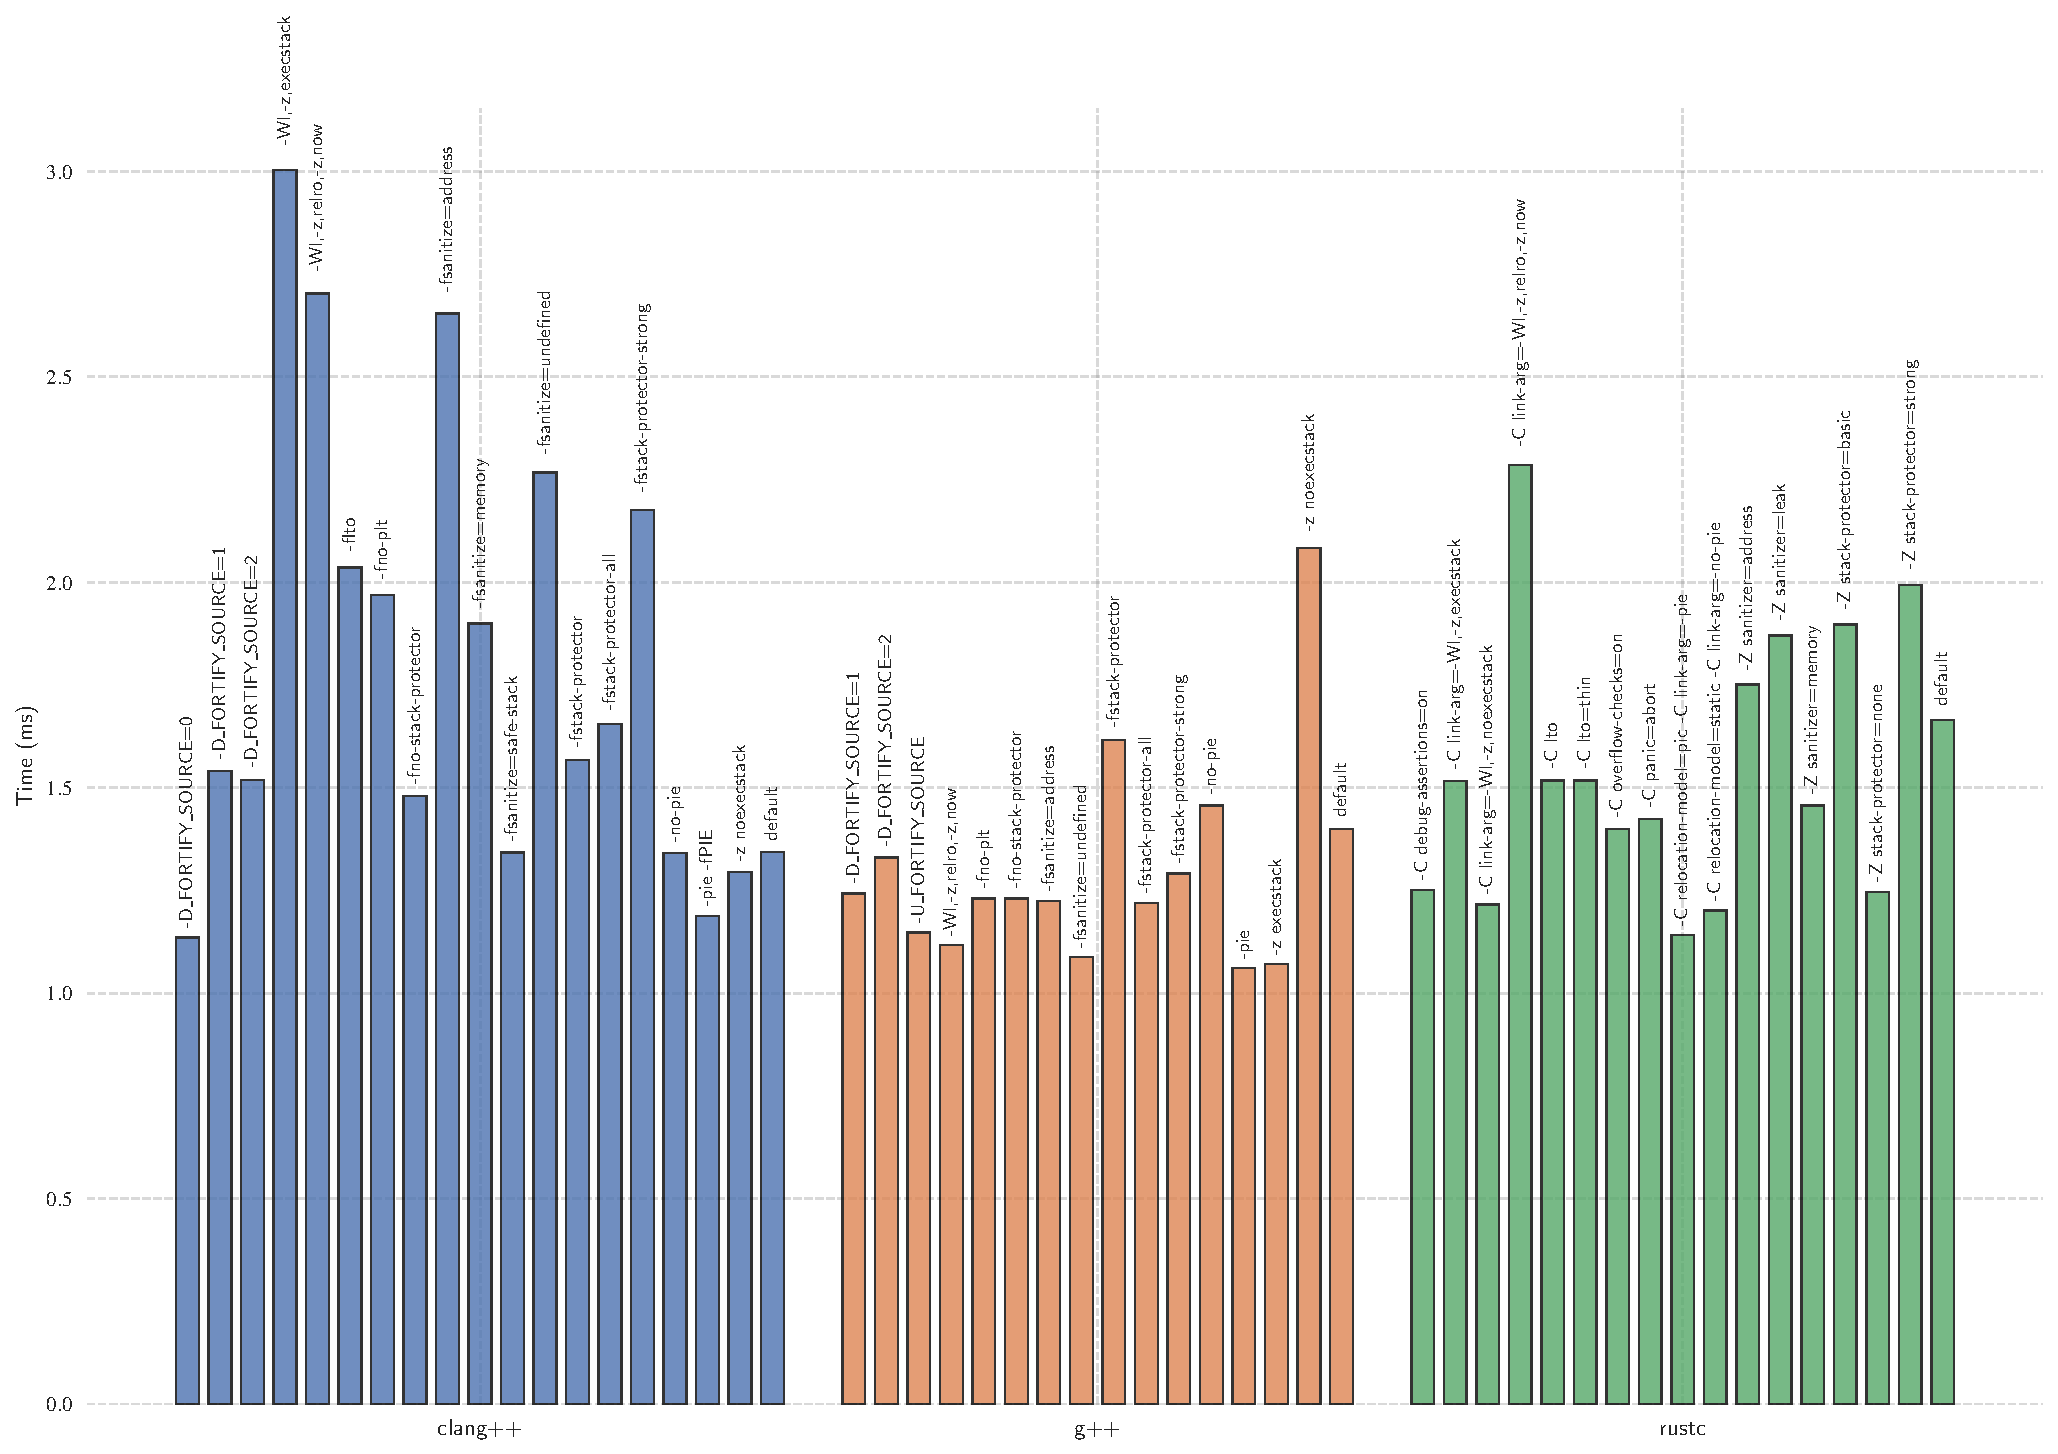
\includegraphics[width=\linewidth]{Gráficas/Gráficas_por_optimización/-O0/Time_ms.pdf}
      \label{fig:Gráficas_gráficas_por_optimización__o0_time_ms}
    }
  \end{minipage}

\end{figure}
\newpage

% === Gráficas_por_optimización/-O1 ===
\subsection*{-O1}
\begin{figure}[htbp]
  \centering
  \caption{Resultados de compilación con optimización \texttt{-O1}}
  \vspace{0.5cm}

  \begin{minipage}{0.48\textwidth}
    \centering
    \subfloat[Tamaño del archivo (KB)]{
      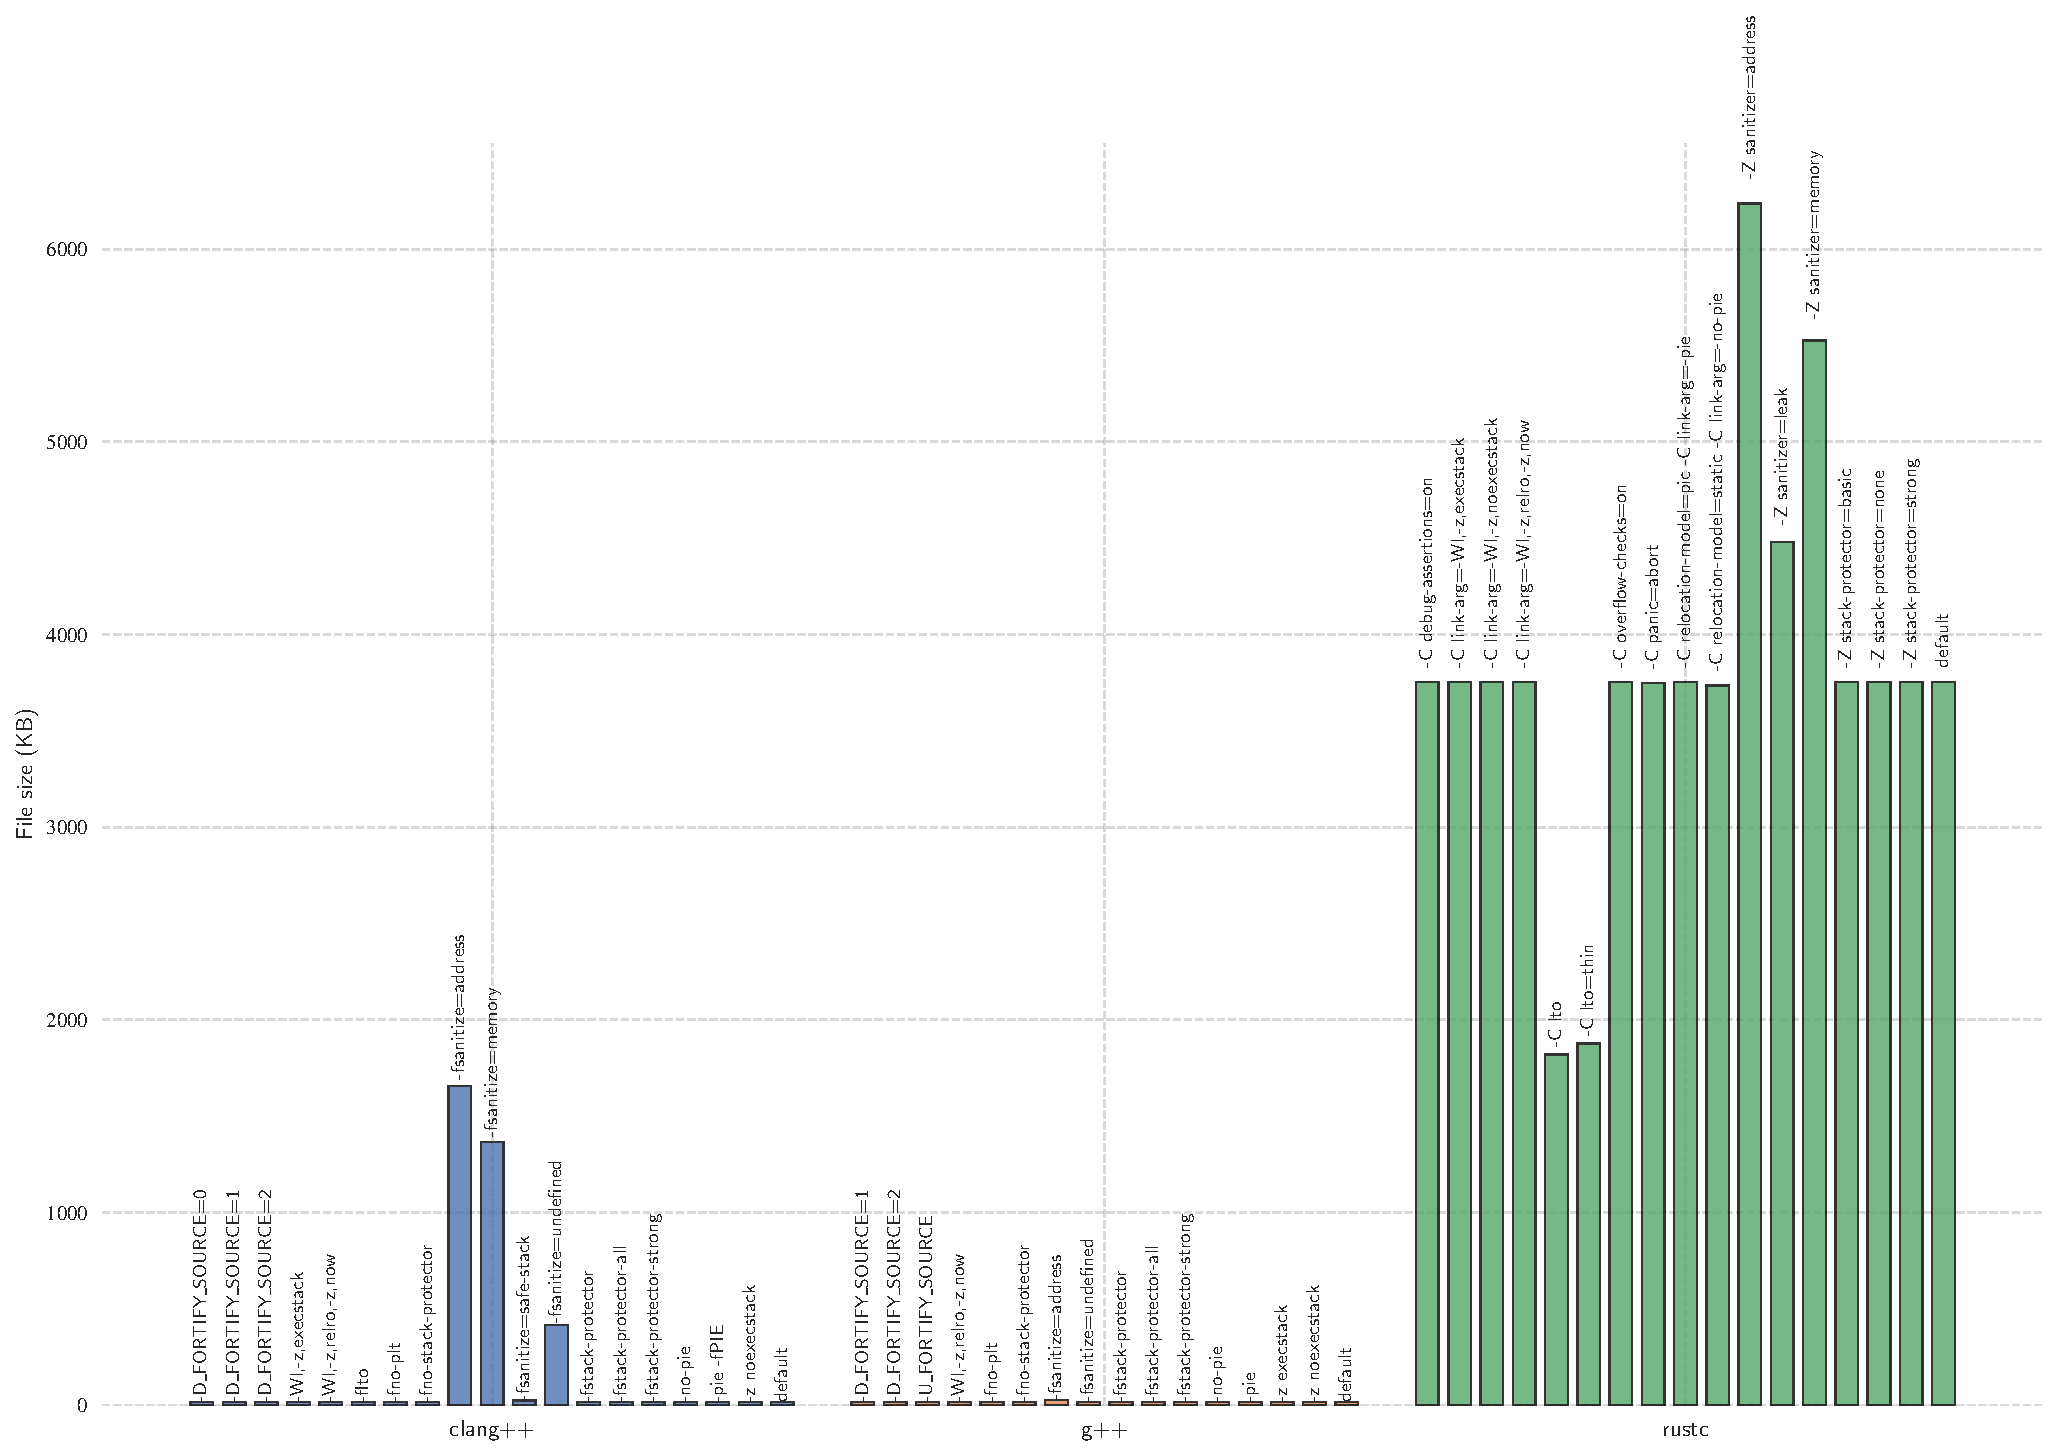
\includegraphics[width=\linewidth]{Gráficas/Gráficas_por_optimización/-O1/File_size_KB.pdf}
      \label{fig:Gráficas_gráficas_por_optimización__o1_file_size_kb}
    }
  \end{minipage}
  \hfill
  \begin{minipage}{0.48\textwidth}
    \centering
    \subfloat[Funciones fortificadas (\%)]{
      \includegraphics[width=\linewidth]{Gráficas/Gráficas_por_optimización/-O1/Fortified_Functions.pdf}
      \label{fig:Gráficas_gráficas_por_optimización__o1_fortified_functions}
    }
  \end{minipage}


  \vspace{1cm}

  \begin{minipage}{0.48\textwidth}
    \centering
    \subfloat[Uso de memoria (KB)]{
      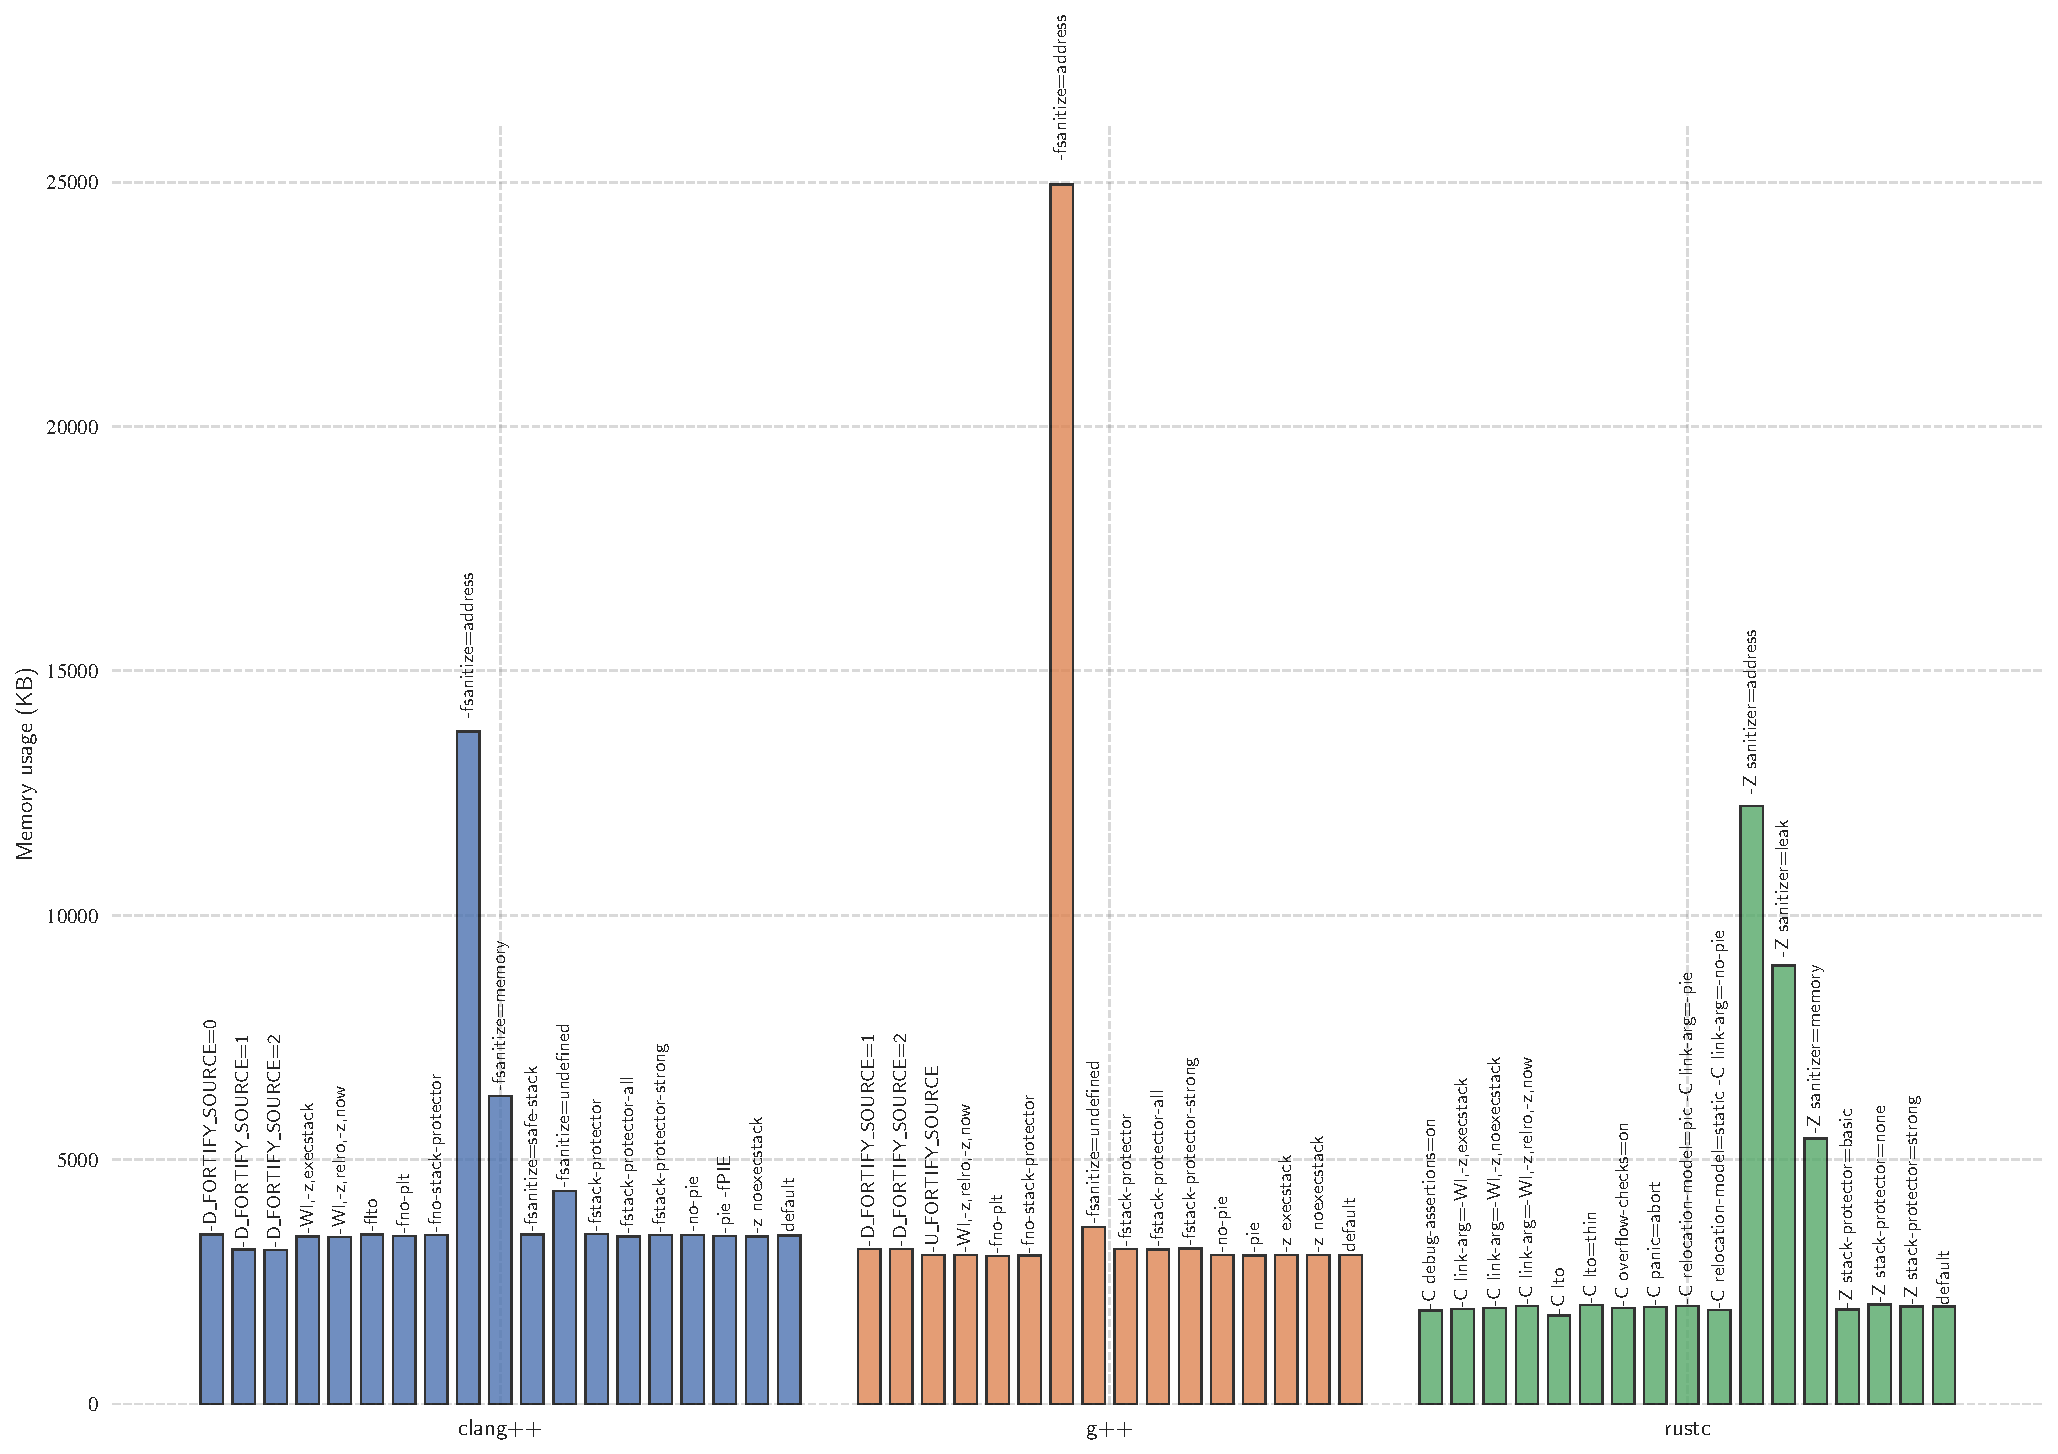
\includegraphics[width=\linewidth]{Gráficas/Gráficas_por_optimización/-O1/Memory_usage_KB.pdf}
      \label{fig:Gráficas_gráficas_por_optimización__o1_memory_usage_kb}
    }
  \end{minipage}
  \hfill
  \begin{minipage}{0.48\textwidth}
    \centering
    \subfloat[Tiempo (ms)]{
      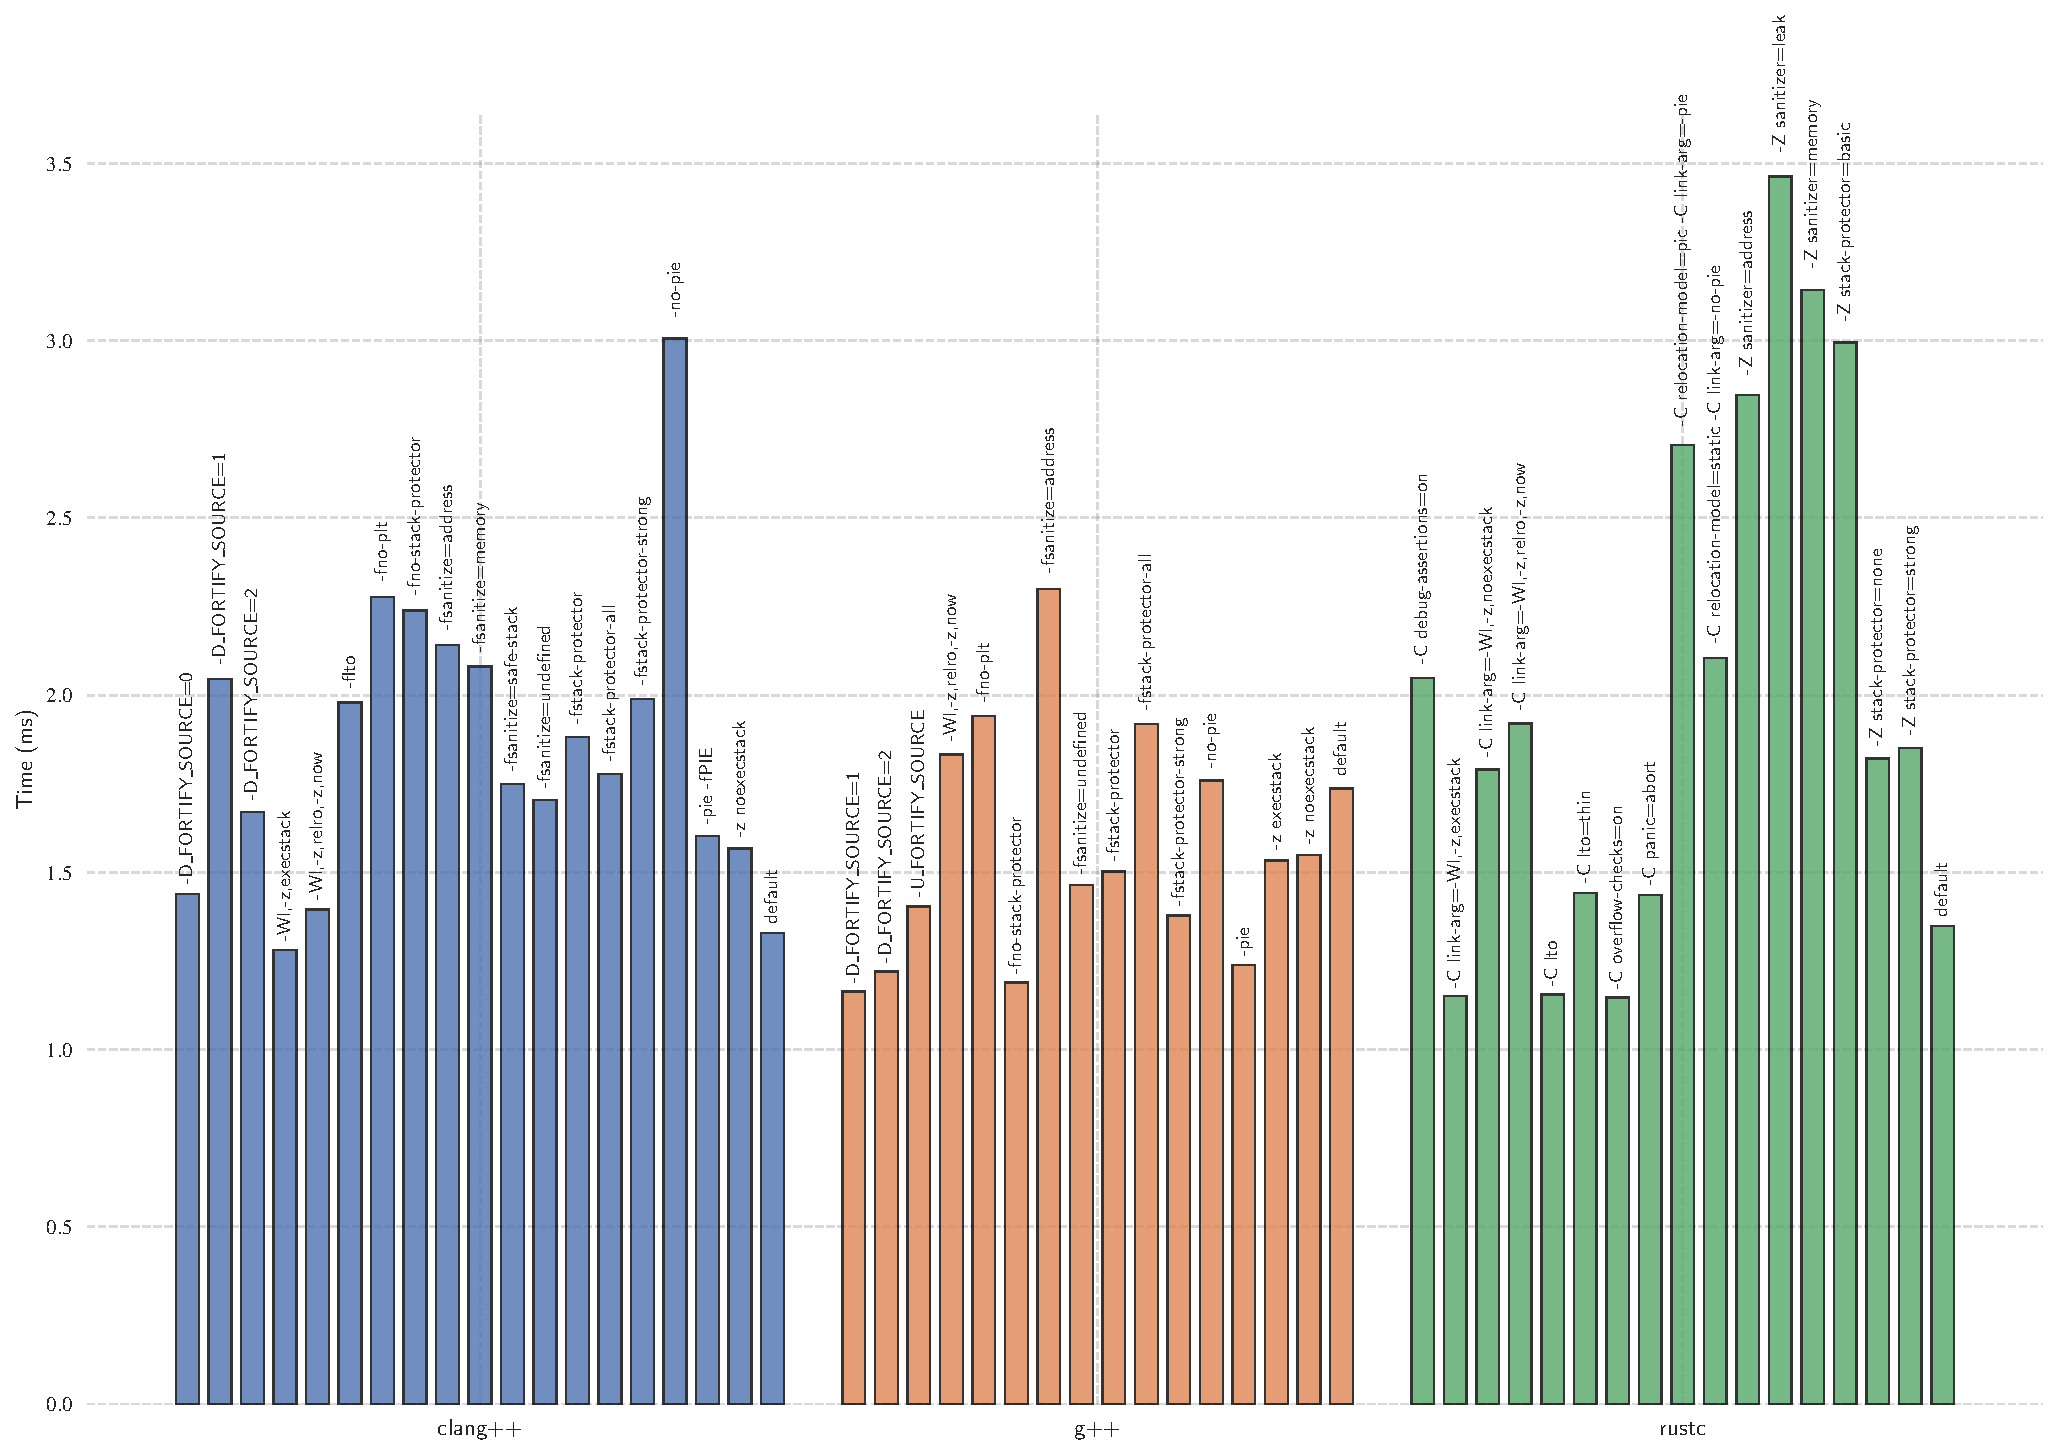
\includegraphics[width=\linewidth]{Gráficas/Gráficas_por_optimización/-O1/Time_ms.pdf}
      \label{fig:Gráficas_gráficas_por_optimización__o1_time_ms}
    }
  \end{minipage}

\end{figure}
\newpage

% === Gráficas_por_optimización/-O2 ===
\subsection*{-O2}
\begin{figure}[htbp]
  \centering
  \caption{Resultados de compilación con optimización \texttt{-O2}}
  \vspace{0.5cm}

  \begin{minipage}{0.48\textwidth}
    \centering
    \subfloat[Tamaño del archivo (KB)]{
      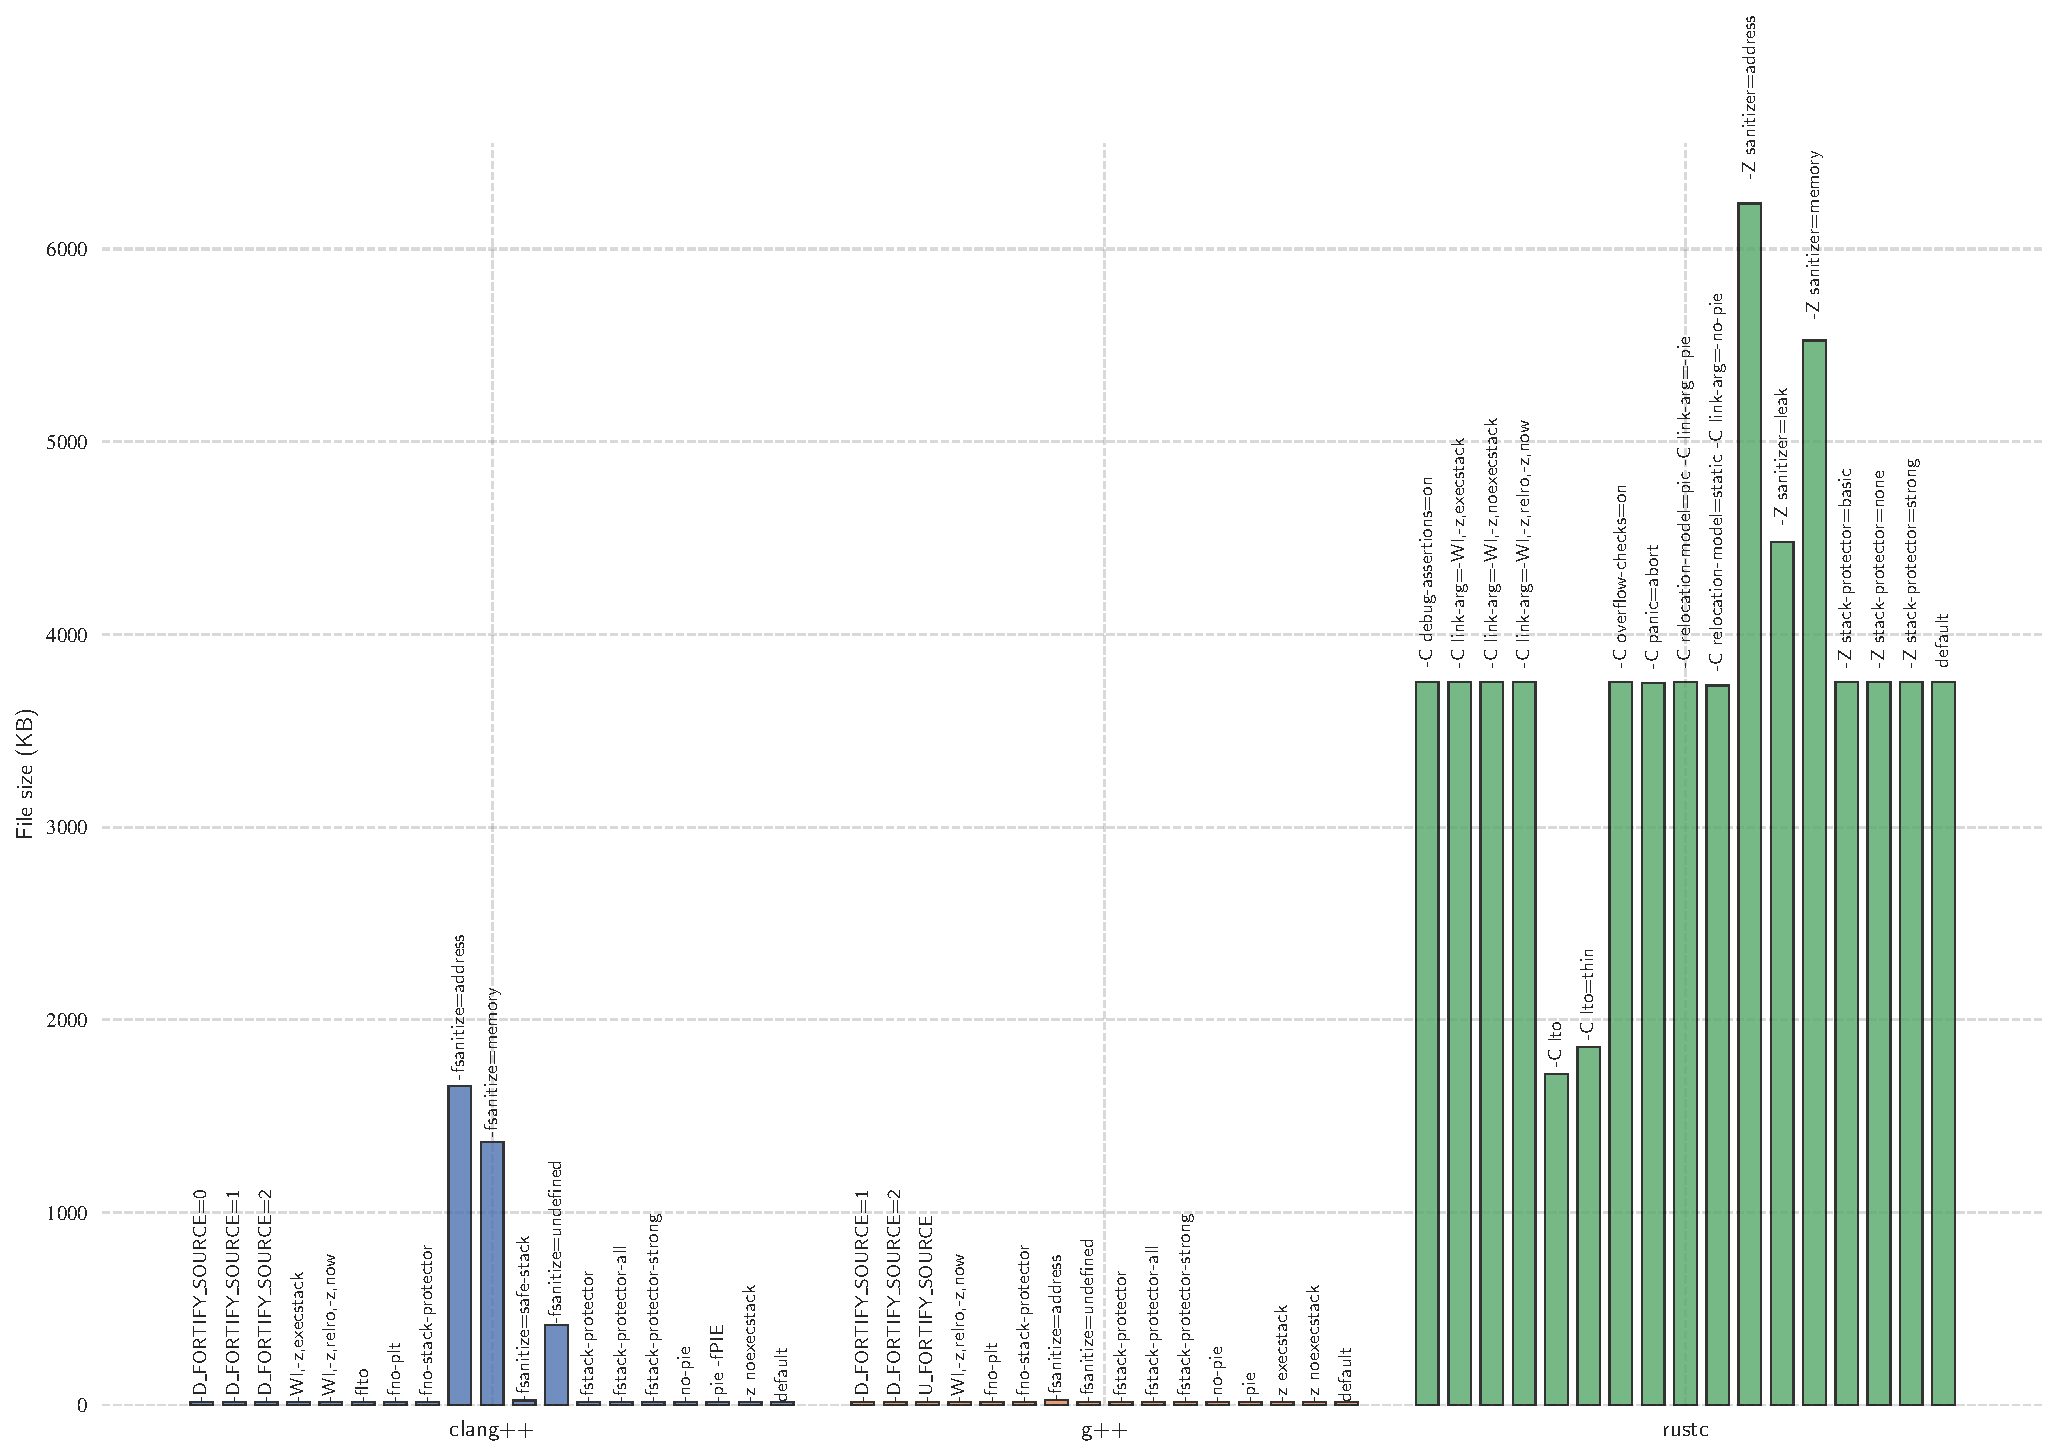
\includegraphics[width=\linewidth]{Gráficas/Gráficas_por_optimización/-O2/File_size_KB.pdf}
      \label{fig:Gráficas_gráficas_por_optimización__o2_file_size_kb}
    }
  \end{minipage}
  \hfill
  \begin{minipage}{0.48\textwidth}
    \centering
    \subfloat[Funciones fortificadas (\%)]{
      \includegraphics[width=\linewidth]{Gráficas/Gráficas_por_optimización/-O2/Fortified_Functions.pdf}
      \label{fig:Gráficas_gráficas_por_optimización__o2_fortified_functions}
    }
  \end{minipage}


  \vspace{1cm}

  \begin{minipage}{0.48\textwidth}
    \centering
    \subfloat[Uso de memoria (KB)]{
      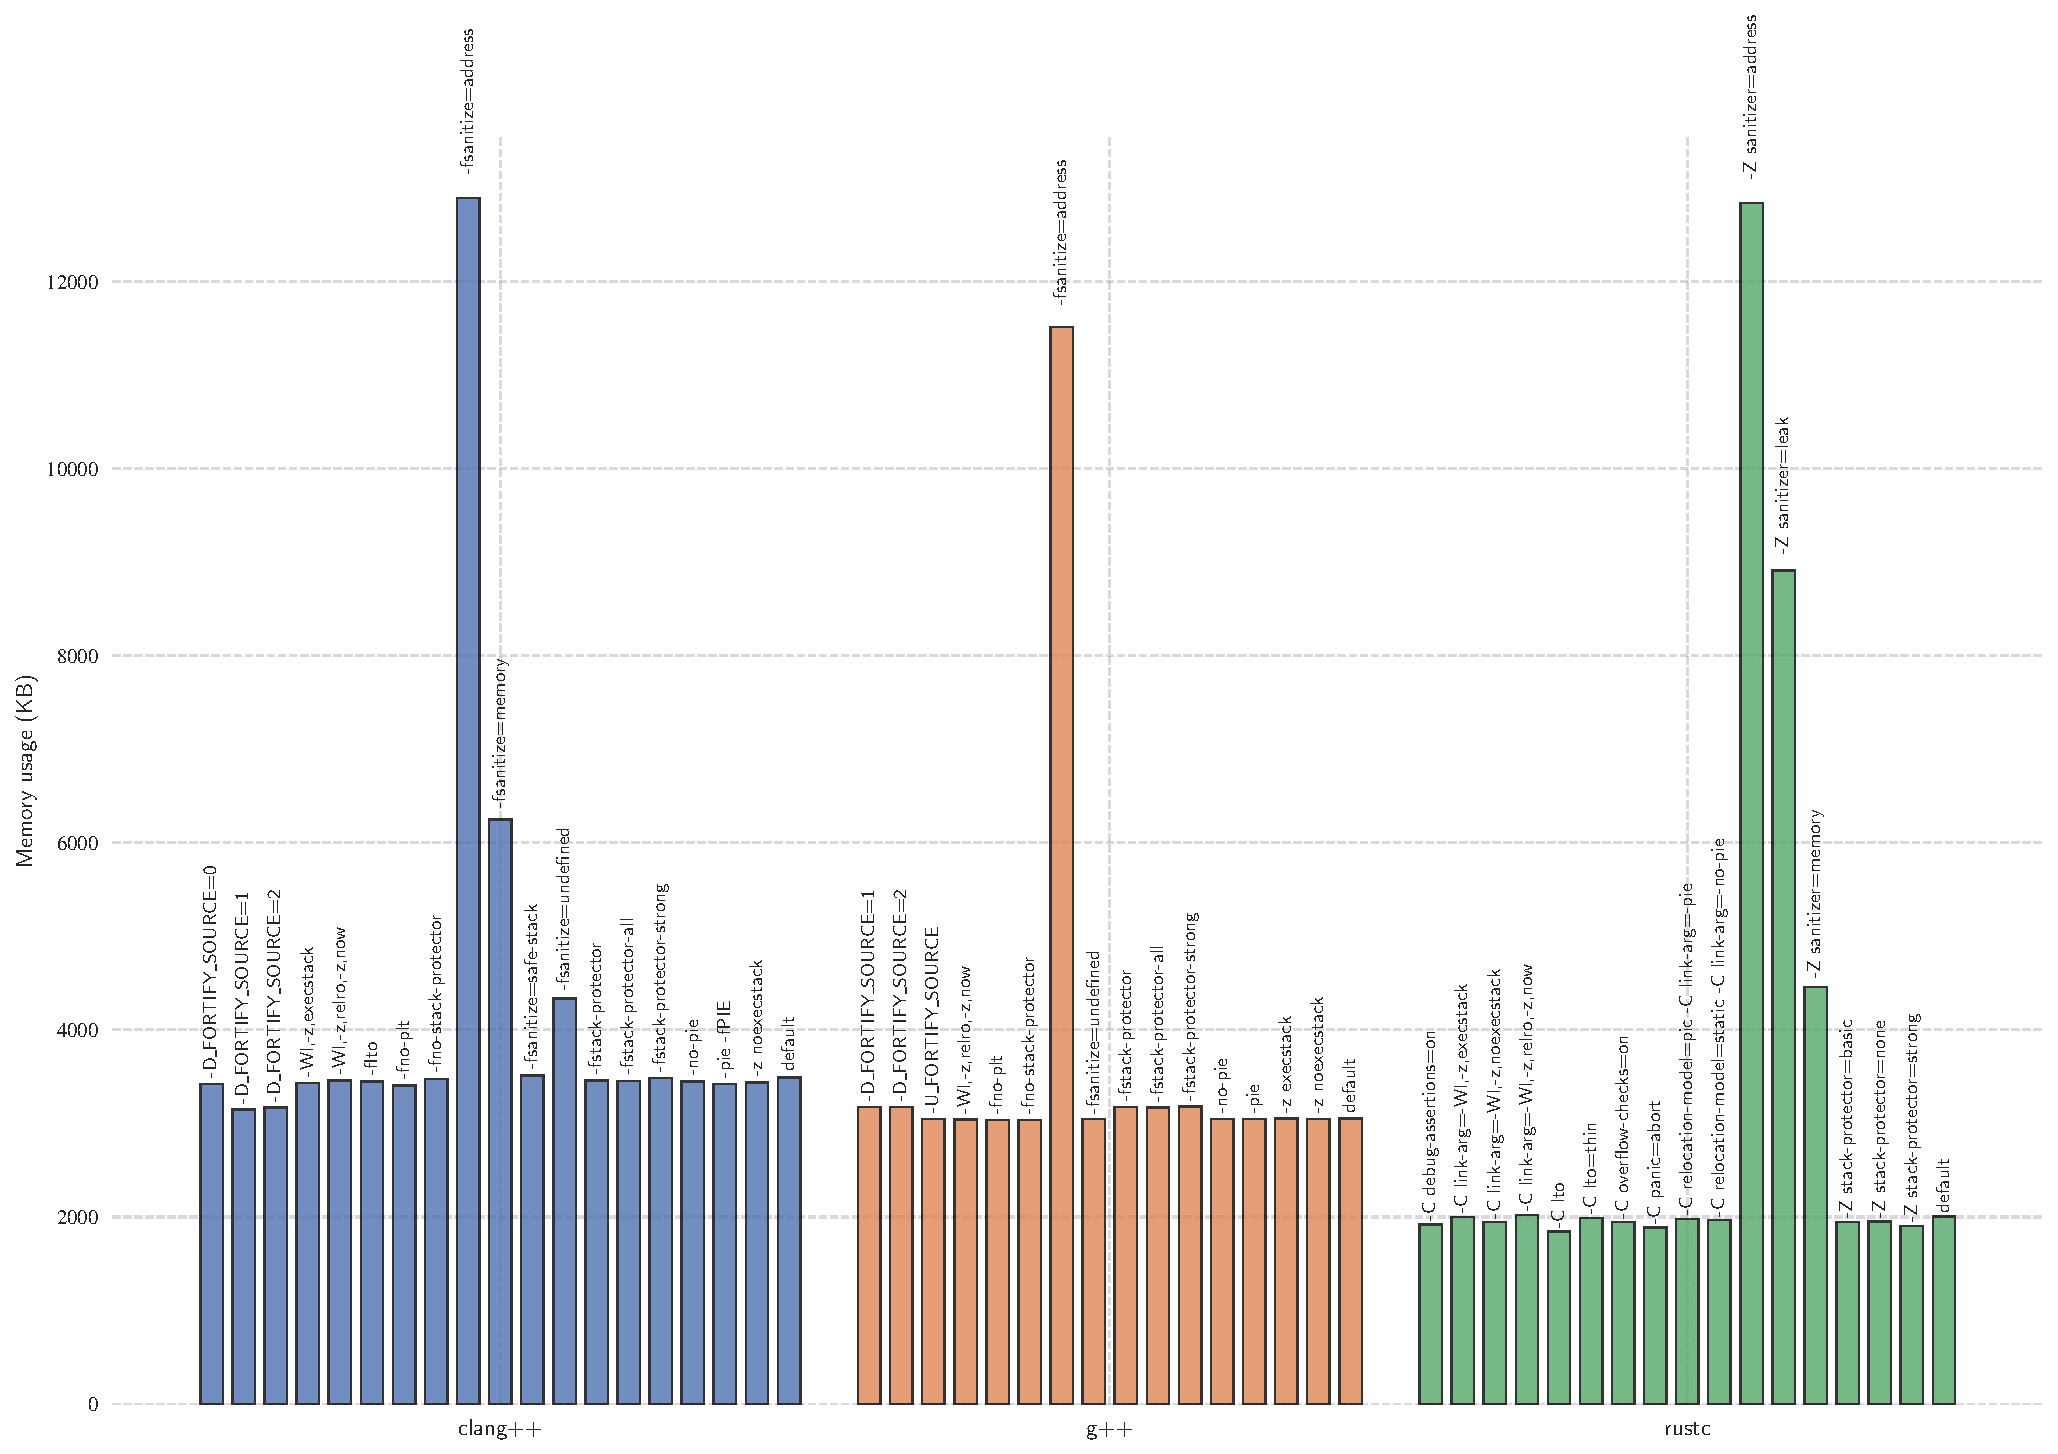
\includegraphics[width=\linewidth]{Gráficas/Gráficas_por_optimización/-O2/Memory_usage_KB.pdf}
      \label{fig:Gráficas_gráficas_por_optimización__o2_memory_usage_kb}
    }
  \end{minipage}
  \hfill
  \begin{minipage}{0.48\textwidth}
    \centering
    \subfloat[Tiempo (ms)]{
      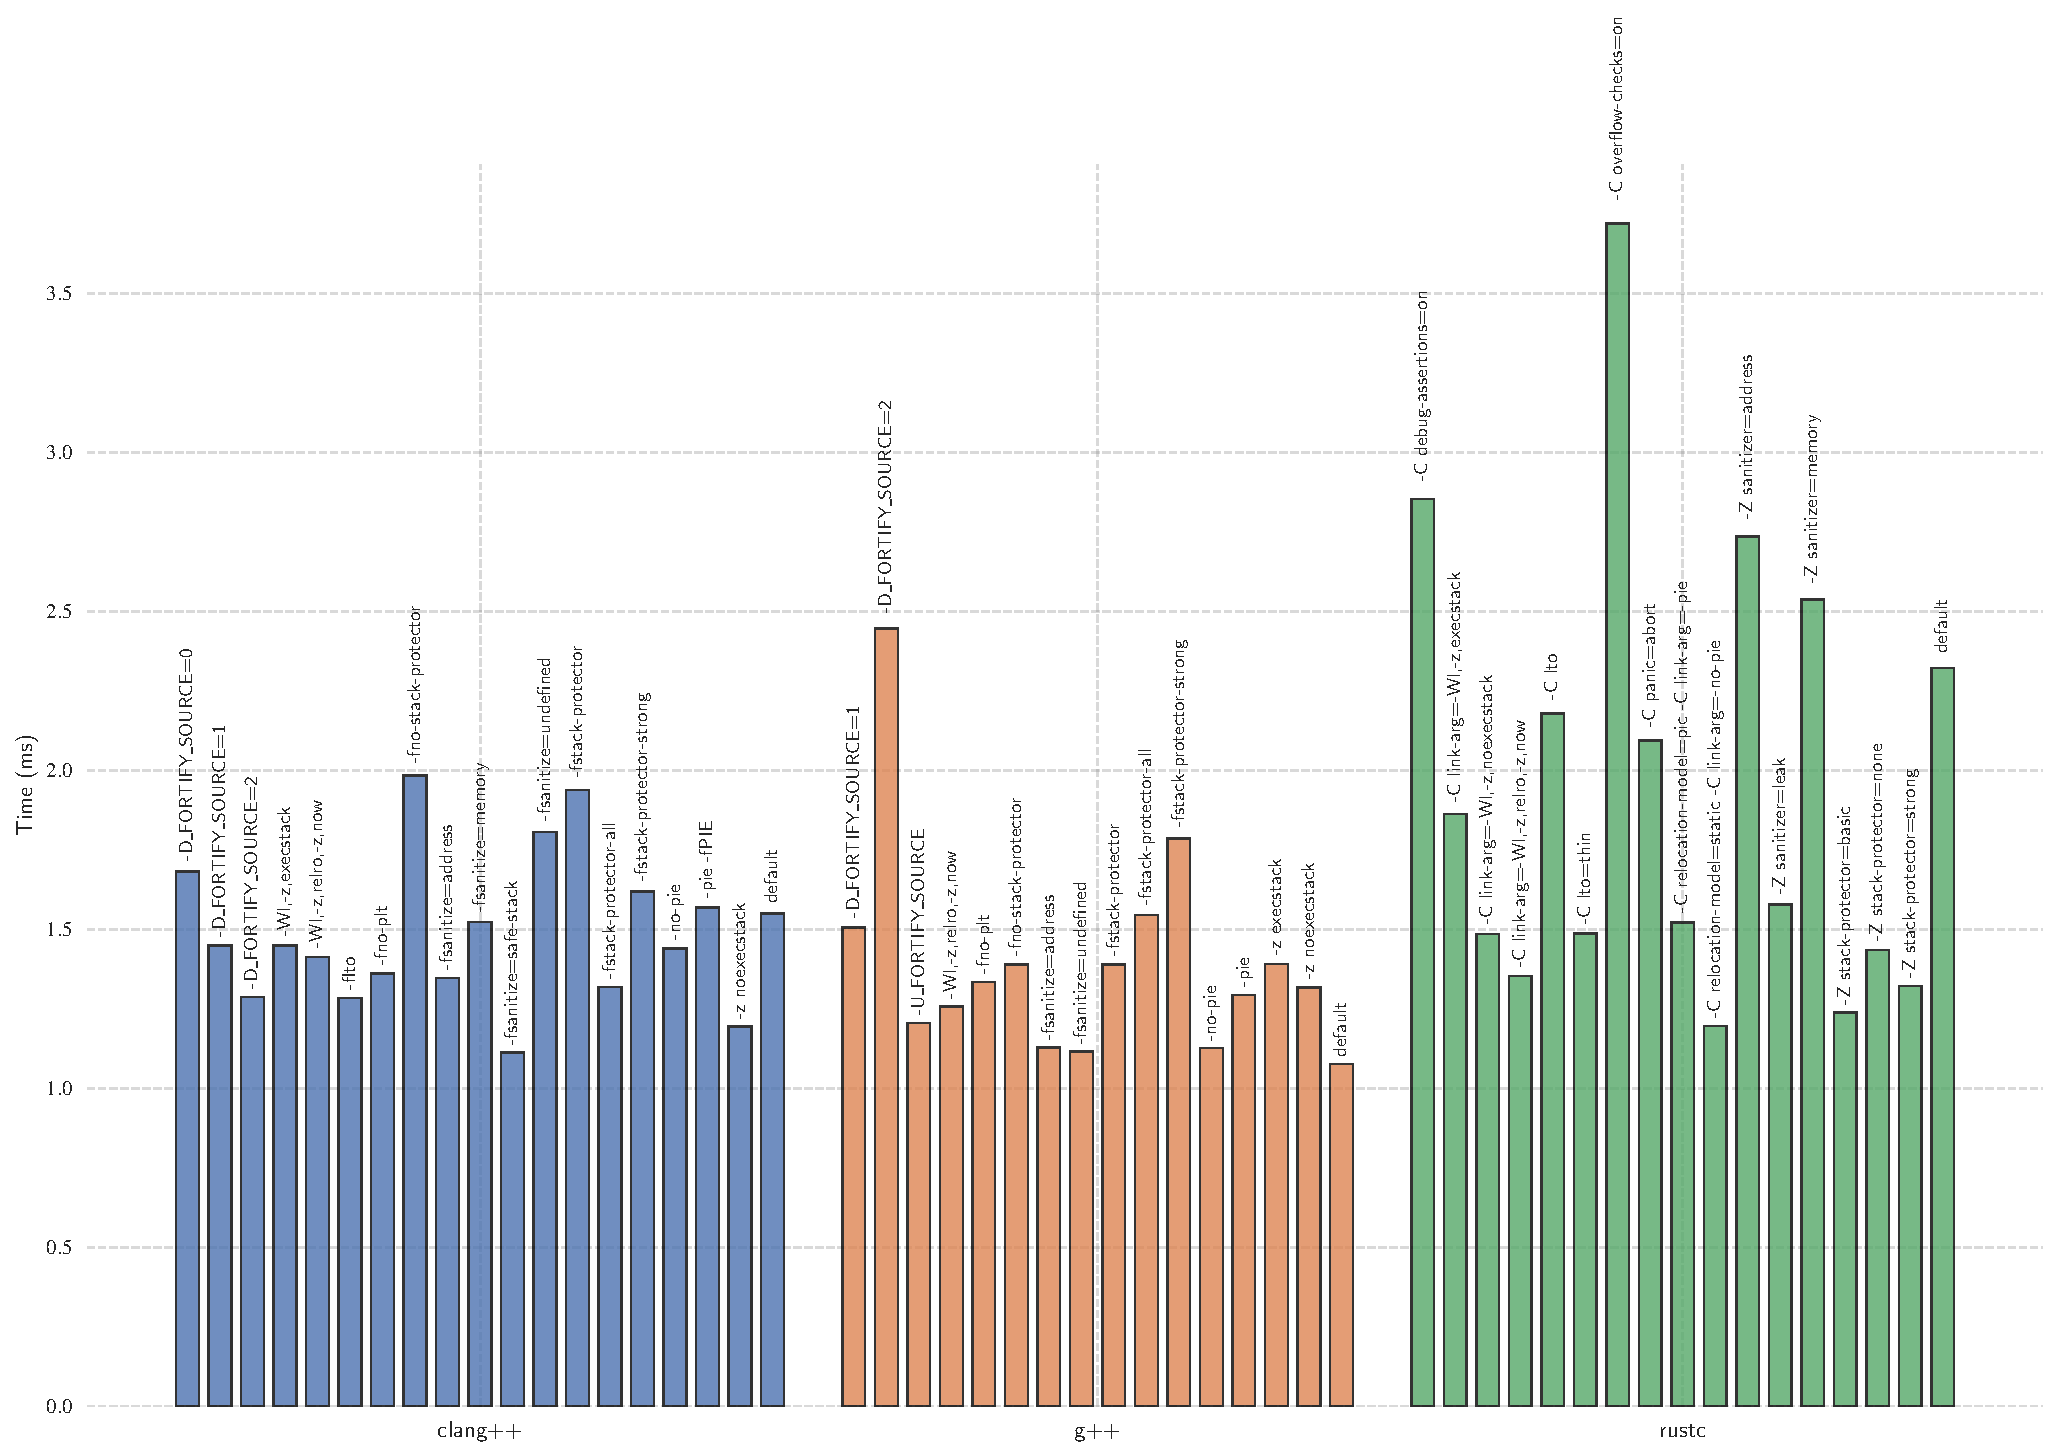
\includegraphics[width=\linewidth]{Gráficas/Gráficas_por_optimización/-O2/Time_ms.pdf}
      \label{fig:Gráficas_gráficas_por_optimización__o2_time_ms}
    }
  \end{minipage}

\end{figure}
\newpage

% === Gráficas_por_optimización/-O3 ===
\subsection*{-O3}
\begin{figure}[htbp]
  \centering
  \caption{Resultados de compilación con optimización \texttt{-O3}}
  \vspace{0.5cm}

  \begin{minipage}{0.48\textwidth}
    \centering
    \subfloat[Tamaño del archivo (KB)]{
      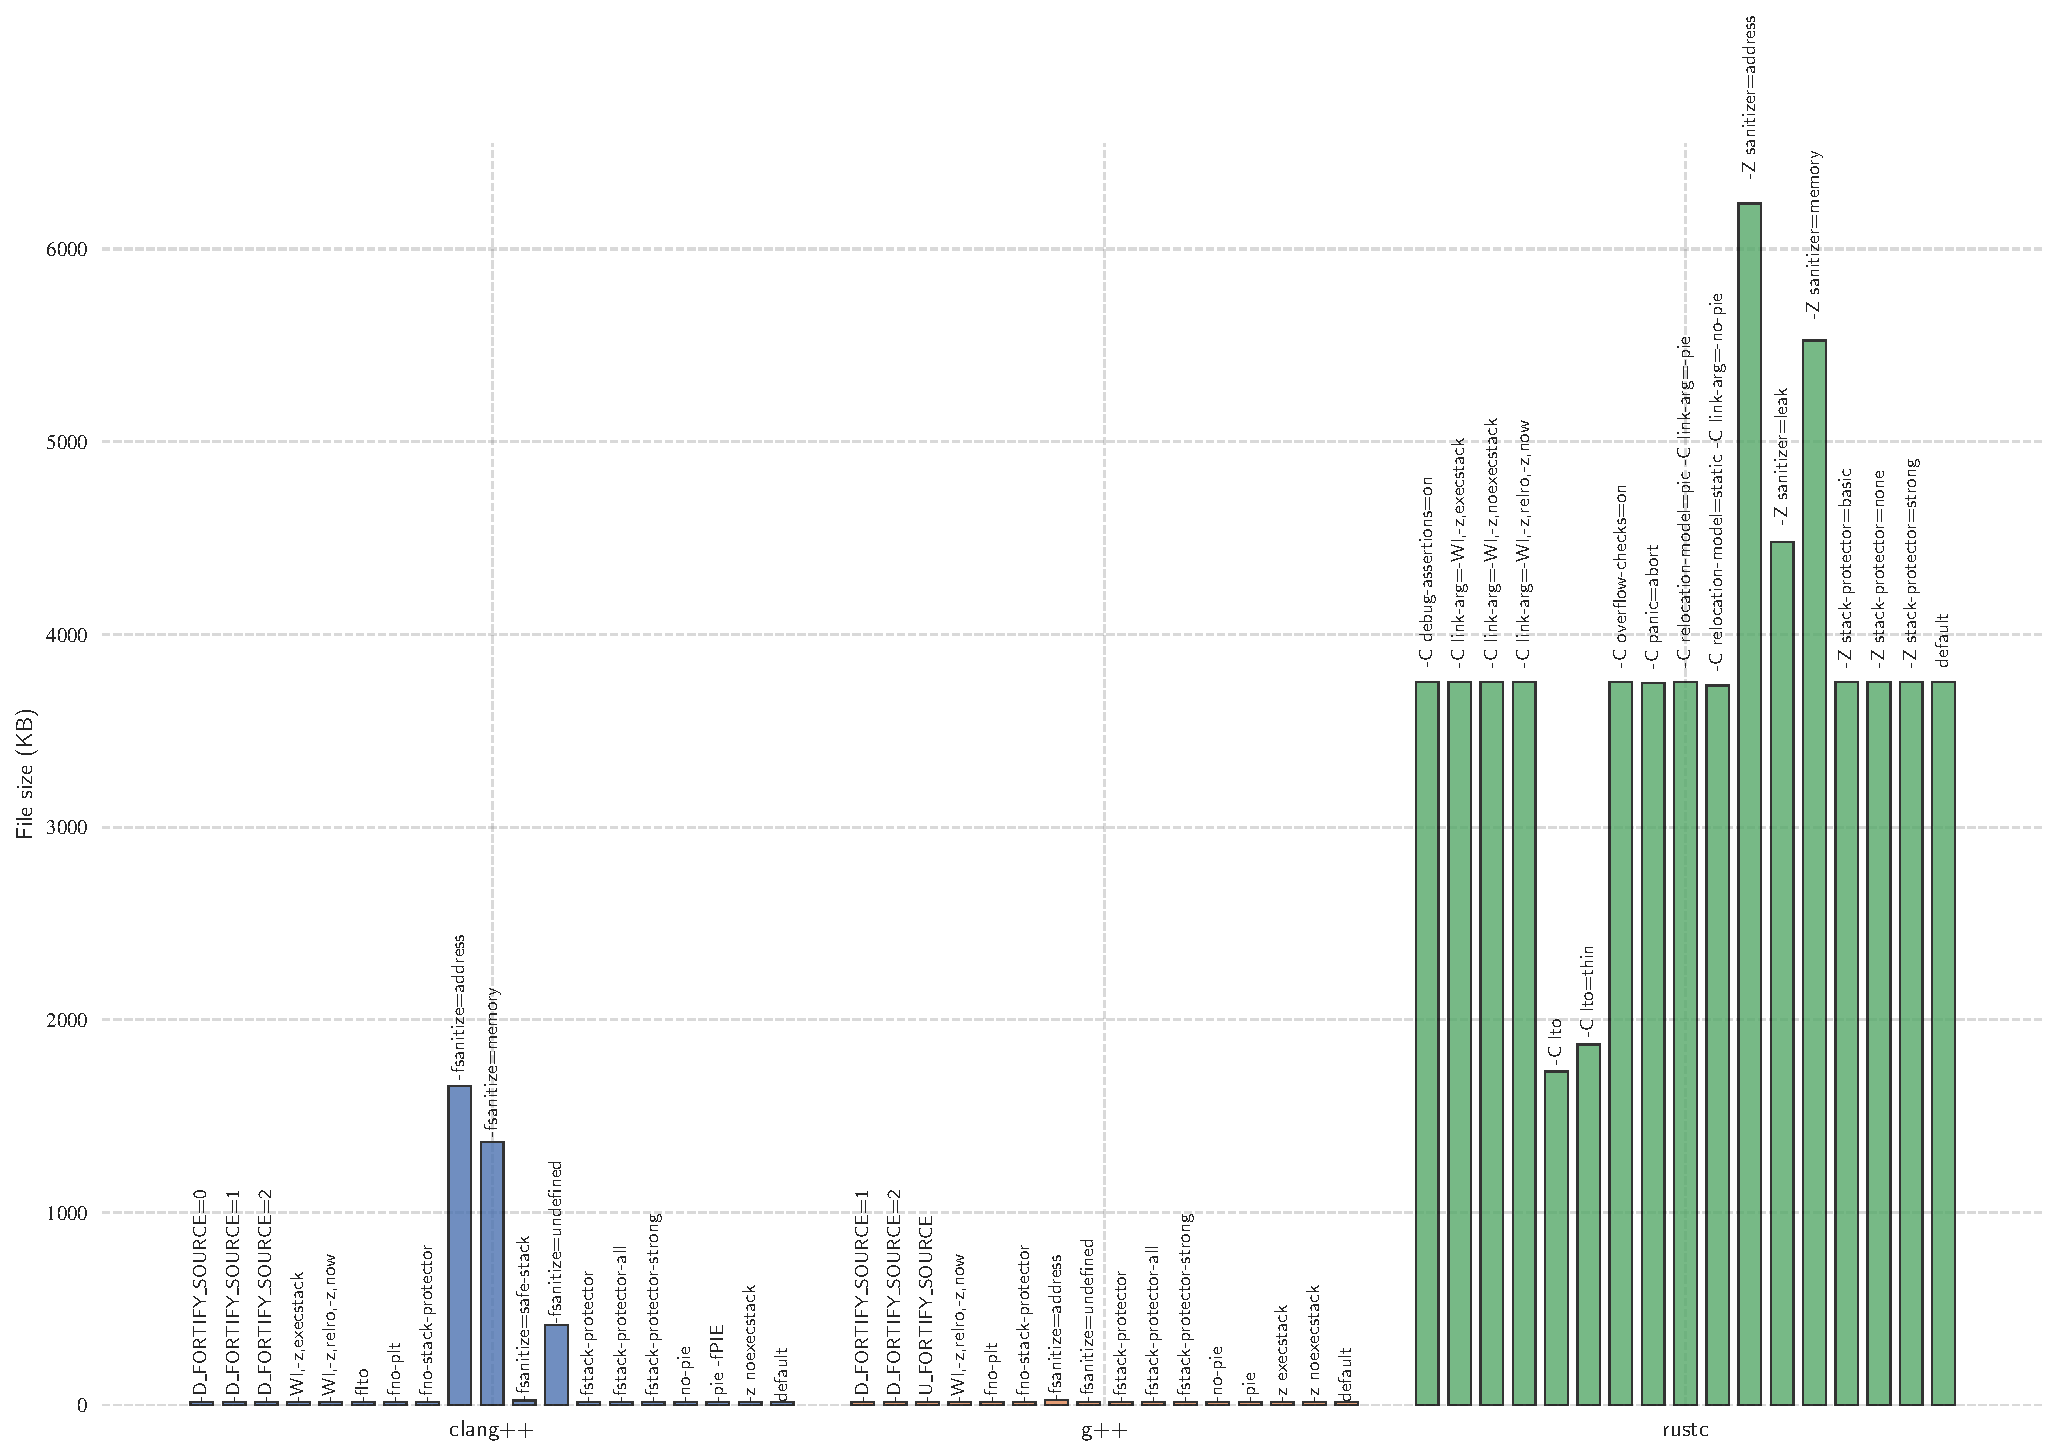
\includegraphics[width=\linewidth]{Gráficas/Gráficas_por_optimización/-O3/File_size_KB.pdf}
      \label{fig:Gráficas_gráficas_por_optimización__o3_file_size_kb}
    }
  \end{minipage}
  \hfill
  \begin{minipage}{0.48\textwidth}
    \centering
    \subfloat[Funciones fortificadas (\%)]{
      \includegraphics[width=\linewidth]{Gráficas/Gráficas_por_optimización/-O3/Fortified_Functions.pdf}
      \label{fig:Gráficas_gráficas_por_optimización__o3_fortified_functions}
    }
  \end{minipage}


  \vspace{1cm}

  \begin{minipage}{0.48\textwidth}
    \centering
    \subfloat[Uso de memoria (KB)]{
      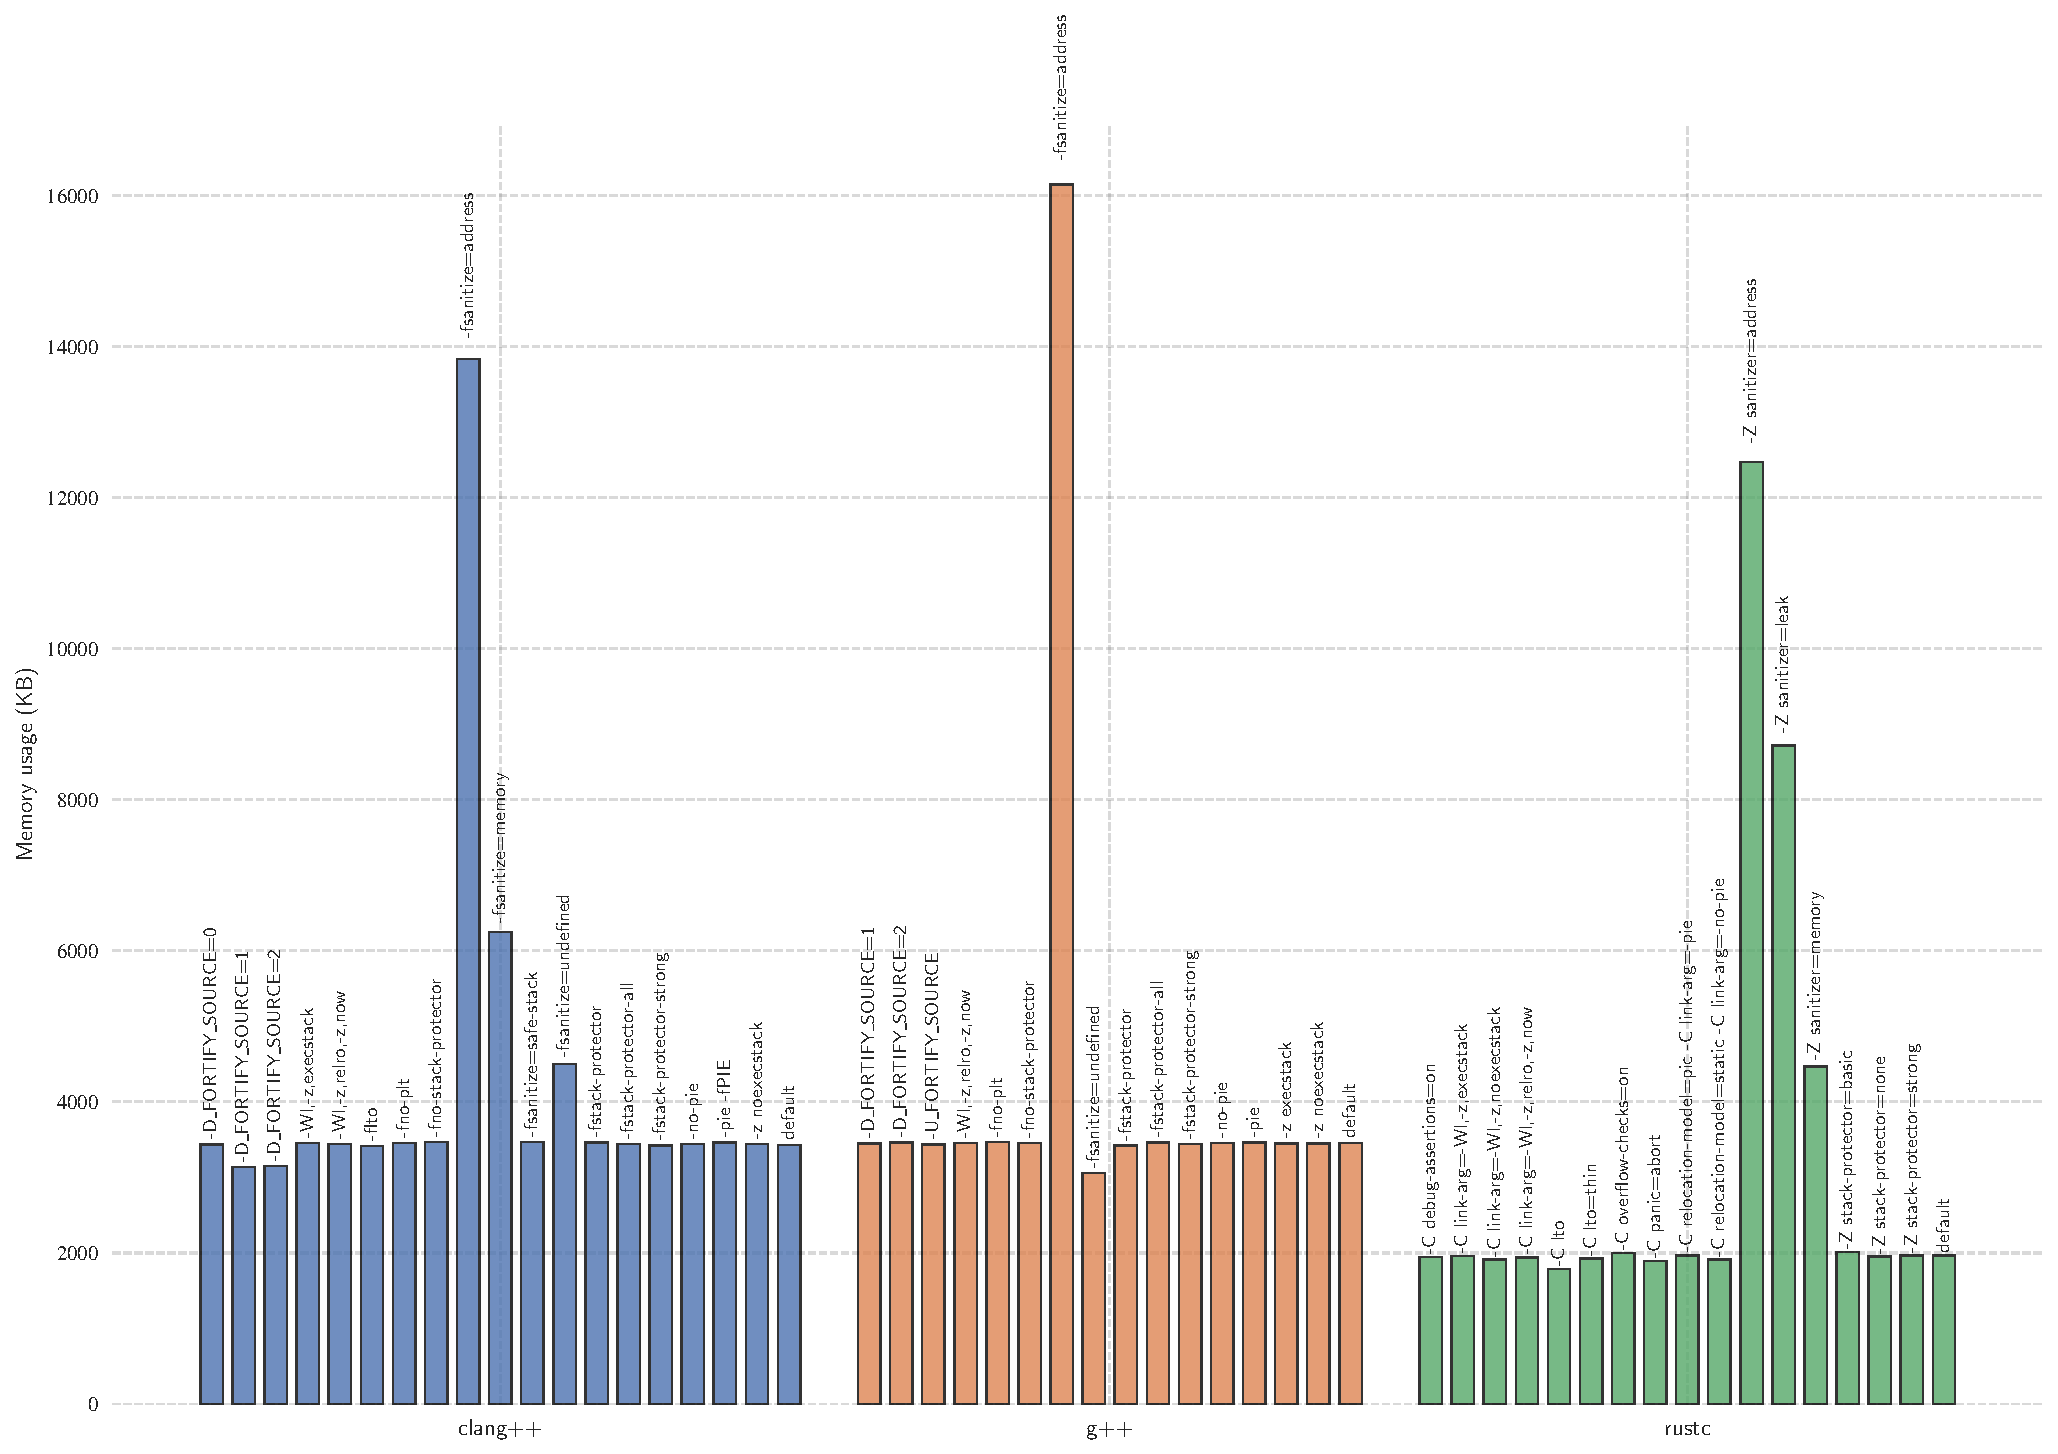
\includegraphics[width=\linewidth]{Gráficas/Gráficas_por_optimización/-O3/Memory_usage_KB.pdf}
      \label{fig:Gráficas_gráficas_por_optimización__o3_memory_usage_kb}
    }
  \end{minipage}
  \hfill
  \begin{minipage}{0.48\textwidth}
    \centering
    \subfloat[Tiempo (ms)]{
      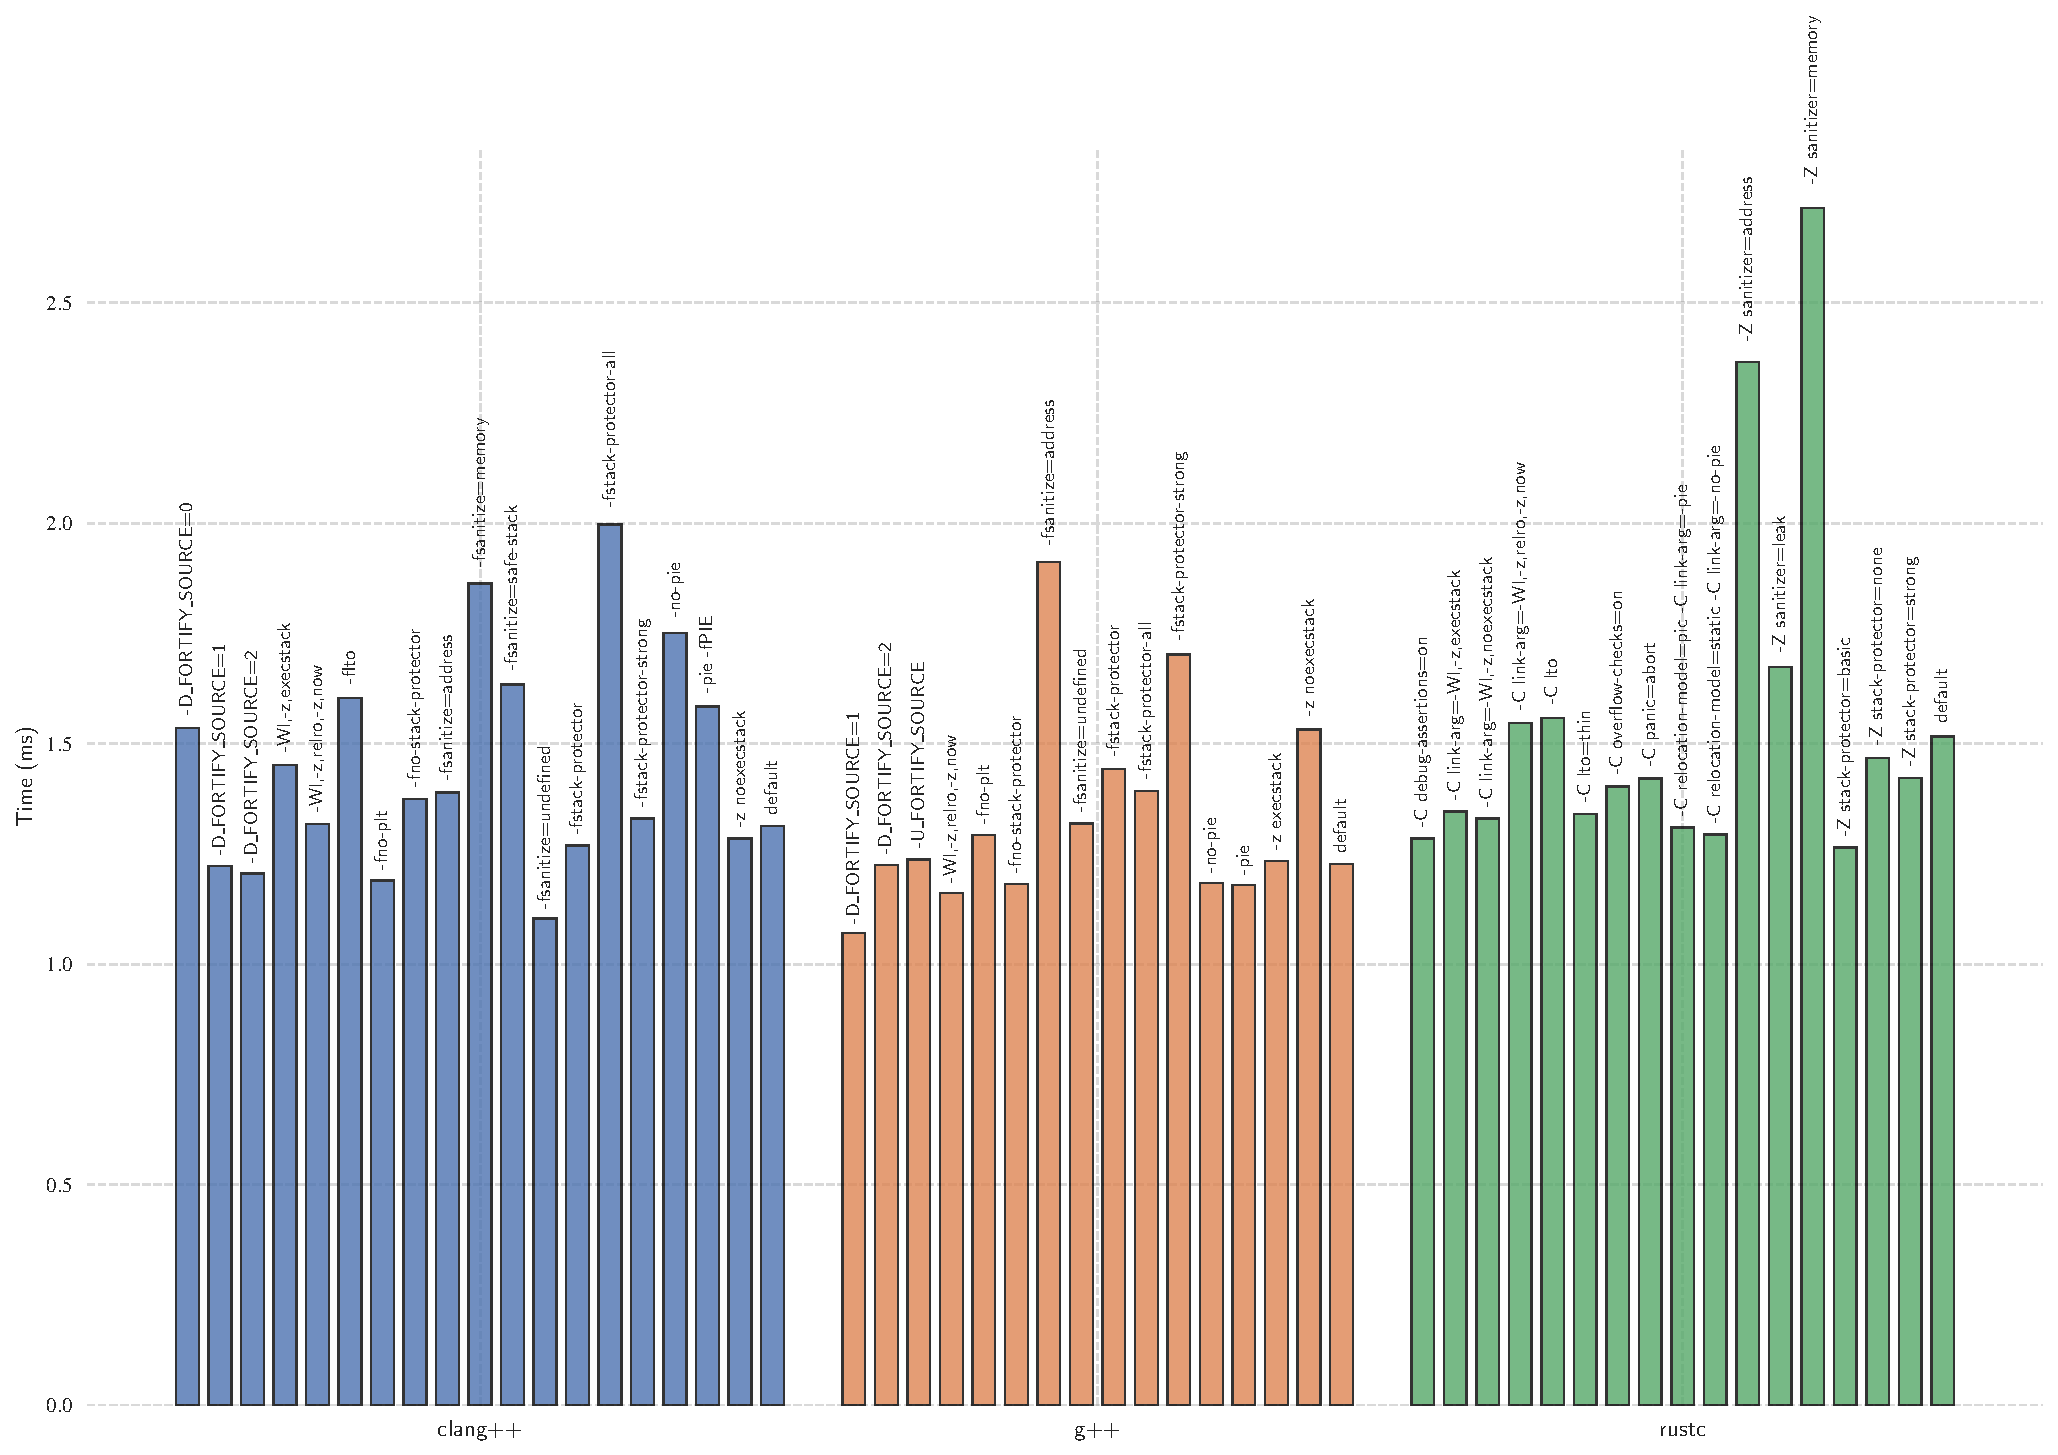
\includegraphics[width=\linewidth]{Gráficas/Gráficas_por_optimización/-O3/Time_ms.pdf}
      \label{fig:Gráficas_gráficas_por_optimización__o3_time_ms}
    }
  \end{minipage}

\end{figure}
\newpage

% === Gráficas_por_optimización/-Ofast ===
\subsection*{-OFAST}
\begin{figure}[htbp]
  \centering
  \caption{Resultados de compilación con optimización \texttt{-Ofast}}
  \vspace{0.5cm}

  \begin{minipage}{0.48\textwidth}
    \centering
    \subfloat[Tamaño del archivo (KB)]{
      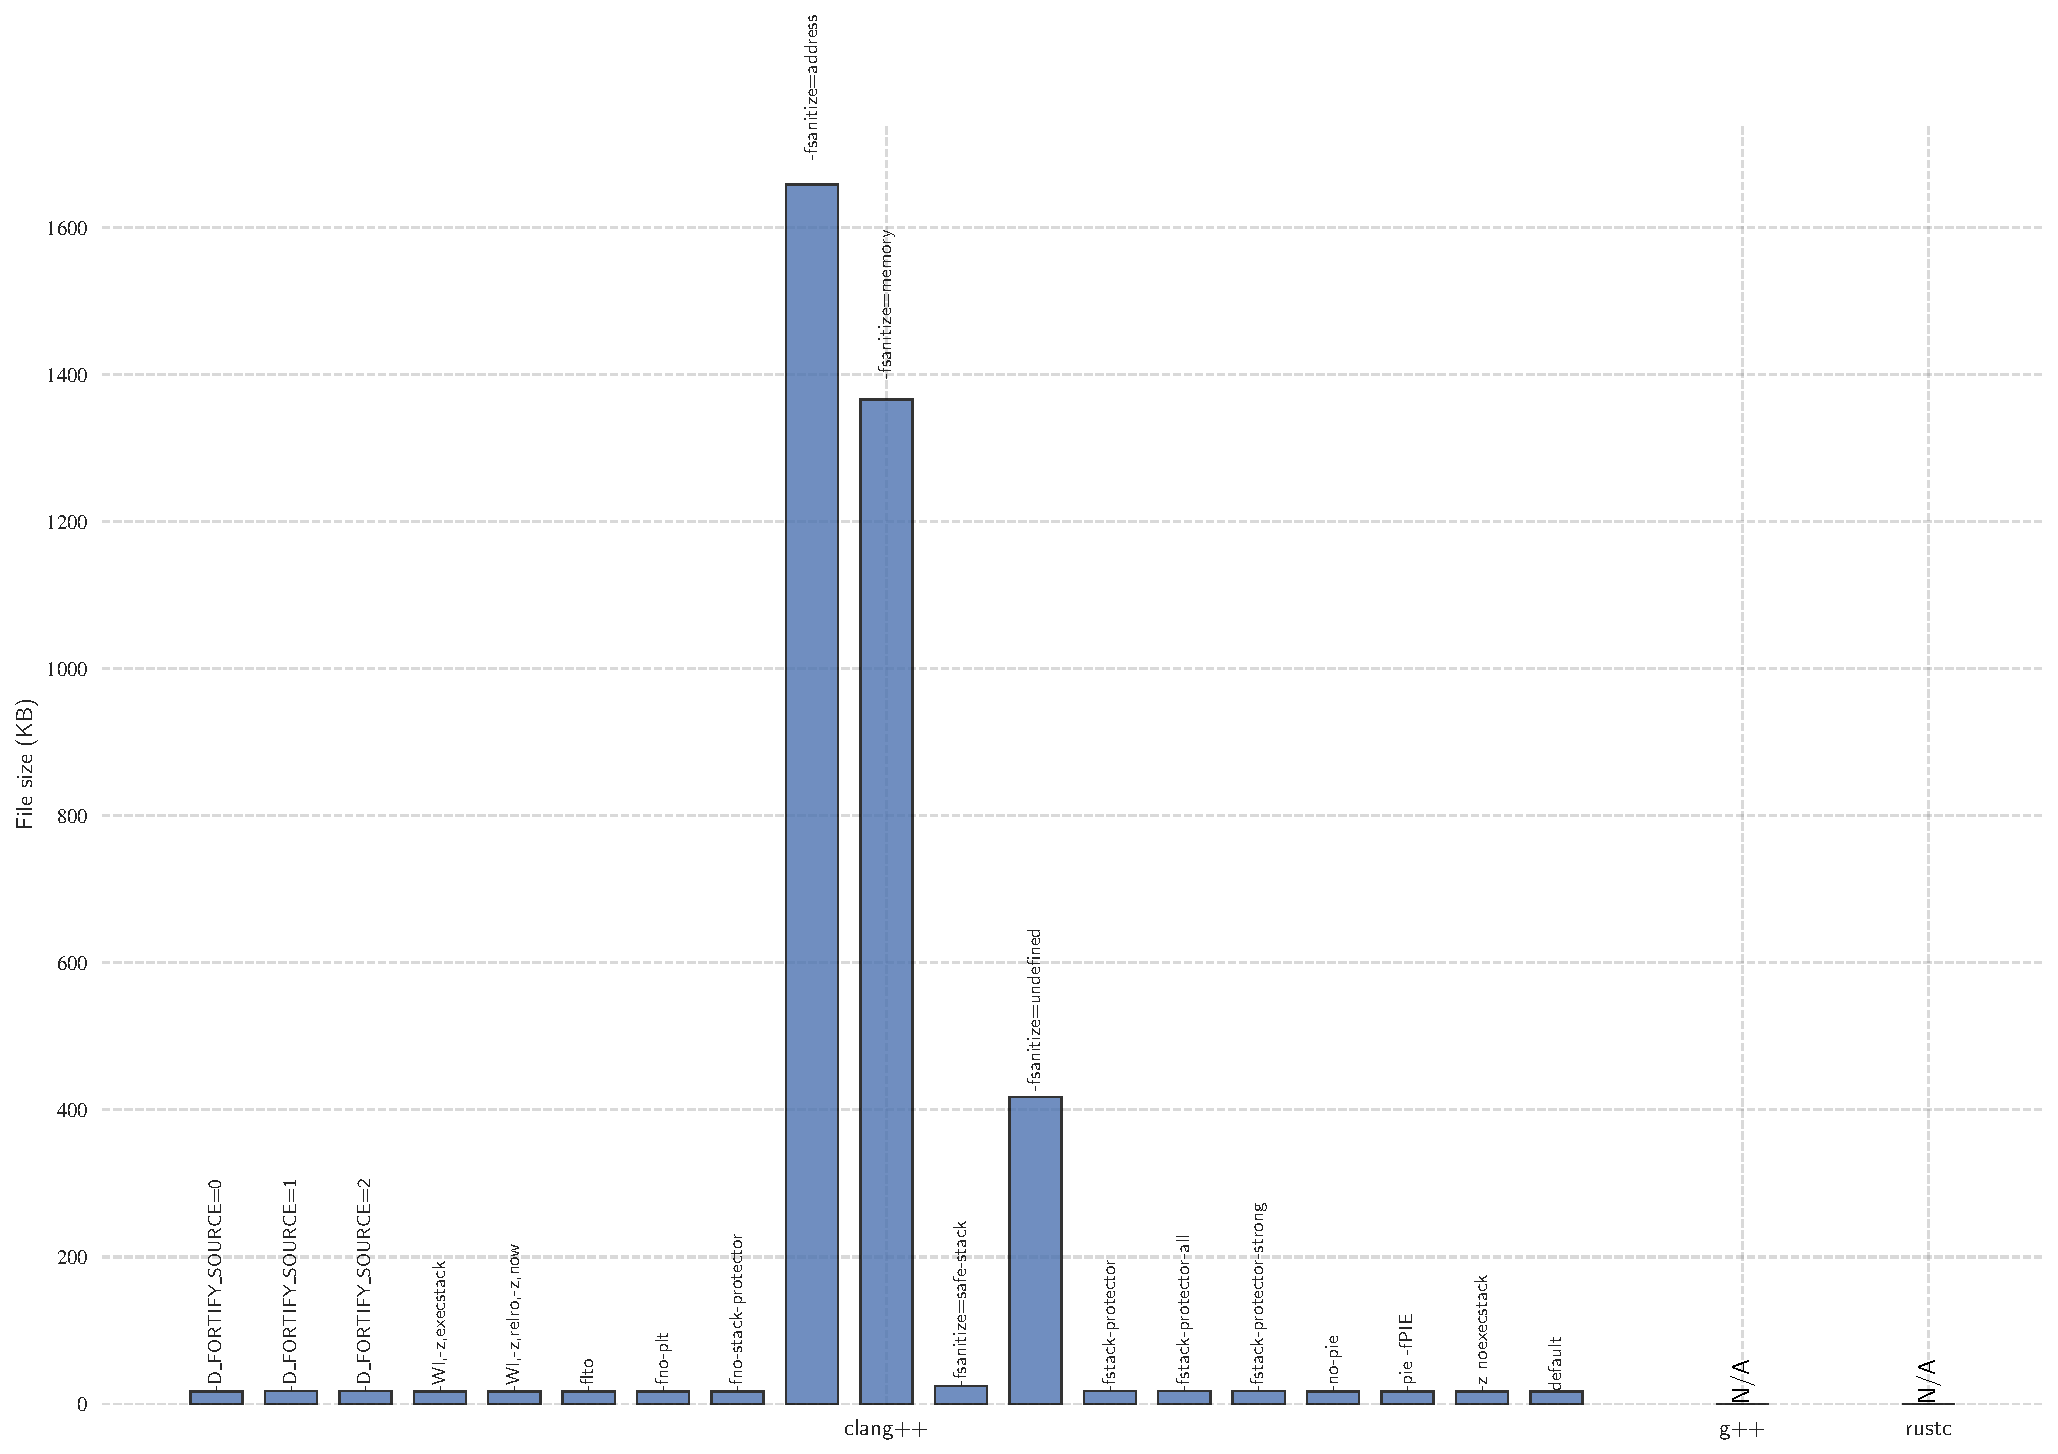
\includegraphics[width=\linewidth]{Gráficas/Gráficas_por_optimización/-Ofast/File_size_KB.pdf}
      \label{fig:Gráficas_gráficas_por_optimización__ofast_file_size_kb}
    }
  \end{minipage}
  \hfill
  \begin{minipage}{0.48\textwidth}
    \centering
    \subfloat[Funciones fortificadas (\%)]{
      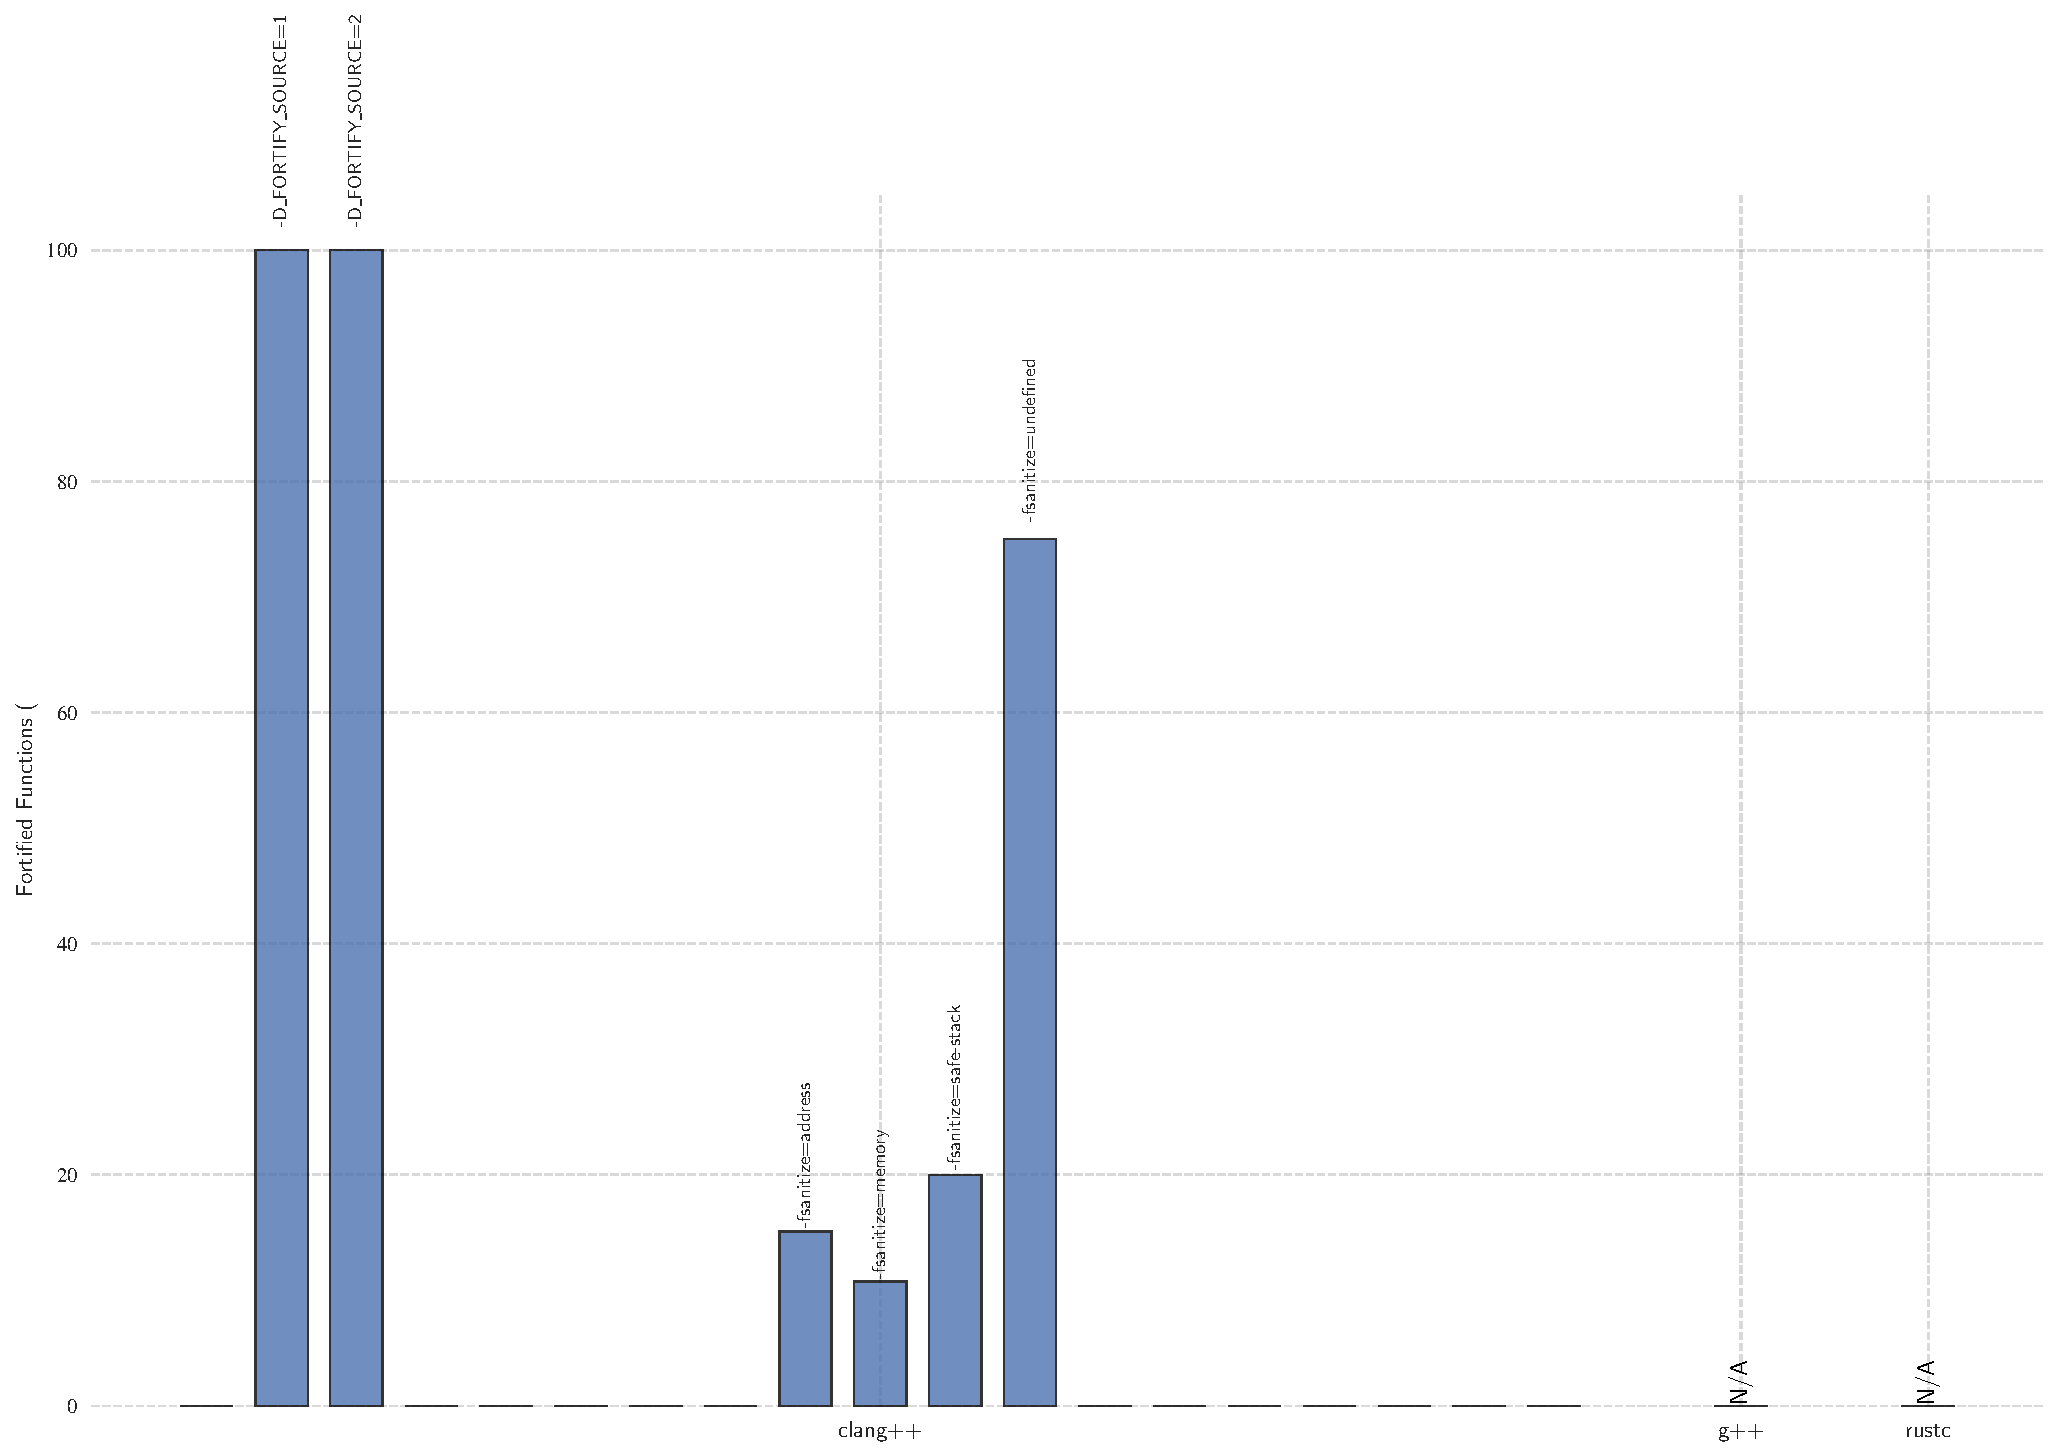
\includegraphics[width=\linewidth]{Gráficas/Gráficas_por_optimización/-Ofast/Fortified_Functions.pdf}
      \label{fig:Gráficas_gráficas_por_optimización__ofast_fortified_functions}
    }
  \end{minipage}


  \vspace{1cm}

  \begin{minipage}{0.48\textwidth}
    \centering
    \subfloat[Uso de memoria (KB)]{
      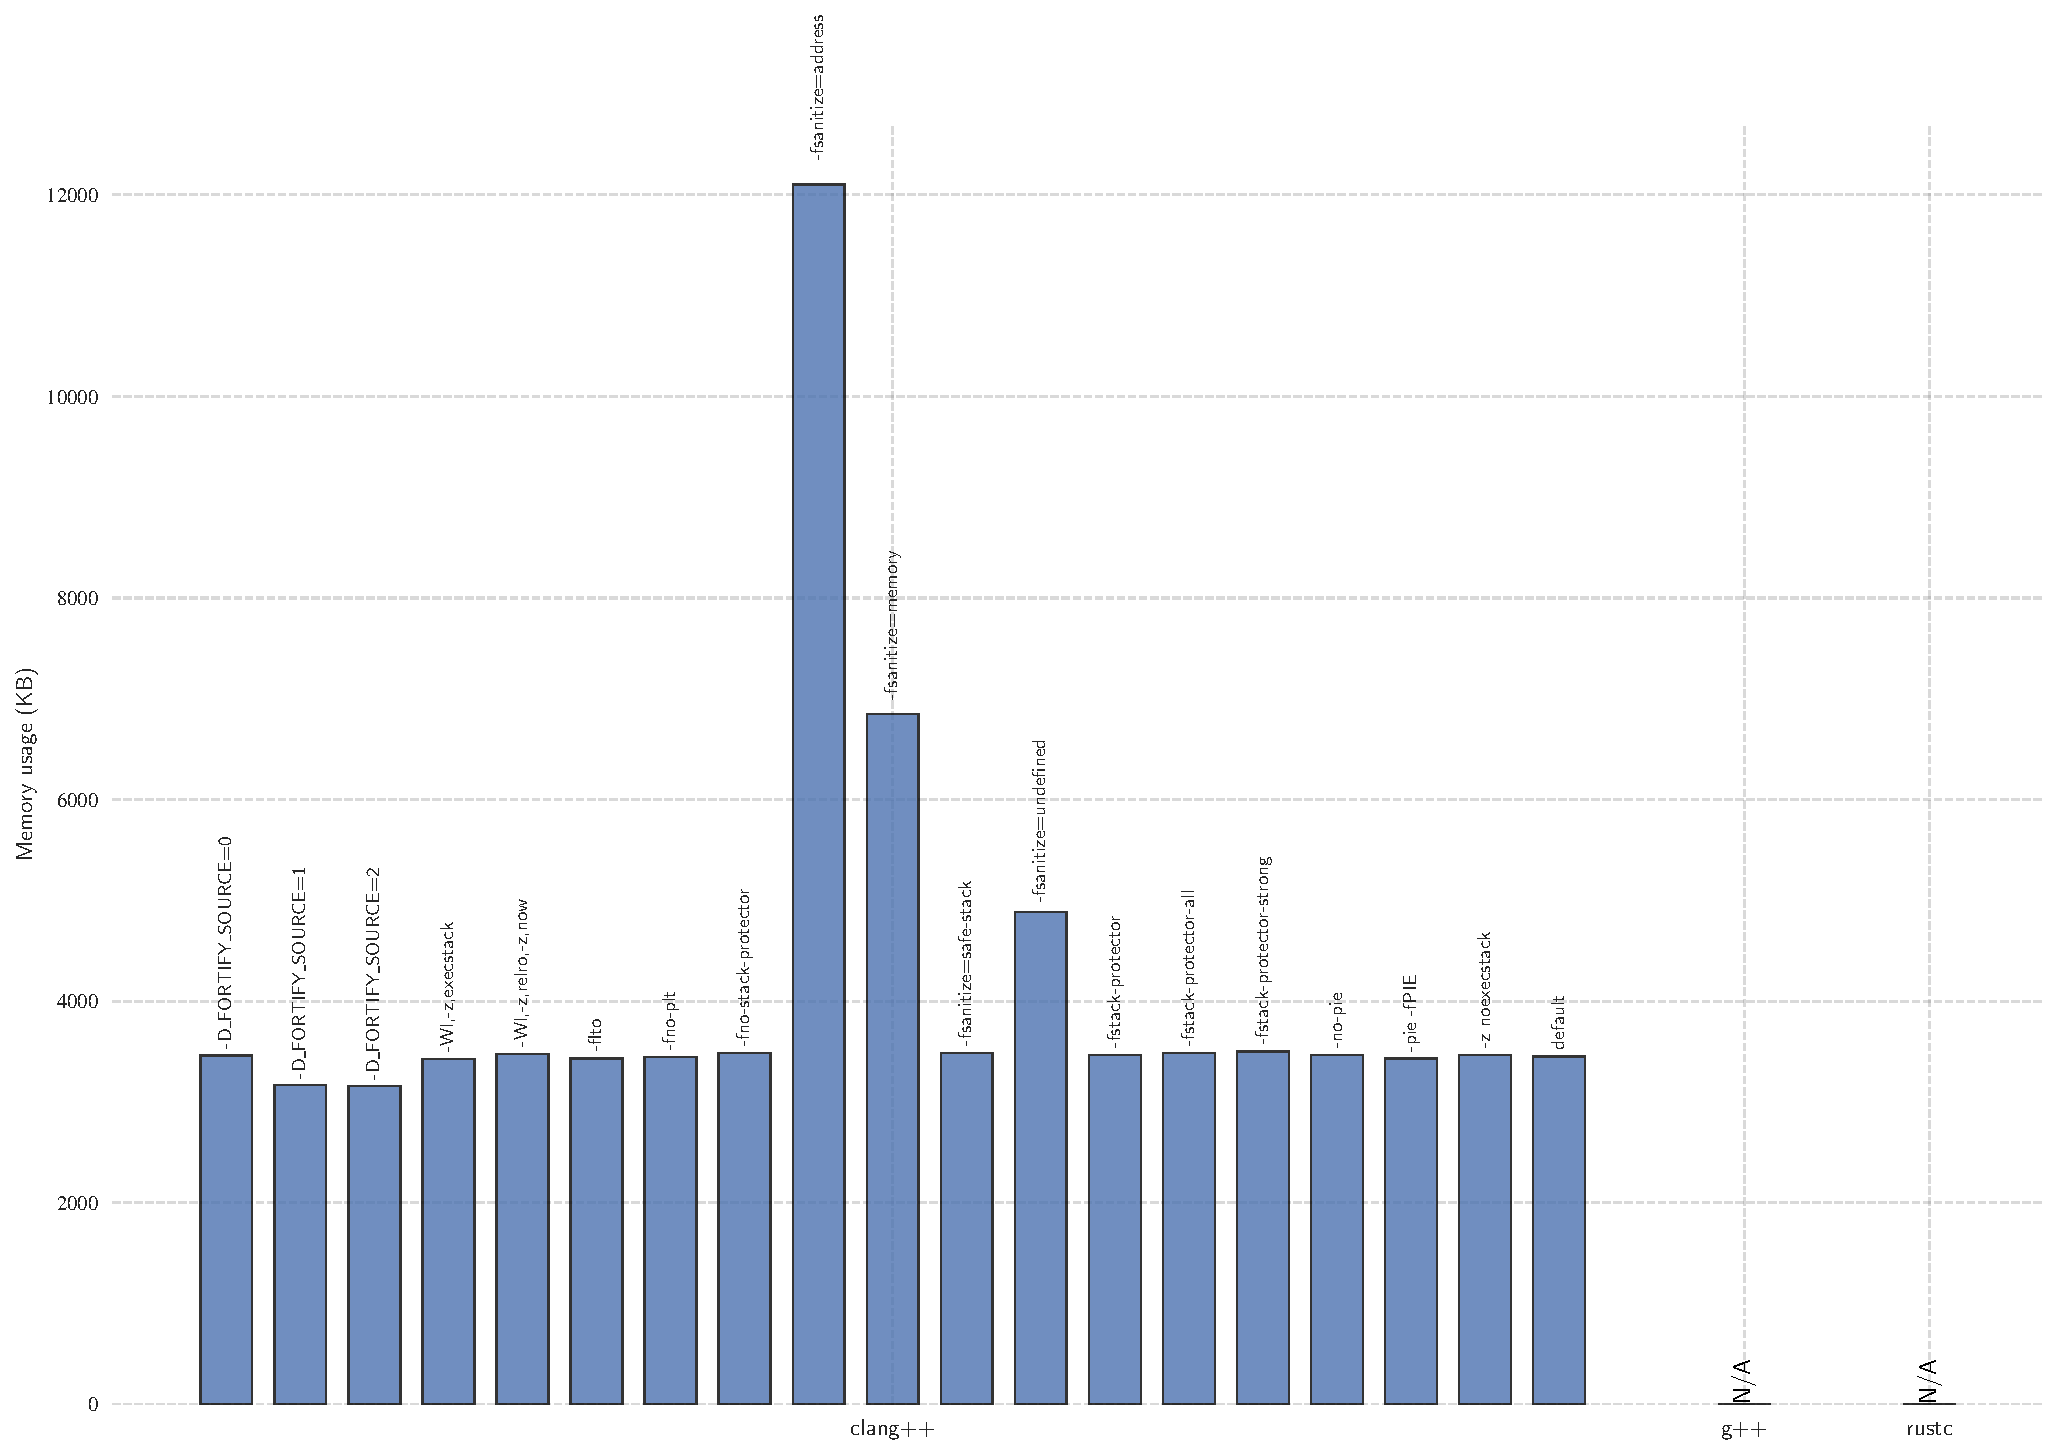
\includegraphics[width=\linewidth]{Gráficas/Gráficas_por_optimización/-Ofast/Memory_usage_KB.pdf}
      \label{fig:Gráficas_gráficas_por_optimización__ofast_memory_usage_kb}
    }
  \end{minipage}
  \hfill
  \begin{minipage}{0.48\textwidth}
    \centering
    \subfloat[Tiempo (ms)]{
      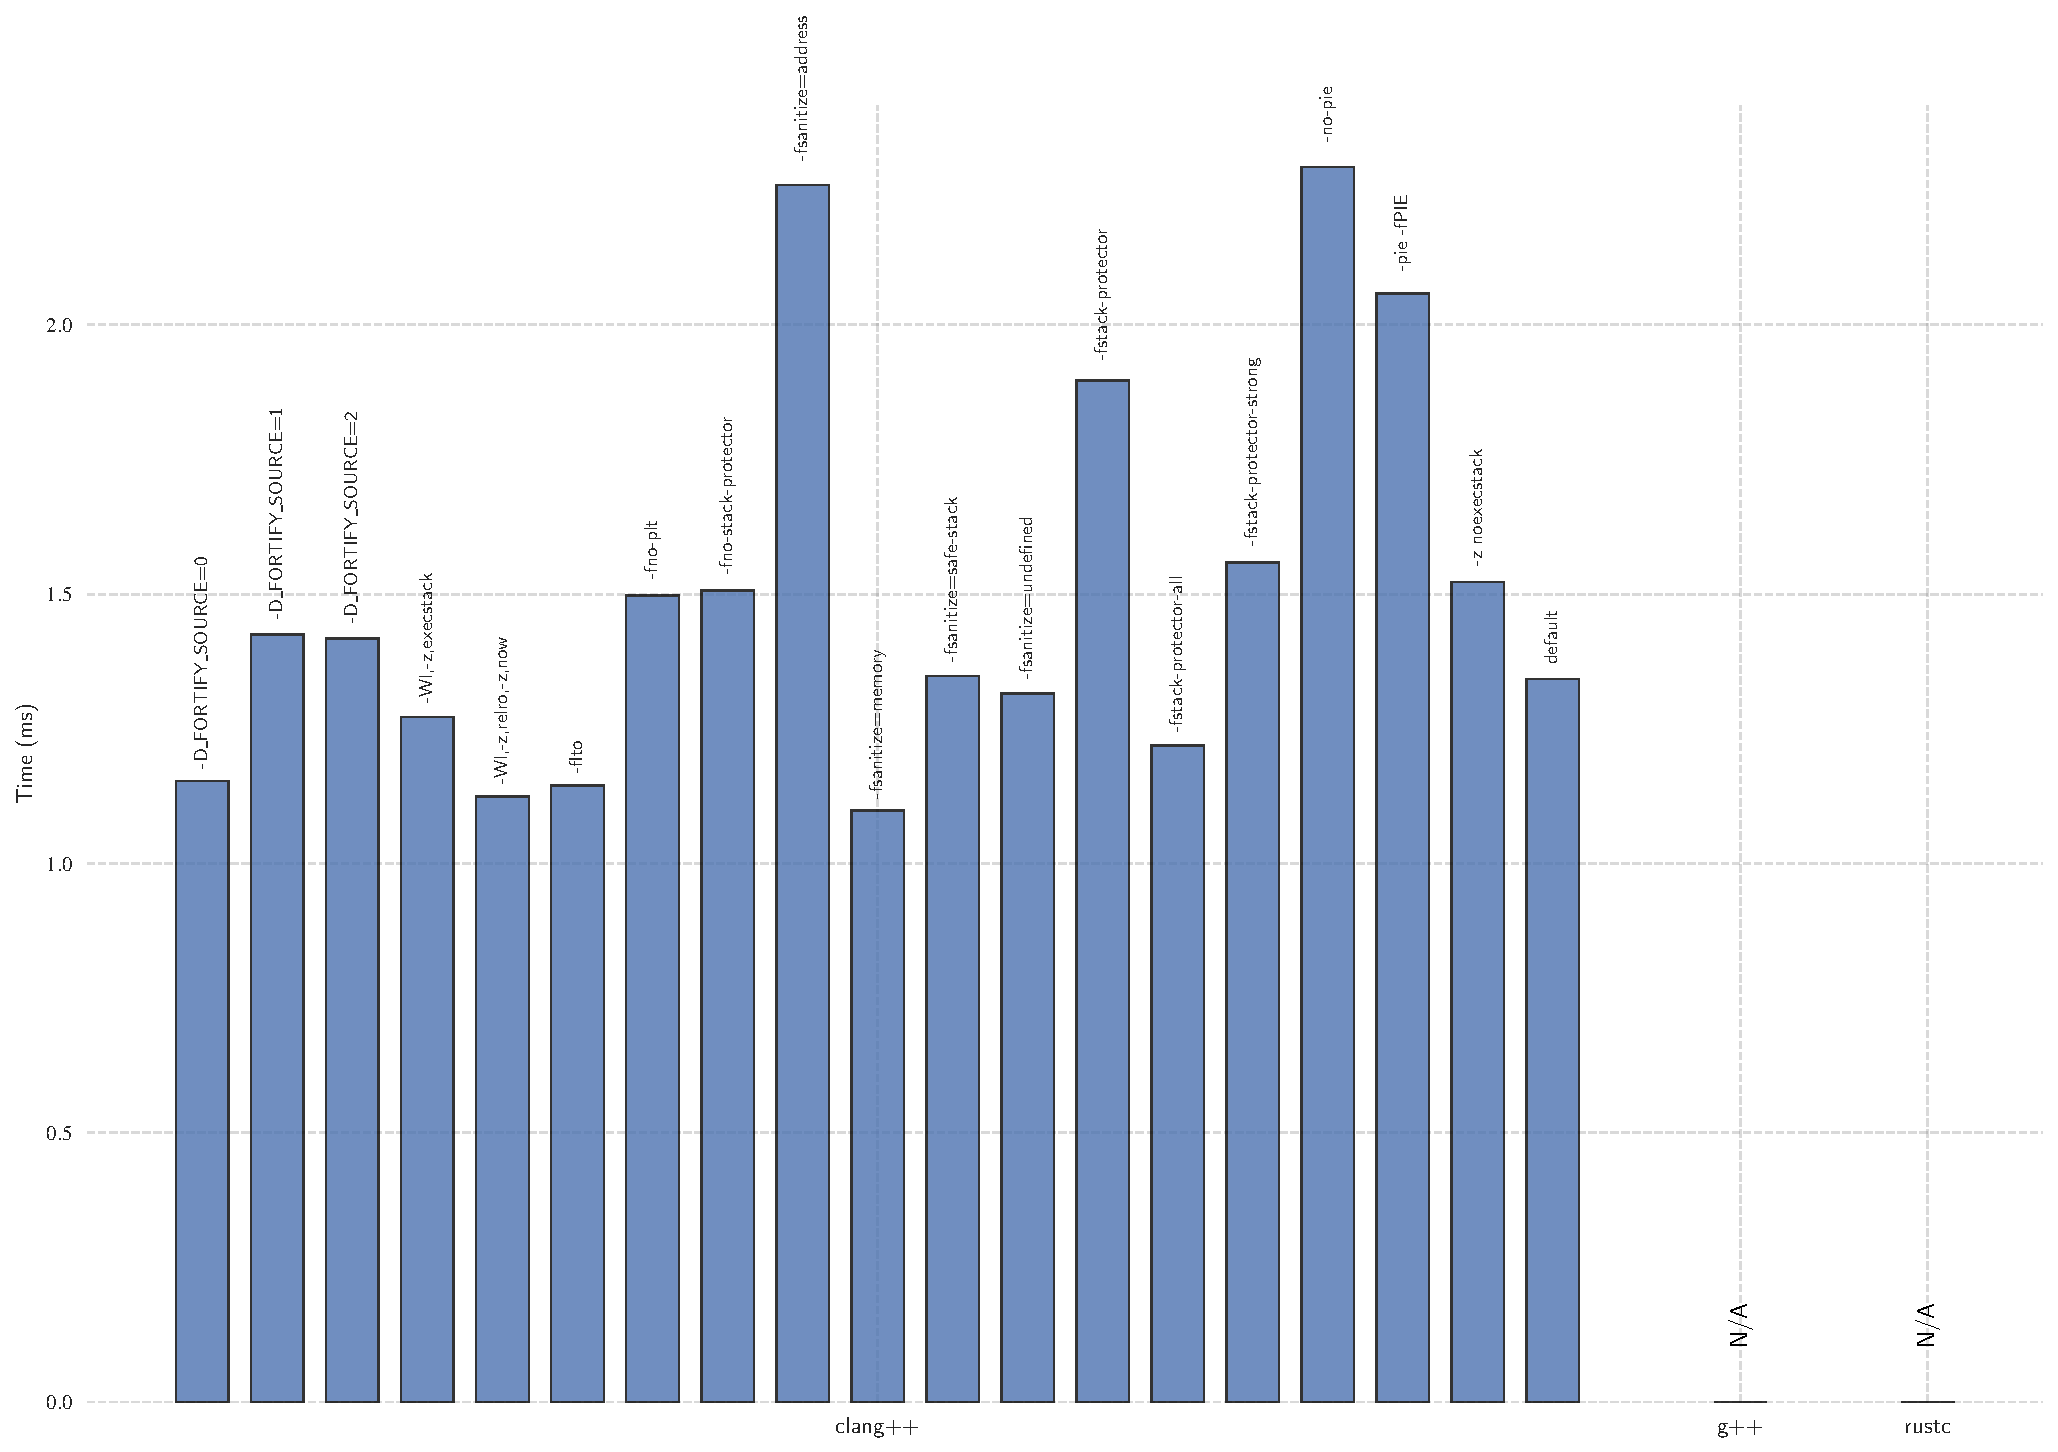
\includegraphics[width=\linewidth]{Gráficas/Gráficas_por_optimización/-Ofast/Time_ms.pdf}
      \label{fig:Gráficas_gráficas_por_optimización__ofast_time_ms}
    }
  \end{minipage}

\end{figure}
\newpage

% === Gráficas_por_optimización/-Os ===
\subsection*{-OS}
\begin{figure}[htbp]
  \centering
  \caption{Resultados de compilación con optimización \texttt{-Os}}
  \vspace{0.5cm}

  \begin{minipage}{0.48\textwidth}
    \centering
    \subfloat[Tamaño del archivo (KB)]{
      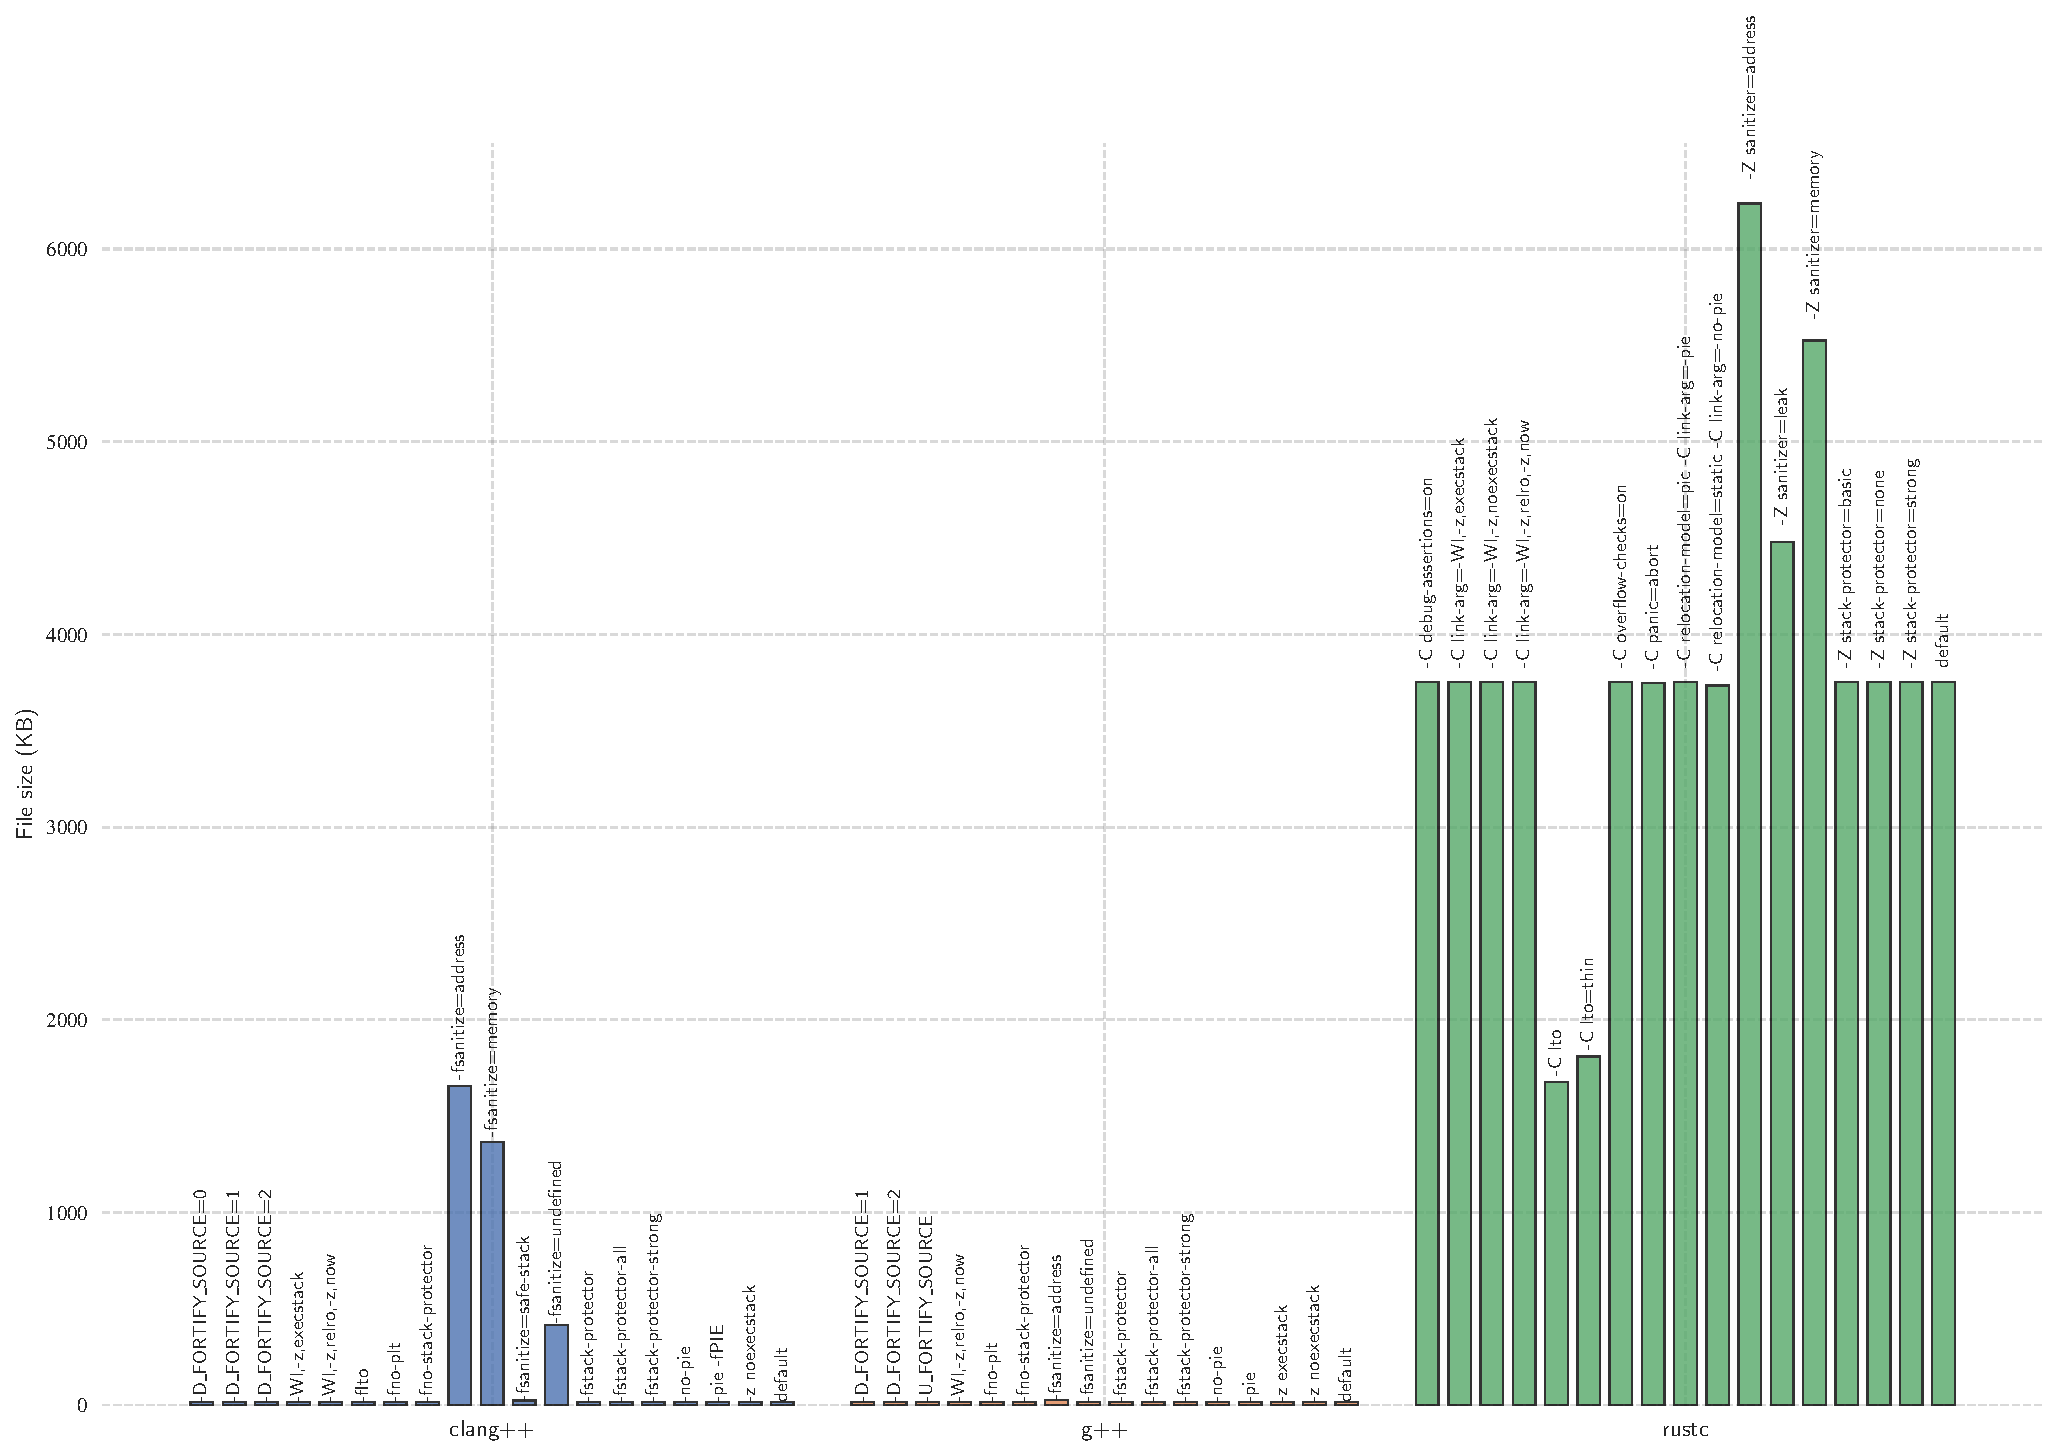
\includegraphics[width=\linewidth]{Gráficas/Gráficas_por_optimización/-Os/File_size_KB.pdf}
      \label{fig:Gráficas_gráficas_por_optimización__os_file_size_kb}
    }
  \end{minipage}
  \hfill
  \begin{minipage}{0.48\textwidth}
    \centering
    \subfloat[Funciones fortificadas (\%)]{
      \includegraphics[width=\linewidth]{Gráficas/Gráficas_por_optimización/-Os/Fortified_Functions.pdf}
      \label{fig:Gráficas_gráficas_por_optimización__os_fortified_functions}
    }
  \end{minipage}


  \vspace{1cm}

  \begin{minipage}{0.48\textwidth}
    \centering
    \subfloat[Uso de memoria (KB)]{
      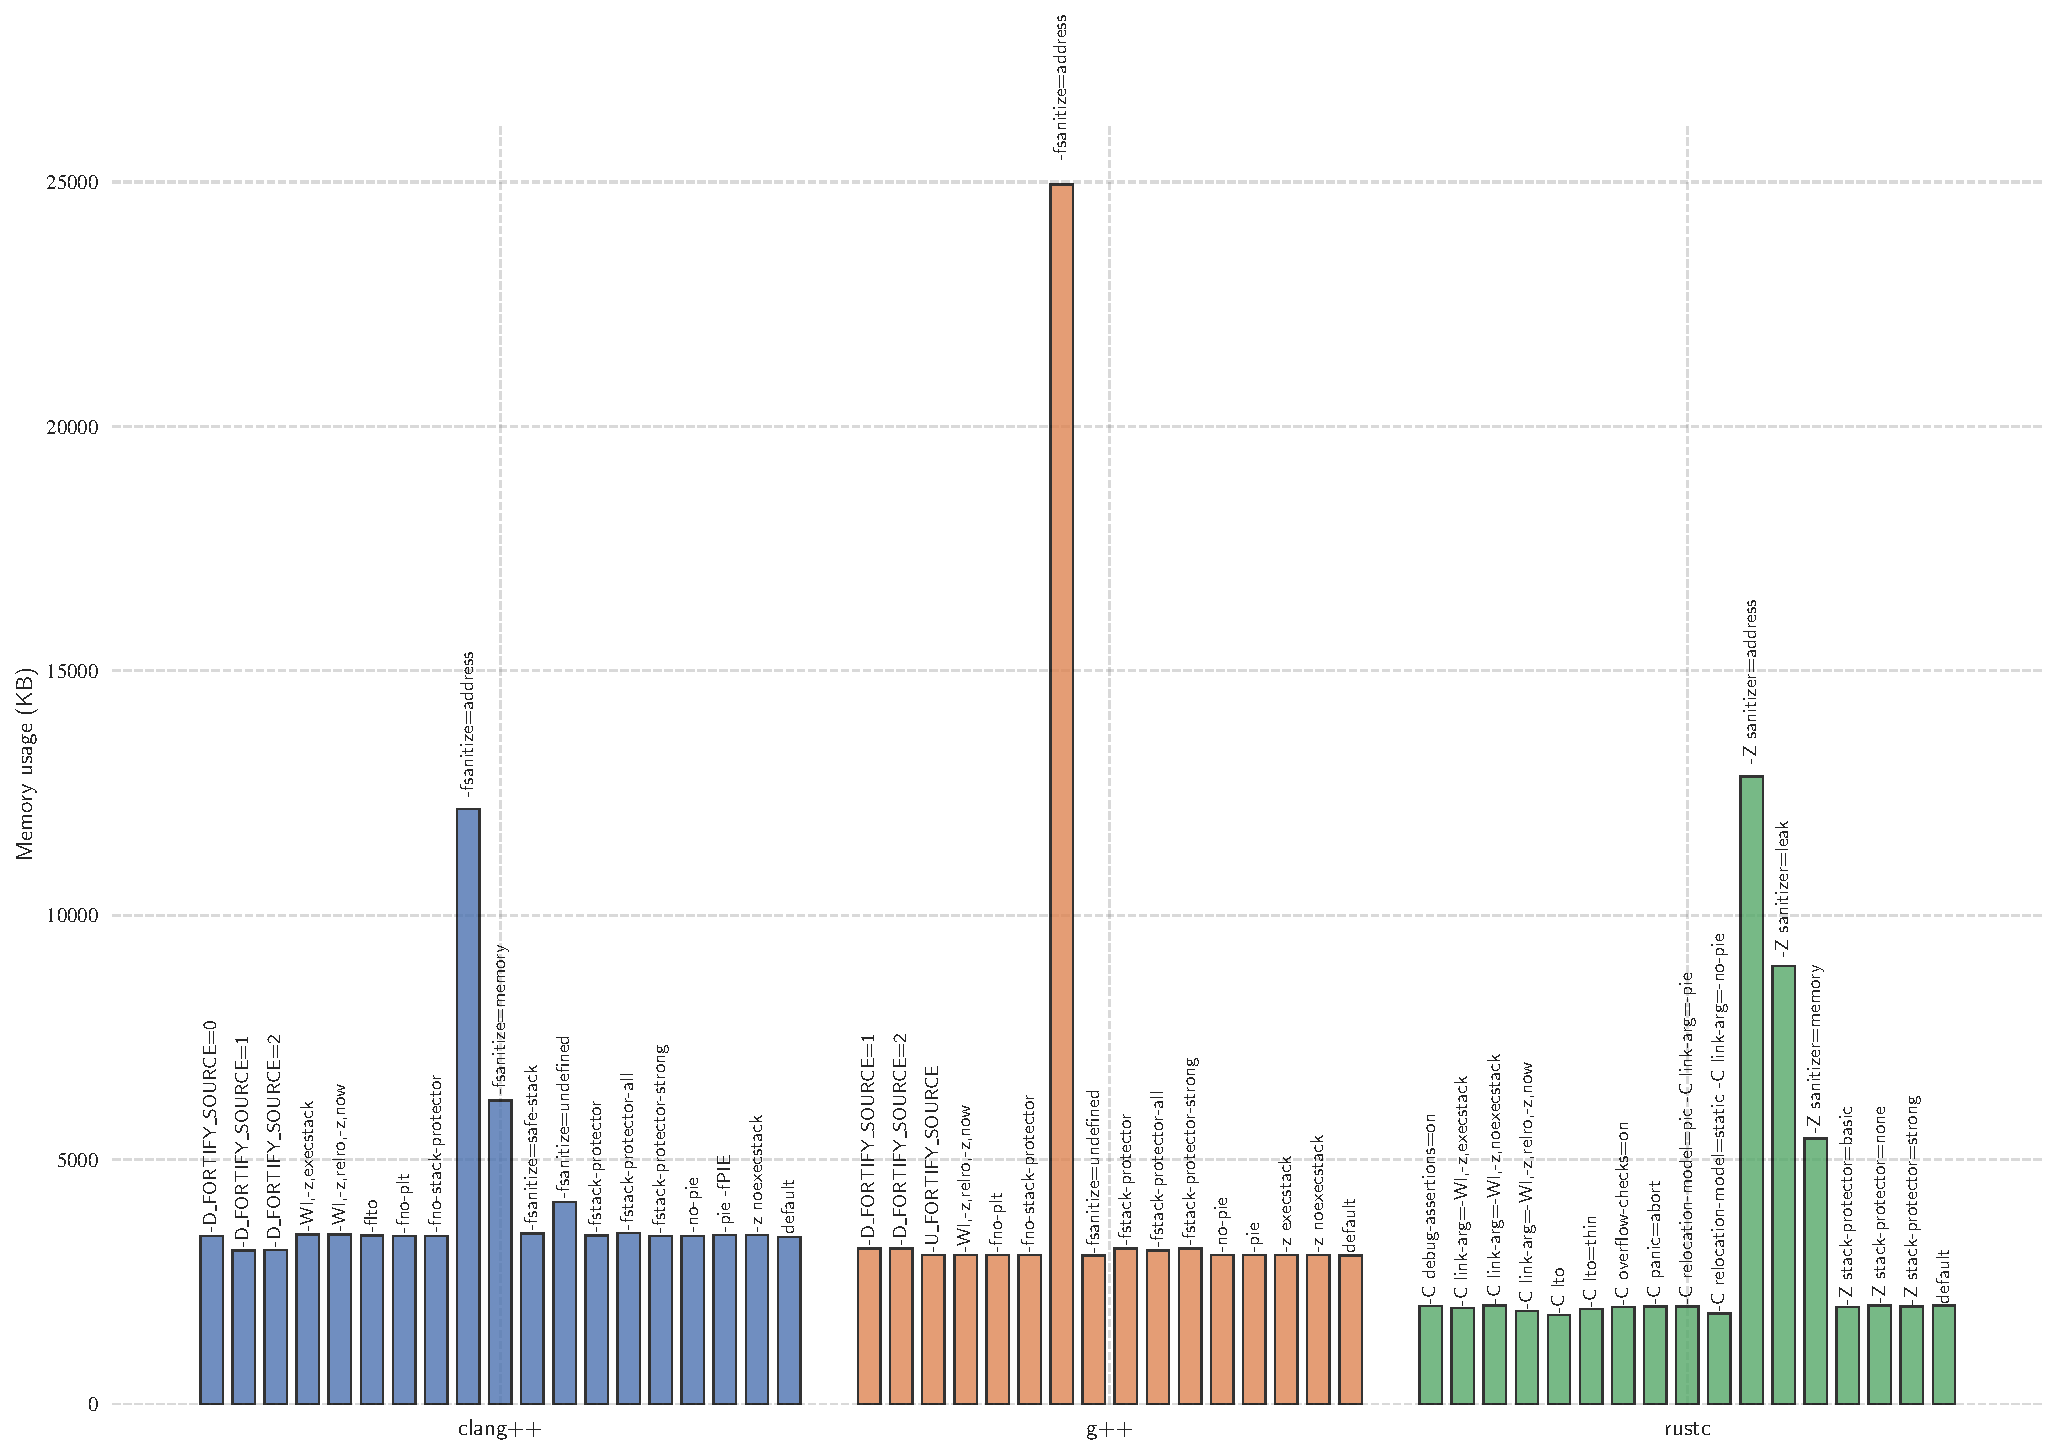
\includegraphics[width=\linewidth]{Gráficas/Gráficas_por_optimización/-Os/Memory_usage_KB.pdf}
      \label{fig:Gráficas_gráficas_por_optimización__os_memory_usage_kb}
    }
  \end{minipage}
  \hfill
  \begin{minipage}{0.48\textwidth}
    \centering
    \subfloat[Tiempo (ms)]{
      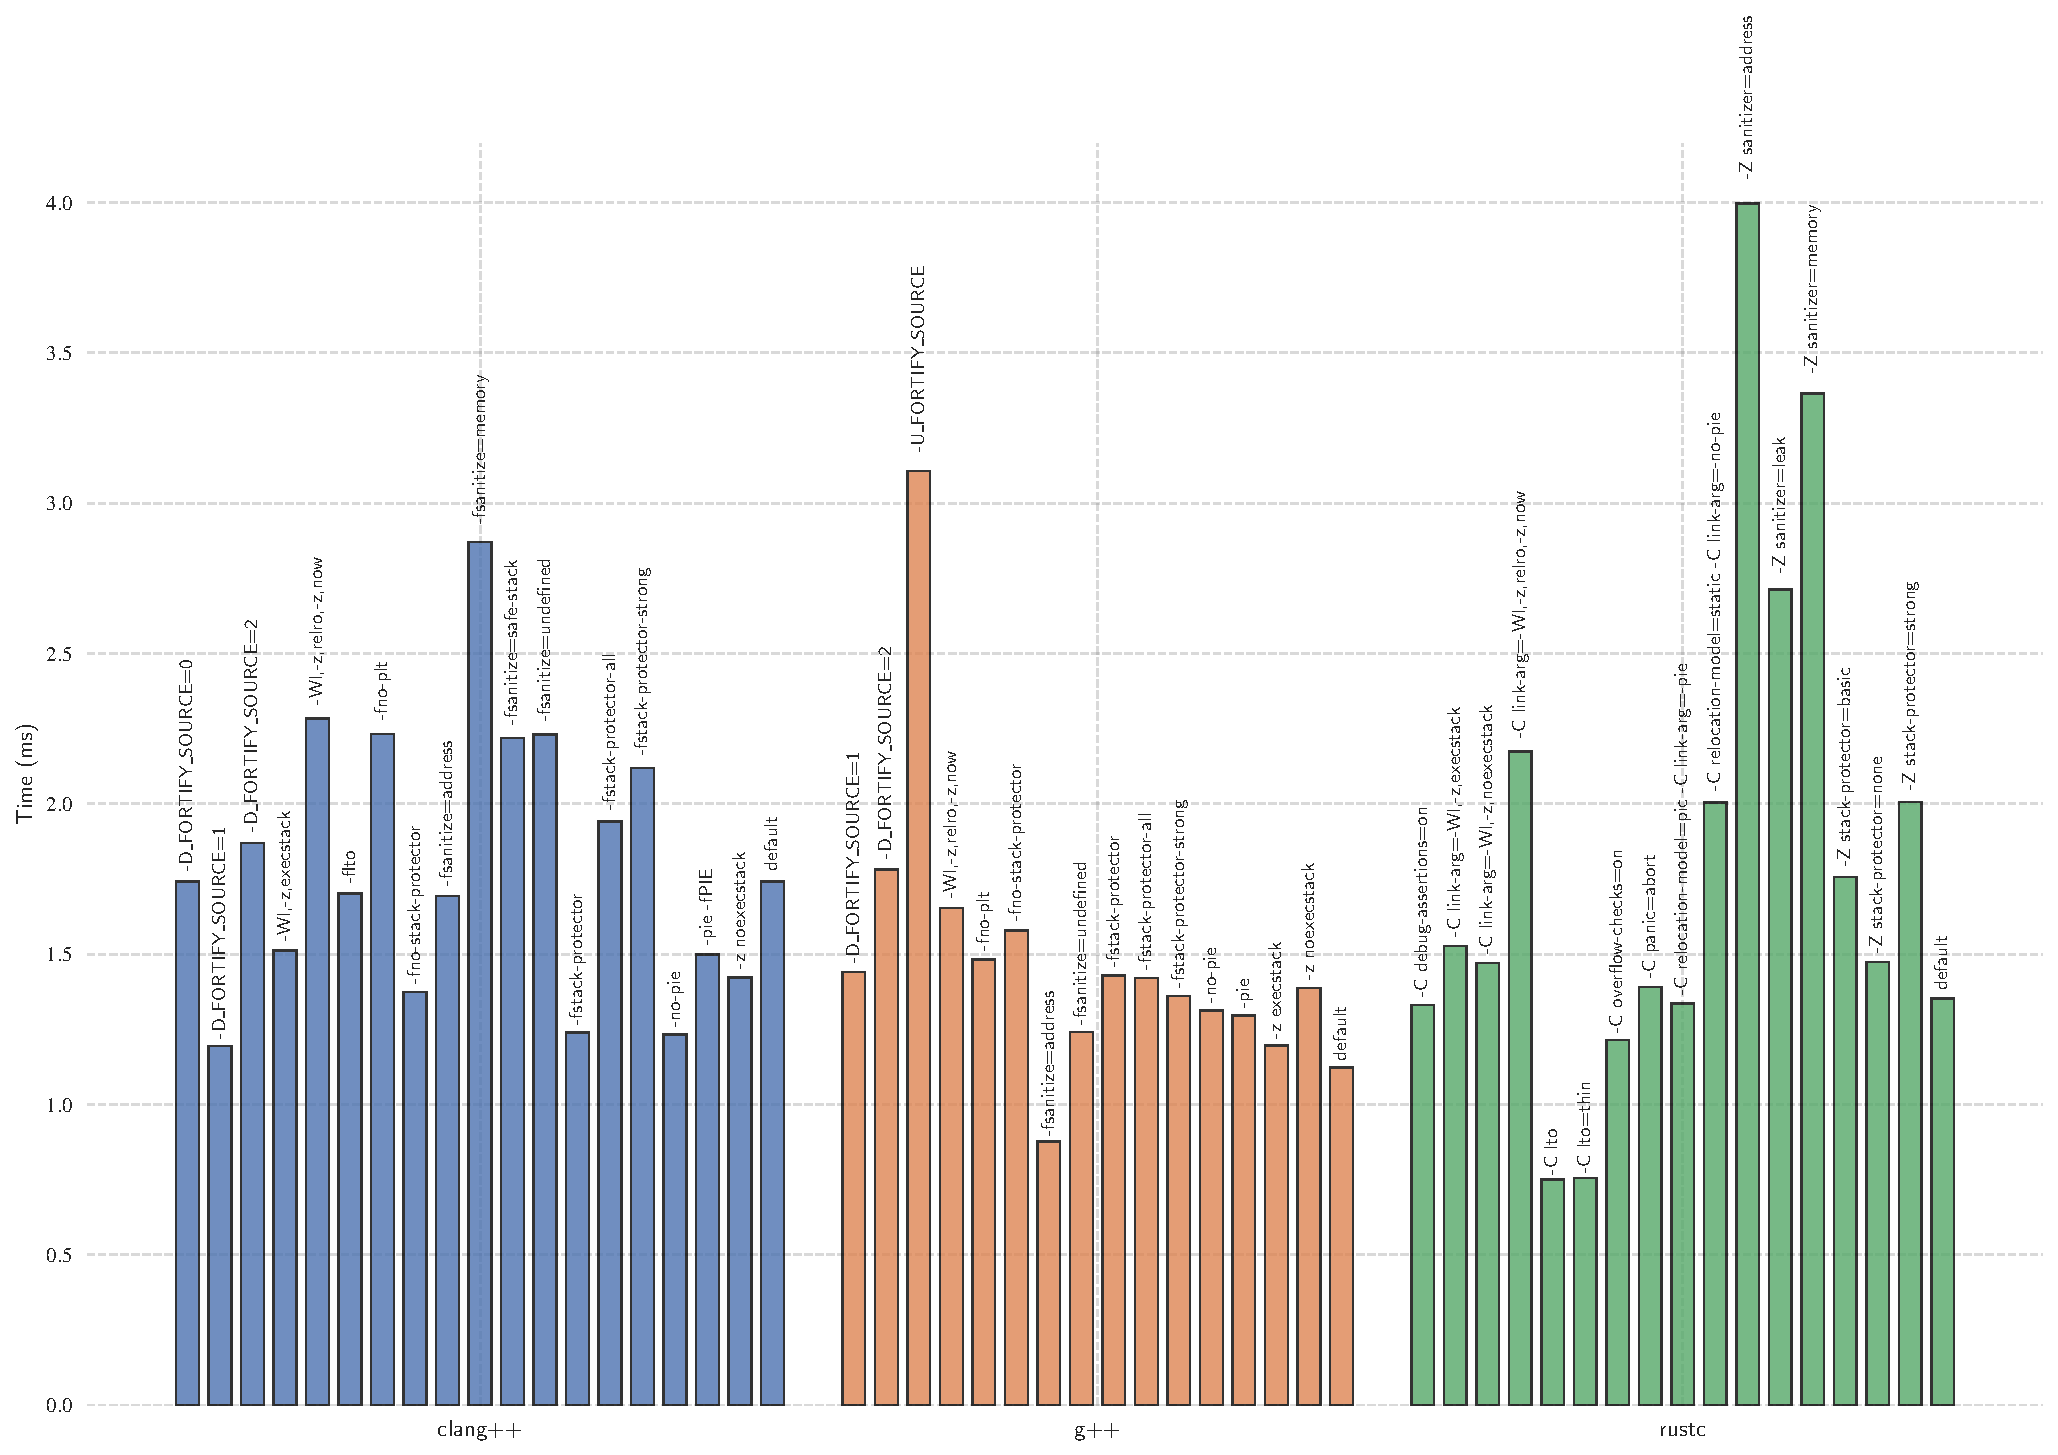
\includegraphics[width=\linewidth]{Gráficas/Gráficas_por_optimización/-Os/Time_ms.pdf}
      \label{fig:Gráficas_gráficas_por_optimización__os_time_ms}
    }
  \end{minipage}

\end{figure}
\newpage

% === Gráficas_por_optimización/-Oz ===
\subsection*{-OZ}
\begin{figure}[htbp]
  \centering
  \caption{Resultados de compilación con optimización \texttt{-Oz}}
  \vspace{0.5cm}

  \begin{minipage}{0.48\textwidth}
    \centering
    \subfloat[Tamaño del archivo (KB)]{
      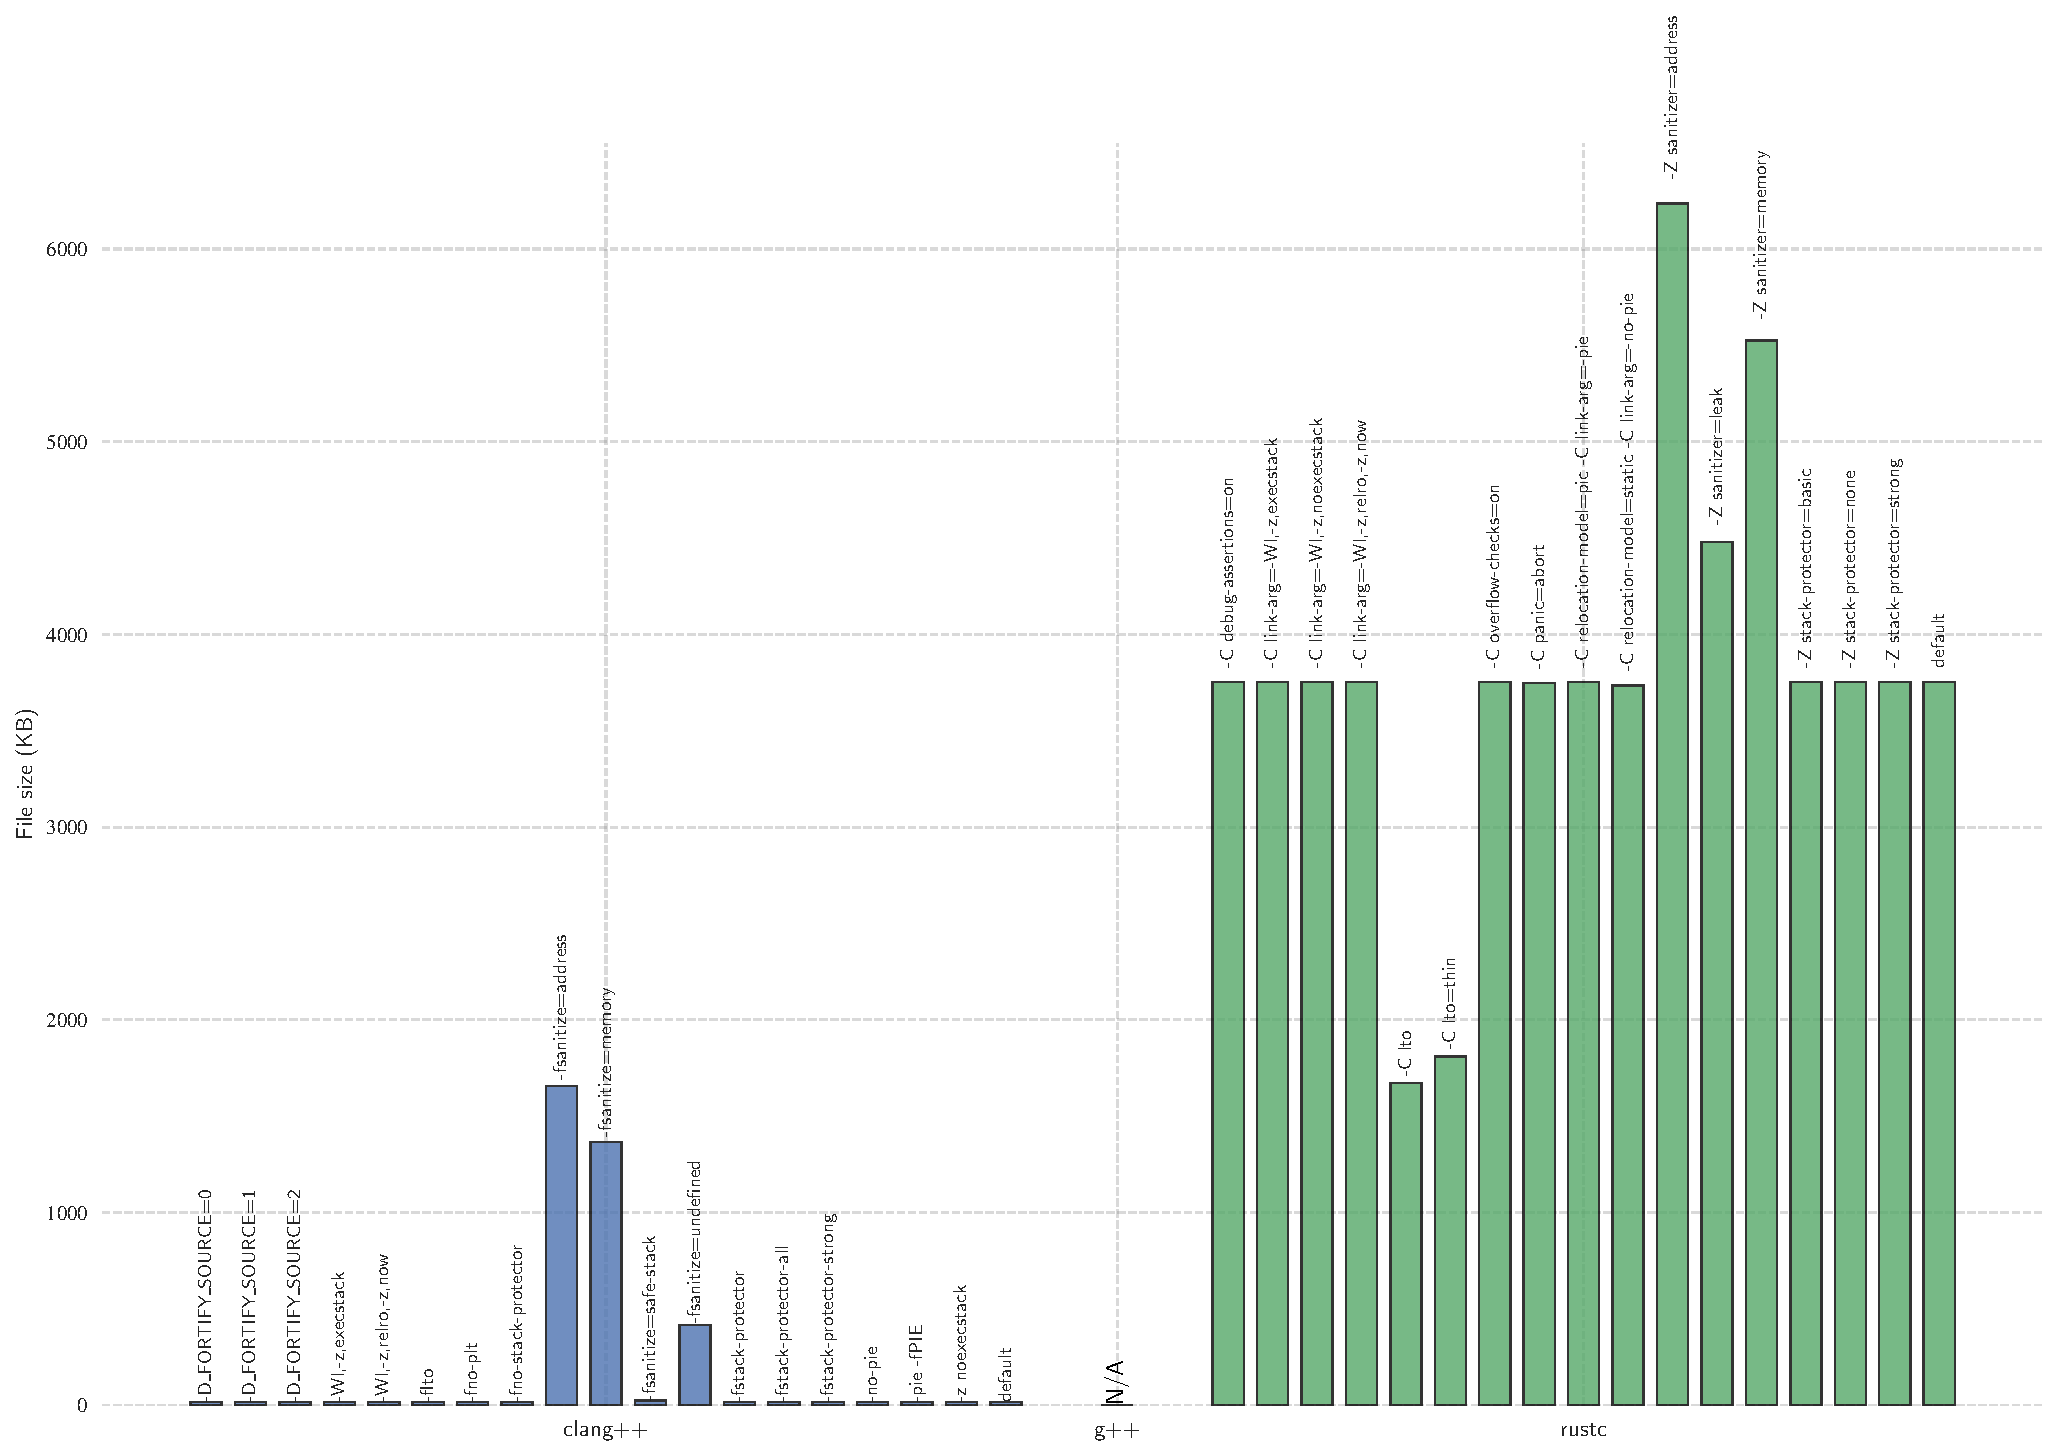
\includegraphics[width=\linewidth]{Gráficas/Gráficas_por_optimización/-Oz/File_size_KB.pdf}
      \label{fig:Gráficas_gráficas_por_optimización__oz_file_size_kb}
    }
  \end{minipage}
  \hfill
  \begin{minipage}{0.48\textwidth}
    \centering
    \subfloat[Funciones fortificadas (\%)]{
      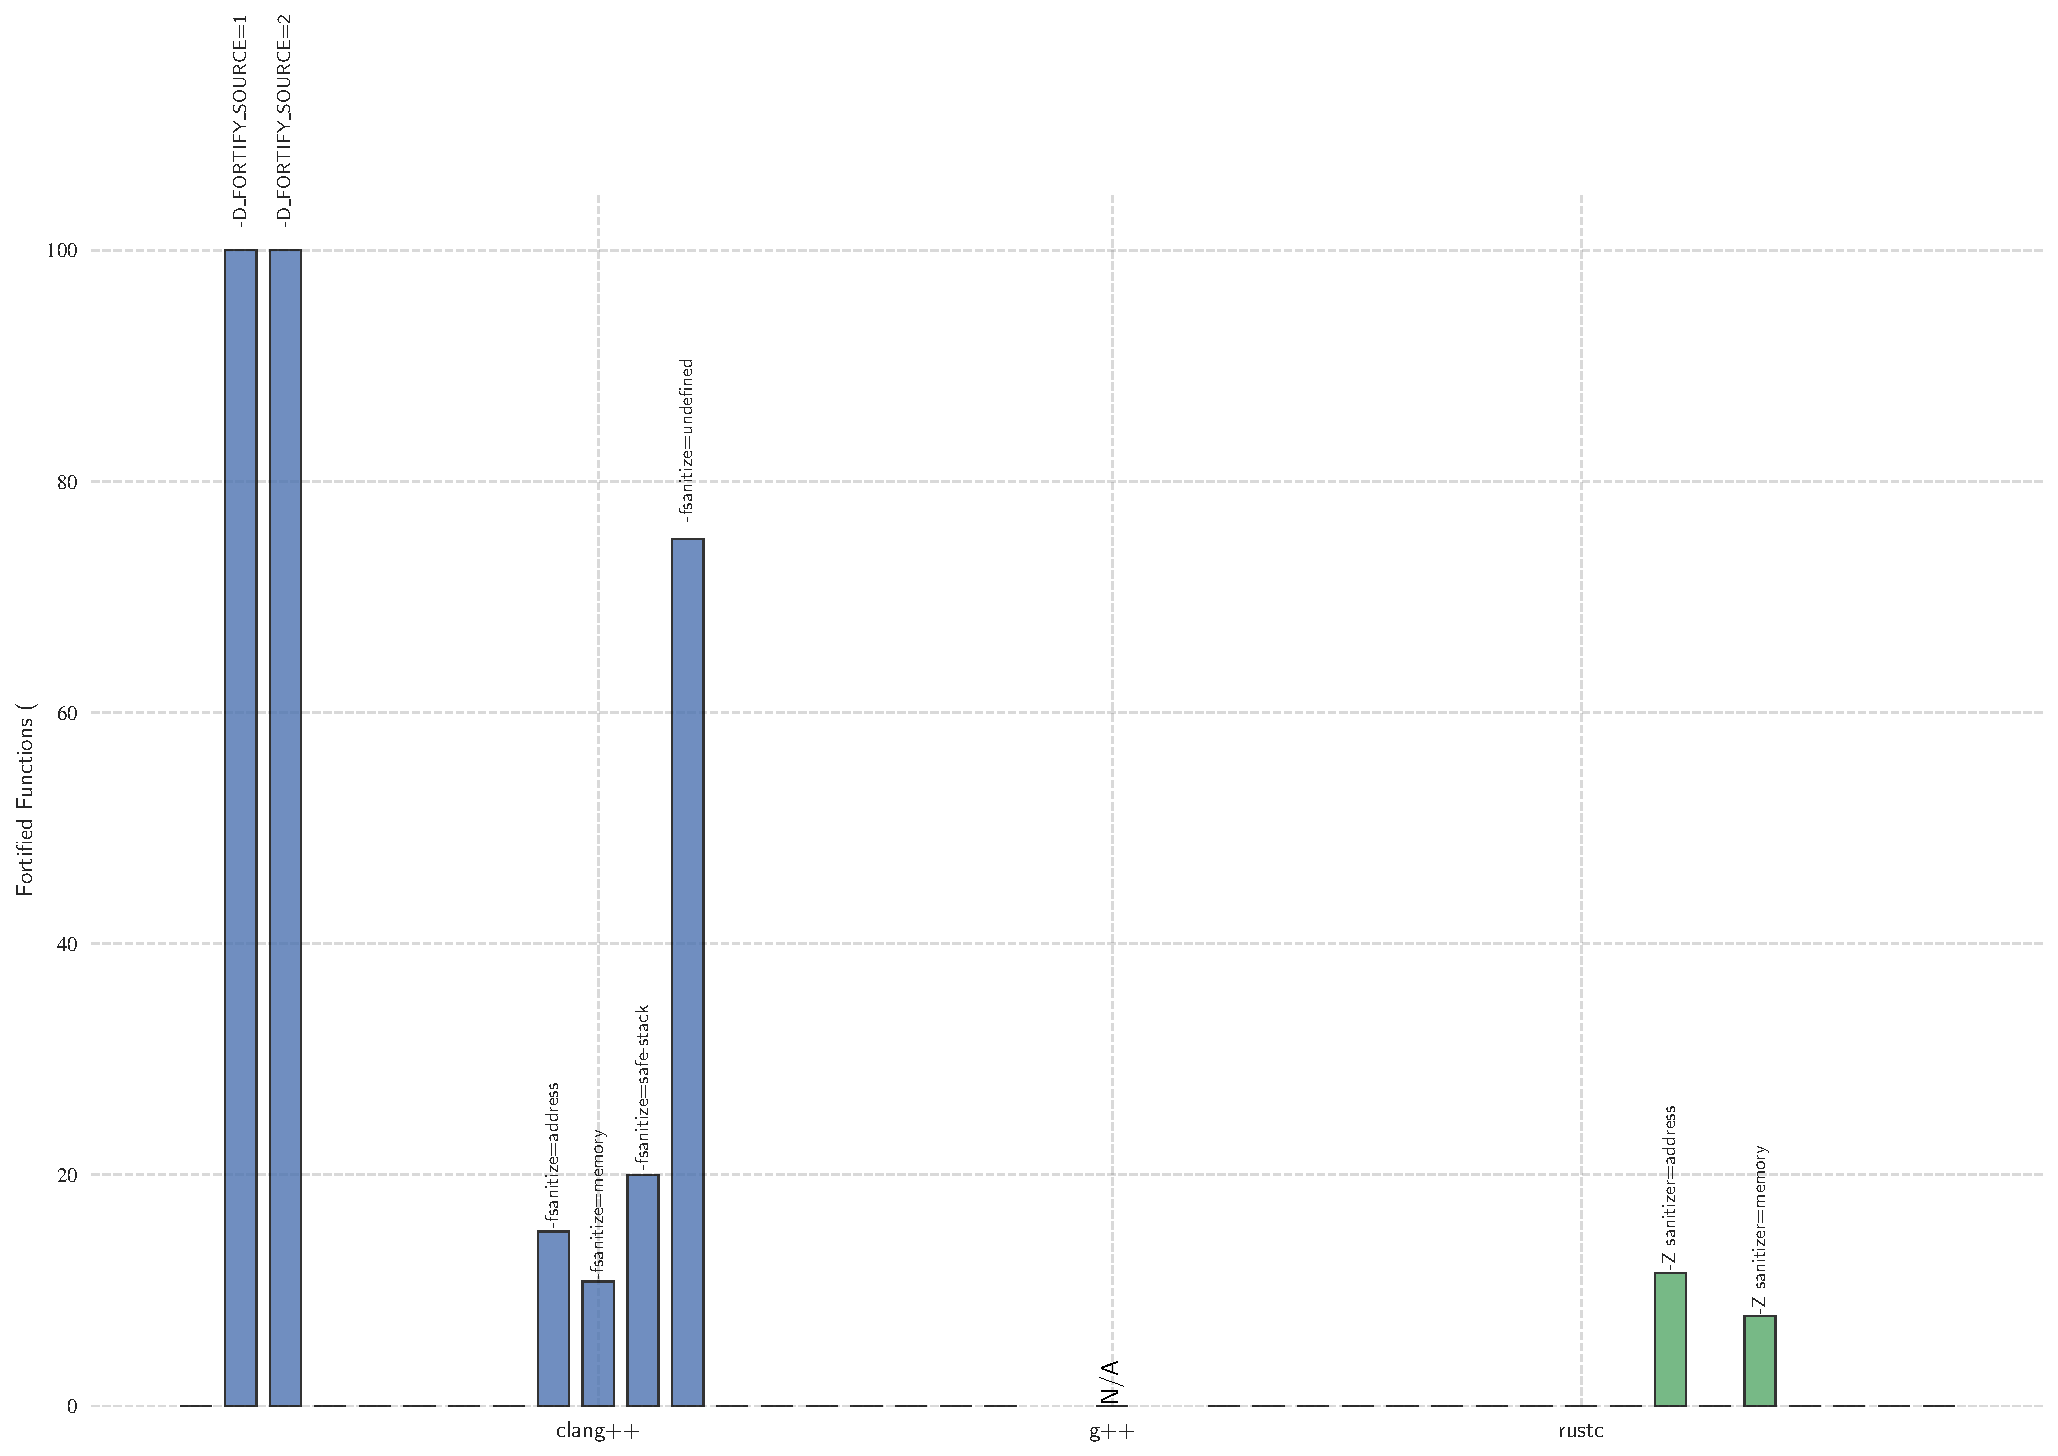
\includegraphics[width=\linewidth]{Gráficas/Gráficas_por_optimización/-Oz/Fortified_Functions.pdf}
      \label{fig:Gráficas_gráficas_por_optimización__oz_fortified_functions}
    }
  \end{minipage}


  \vspace{1cm}

  \begin{minipage}{0.48\textwidth}
    \centering
    \subfloat[Uso de memoria (KB)]{
      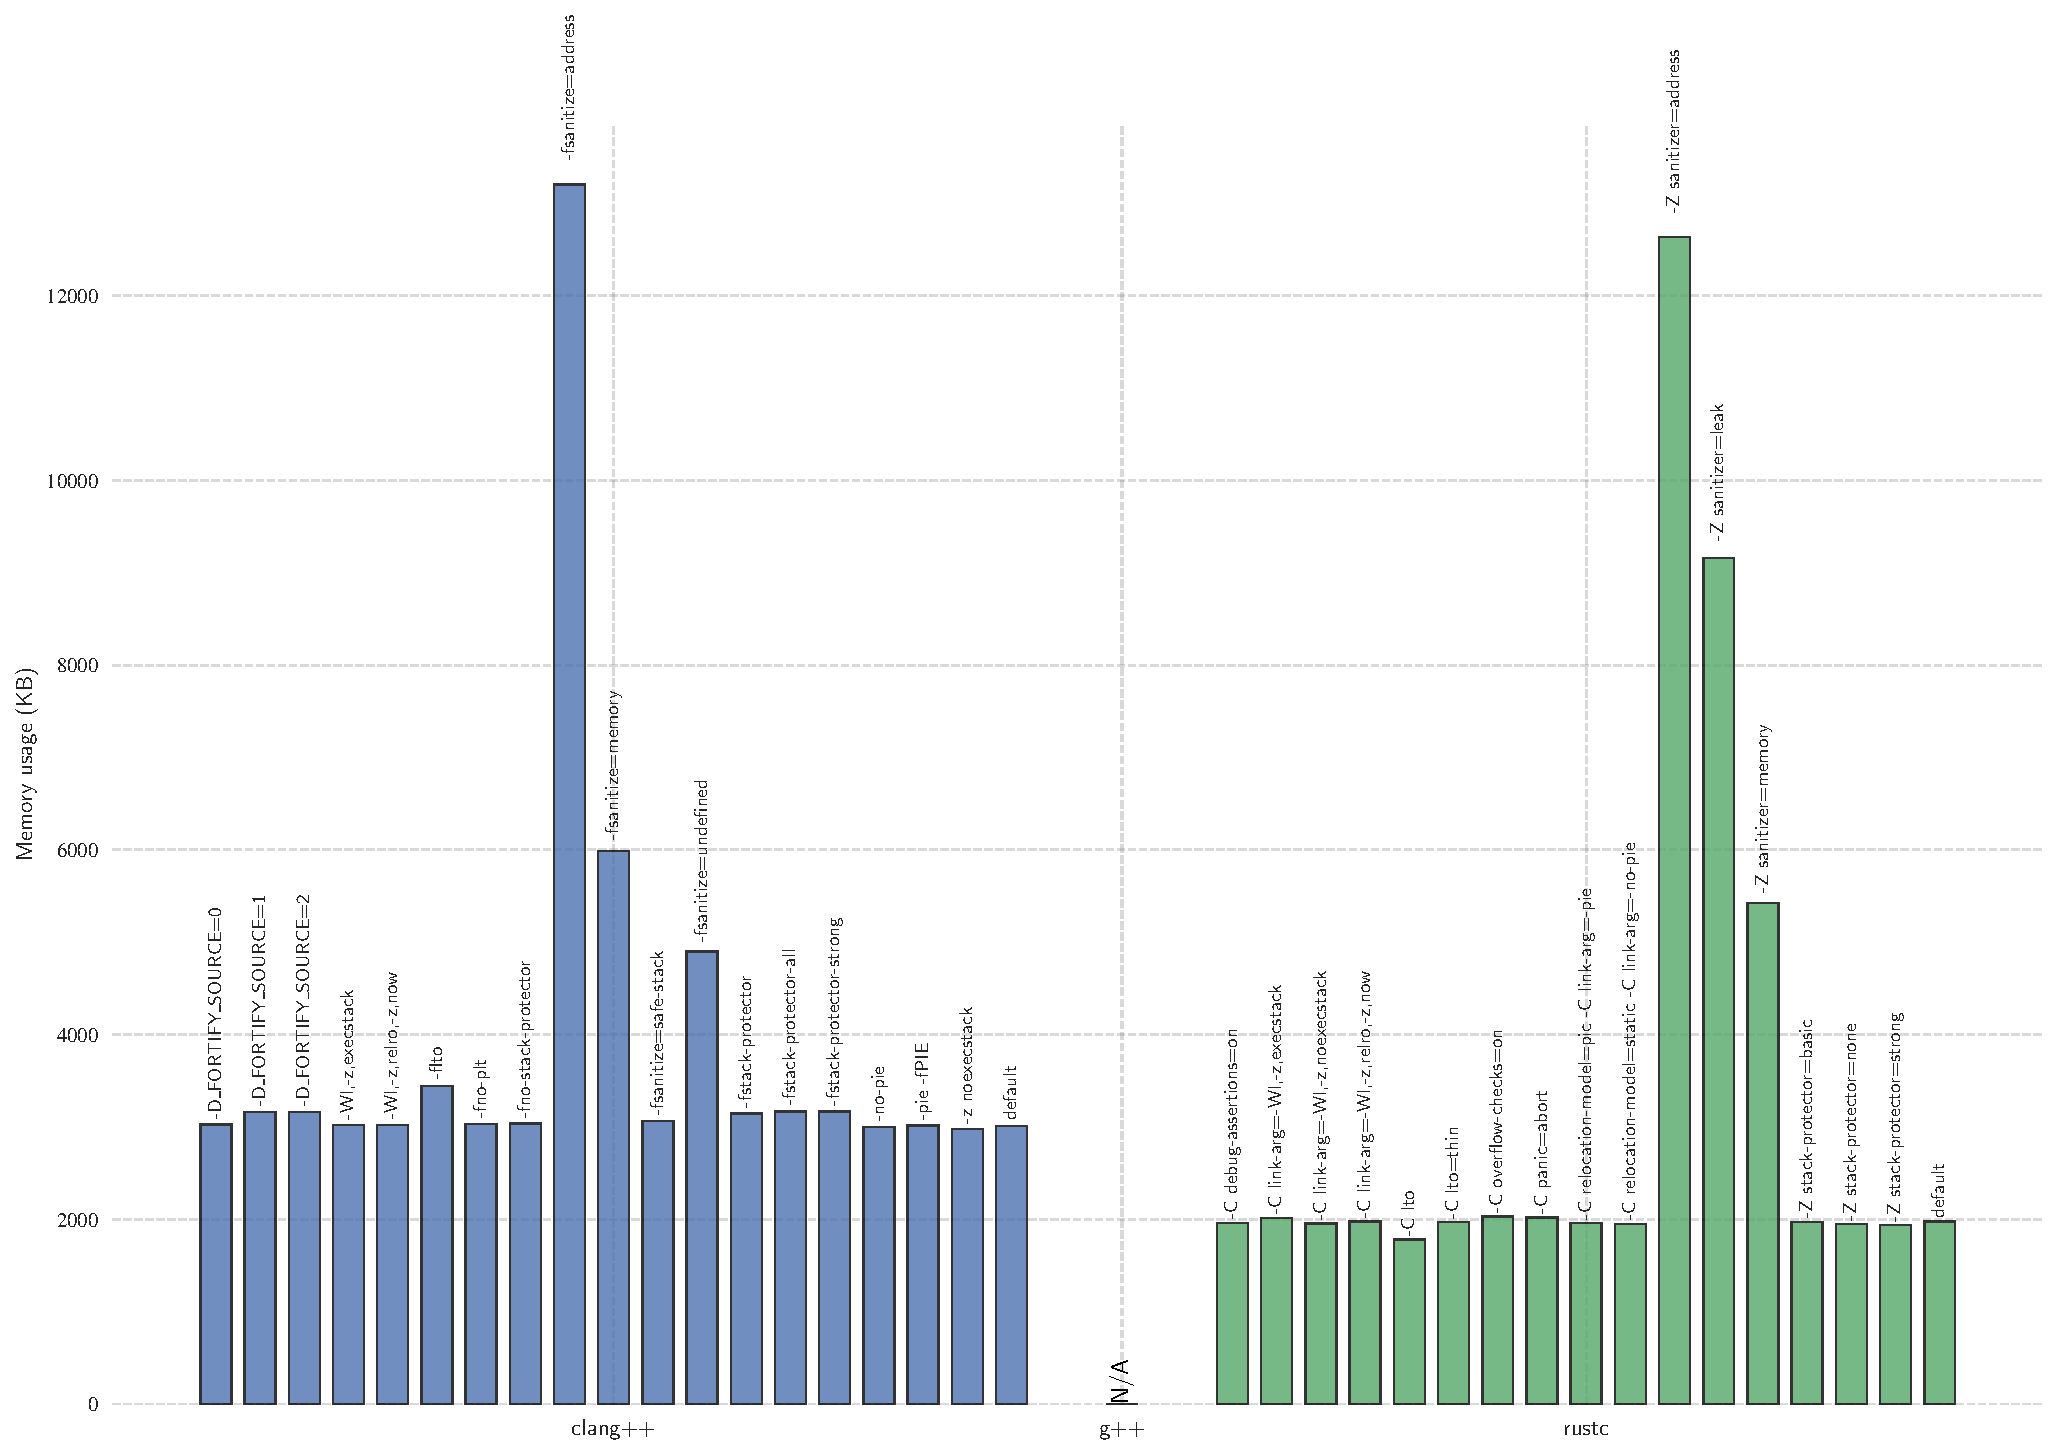
\includegraphics[width=\linewidth]{Gráficas/Gráficas_por_optimización/-Oz/Memory_usage_KB.pdf}
      \label{fig:Gráficas_gráficas_por_optimización__oz_memory_usage_kb}
    }
  \end{minipage}
  \hfill
  \begin{minipage}{0.48\textwidth}
    \centering
    \subfloat[Tiempo (ms)]{
      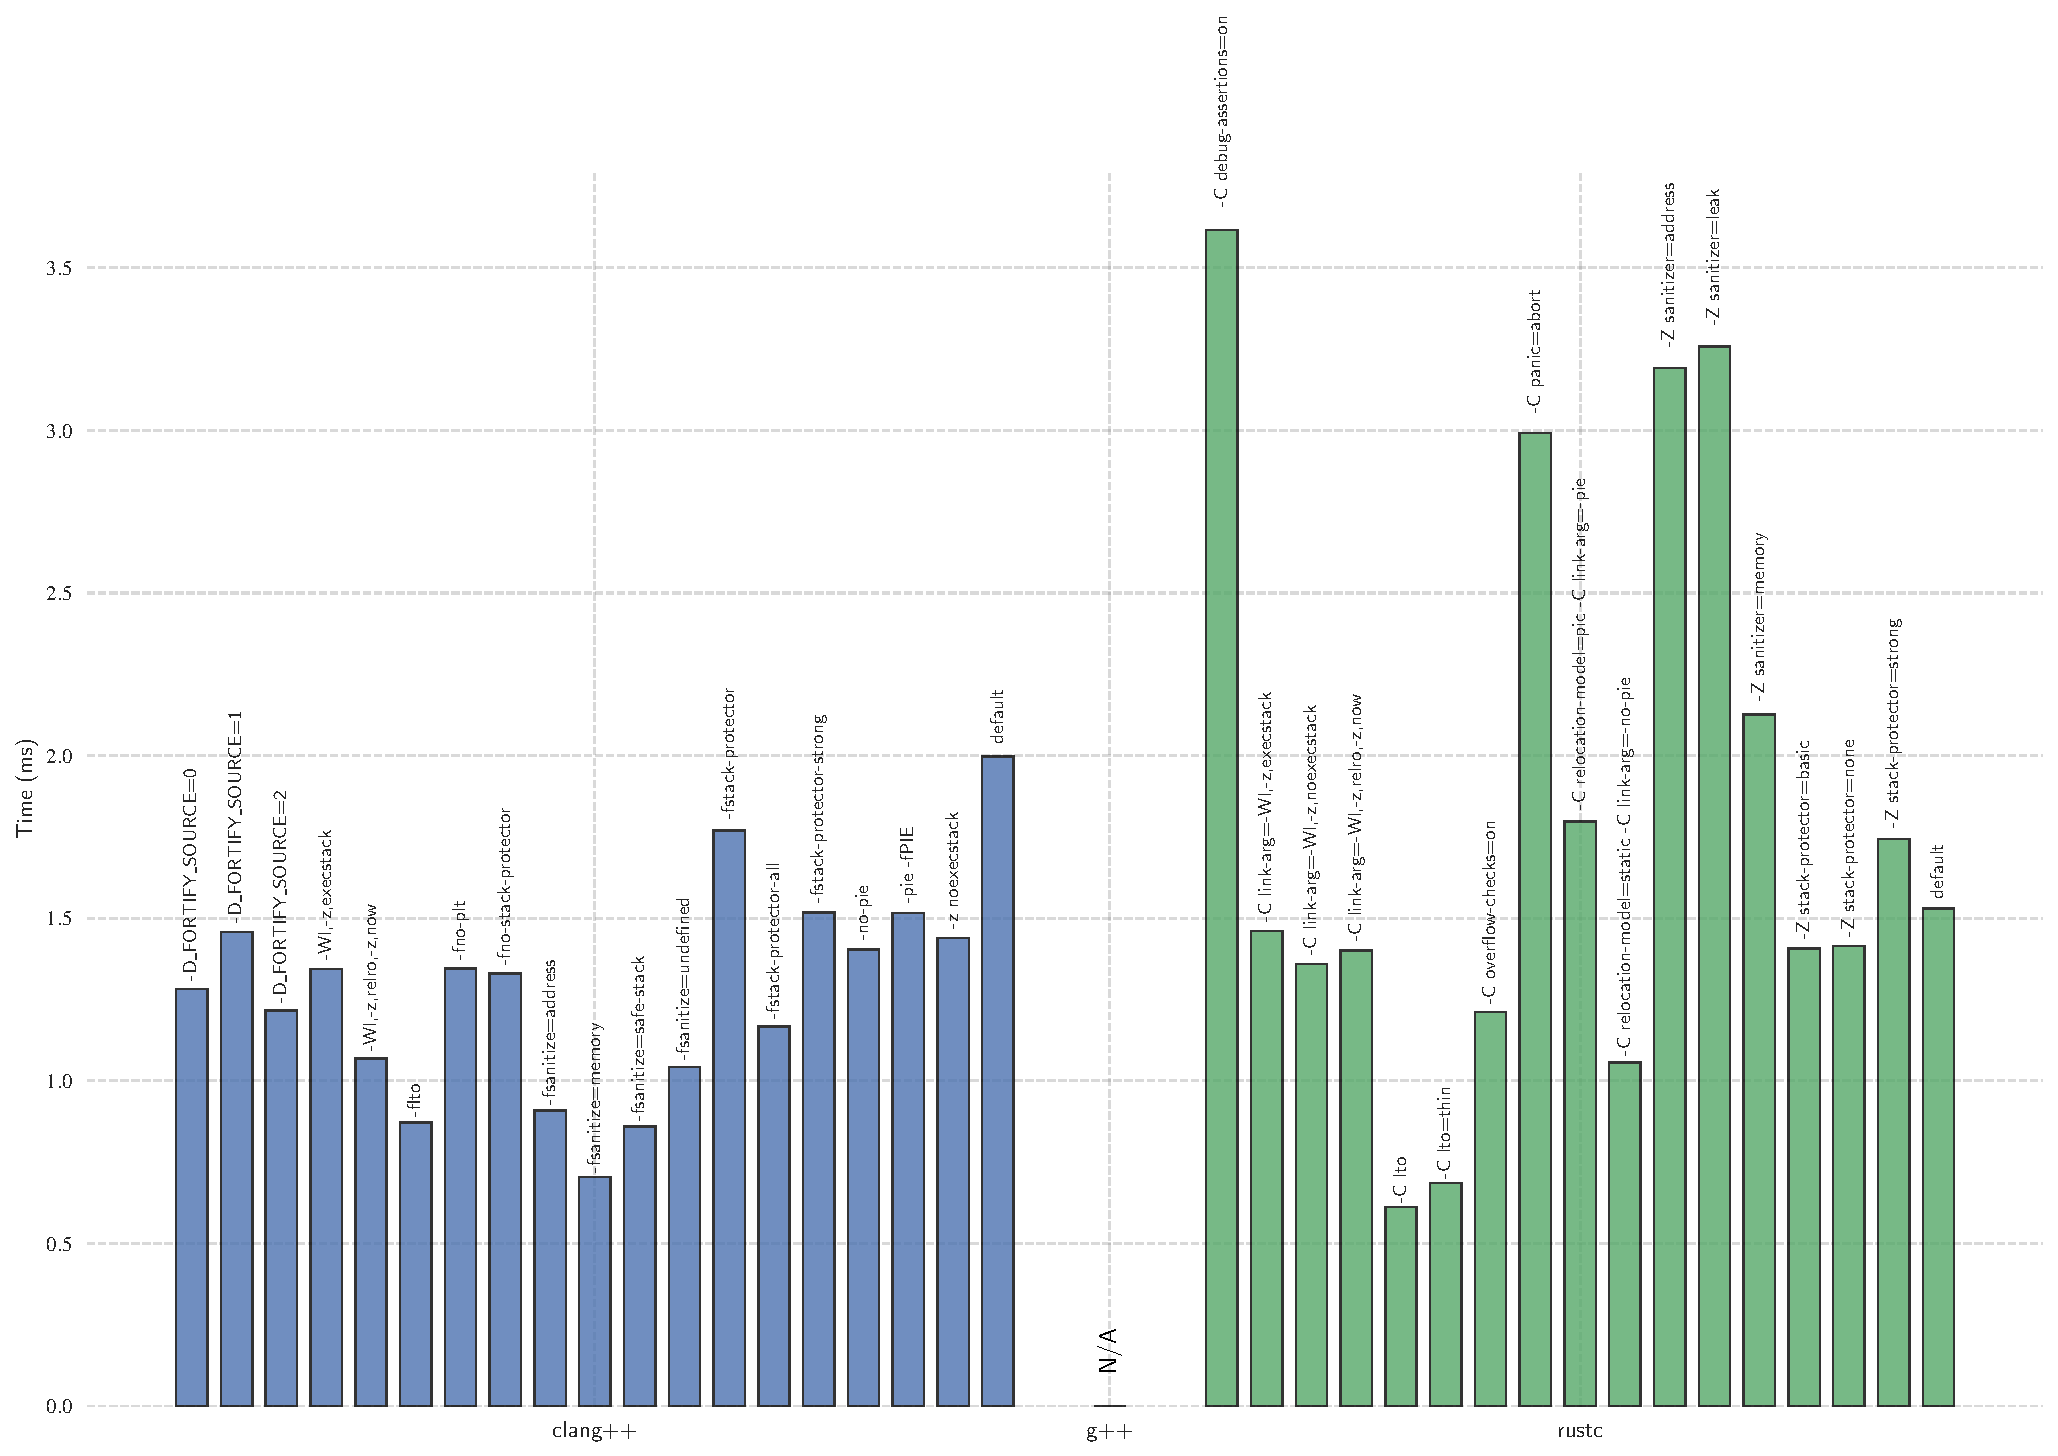
\includegraphics[width=\linewidth]{Gráficas/Gráficas_por_optimización/-Oz/Time_ms.pdf}
      \label{fig:Gráficas_gráficas_por_optimización__oz_time_ms}
    }
  \end{minipage}

\end{figure}
\newpage

\section*{Gráficas Por Medida Seguridad}

% === Gráficas_por_medida_seguridad/debug-assertions ===
\subsection*{Debug assertions}
\begin{figure}[htbp]
  \centering
  \caption{Resultados de compilación con optimización Debug assertions}
  \vspace{0.5cm}

  \begin{minipage}{0.48\textwidth}
    \centering
    \subfloat[Tamaño del archivo (KB)]{
      
\includegraphics[width=\linewidth]{Gráficas/Gráficas_por_medida_seguridad/debug-assertions/File_size_KB.pdf}
      \label{fig:Gráficas_gráficas_por_medida_seguridad_debug_assertions_file_size_kb}
    }
  \end{minipage}
  \hfill
  \begin{minipage}{0.48\textwidth}
    \centering
    \subfloat[Funciones fortificadas (\%)]{
      \includegraphics[width=\linewidth]{Gráficas/Gráficas_por_medida_seguridad/debug-assertions/Fortified_Functions.pdf}
      \label{fig:Gráficas_gráficas_por_medida_seguridad_debug_assertions_fortified_functions}
    }
  \end{minipage}


  \vspace{1cm}

  \begin{minipage}{0.48\textwidth}
    \centering
    \subfloat[Uso de memoria (KB)]{
      
\includegraphics[width=\linewidth]{Gráficas/Gráficas_por_medida_seguridad/debug-assertions/Memory_usage_KB.pdf}
      \label{fig:Gráficas_gráficas_por_medida_seguridad_debug_assertions_memory_usage_kb}
    }
  \end{minipage}
  \hfill
  \begin{minipage}{0.48\textwidth}
    \centering
    \subfloat[Tiempo (ms)]{
      
\includegraphics[width=\linewidth]{Gráficas/Gráficas_por_medida_seguridad/debug-assertions/Time_ms.pdf}
      \label{fig:Gráficas_gráficas_por_medida_seguridad_debug_assertions_time_ms}
    }
  \end{minipage}

\end{figure}
\newpage

% === Gráficas_por_medida_seguridad/execstack/disabled ===
\subsection*{Execstack / disabled}
\begin{figure}[htbp]
  \centering
  \caption{Resultados para Execstack (disabled)}
  \vspace{0.5cm}

  \begin{minipage}{0.48\textwidth}
    \centering
    \subfloat[Tamaño del archivo (KB)]{
      
\includegraphics[width=\linewidth]{Gráficas/Gráficas_por_medida_seguridad/execstack/disabled/File_size_KB.pdf}
      \label{fig:Gráficas_gráficas_por_medida_seguridad_execstack_disabled_file_size_kb}
    }
  \end{minipage}
  \hfill
  \begin{minipage}{0.48\textwidth}
    \centering
    \subfloat[Funciones fortificadas (\%)]{
      \includegraphics[width=\linewidth]{Gráficas/Gráficas_por_medida_seguridad/execstack/disabled/Fortified_Functions.pdf}
      \label{fig:Gráficas_gráficas_por_medida_seguridad_execstack_disabled_fortified_functions}
    }
  \end{minipage}


  \vspace{1cm}

  \begin{minipage}{0.48\textwidth}
    \centering
    \subfloat[Uso de memoria (KB)]{
      
\includegraphics[width=\linewidth]{Gráficas/Gráficas_por_medida_seguridad/execstack/disabled/Memory_usage_KB.pdf}
      \label{fig:Gráficas_gráficas_por_medida_seguridad_execstack_disabled_memory_usage_kb}
    }
  \end{minipage}
  \hfill
  \begin{minipage}{0.48\textwidth}
    \centering
    \subfloat[Tiempo (ms)]{
      
\includegraphics[width=\linewidth]{Gráficas/Gráficas_por_medida_seguridad/execstack/disabled/Time_ms.pdf}
      \label{fig:Gráficas_gráficas_por_medida_seguridad_execstack_disabled_time_ms}
    }
  \end{minipage}

\end{figure}
\newpage

% === Gráficas_por_medida_seguridad/execstack/enabled ===
\subsection*{Execstack / enabled}
\begin{figure}[htbp]
  \centering
  \caption{Resultados para Execstack (enabled)}
  \vspace{0.5cm}

  \begin{minipage}{0.48\textwidth}
    \centering
    \subfloat[Tamaño del archivo (KB)]{
      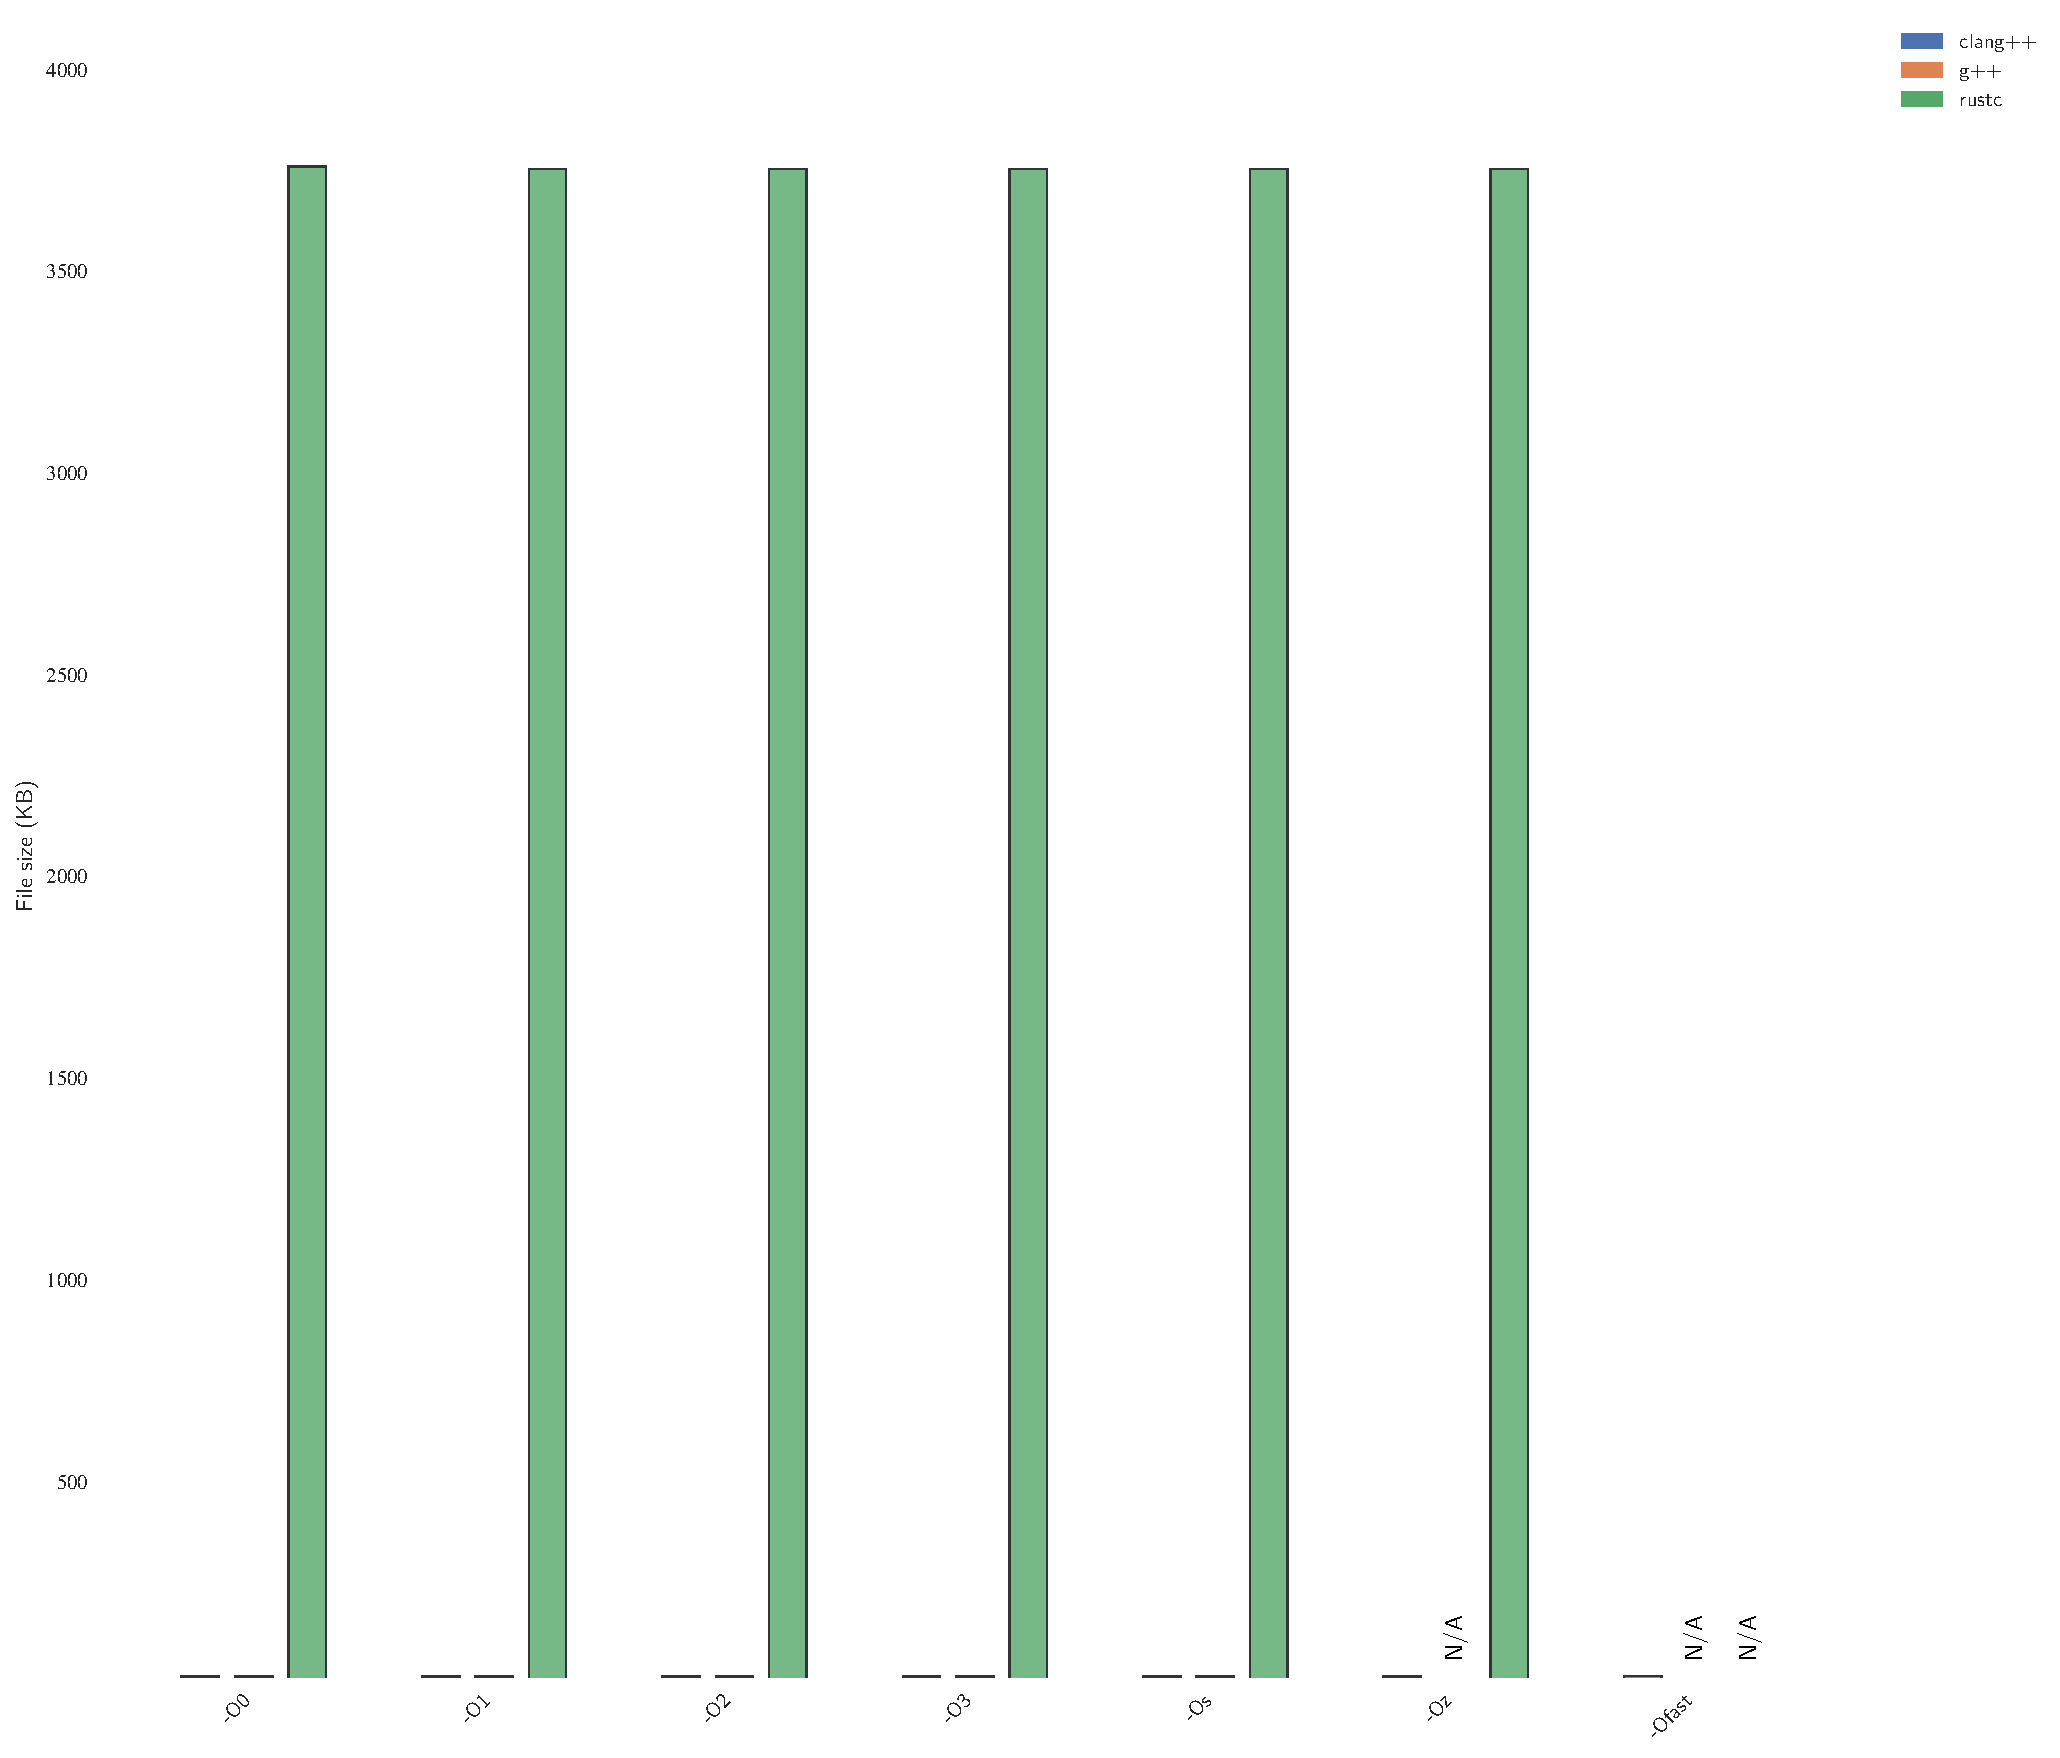
\includegraphics[width=\linewidth]{Gráficas/Gráficas_por_medida_seguridad/execstack/enabled/File_size_KB.pdf}
      \label{fig:Gráficas_gráficas_por_medida_seguridad_execstack_enabled_file_size_kb}
    }
  \end{minipage}
  \hfill
  \begin{minipage}{0.48\textwidth}
    \centering
    \subfloat[Funciones fortificadas (\%)]{
      \includegraphics[width=\linewidth]{Gráficas/Gráficas_por_medida_seguridad/execstack/enabled/Fortified_Functions.pdf}
      \label{fig:Gráficas_gráficas_por_medida_seguridad_execstack_enabled_fortified_functions}
    }
  \end{minipage}


  \vspace{1cm}

  \begin{minipage}{0.48\textwidth}
    \centering
    \subfloat[Uso de memoria (KB)]{
      
\includegraphics[width=\linewidth]{Gráficas/Gráficas_por_medida_seguridad/execstack/enabled/Memory_usage_KB.pdf}
      \label{fig:Gráficas_gráficas_por_medida_seguridad_execstack_enabled_memory_usage_kb}
    }
  \end{minipage}
  \hfill
  \begin{minipage}{0.48\textwidth}
    \centering
    \subfloat[Tiempo (ms)]{
      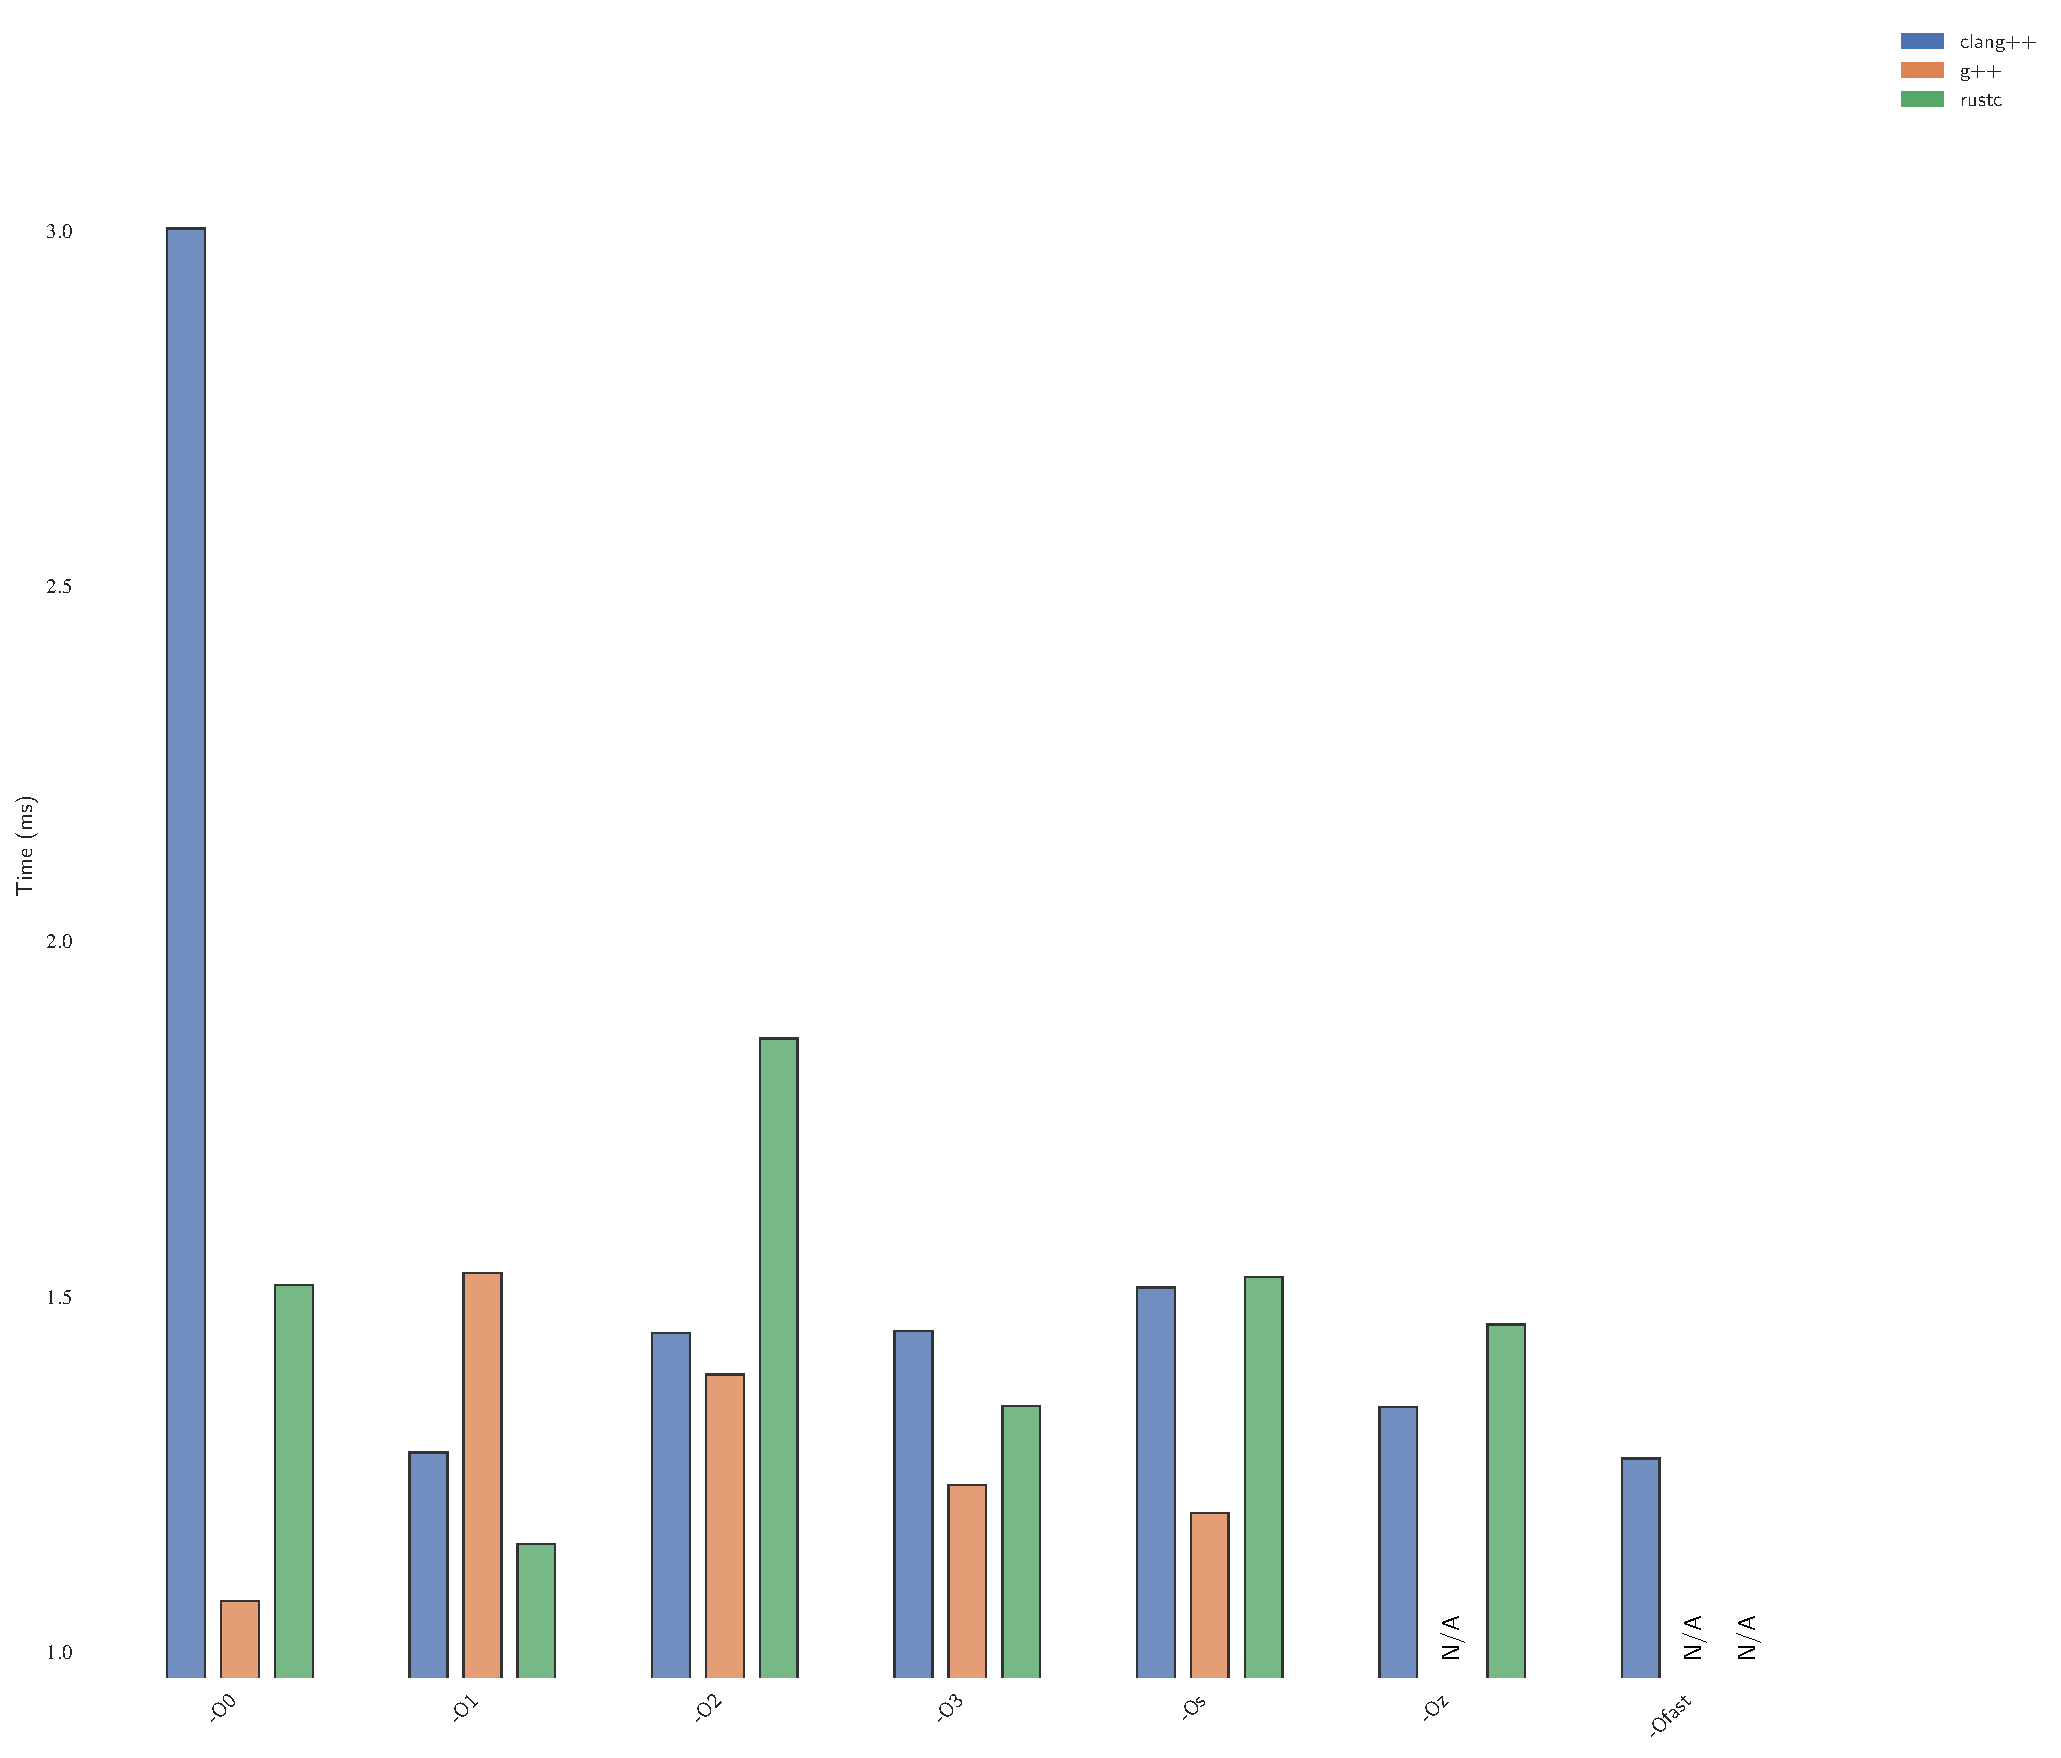
\includegraphics[width=\linewidth]{Gráficas/Gráficas_por_medida_seguridad/execstack/enabled/Time_ms.pdf}
      \label{fig:Gráficas_gráficas_por_medida_seguridad_execstack_enabled_time_ms}
    }
  \end{minipage}

\end{figure}
\newpage

% === Gráficas_por_medida_seguridad/fortify-source/disabled ===
\subsection*{Fortify source / disabled}
\begin{figure}[htbp]
  \centering
  \caption{Resultados para Fortify source (disabled)}
  \vspace{0.5cm}

  \begin{minipage}{0.48\textwidth}
    \centering
    \subfloat[Tamaño del archivo (KB)]{
      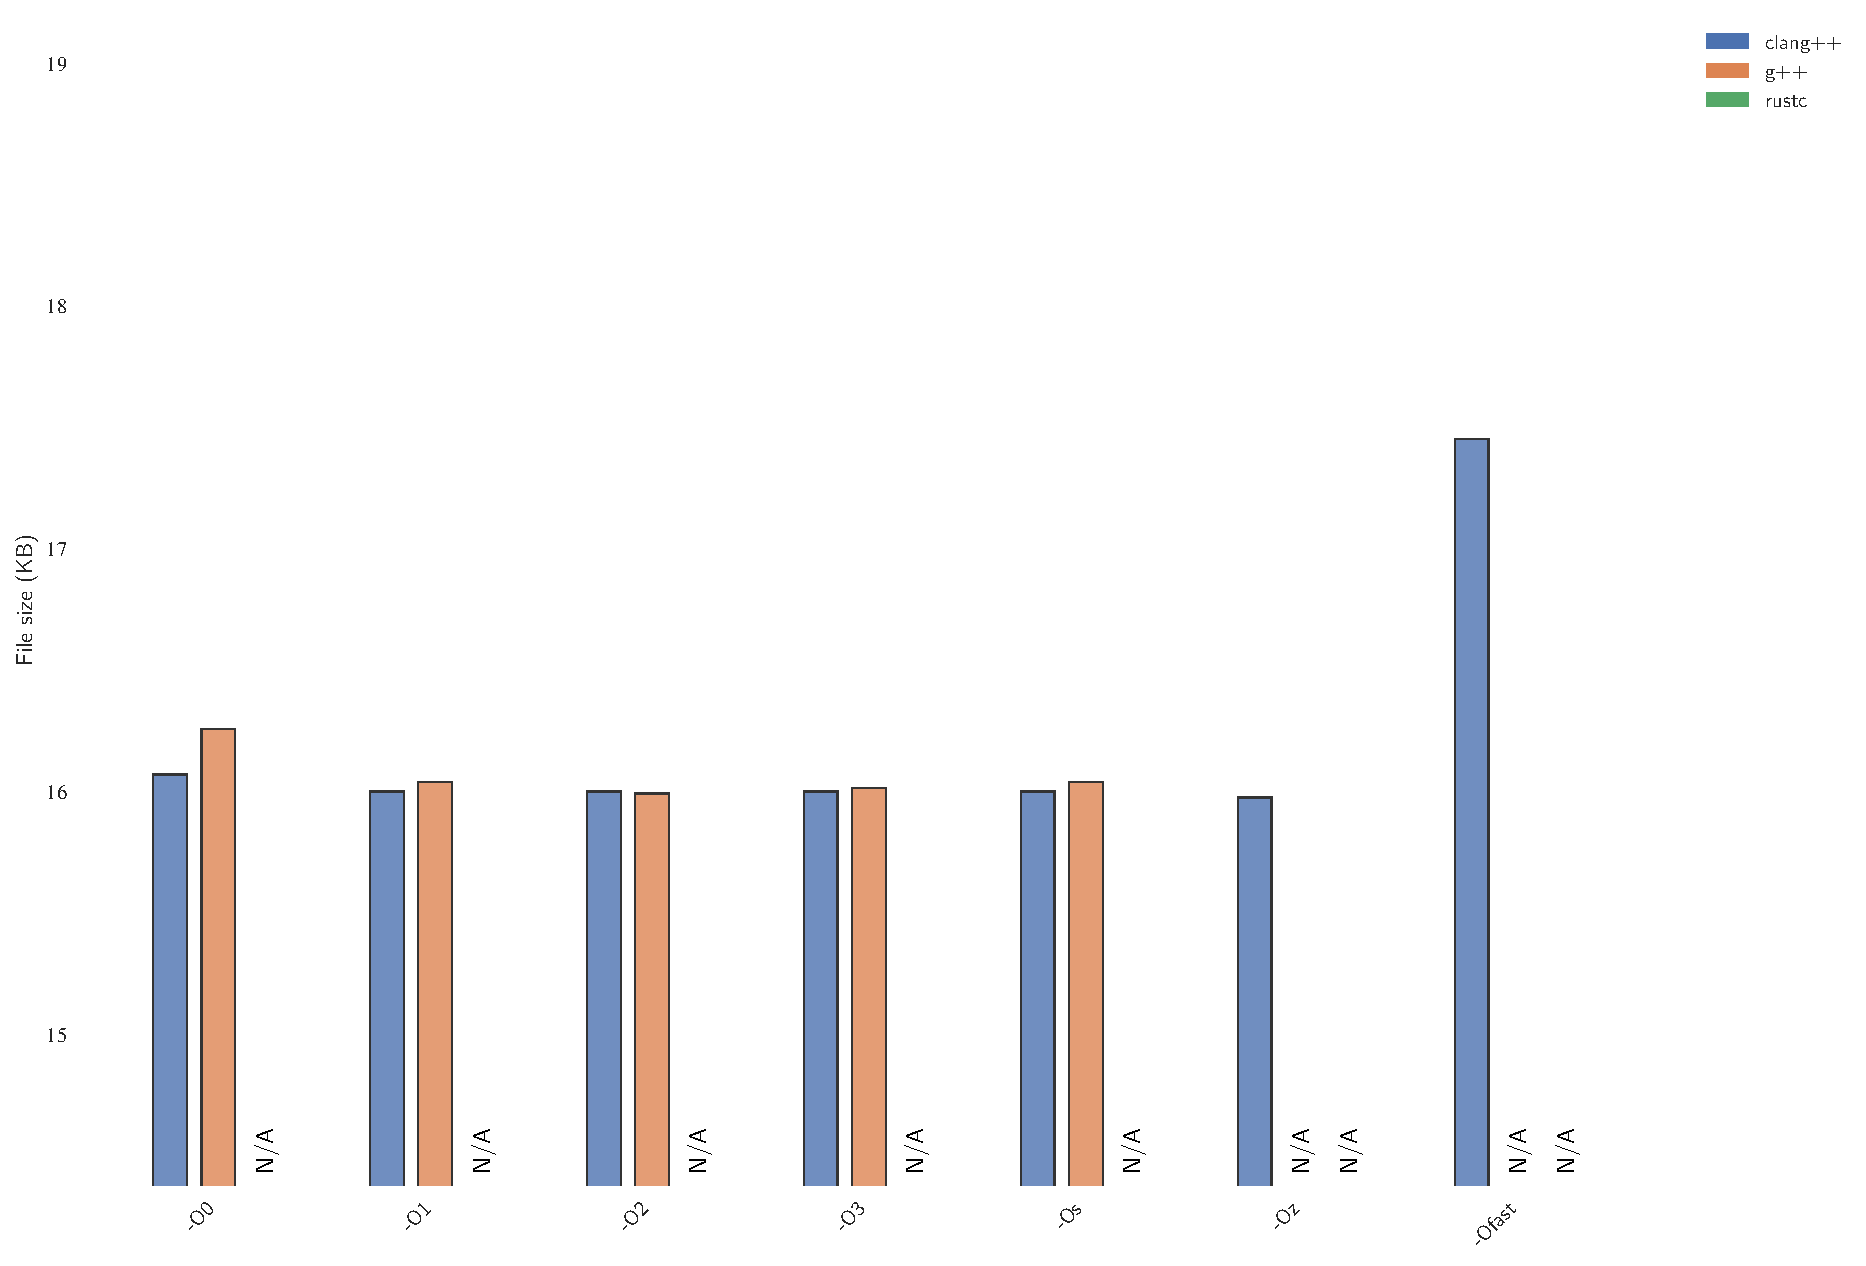
\includegraphics[width=\linewidth]{Gráficas/Gráficas_por_medida_seguridad/fortify-source/disabled/File_size_KB.pdf}
      \label{fig:Gráficas_gráficas_por_medida_seguridad_fortify_source_disabled_file_size_kb}
    }
  \end{minipage}
  \hfill
  \begin{minipage}{0.48\textwidth}
    \centering
    \subfloat[Funciones fortificadas (\%)]{
      \includegraphics[width=\linewidth]{Gráficas/Gráficas_por_medida_seguridad/fortify-source/disabled/Fortified_Functions.pdf}
      \label{fig:Gráficas_gráficas_por_medida_seguridad_fortify_source_disabled_fortified_functions}
    }
  \end{minipage}


  \vspace{1cm}

  \begin{minipage}{0.48\textwidth}
    \centering
    \subfloat[Uso de memoria (KB)]{
      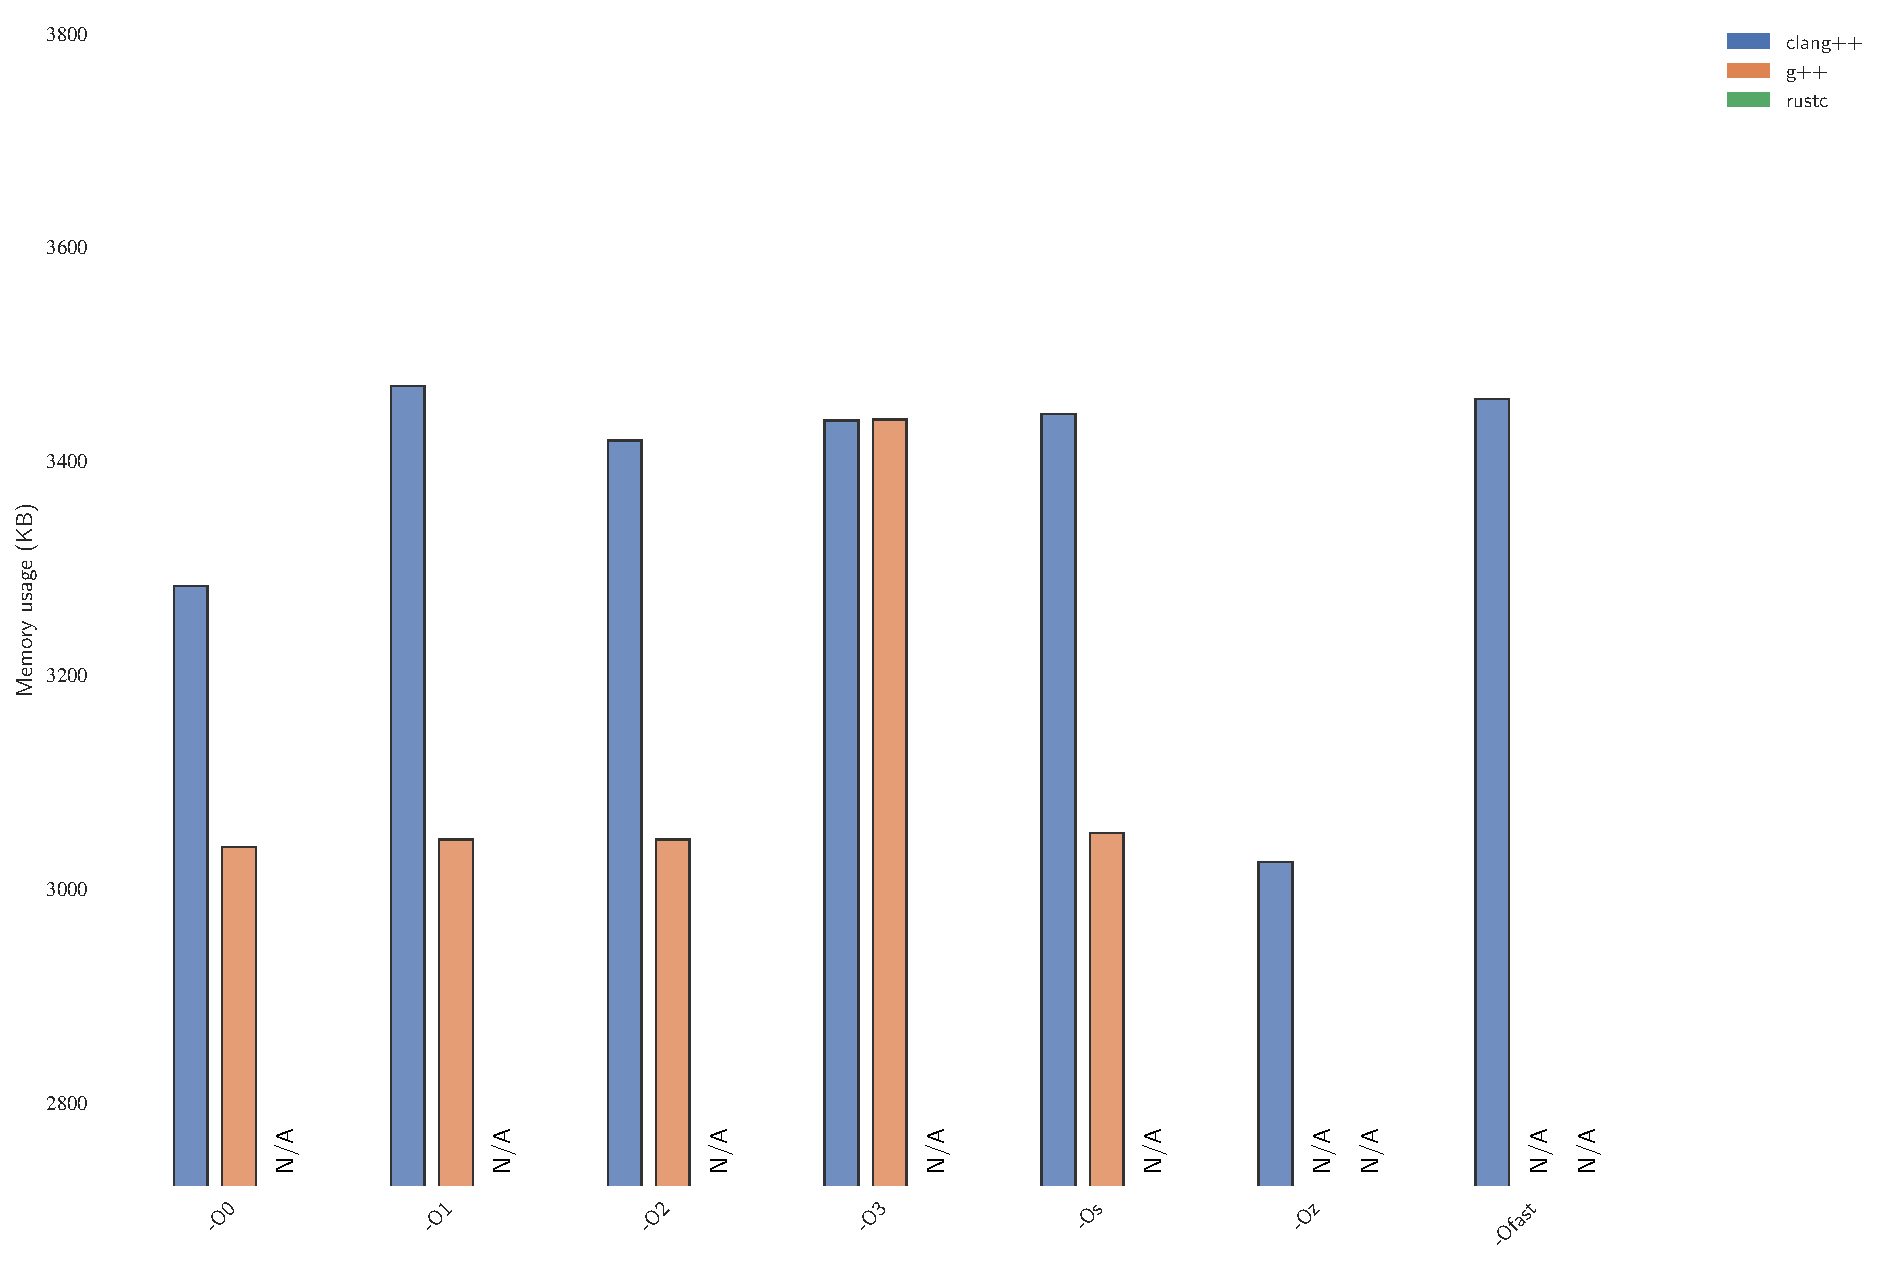
\includegraphics[width=\linewidth]{Gráficas/Gráficas_por_medida_seguridad/fortify-source/disabled/Memory_usage_KB.pdf}
      \label{fig:Gráficas_gráficas_por_medida_seguridad_fortify_source_disabled_memory_usage_kb}
    }
  \end{minipage}
  \hfill
  \begin{minipage}{0.48\textwidth}
    \centering
    \subfloat[Tiempo (ms)]{
      
\includegraphics[width=\linewidth]{Gráficas/Gráficas_por_medida_seguridad/fortify-source/disabled/Time_ms.pdf}
      \label{fig:Gráficas_gráficas_por_medida_seguridad_fortify_source_disabled_time_ms}
    }
  \end{minipage}

\end{figure}
\newpage

% === Gráficas_por_medida_seguridad/fortify-source/level-1 ===
\subsection*{Fortify source / level-1}
\begin{figure}[htbp]
  \centering
  \caption{Resultados para Fortify source (level-1)}
  \vspace{0.5cm}

  \begin{minipage}{0.48\textwidth}
    \centering
    \subfloat[Tamaño del archivo (KB)]{
      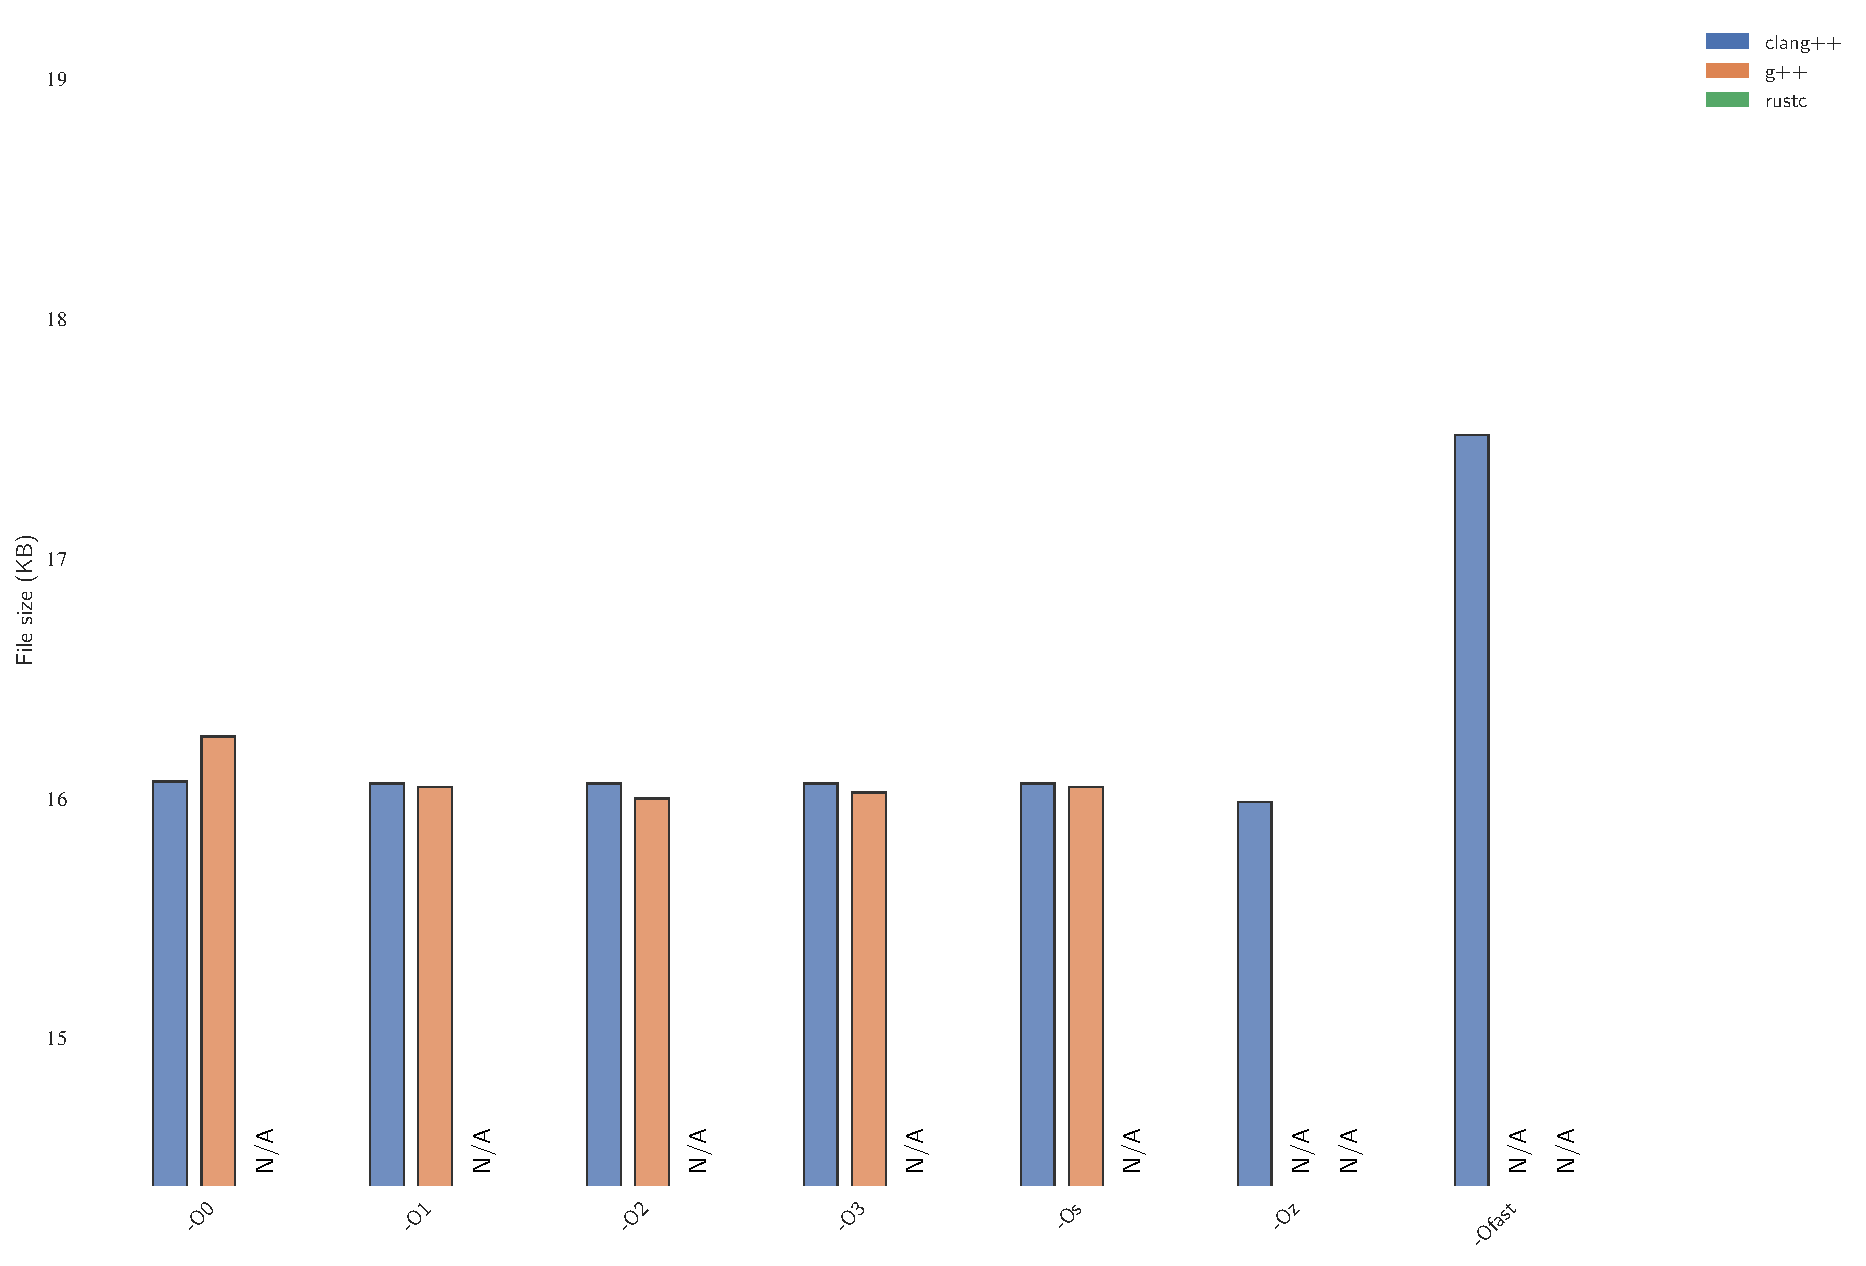
\includegraphics[width=\linewidth]{Gráficas/Gráficas_por_medida_seguridad/fortify-source/level-1/File_size_KB.pdf}
      \label{fig:Gráficas_gráficas_por_medida_seguridad_fortify_source_level_1_file_size_kb}
    }
  \end{minipage}
  \hfill
  \begin{minipage}{0.48\textwidth}
    \centering
    \subfloat[Funciones fortificadas (\%)]{
      \includegraphics[width=\linewidth]{Gráficas/Gráficas_por_medida_seguridad/fortify-source/level-1/Fortified_Functions.pdf}
      \label{fig:Gráficas_gráficas_por_medida_seguridad_fortify_source_level_1_fortified_functions}
    }
  \end{minipage}


  \vspace{1cm}

  \begin{minipage}{0.48\textwidth}
    \centering
    \subfloat[Uso de memoria (KB)]{
      
\includegraphics[width=\linewidth]{Gráficas/Gráficas_por_medida_seguridad/fortify-source/level-1/Memory_usage_KB.pdf}
      \label{fig:Gráficas_gráficas_por_medida_seguridad_fortify_source_level_1_memory_usage_kb}
    }
  \end{minipage}
  \hfill
  \begin{minipage}{0.48\textwidth}
    \centering
    \subfloat[Tiempo (ms)]{
      
\includegraphics[width=\linewidth]{Gráficas/Gráficas_por_medida_seguridad/fortify-source/level-1/Time_ms.pdf}
      \label{fig:Gráficas_gráficas_por_medida_seguridad_fortify_source_level_1_time_ms}
    }
  \end{minipage}

\end{figure}
\newpage

% === Gráficas_por_medida_seguridad/fortify-source/level-2 ===
\subsection*{Fortify source / level-2}
\begin{figure}[htbp]
  \centering
  \caption{Resultados para Fortify source (level-2)}
  \vspace{0.5cm}

  \begin{minipage}{0.48\textwidth}
    \centering
    \subfloat[Tamaño del archivo (KB)]{
      
\includegraphics[width=\linewidth]{Gráficas/Gráficas_por_medida_seguridad/fortify-source/level-2/File_size_KB.pdf}
      \label{fig:Gráficas_gráficas_por_medida_seguridad_fortify_source_level_2_file_size_kb}
    }
  \end{minipage}
  \hfill
  \begin{minipage}{0.48\textwidth}
    \centering
    \subfloat[Funciones fortificadas (\%)]{
      \includegraphics[width=\linewidth]{Gráficas/Gráficas_por_medida_seguridad/fortify-source/level-2/Fortified_Functions.pdf}
      \label{fig:Gráficas_gráficas_por_medida_seguridad_fortify_source_level_2_fortified_functions}
    }
  \end{minipage}


  \vspace{1cm}

  \begin{minipage}{0.48\textwidth}
    \centering
    \subfloat[Uso de memoria (KB)]{
      
\includegraphics[width=\linewidth]{Gráficas/Gráficas_por_medida_seguridad/fortify-source/level-2/Memory_usage_KB.pdf}
      \label{fig:Gráficas_gráficas_por_medida_seguridad_fortify_source_level_2_memory_usage_kb}
    }
  \end{minipage}
  \hfill
  \begin{minipage}{0.48\textwidth}
    \centering
    \subfloat[Tiempo (ms)]{
      
\includegraphics[width=\linewidth]{Gráficas/Gráficas_por_medida_seguridad/fortify-source/level-2/Time_ms.pdf}
      \label{fig:Gráficas_gráficas_por_medida_seguridad_fortify_source_level_2_time_ms}
    }
  \end{minipage}

\end{figure}
\newpage

% === Gráficas_por_medida_seguridad/overflow-checks ===
\subsection*{Overflow checks}
\begin{figure}[htbp]
  \centering
  \caption{Resultados de compilación con optimización Overflow checks}
  \vspace{0.5cm}

  \begin{minipage}{0.48\textwidth}
    \centering
    \subfloat[Tamaño del archivo (KB)]{
      
\includegraphics[width=\linewidth]{Gráficas/Gráficas_por_medida_seguridad/overflow-checks/File_size_KB.pdf}
      \label{fig:Gráficas_gráficas_por_medida_seguridad_overflow_checks_file_size_kb}
    }
  \end{minipage}
  \hfill
  \begin{minipage}{0.48\textwidth}
    \centering
    \subfloat[Funciones fortificadas (\%)]{
      \includegraphics[width=\linewidth]{Gráficas/Gráficas_por_medida_seguridad/overflow-checks/Fortified_Functions.pdf}
      \label{fig:Gráficas_gráficas_por_medida_seguridad_overflow_checks_fortified_functions}
    }
  \end{minipage}


  \vspace{1cm}

  \begin{minipage}{0.48\textwidth}
    \centering
    \subfloat[Uso de memoria (KB)]{
      
\includegraphics[width=\linewidth]{Gráficas/Gráficas_por_medida_seguridad/overflow-checks/Memory_usage_KB.pdf}
      \label{fig:Gráficas_gráficas_por_medida_seguridad_overflow_checks_memory_usage_kb}
    }
  \end{minipage}
  \hfill
  \begin{minipage}{0.48\textwidth}
    \centering
    \subfloat[Tiempo (ms)]{
      
\includegraphics[width=\linewidth]{Gráficas/Gráficas_por_medida_seguridad/overflow-checks/Time_ms.pdf}
      \label{fig:Gráficas_gráficas_por_medida_seguridad_overflow_checks_time_ms}
    }
  \end{minipage}

\end{figure}
\newpage

% === Gráficas_por_medida_seguridad/panic ===
\subsection*{panic}
\begin{figure}[htbp]
  \centering
  \caption{Resultados de compilación con optimización panic}
  \vspace{0.5cm}

  \begin{minipage}{0.48\textwidth}
    \centering
    \subfloat[Tamaño del archivo (KB)]{
      
\includegraphics[width=\linewidth]{Gráficas/Gráficas_por_medida_seguridad/panic/File_size_KB.pdf}
      \label{fig:Gráficas_gráficas_por_medida_seguridad_panic_file_size_kb}
    }
  \end{minipage}
  \hfill
  \begin{minipage}{0.48\textwidth}
    \centering
    \subfloat[Funciones fortificadas (\%)]{
      \includegraphics[width=\linewidth]{Gráficas/Gráficas_por_medida_seguridad/panic/Fortified_Functions.pdf}
      \label{fig:Gráficas_gráficas_por_medida_seguridad_panic_fortified_functions}
    }
  \end{minipage}


  \vspace{1cm}

  \begin{minipage}{0.48\textwidth}
    \centering
    \subfloat[Uso de memoria (KB)]{
      
\includegraphics[width=\linewidth]{Gráficas/Gráficas_por_medida_seguridad/panic/Memory_usage_KB.pdf}
      \label{fig:Gráficas_gráficas_por_medida_seguridad_panic_memory_usage_kb}
    }
  \end{minipage}
  \hfill
  \begin{minipage}{0.48\textwidth}
    \centering
    \subfloat[Tiempo (ms)]{
      
\includegraphics[width=\linewidth]{Gráficas/Gráficas_por_medida_seguridad/panic/Time_ms.pdf}
      \label{fig:Gráficas_gráficas_por_medida_seguridad_panic_time_ms}
    }
  \end{minipage}

\end{figure}
\newpage

% === Gráficas_por_medida_seguridad/pie/disabled ===
\subsection*{PIE / disabled}
\begin{figure}[htbp]
  \centering
  \caption{Resultados para PIE (disabled)}
  \vspace{0.5cm}

  \begin{minipage}{0.48\textwidth}
    \centering
    \subfloat[Tamaño del archivo (KB)]{
      
\includegraphics[width=\linewidth]{Gráficas/Gráficas_por_medida_seguridad/pie/disabled/File_size_KB.pdf}
      \label{fig:Gráficas_gráficas_por_medida_seguridad_pie_disabled_file_size_kb}
    }
  \end{minipage}
  \hfill
  \begin{minipage}{0.48\textwidth}
    \centering
    \subfloat[Funciones fortificadas (\%)]{
      \includegraphics[width=\linewidth]{Gráficas/Gráficas_por_medida_seguridad/pie/disabled/Fortified_Functions.pdf}
      \label{fig:Gráficas_gráficas_por_medida_seguridad_pie_disabled_fortified_functions}
    }
  \end{minipage}


  \vspace{1cm}

  \begin{minipage}{0.48\textwidth}
    \centering
    \subfloat[Uso de memoria (KB)]{
      
\includegraphics[width=\linewidth]{Gráficas/Gráficas_por_medida_seguridad/pie/disabled/Memory_usage_KB.pdf}
      \label{fig:Gráficas_gráficas_por_medida_seguridad_pie_disabled_memory_usage_kb}
    }
  \end{minipage}
  \hfill
  \begin{minipage}{0.48\textwidth}
    \centering
    \subfloat[Tiempo (ms)]{
      
\includegraphics[width=\linewidth]{Gráficas/Gráficas_por_medida_seguridad/pie/disabled/Time_ms.pdf}
      \label{fig:Gráficas_gráficas_por_medida_seguridad_pie_disabled_time_ms}
    }
  \end{minipage}

\end{figure}
\newpage

% === Gráficas_por_medida_seguridad/pie/enabled ===
\subsection*{PIE / enabled}
\begin{figure}[htbp]
  \centering
  \caption{Resultados para PIE (enabled)}
  \vspace{0.5cm}

  \begin{minipage}{0.48\textwidth}
    \centering
    \subfloat[Tamaño del archivo (KB)]{
      
\includegraphics[width=\linewidth]{Gráficas/Gráficas_por_medida_seguridad/pie/enabled/File_size_KB.pdf}
      \label{fig:Gráficas_gráficas_por_medida_seguridad_pie_enabled_file_size_kb}
    }
  \end{minipage}
  \hfill
  \begin{minipage}{0.48\textwidth}
    \centering
    \subfloat[Funciones fortificadas (\%)]{
      \includegraphics[width=\linewidth]{Gráficas/Gráficas_por_medida_seguridad/pie/enabled/Fortified_Functions.pdf}
      \label{fig:Gráficas_gráficas_por_medida_seguridad_pie_enabled_fortified_functions}
    }
  \end{minipage}


  \vspace{1cm}

  \begin{minipage}{0.48\textwidth}
    \centering
    \subfloat[Uso de memoria (KB)]{
      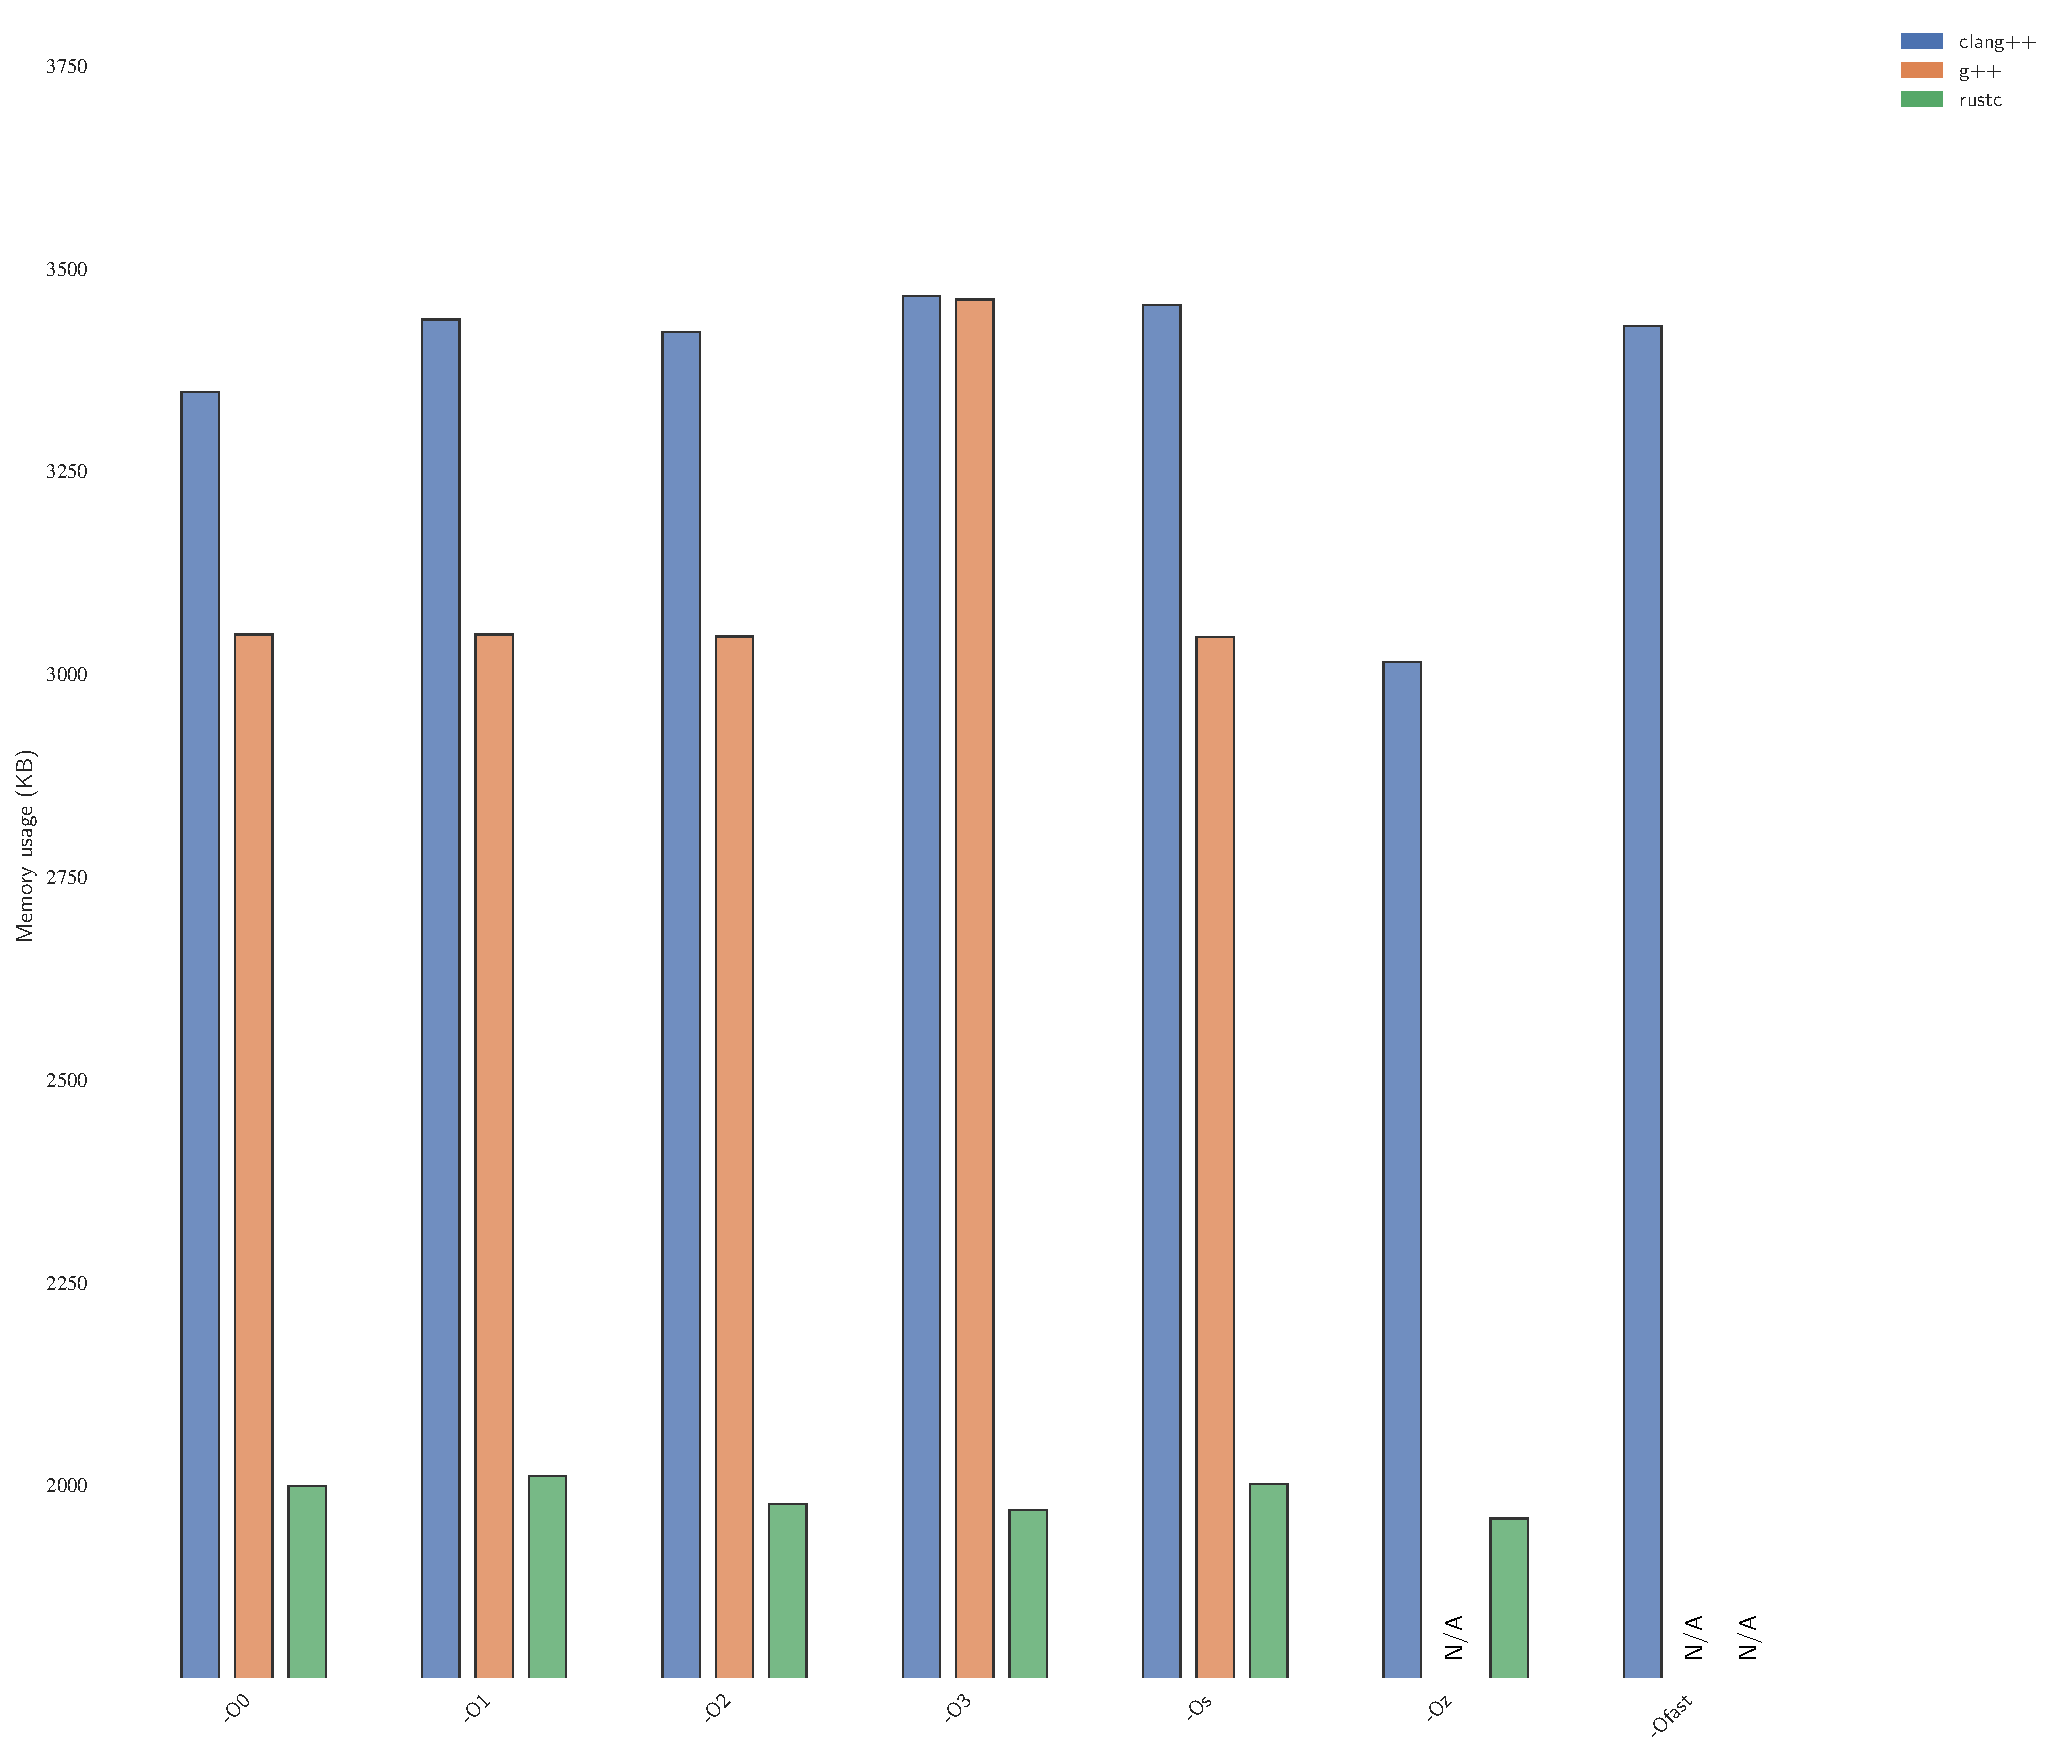
\includegraphics[width=\linewidth]{Gráficas/Gráficas_por_medida_seguridad/pie/enabled/Memory_usage_KB.pdf}
      \label{fig:Gráficas_gráficas_por_medida_seguridad_pie_enabled_memory_usage_kb}
    }
  \end{minipage}
  \hfill
  \begin{minipage}{0.48\textwidth}
    \centering
    \subfloat[Tiempo (ms)]{
      
\includegraphics[width=\linewidth]{Gráficas/Gráficas_por_medida_seguridad/pie/enabled/Time_ms.pdf}
      \label{fig:Gráficas_gráficas_por_medida_seguridad_pie_enabled_time_ms}
    }
  \end{minipage}

\end{figure}
\newpage

% === Gráficas_por_medida_seguridad/relro ===
\subsection*{RELRO}
\begin{figure}[htbp]
  \centering
  \caption{Resultados de compilación con optimización RELRO}
  \vspace{0.5cm}

  \begin{minipage}{0.48\textwidth}
    \centering
    \subfloat[Tamaño del archivo (KB)]{
      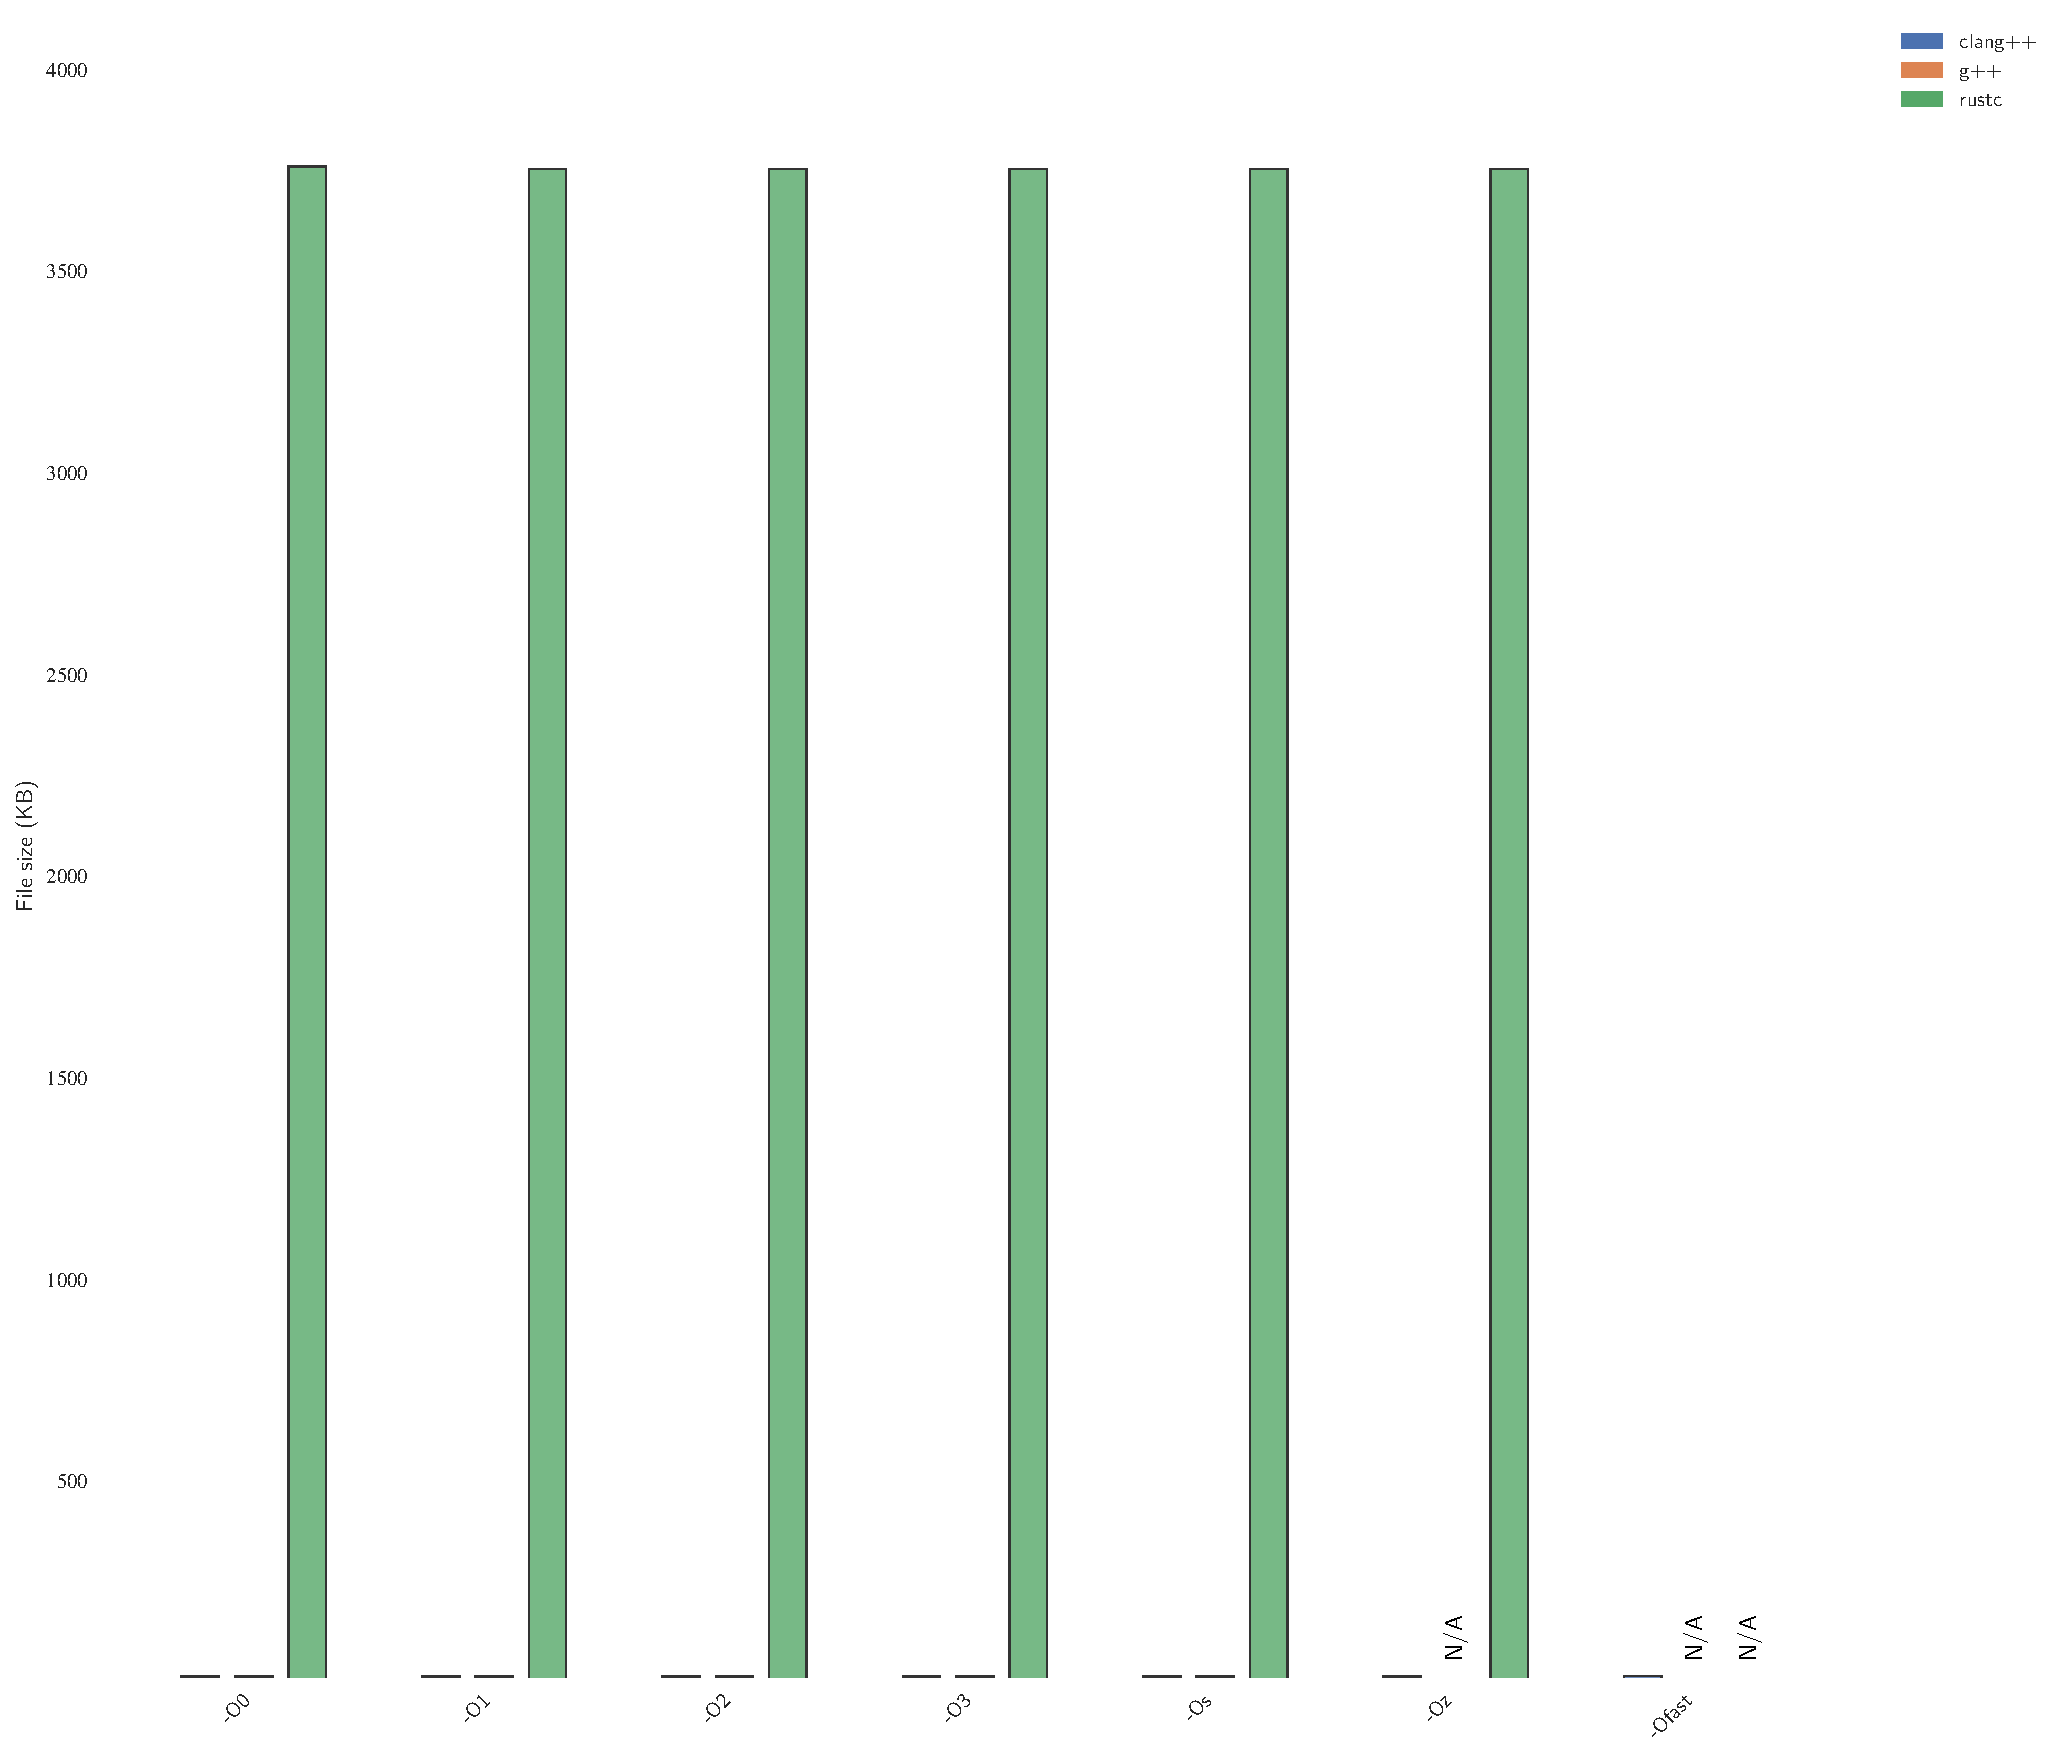
\includegraphics[width=\linewidth]{Gráficas/Gráficas_por_medida_seguridad/relro/File_size_KB.pdf}
      \label{fig:Gráficas_gráficas_por_medida_seguridad_relro_file_size_kb}
    }
  \end{minipage}
  \hfill
  \begin{minipage}{0.48\textwidth}
    \centering
    \subfloat[Funciones fortificadas (\%)]{
      \includegraphics[width=\linewidth]{Gráficas/Gráficas_por_medida_seguridad/relro/Fortified_Functions.pdf}
      \label{fig:Gráficas_gráficas_por_medida_seguridad_relro_fortified_functions}
    }
  \end{minipage}


  \vspace{1cm}

  \begin{minipage}{0.48\textwidth}
    \centering
    \subfloat[Uso de memoria (KB)]{
      
\includegraphics[width=\linewidth]{Gráficas/Gráficas_por_medida_seguridad/relro/Memory_usage_KB.pdf}
      \label{fig:Gráficas_gráficas_por_medida_seguridad_relro_memory_usage_kb}
    }
  \end{minipage}
  \hfill
  \begin{minipage}{0.48\textwidth}
    \centering
    \subfloat[Tiempo (ms)]{
      
\includegraphics[width=\linewidth]{Gráficas/Gráficas_por_medida_seguridad/relro/Time_ms.pdf}
      \label{fig:Gráficas_gráficas_por_medida_seguridad_relro_time_ms}
    }
  \end{minipage}

\end{figure}
\newpage

% === Gráficas_por_medida_seguridad/safe-stack ===
\subsection*{Safe stack}
\begin{figure}[htbp]
  \centering
  \caption{Resultados de compilación con optimización Safe stack}
  \vspace{0.5cm}

  \begin{minipage}{0.48\textwidth}
    \centering
    \subfloat[Tamaño del archivo (KB)]{
      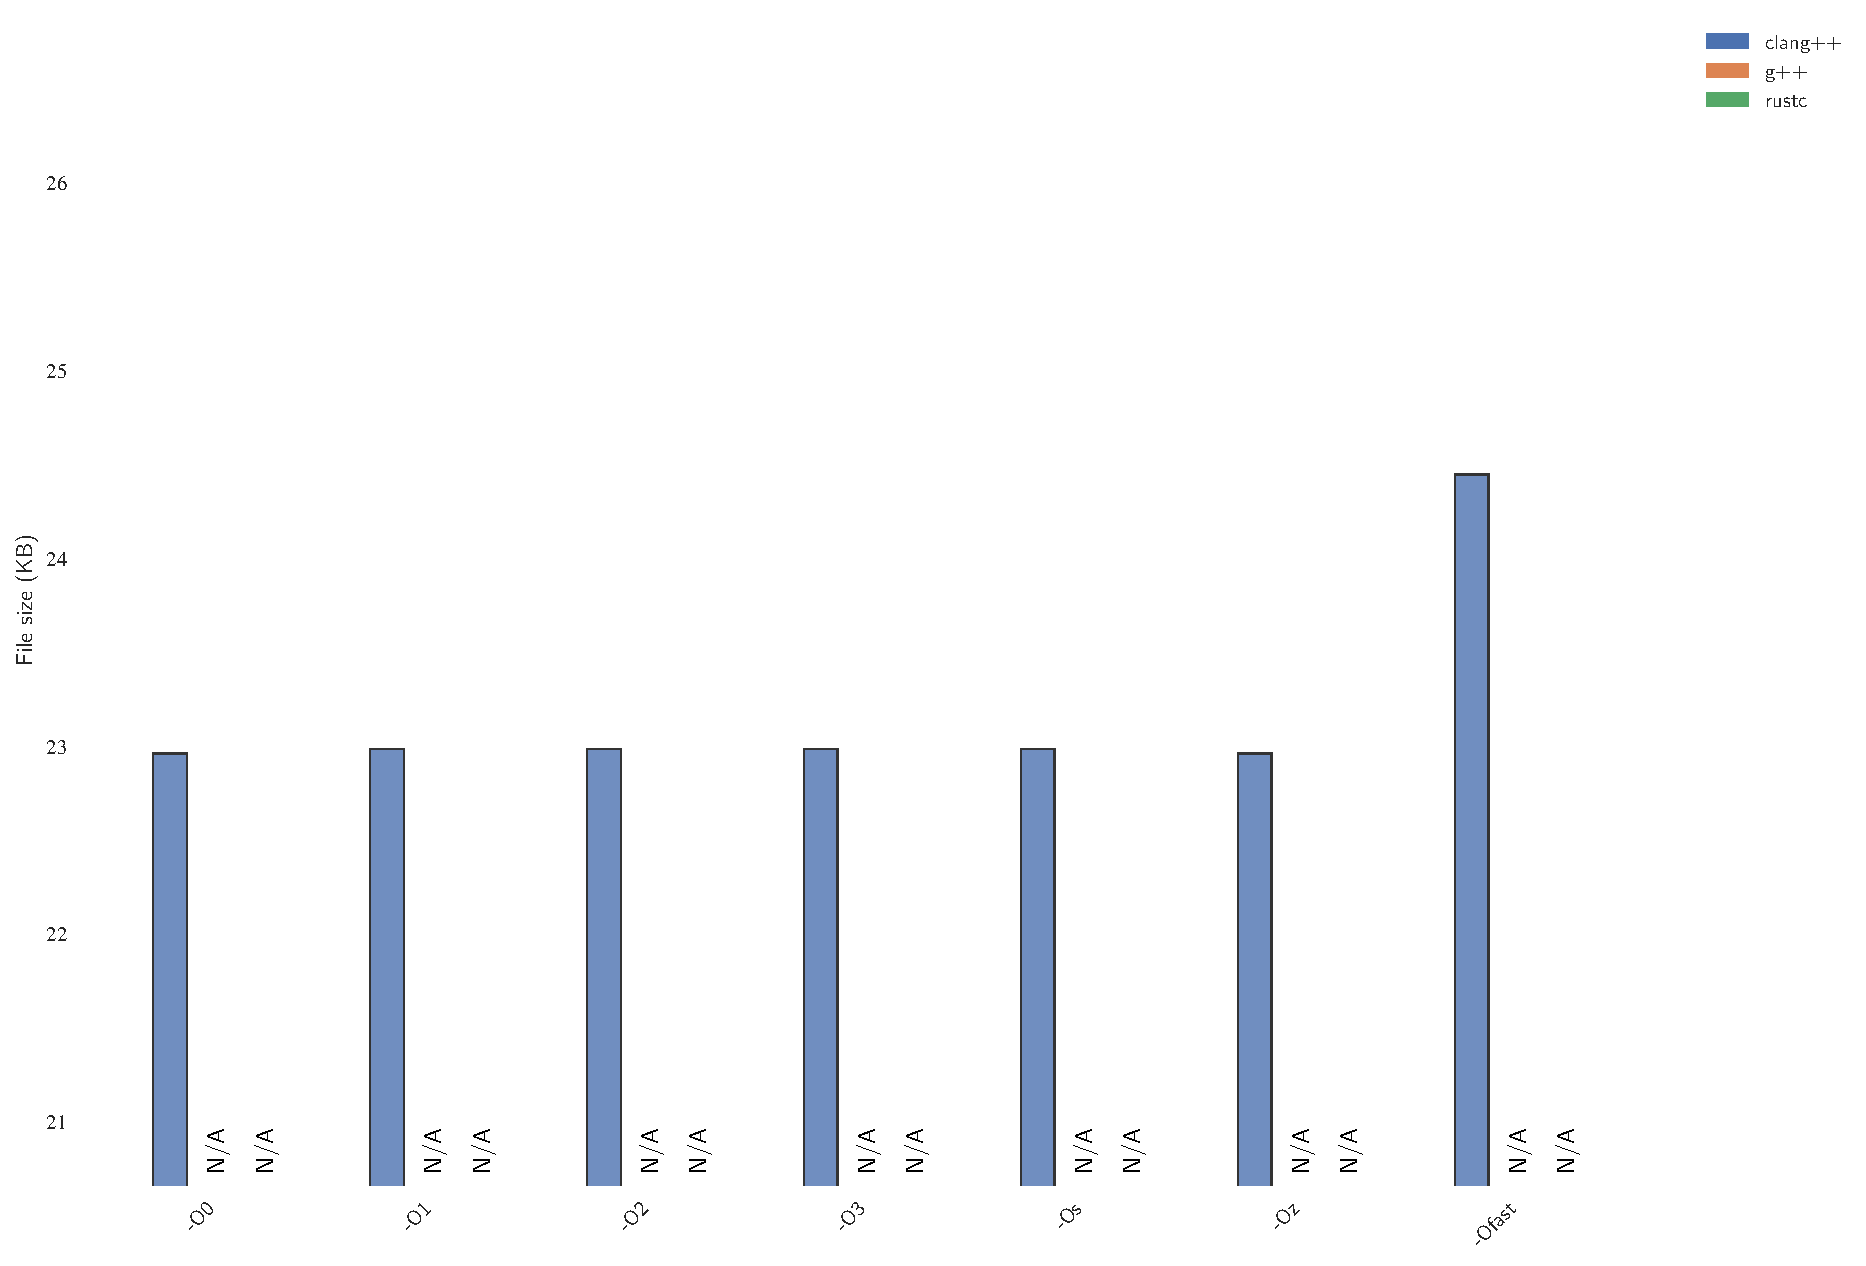
\includegraphics[width=\linewidth]{Gráficas/Gráficas_por_medida_seguridad/safe-stack/File_size_KB.pdf}
      \label{fig:Gráficas_gráficas_por_medida_seguridad_safe_stack_file_size_kb}
    }
  \end{minipage}
  \hfill
  \begin{minipage}{0.48\textwidth}
    \centering
    \subfloat[Funciones fortificadas (\%)]{
      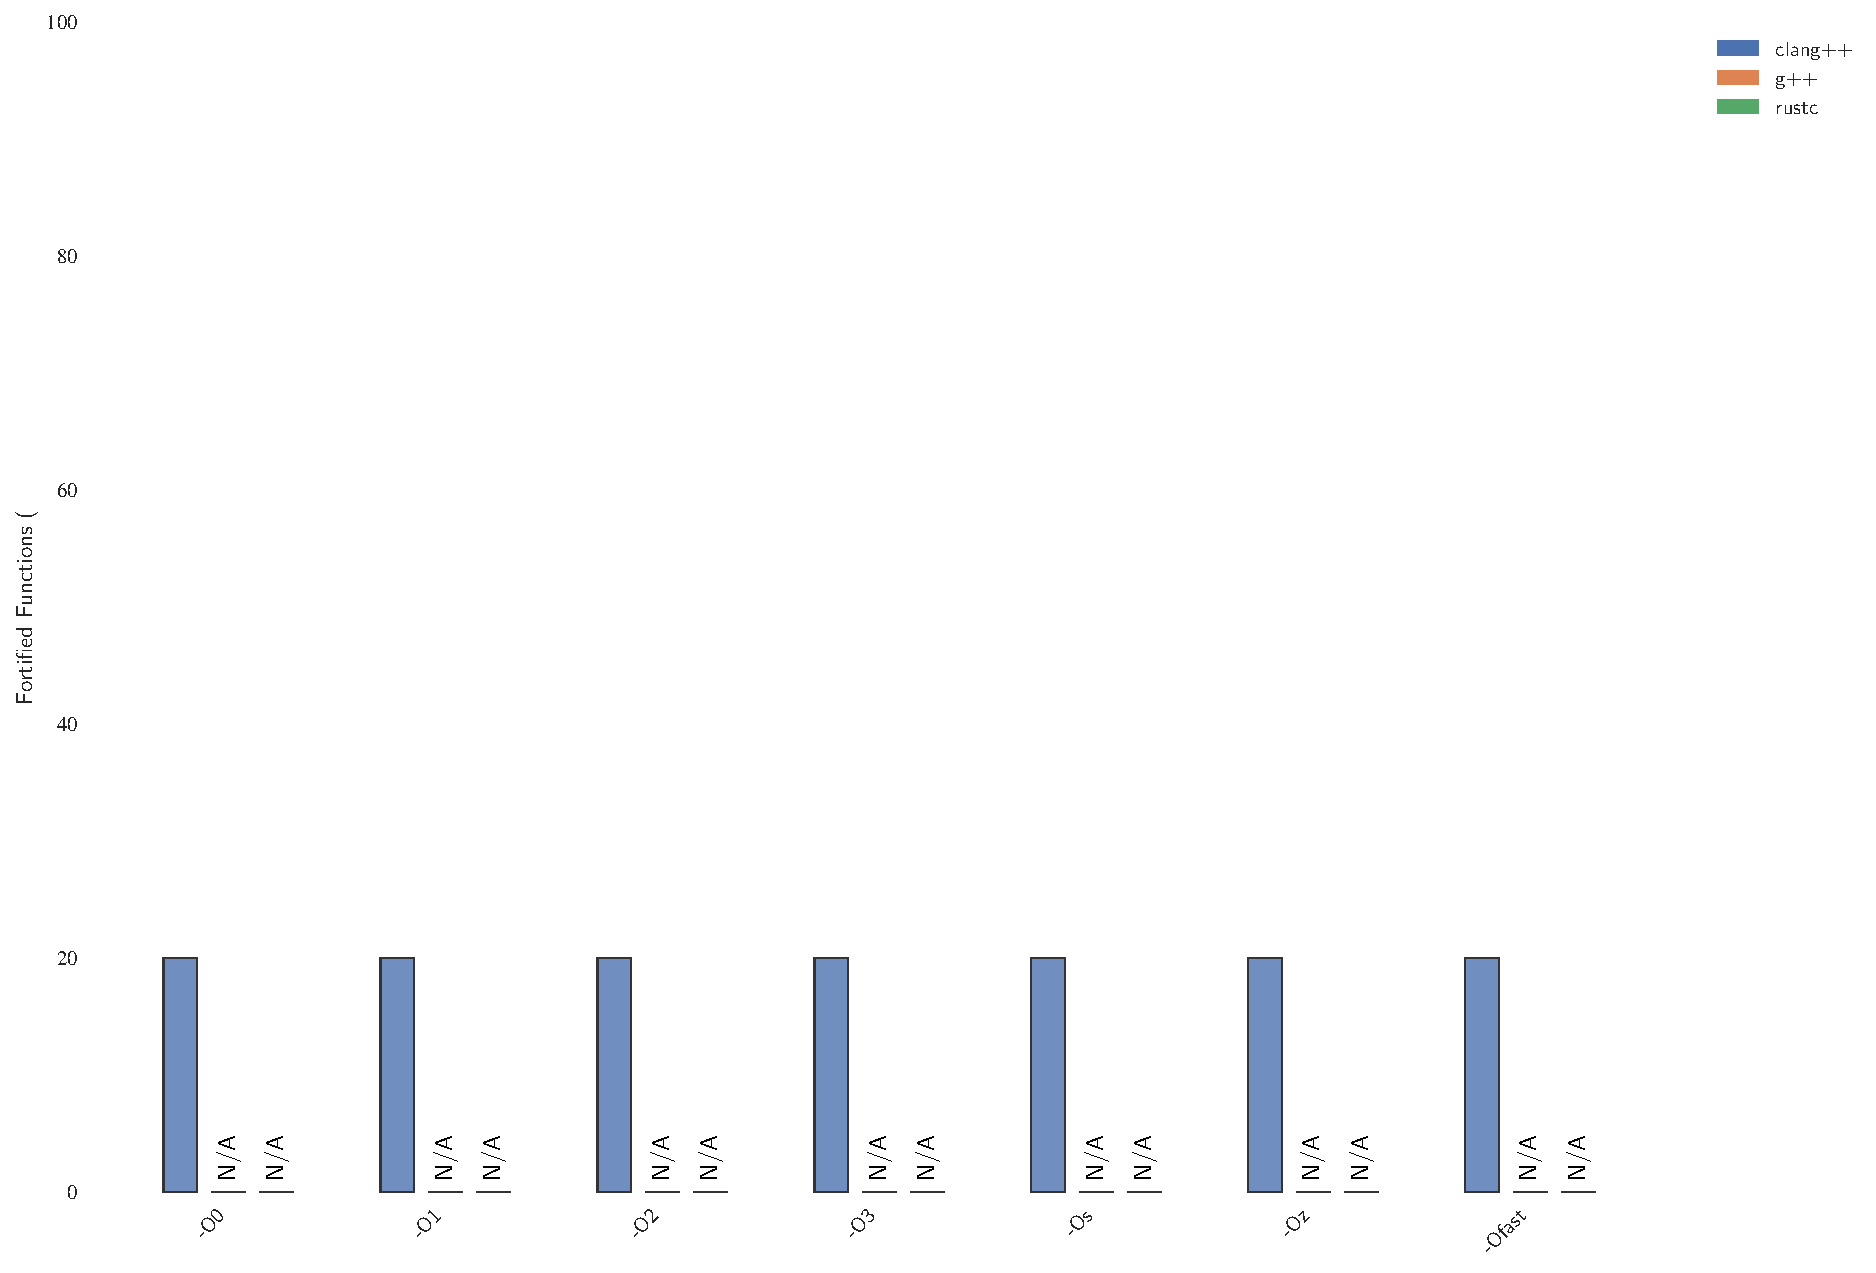
\includegraphics[width=\linewidth]{Gráficas/Gráficas_por_medida_seguridad/safe-stack/Fortified_Functions.pdf}
      \label{fig:Gráficas_gráficas_por_medida_seguridad_safe_stack_fortified_functions}
    }
  \end{minipage}


  \vspace{1cm}

  \begin{minipage}{0.48\textwidth}
    \centering
    \subfloat[Uso de memoria (KB)]{
      
\includegraphics[width=\linewidth]{Gráficas/Gráficas_por_medida_seguridad/safe-stack/Memory_usage_KB.pdf}
      \label{fig:Gráficas_gráficas_por_medida_seguridad_safe_stack_memory_usage_kb}
    }
  \end{minipage}
  \hfill
  \begin{minipage}{0.48\textwidth}
    \centering
    \subfloat[Tiempo (ms)]{
      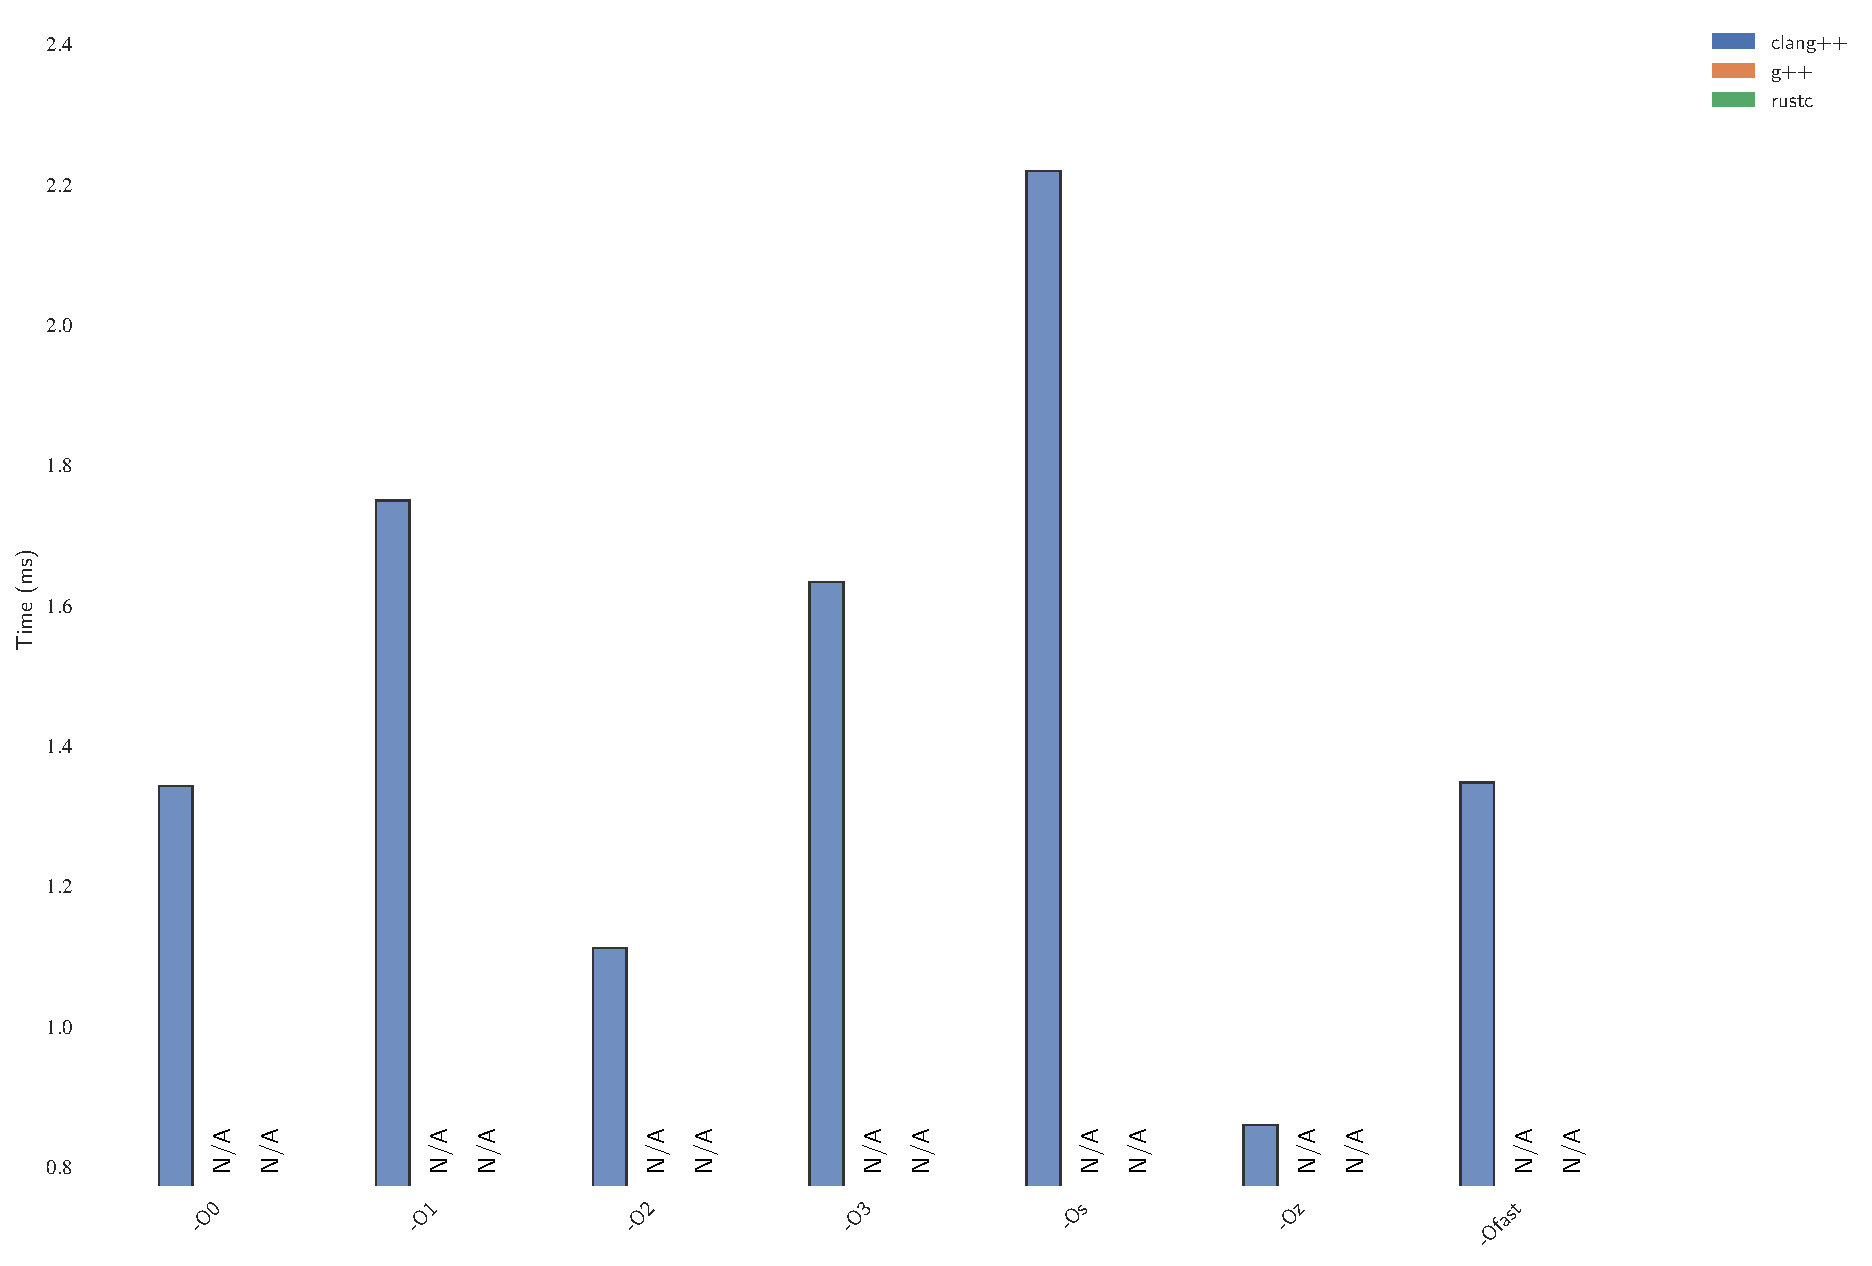
\includegraphics[width=\linewidth]{Gráficas/Gráficas_por_medida_seguridad/safe-stack/Time_ms.pdf}
      \label{fig:Gráficas_gráficas_por_medida_seguridad_safe_stack_time_ms}
    }
  \end{minipage}

\end{figure}
\newpage

% === Gráficas_por_medida_seguridad/sanitizers/address ===
\subsection*{Sanitizadores / AddressSanitizer}
\begin{figure}[htbp]
  \centering
  \caption{Resultados para Sanitizadores (AddressSanitizer)}
  \vspace{0.5cm}

  \begin{minipage}{0.48\textwidth}
    \centering
    \subfloat[Tamaño del archivo (KB)]{
      
\includegraphics[width=\linewidth]{Gráficas/Gráficas_por_medida_seguridad/sanitizers/address/File_size_KB.pdf}
      \label{fig:Gráficas_gráficas_por_medida_seguridad_sanitizers_address_file_size_kb}
    }
  \end{minipage}
  \hfill
  \begin{minipage}{0.48\textwidth}
    \centering
    \subfloat[Funciones fortificadas (\%)]{
      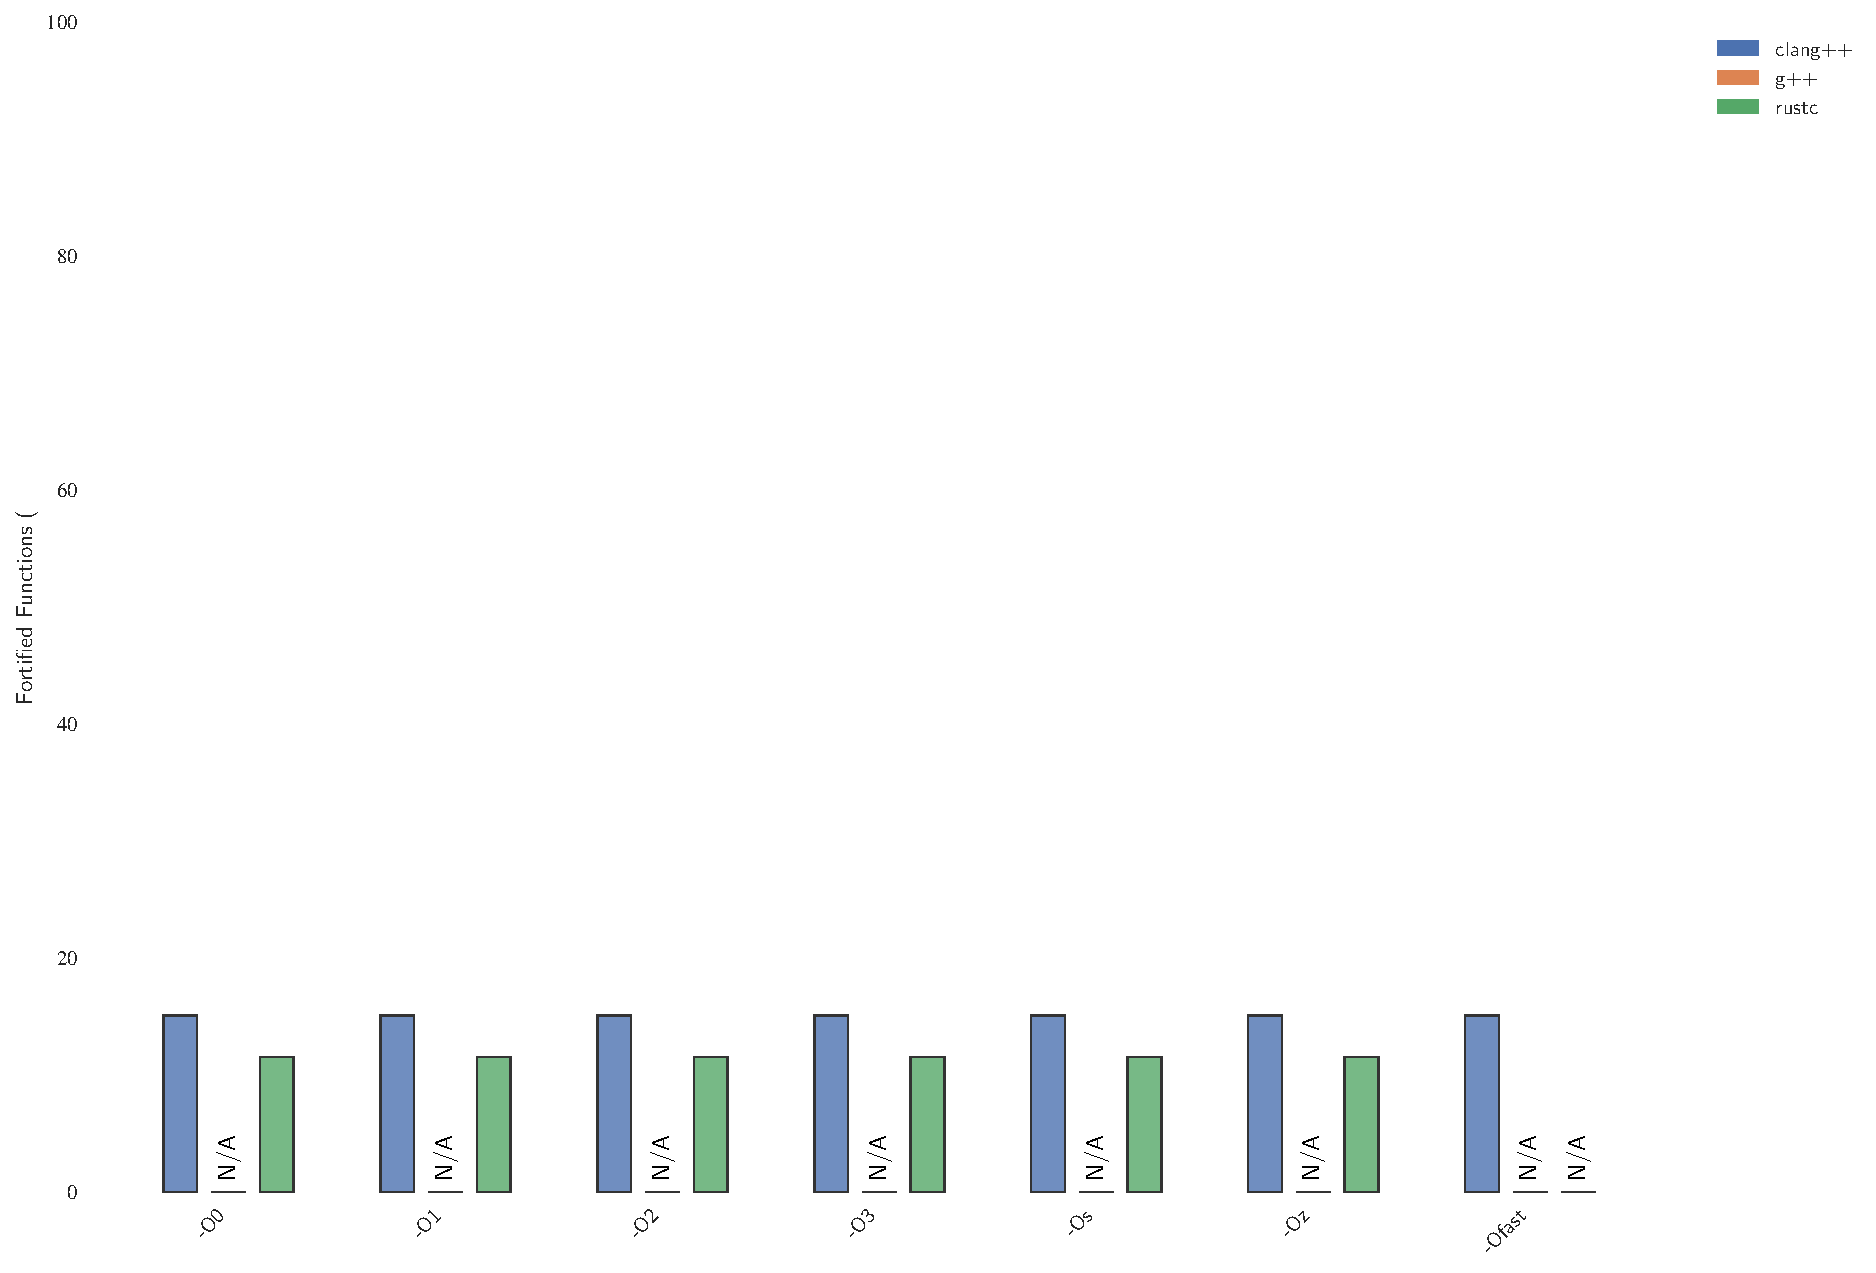
\includegraphics[width=\linewidth]{Gráficas/Gráficas_por_medida_seguridad/sanitizers/address/Fortified_Functions.pdf}
      \label{fig:Gráficas_gráficas_por_medida_seguridad_sanitizers_address_fortified_functions}
    }
  \end{minipage}


  \vspace{1cm}

  \begin{minipage}{0.48\textwidth}
    \centering
    \subfloat[Uso de memoria (KB)]{
      
\includegraphics[width=\linewidth]{Gráficas/Gráficas_por_medida_seguridad/sanitizers/address/Memory_usage_KB.pdf}
      \label{fig:Gráficas_gráficas_por_medida_seguridad_sanitizers_address_memory_usage_kb}
    }
  \end{minipage}
  \hfill
  \begin{minipage}{0.48\textwidth}
    \centering
    \subfloat[Tiempo (ms)]{
      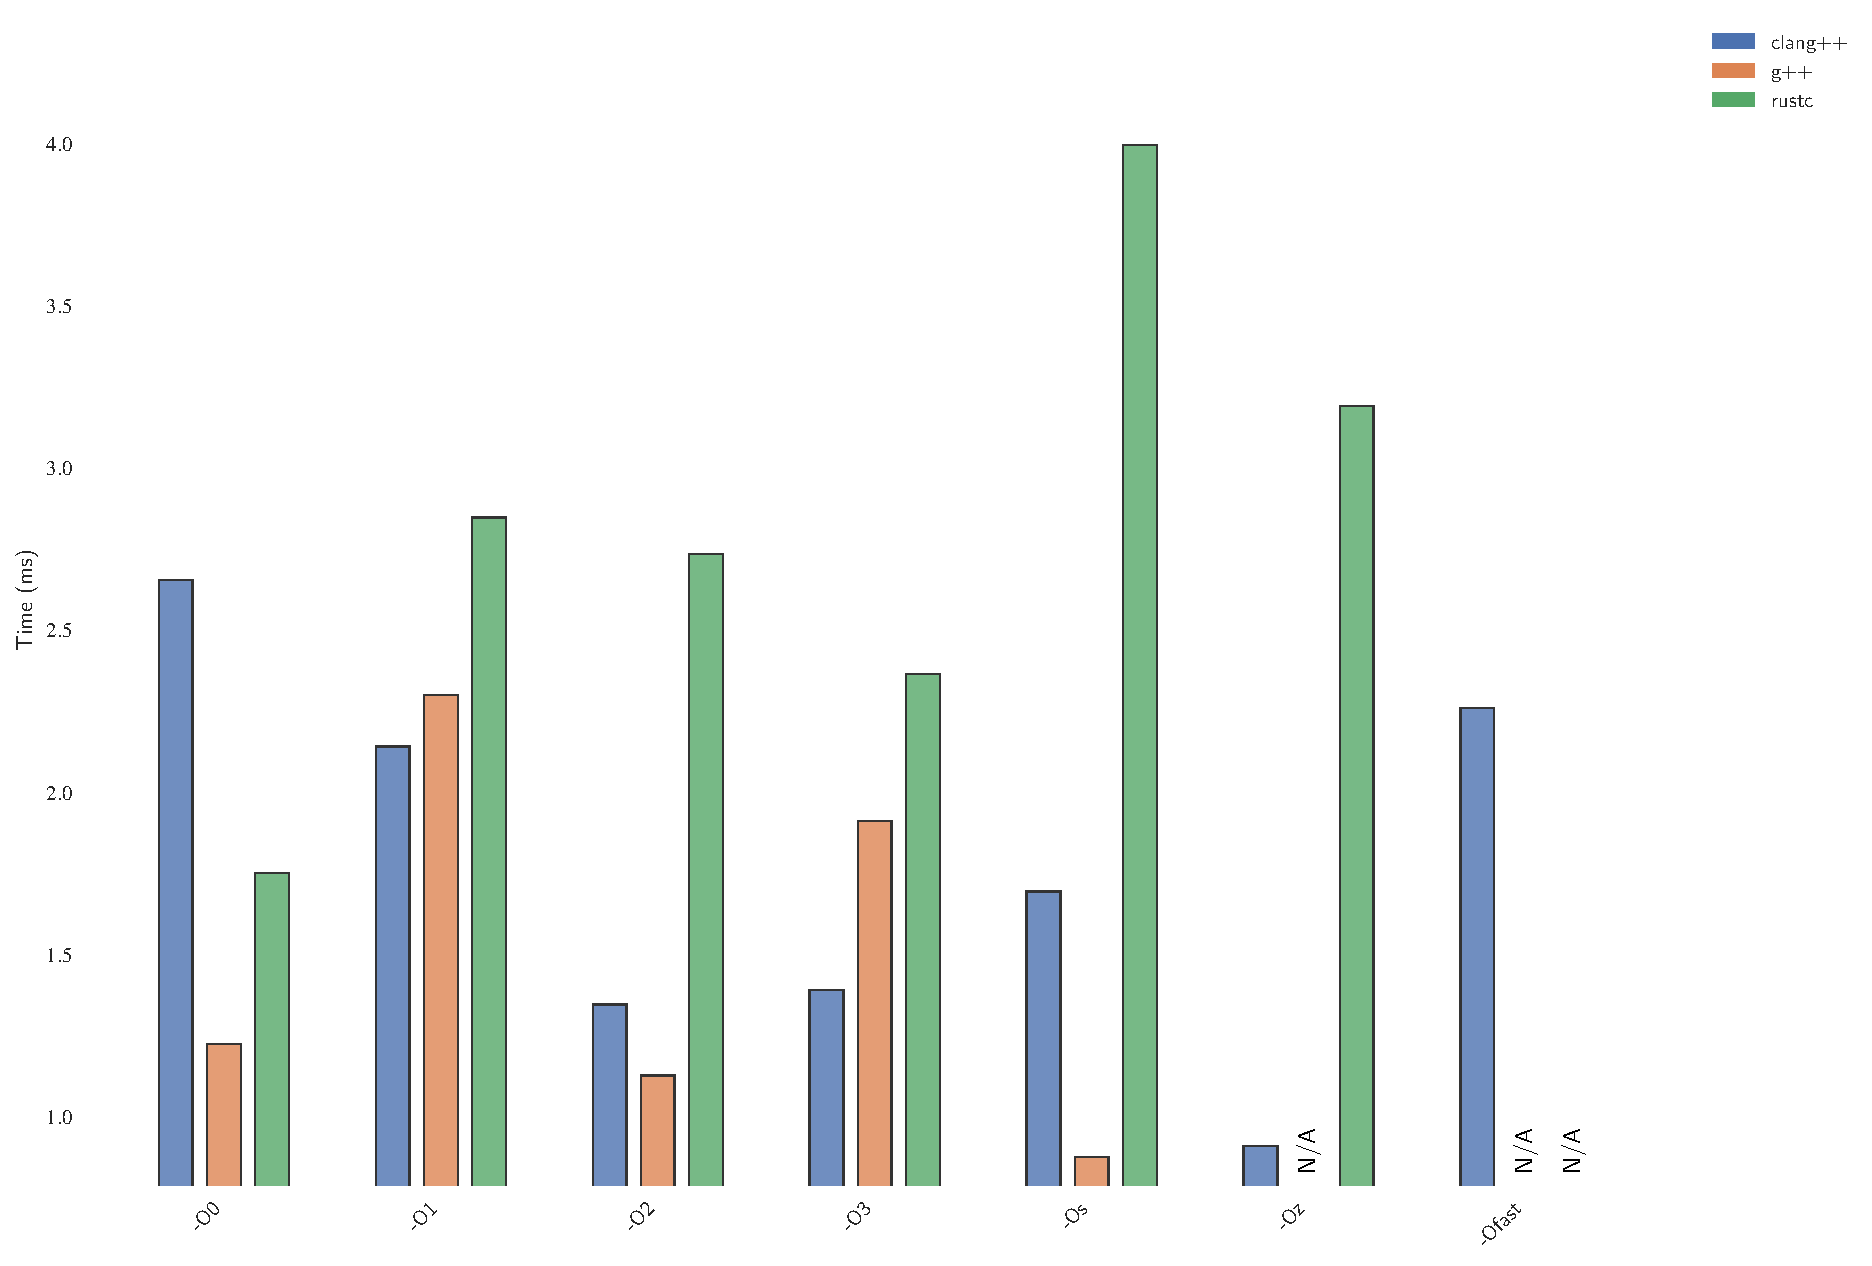
\includegraphics[width=\linewidth]{Gráficas/Gráficas_por_medida_seguridad/sanitizers/address/Time_ms.pdf}
      \label{fig:Gráficas_gráficas_por_medida_seguridad_sanitizers_address_time_ms}
    }
  \end{minipage}

\end{figure}
\newpage

% === Gráficas_por_medida_seguridad/sanitizers/undefined ===
\subsection*{Sanitizadores / UndefinedSanitizer}
\begin{figure}[htbp]
  \centering
  \caption{Resultados para Sanitizadores (UndefinedSanitizer)}
  \vspace{0.5cm}

  \begin{minipage}{0.48\textwidth}
    \centering
    \subfloat[Tamaño del archivo (KB)]{
      
\includegraphics[width=\linewidth]{Gráficas/Gráficas_por_medida_seguridad/sanitizers/undefined/File_size_KB.pdf}
      \label{fig:Gráficas_gráficas_por_medida_seguridad_sanitizers_undefined_file_size_kb}
    }
  \end{minipage}
  \hfill
  \begin{minipage}{0.48\textwidth}
    \centering
    \subfloat[Funciones fortificadas (\%)]{
      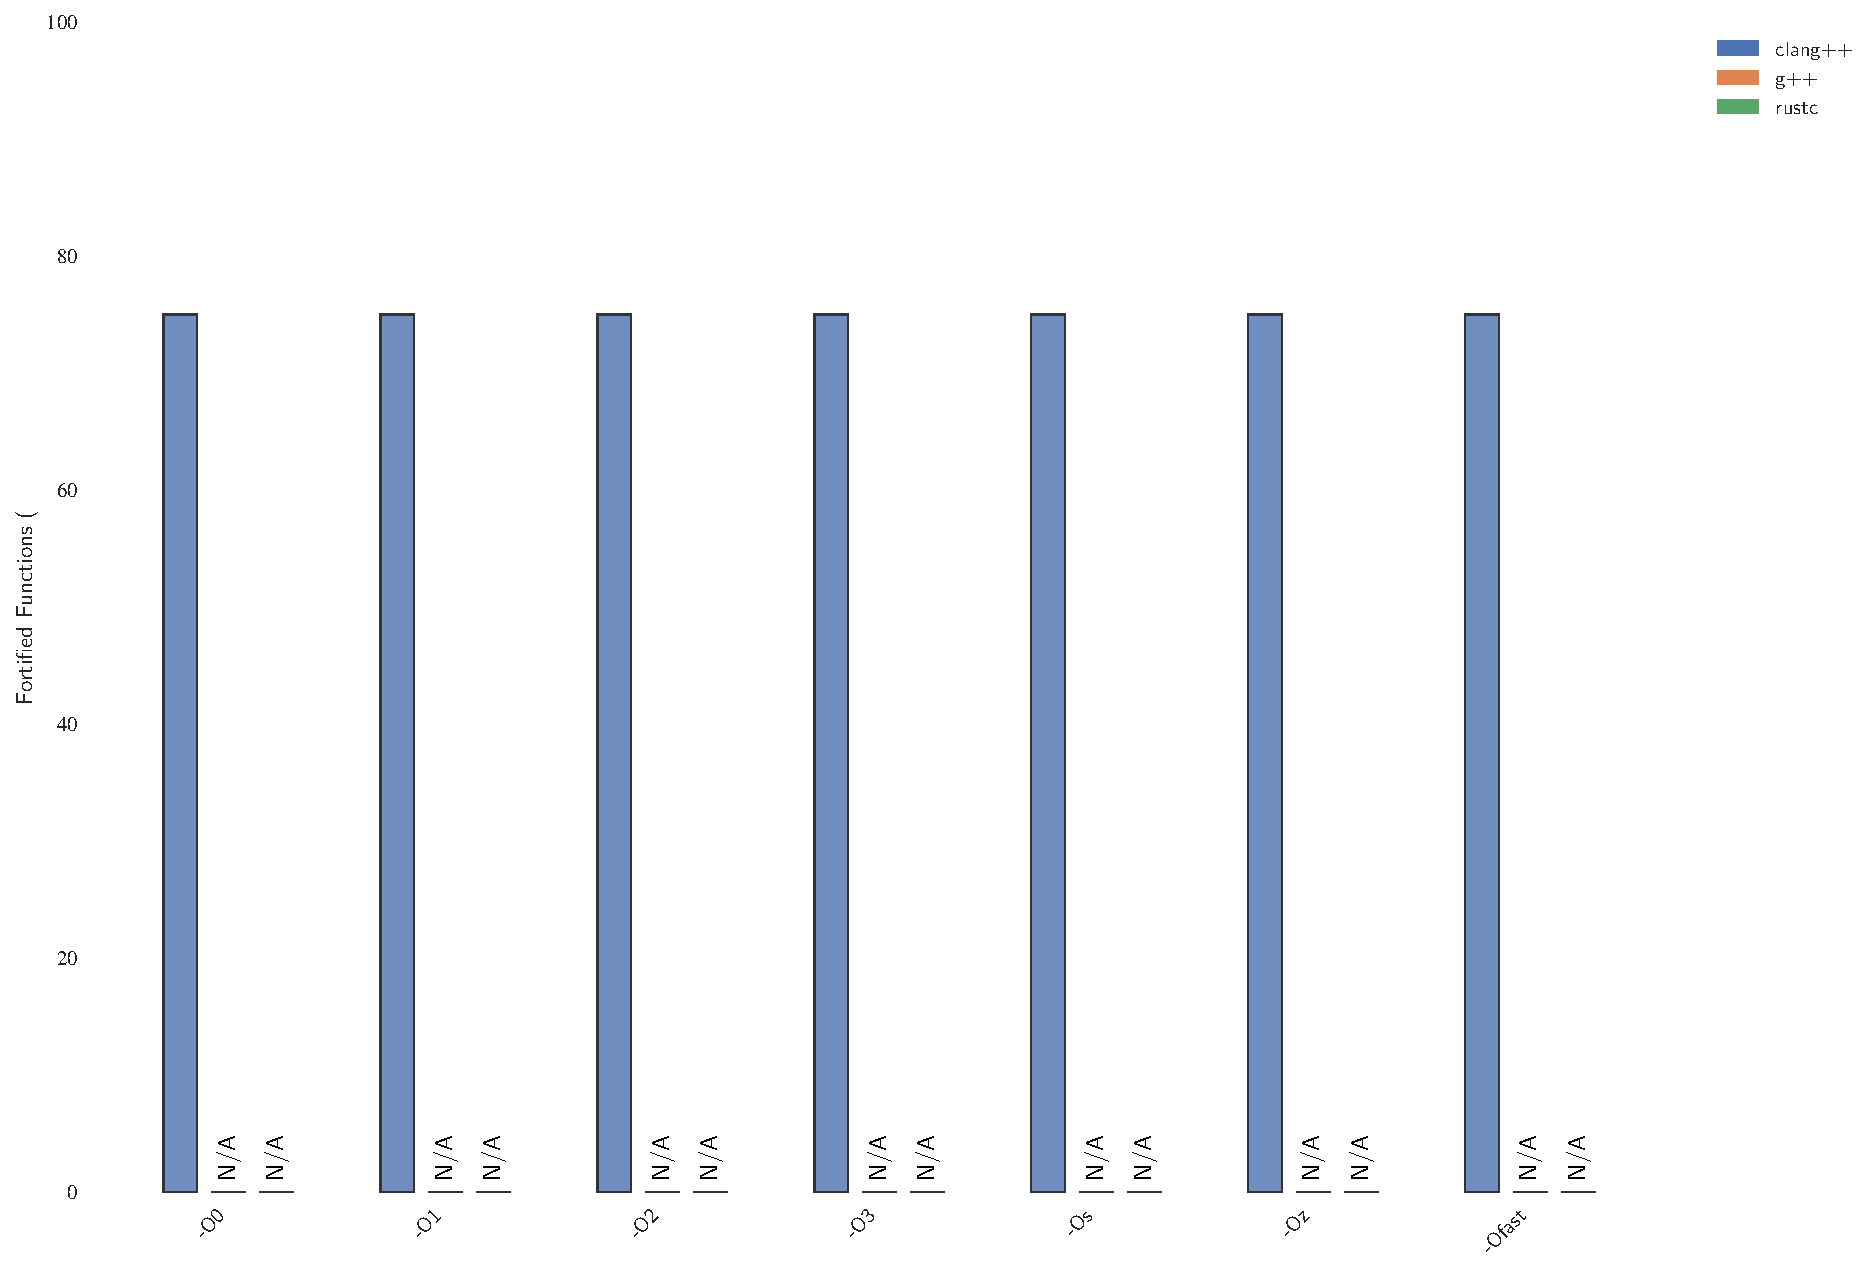
\includegraphics[width=\linewidth]{Gráficas/Gráficas_por_medida_seguridad/sanitizers/undefined/Fortified_Functions.pdf}
      \label{fig:Gráficas_gráficas_por_medida_seguridad_sanitizers_undefined_fortified_functions}
    }
  \end{minipage}


  \vspace{1cm}

  \begin{minipage}{0.48\textwidth}
    \centering
    \subfloat[Uso de memoria (KB)]{
      
\includegraphics[width=\linewidth]{Gráficas/Gráficas_por_medida_seguridad/sanitizers/undefined/Memory_usage_KB.pdf}
      \label{fig:Gráficas_gráficas_por_medida_seguridad_sanitizers_undefined_memory_usage_kb}
    }
  \end{minipage}
  \hfill
  \begin{minipage}{0.48\textwidth}
    \centering
    \subfloat[Tiempo (ms)]{
      
\includegraphics[width=\linewidth]{Gráficas/Gráficas_por_medida_seguridad/sanitizers/undefined/Time_ms.pdf}
      \label{fig:Gráficas_gráficas_por_medida_seguridad_sanitizers_undefined_time_ms}
    }
  \end{minipage}

\end{figure}
\newpage

% === Gráficas_por_medida_seguridad/stack-protection/all ===
\subsection*{Stack protector / all}
\begin{figure}[htbp]
  \centering
  \caption{Resultados para Stack protector (all)}
  \vspace{0.5cm}

  \begin{minipage}{0.48\textwidth}
    \centering
    \subfloat[Tamaño del archivo (KB)]{
      
\includegraphics[width=\linewidth]{Gráficas/Gráficas_por_medida_seguridad/stack-protection/all/File_size_KB.pdf}
      \label{fig:Gráficas_gráficas_por_medida_seguridad_stack_protection_all_file_size_kb}
    }
  \end{minipage}
  \hfill
  \begin{minipage}{0.48\textwidth}
    \centering
    \subfloat[Funciones fortificadas (\%)]{
      \includegraphics[width=\linewidth]{Gráficas/Gráficas_por_medida_seguridad/stack-protection/all/Fortified_Functions.pdf}
      \label{fig:Gráficas_gráficas_por_medida_seguridad_stack_protection_all_fortified_functions}
    }
  \end{minipage}


  \vspace{1cm}

  \begin{minipage}{0.48\textwidth}
    \centering
    \subfloat[Uso de memoria (KB)]{
      
\includegraphics[width=\linewidth]{Gráficas/Gráficas_por_medida_seguridad/stack-protection/all/Memory_usage_KB.pdf}
      \label{fig:Gráficas_gráficas_por_medida_seguridad_stack_protection_all_memory_usage_kb}
    }
  \end{minipage}
  \hfill
  \begin{minipage}{0.48\textwidth}
    \centering
    \subfloat[Tiempo (ms)]{
      
\includegraphics[width=\linewidth]{Gráficas/Gráficas_por_medida_seguridad/stack-protection/all/Time_ms.pdf}
      \label{fig:Gráficas_gráficas_por_medida_seguridad_stack_protection_all_time_ms}
    }
  \end{minipage}

\end{figure}
\newpage

% === Gráficas_por_medida_seguridad/stack-protection/basic ===
\subsection*{Stack protector / basic}
\begin{figure}[htbp]
  \centering
  \caption{Resultados para Stack protector (basic)}
  \vspace{0.5cm}

  \begin{minipage}{0.48\textwidth}
    \centering
    \subfloat[Tamaño del archivo (KB)]{
      
\includegraphics[width=\linewidth]{Gráficas/Gráficas_por_medida_seguridad/stack-protection/basic/File_size_KB.pdf}
      \label{fig:Gráficas_gráficas_por_medida_seguridad_stack_protection_basic_file_size_kb}
    }
  \end{minipage}
  \hfill
  \begin{minipage}{0.48\textwidth}
    \centering
    \subfloat[Funciones fortificadas (\%)]{
      \includegraphics[width=\linewidth]{Gráficas/Gráficas_por_medida_seguridad/stack-protection/basic/Fortified_Functions.pdf}
      \label{fig:Gráficas_gráficas_por_medida_seguridad_stack_protection_basic_fortified_functions}
    }
  \end{minipage}


  \vspace{1cm}

  \begin{minipage}{0.48\textwidth}
    \centering
    \subfloat[Uso de memoria (KB)]{
      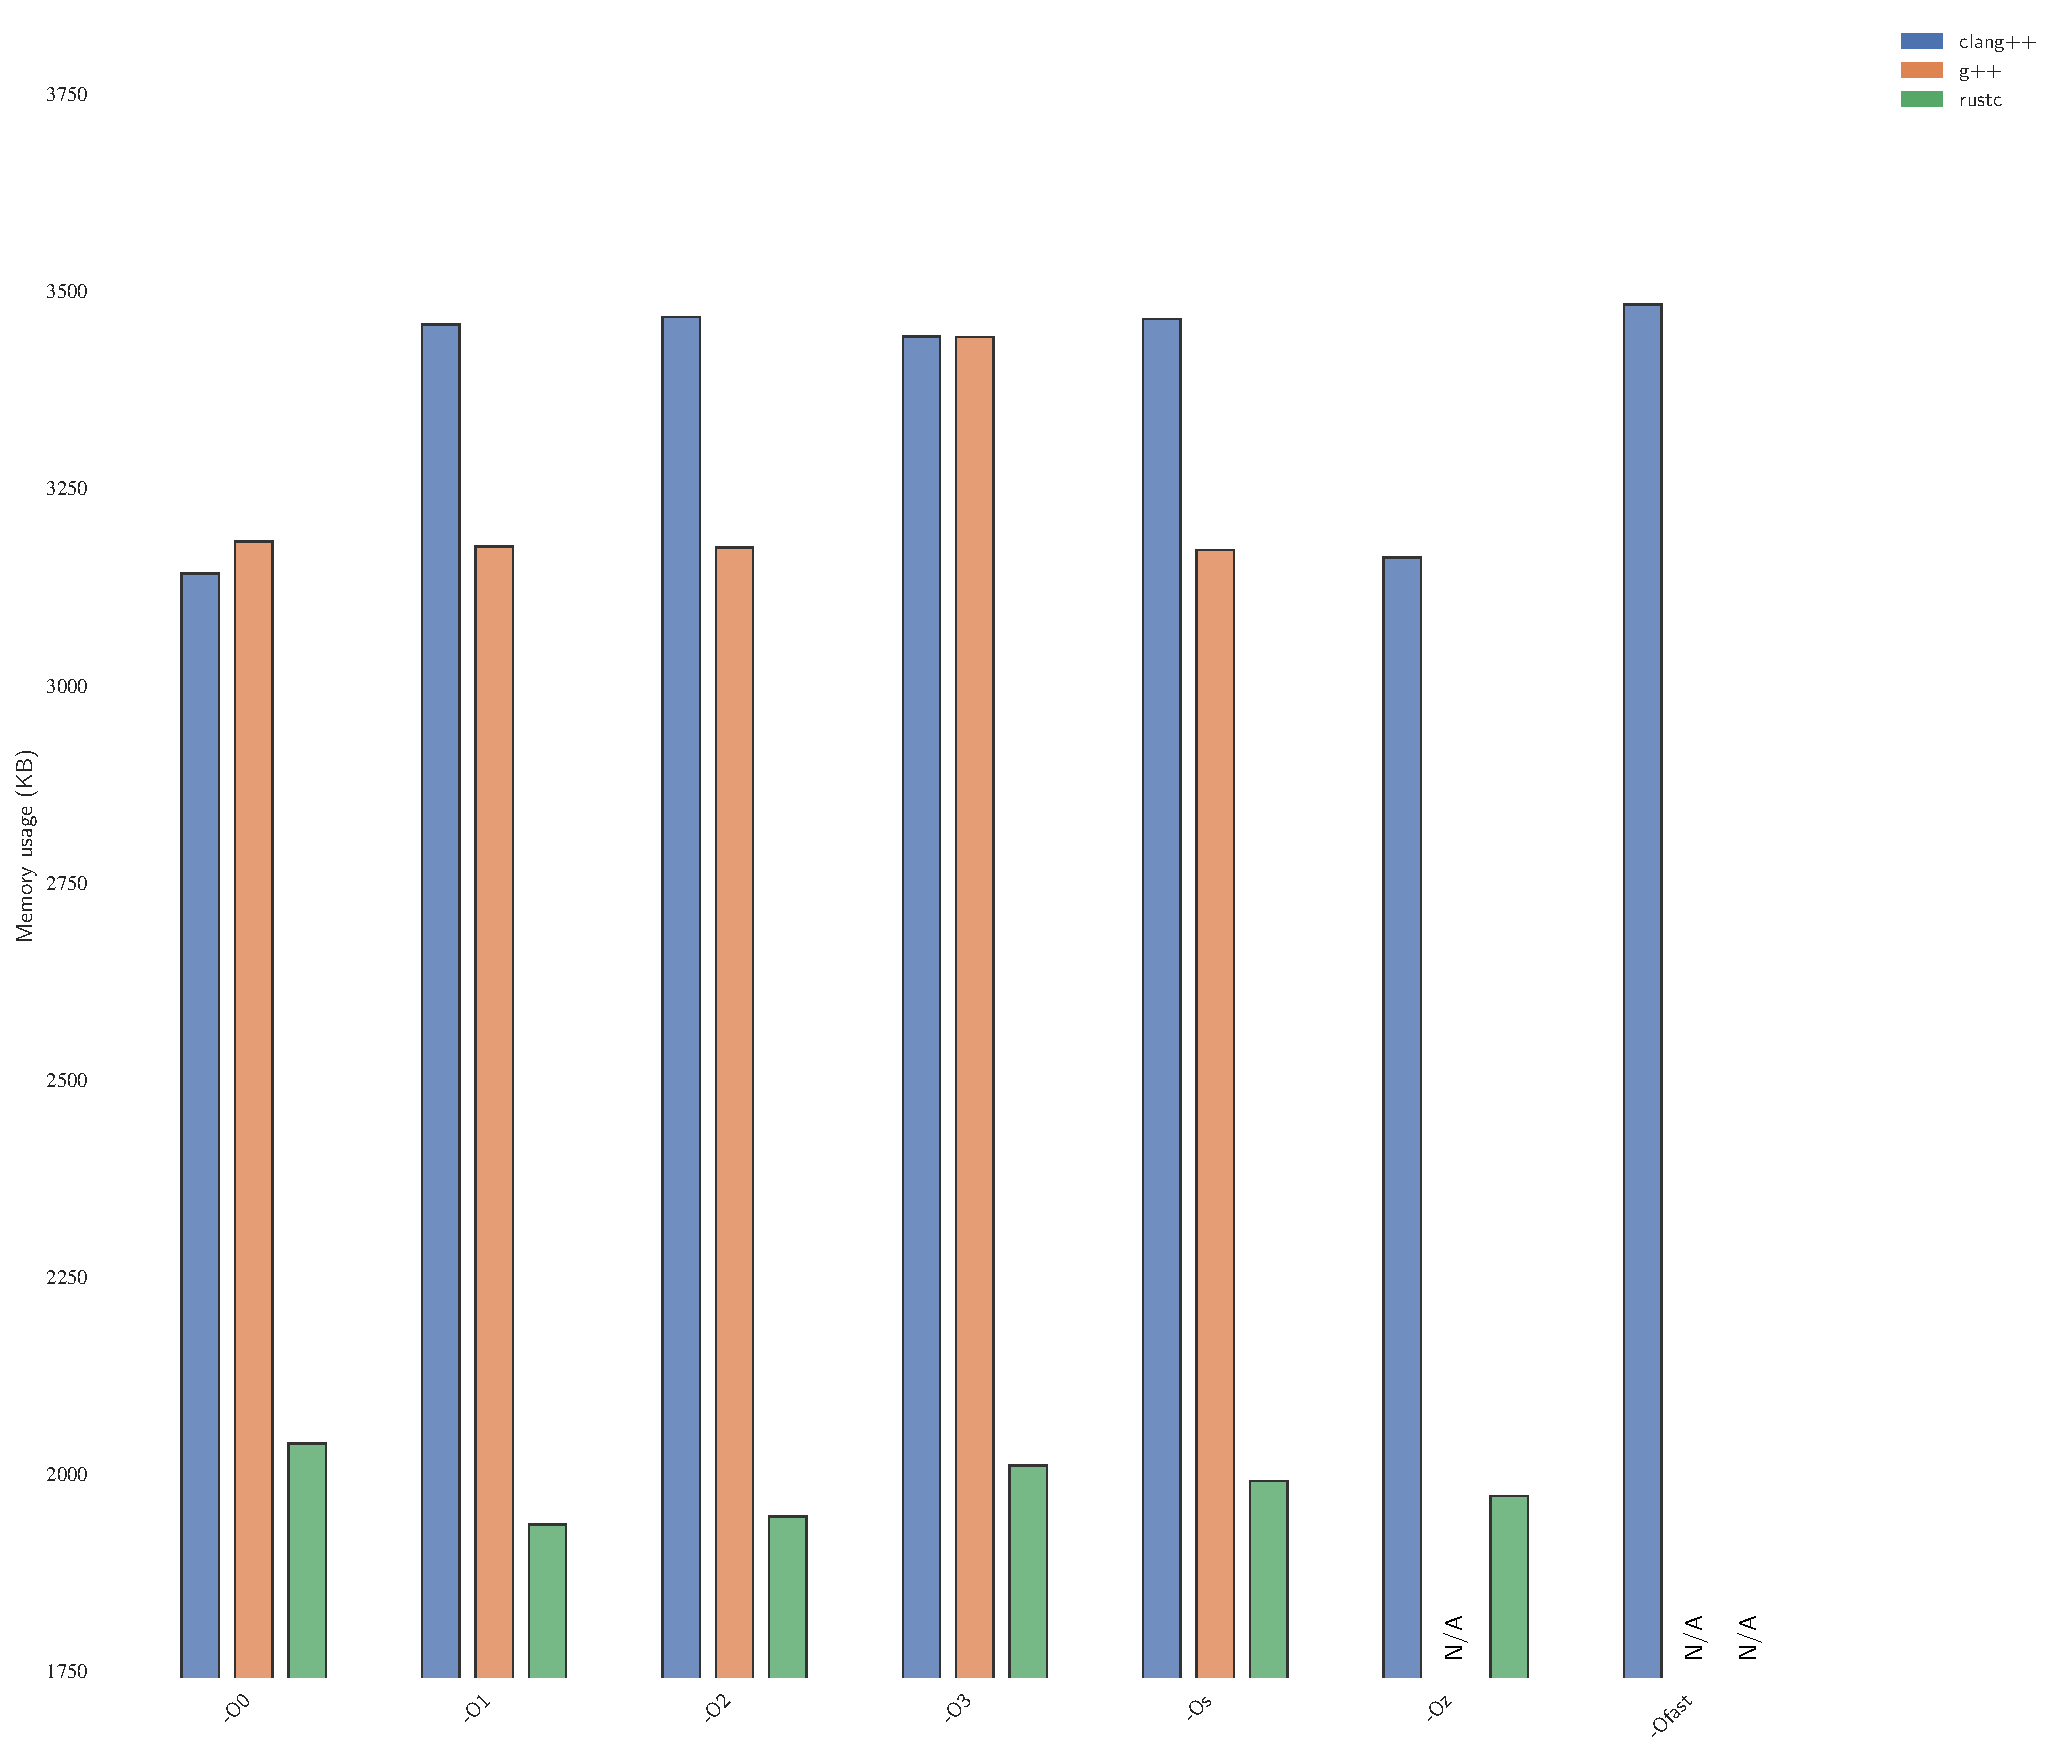
\includegraphics[width=\linewidth]{Gráficas/Gráficas_por_medida_seguridad/stack-protection/basic/Memory_usage_KB.pdf}
      \label{fig:Gráficas_gráficas_por_medida_seguridad_stack_protection_basic_memory_usage_kb}
    }
  \end{minipage}
  \hfill
  \begin{minipage}{0.48\textwidth}
    \centering
    \subfloat[Tiempo (ms)]{
      
\includegraphics[width=\linewidth]{Gráficas/Gráficas_por_medida_seguridad/stack-protection/basic/Time_ms.pdf}
      \label{fig:Gráficas_gráficas_por_medida_seguridad_stack_protection_basic_time_ms}
    }
  \end{minipage}

\end{figure}
\newpage

% === Gráficas_por_medida_seguridad/stack-protection/disabled ===
\subsection*{Stack protector / disabled}
\begin{figure}[htbp]
  \centering
  \caption{Resultados para Stack protector (disabled)}
  \vspace{0.5cm}

  \begin{minipage}{0.48\textwidth}
    \centering
    \subfloat[Tamaño del archivo (KB)]{
      
\includegraphics[width=\linewidth]{Gráficas/Gráficas_por_medida_seguridad/stack-protection/disabled/File_size_KB.pdf}
      \label{fig:Gráficas_gráficas_por_medida_seguridad_stack_protection_disabled_file_size_kb}
    }
  \end{minipage}
  \hfill
  \begin{minipage}{0.48\textwidth}
    \centering
    \subfloat[Funciones fortificadas (\%)]{
      \includegraphics[width=\linewidth]{Gráficas/Gráficas_por_medida_seguridad/stack-protection/disabled/Fortified_Functions.pdf}
      \label{fig:Gráficas_gráficas_por_medida_seguridad_stack_protection_disabled_fortified_functions}
    }
  \end{minipage}


  \vspace{1cm}

  \begin{minipage}{0.48\textwidth}
    \centering
    \subfloat[Uso de memoria (KB)]{
      
\includegraphics[width=\linewidth]{Gráficas/Gráficas_por_medida_seguridad/stack-protection/disabled/Memory_usage_KB.pdf}
      \label{fig:Gráficas_gráficas_por_medida_seguridad_stack_protection_disabled_memory_usage_kb}
    }
  \end{minipage}
  \hfill
  \begin{minipage}{0.48\textwidth}
    \centering
    \subfloat[Tiempo (ms)]{
      
\includegraphics[width=\linewidth]{Gráficas/Gráficas_por_medida_seguridad/stack-protection/disabled/Time_ms.pdf}
      \label{fig:Gráficas_gráficas_por_medida_seguridad_stack_protection_disabled_time_ms}
    }
  \end{minipage}

\end{figure}
\newpage

% === Gráficas_por_medida_seguridad/stack-protection/strong ===
\subsection*{Stack protector / strong}
\begin{figure}[htbp]
  \centering
  \caption{Resultados para Stack protector (strong)}
  \vspace{0.5cm}

  \begin{minipage}{0.48\textwidth}
    \centering
    \subfloat[Tamaño del archivo (KB)]{
      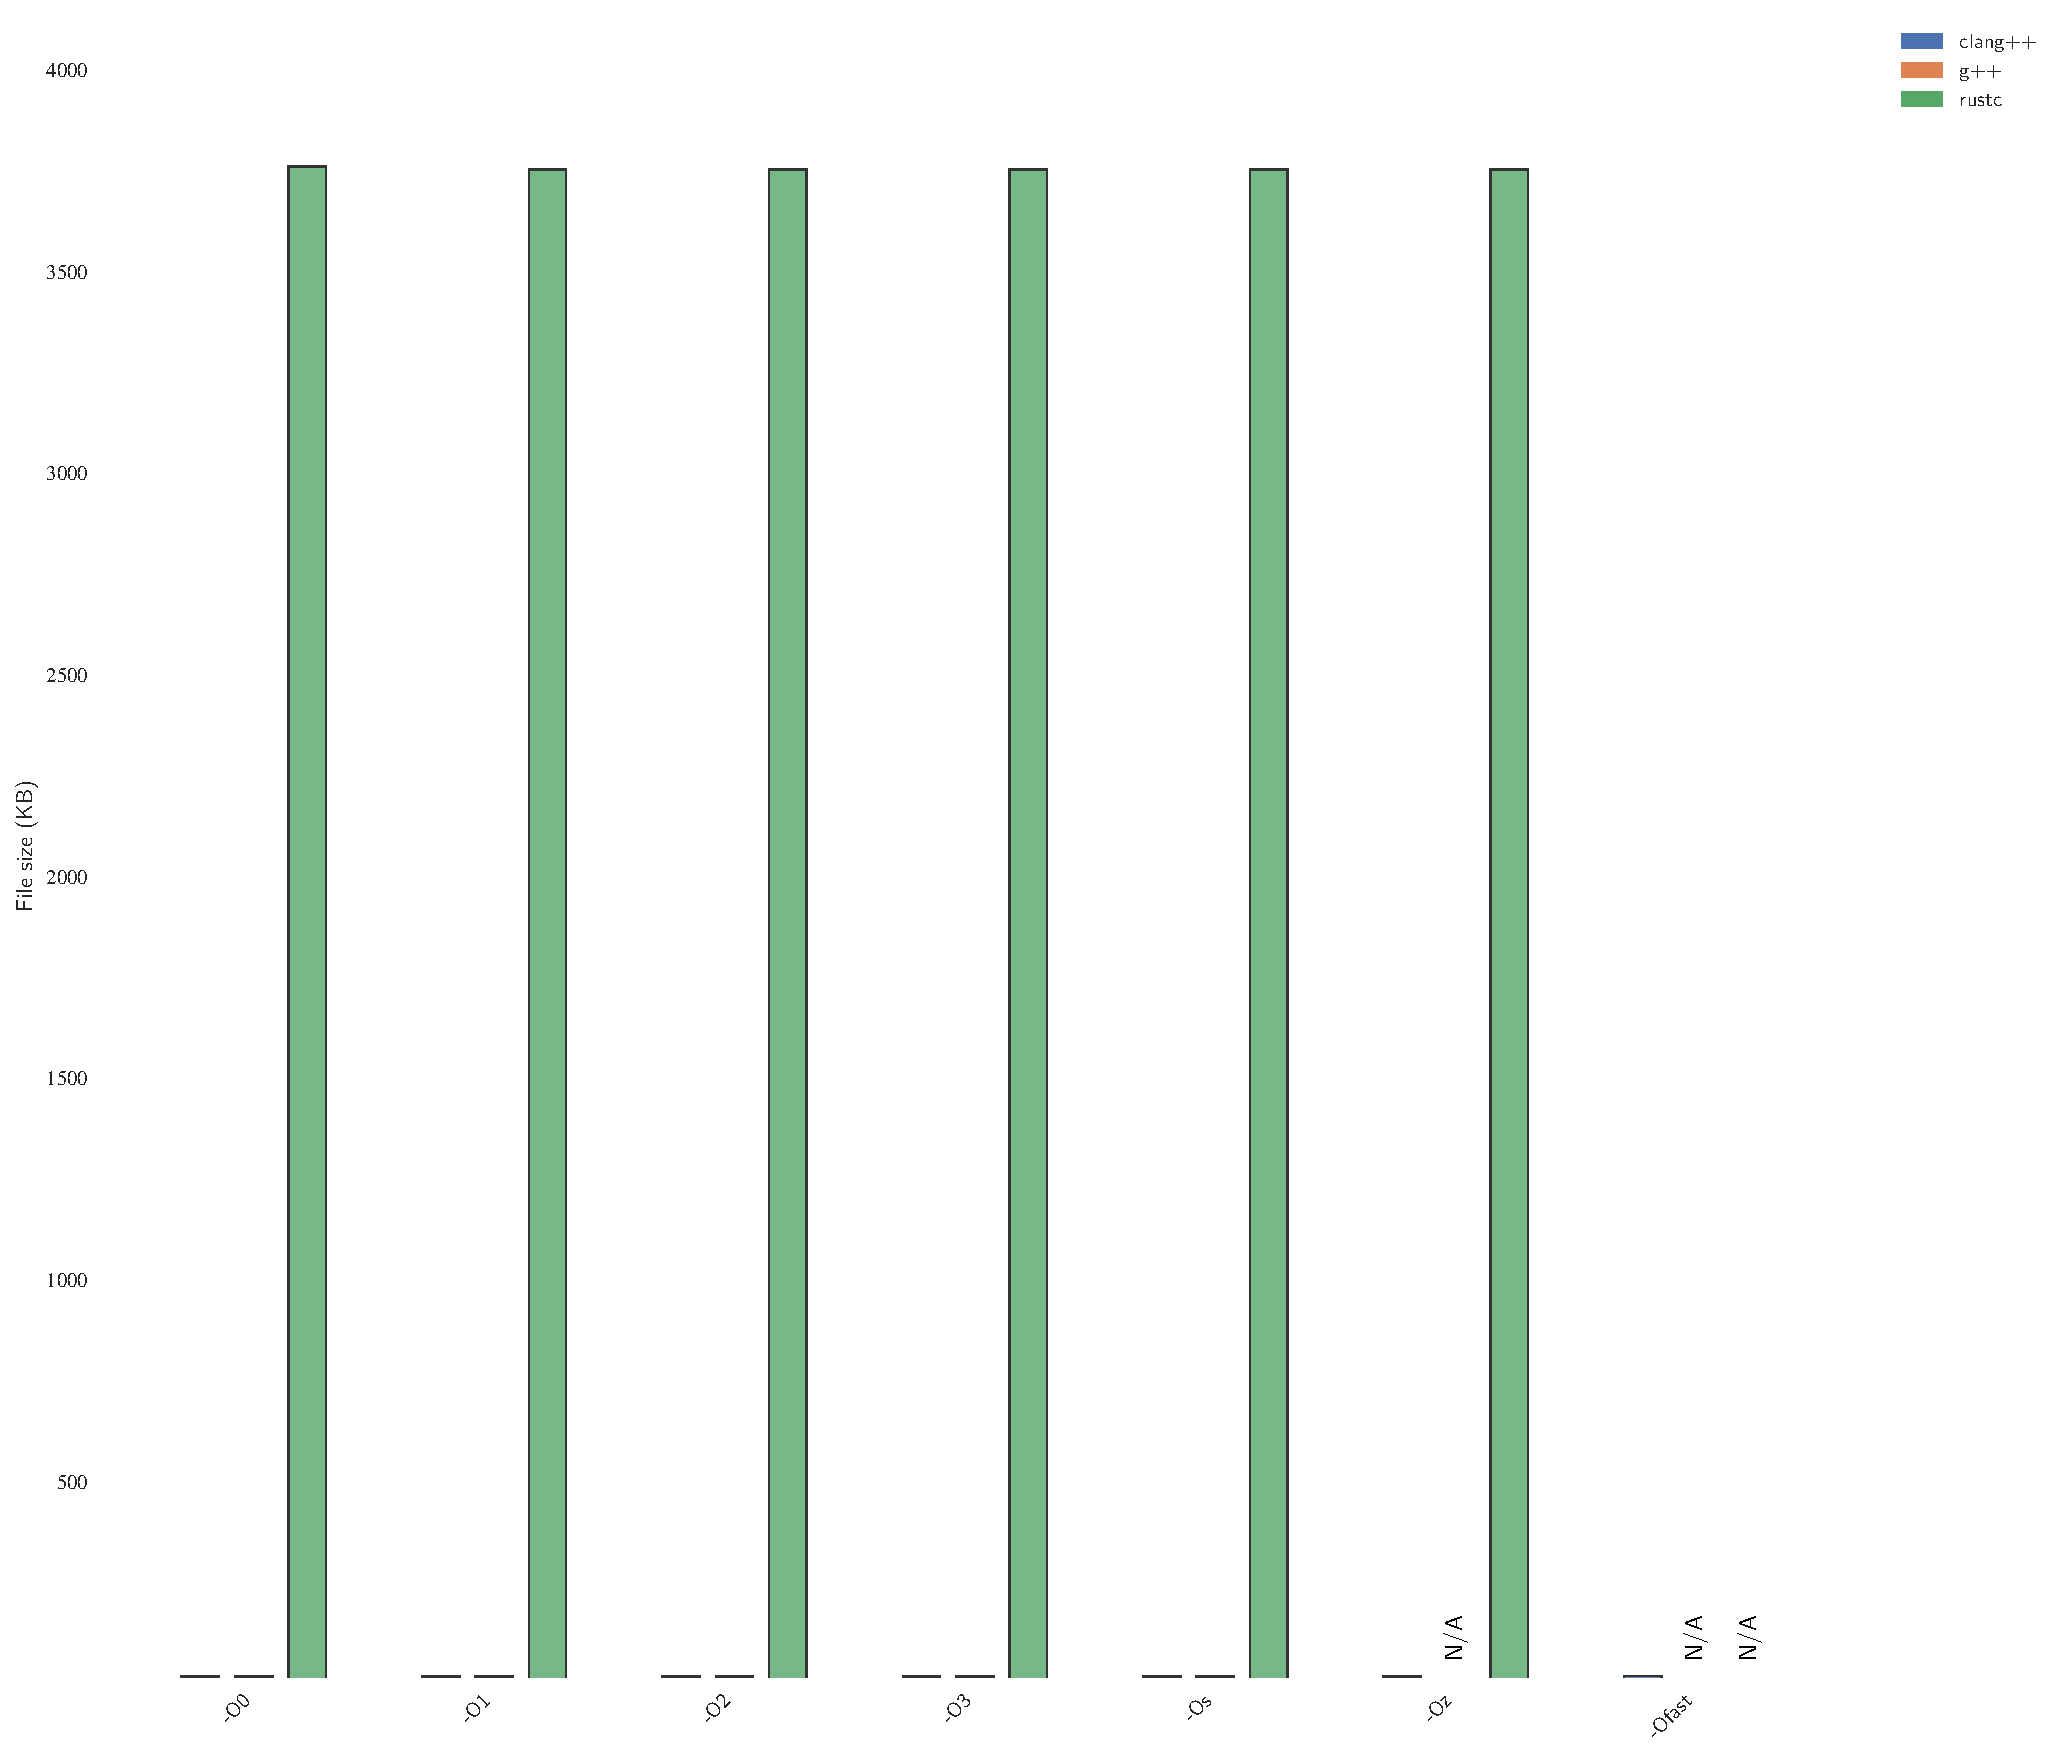
\includegraphics[width=\linewidth]{Gráficas/Gráficas_por_medida_seguridad/stack-protection/strong/File_size_KB.pdf}
      \label{fig:Gráficas_gráficas_por_medida_seguridad_stack_protection_strong_file_size_kb}
    }
  \end{minipage}
  \hfill
  \begin{minipage}{0.48\textwidth}
    \centering
    \subfloat[Funciones fortificadas (\%)]{
      \includegraphics[width=\linewidth]{Gráficas/Gráficas_por_medida_seguridad/stack-protection/strong/Fortified_Functions.pdf}
      \label{fig:Gráficas_gráficas_por_medida_seguridad_stack_protection_strong_fortified_functions}
    }
  \end{minipage}


  \vspace{1cm}

  \begin{minipage}{0.48\textwidth}
    \centering
    \subfloat[Uso de memoria (KB)]{
      
\includegraphics[width=\linewidth]{Gráficas/Gráficas_por_medida_seguridad/stack-protection/strong/Memory_usage_KB.pdf}
      \label{fig:Gráficas_gráficas_por_medida_seguridad_stack_protection_strong_memory_usage_kb}
    }
  \end{minipage}
  \hfill
  \begin{minipage}{0.48\textwidth}
    \centering
    \subfloat[Tiempo (ms)]{
      
\includegraphics[width=\linewidth]{Gráficas/Gráficas_por_medida_seguridad/stack-protection/strong/Time_ms.pdf}
      \label{fig:Gráficas_gráficas_por_medida_seguridad_stack_protection_strong_time_ms}
    }
  \end{minipage}

\end{figure}
\newpage

\section*{Gráficas Por Optimización Porcentual}

% === Gráficas_por_optimización_porcentual/-O0 ===
\subsection*{-O0}
\begin{figure}[htbp]
  \centering
  \caption{Resultados de compilación con optimización \texttt{-O0}}
  \vspace{0.5cm}

  \begin{minipage}{0.48\textwidth}
    \centering
    \subfloat[Tamaño del archivo (KB)]{
      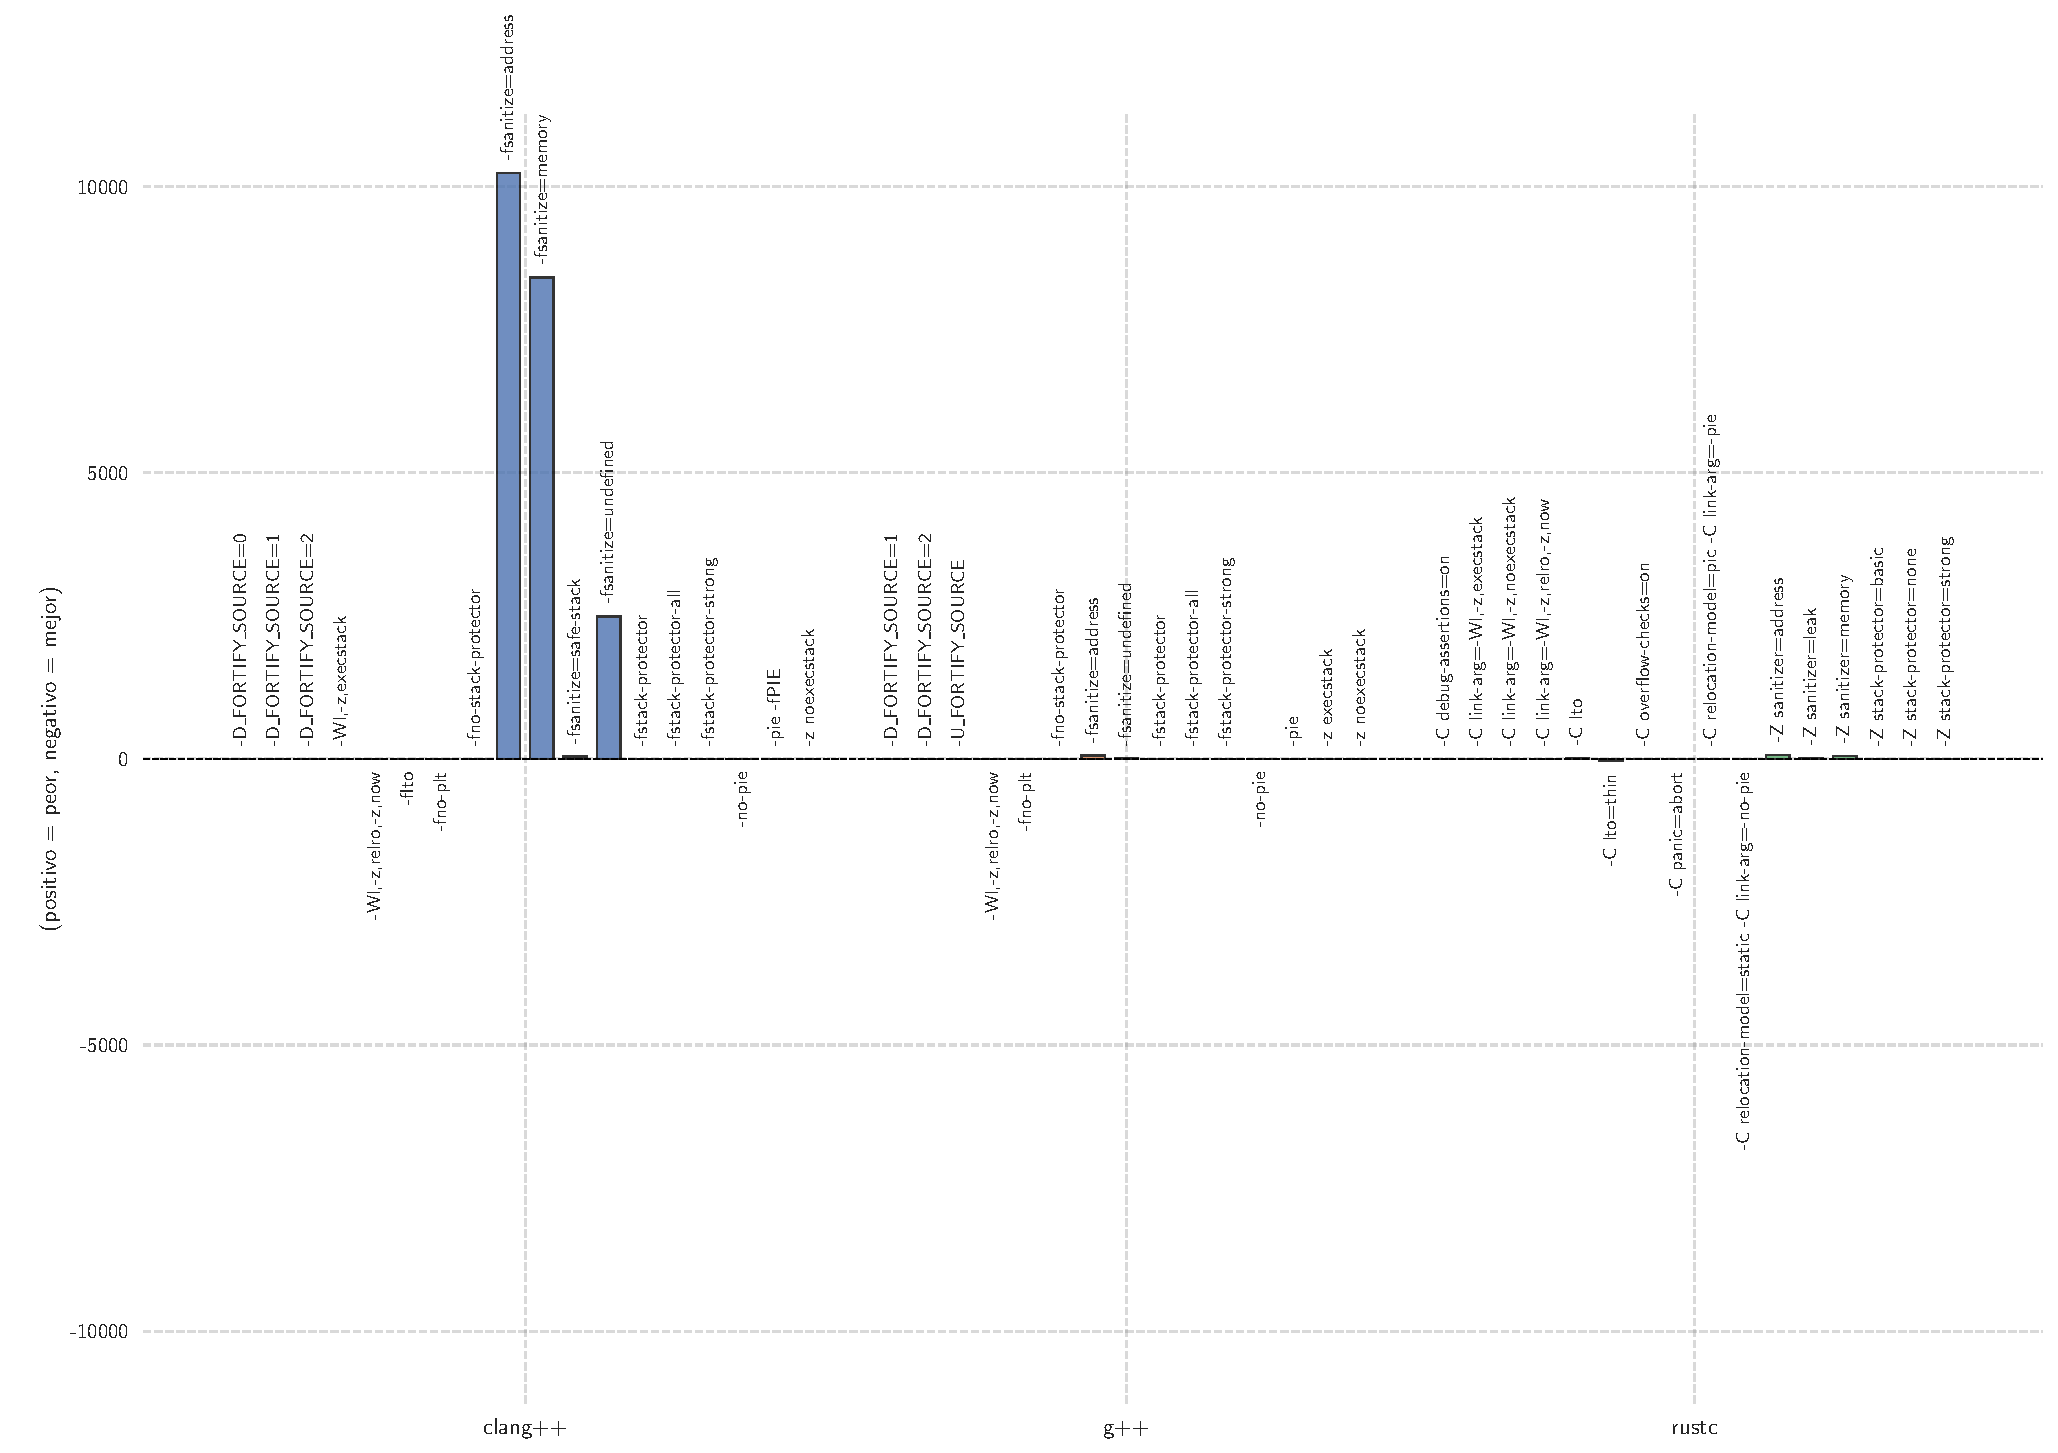
\includegraphics[width=\linewidth]{Gráficas/Gráficas_por_optimización_porcentual/-O0/File_size_KB.pdf}
      \label{fig:Gráficas_gráficas_por_optimización_porcentual__o0_file_size_kb}
    }
  \end{minipage}
  \hfill
  \begin{minipage}{0.48\textwidth}
    \centering
    \subfloat[Funciones fortificadas (\%)]{
      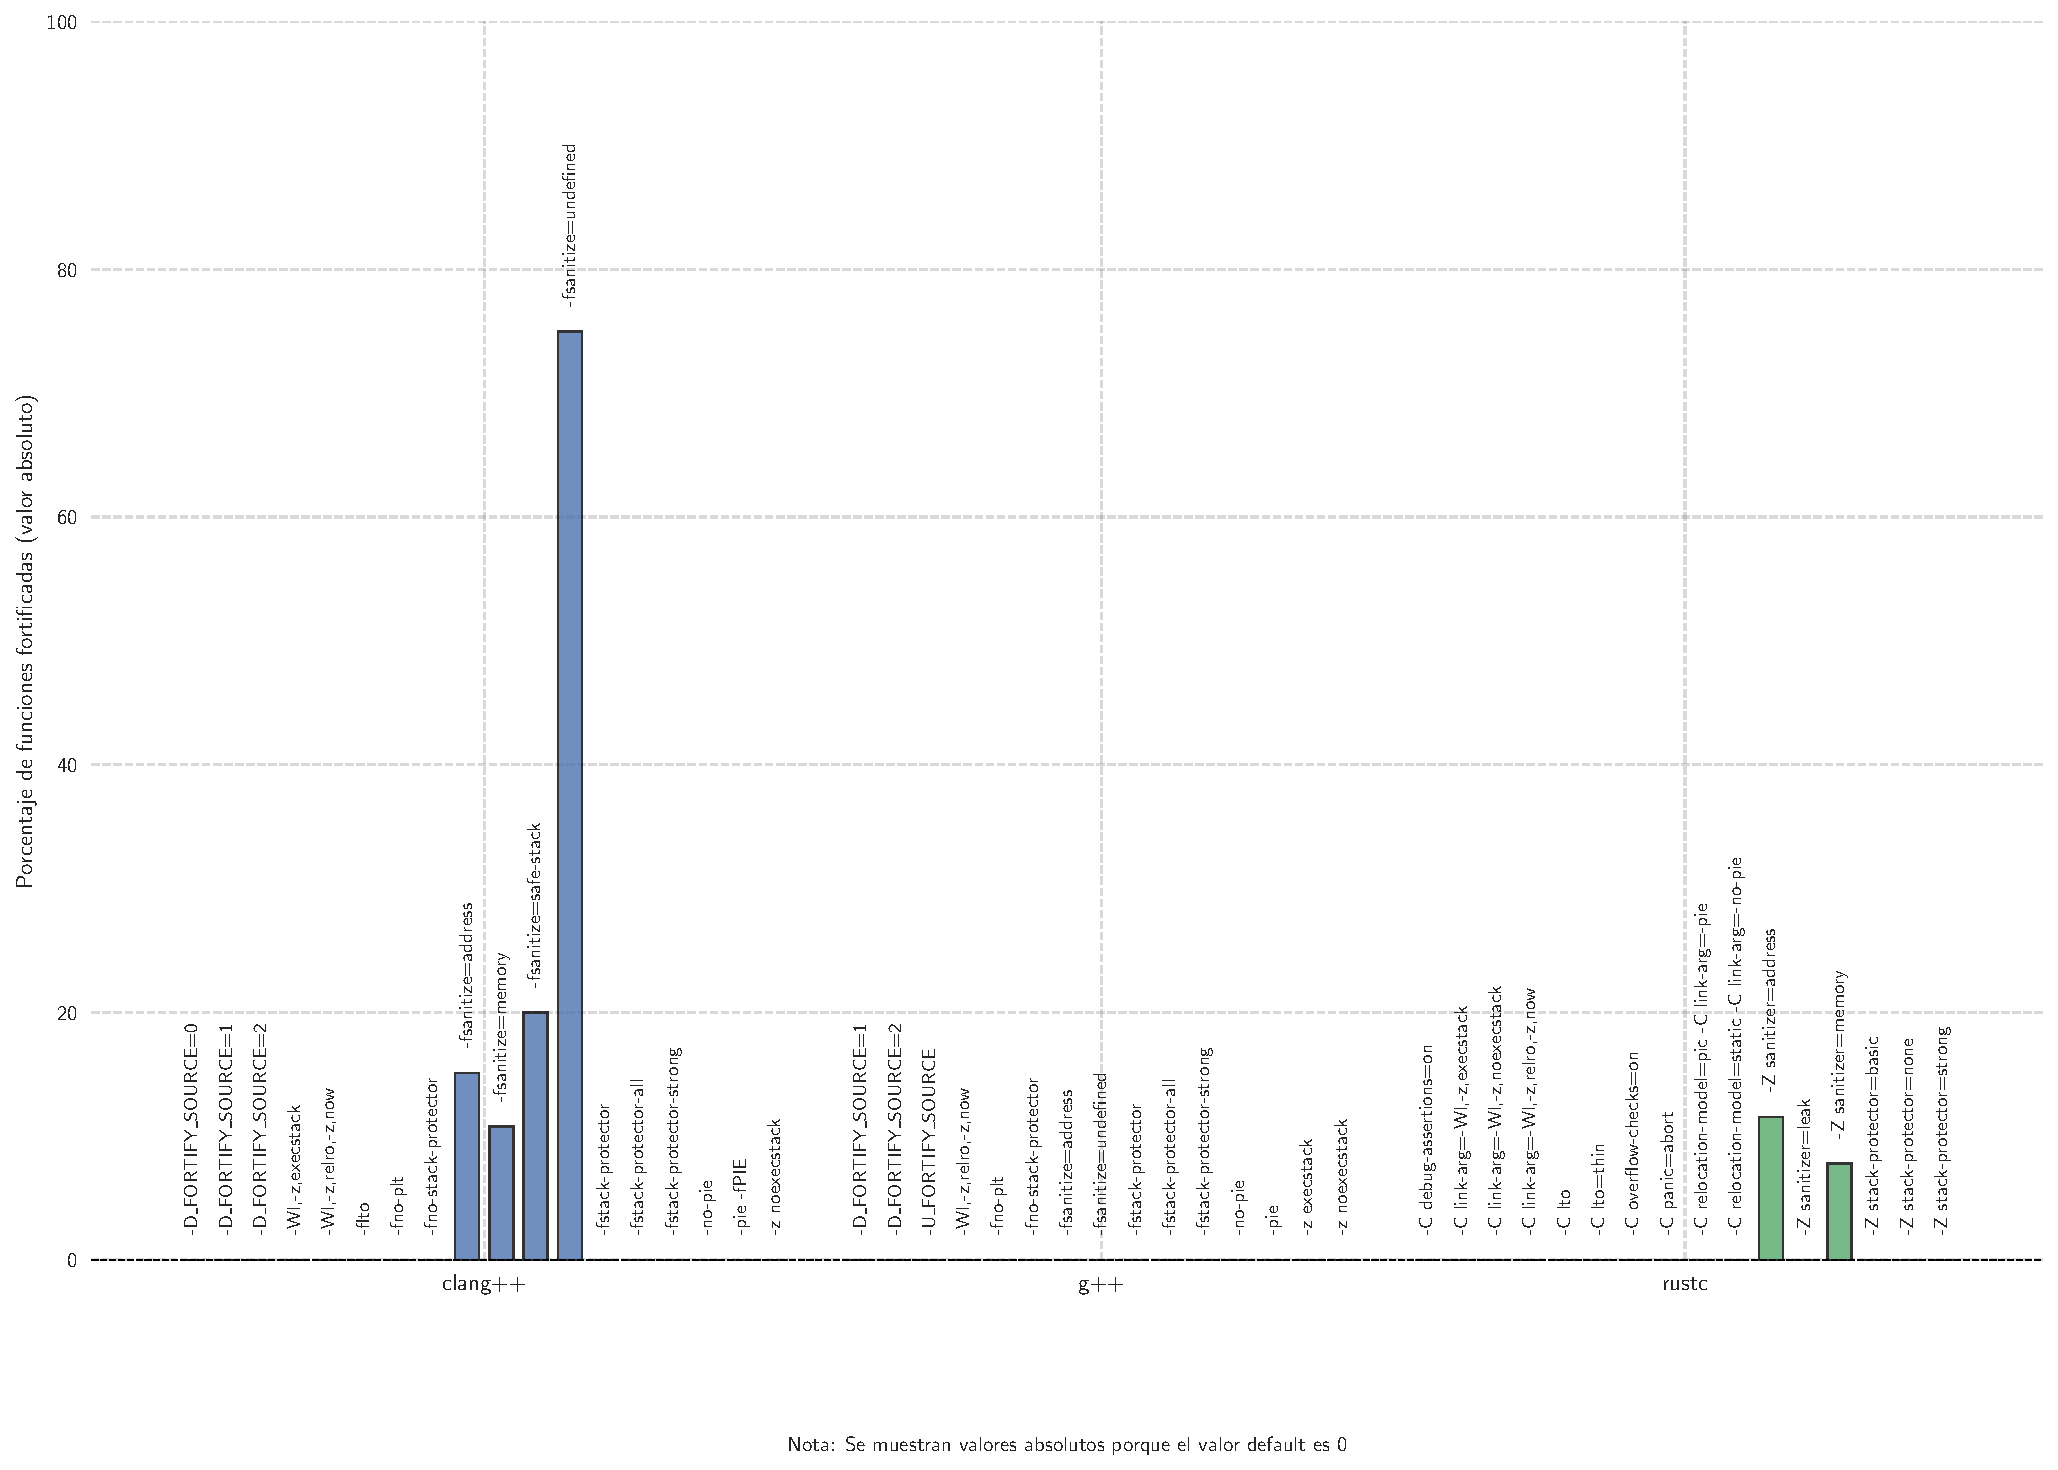
\includegraphics[width=\linewidth]{Gráficas/Gráficas_por_optimización_porcentual/-O0/Fortified_Functions.pdf}
      \label{fig:Gráficas_gráficas_por_optimización_porcentual__o0_fortified_functions}
    }
  \end{minipage}


  \vspace{1cm}

  \begin{minipage}{0.48\textwidth}
    \centering
    \subfloat[Uso de memoria (KB)]{
      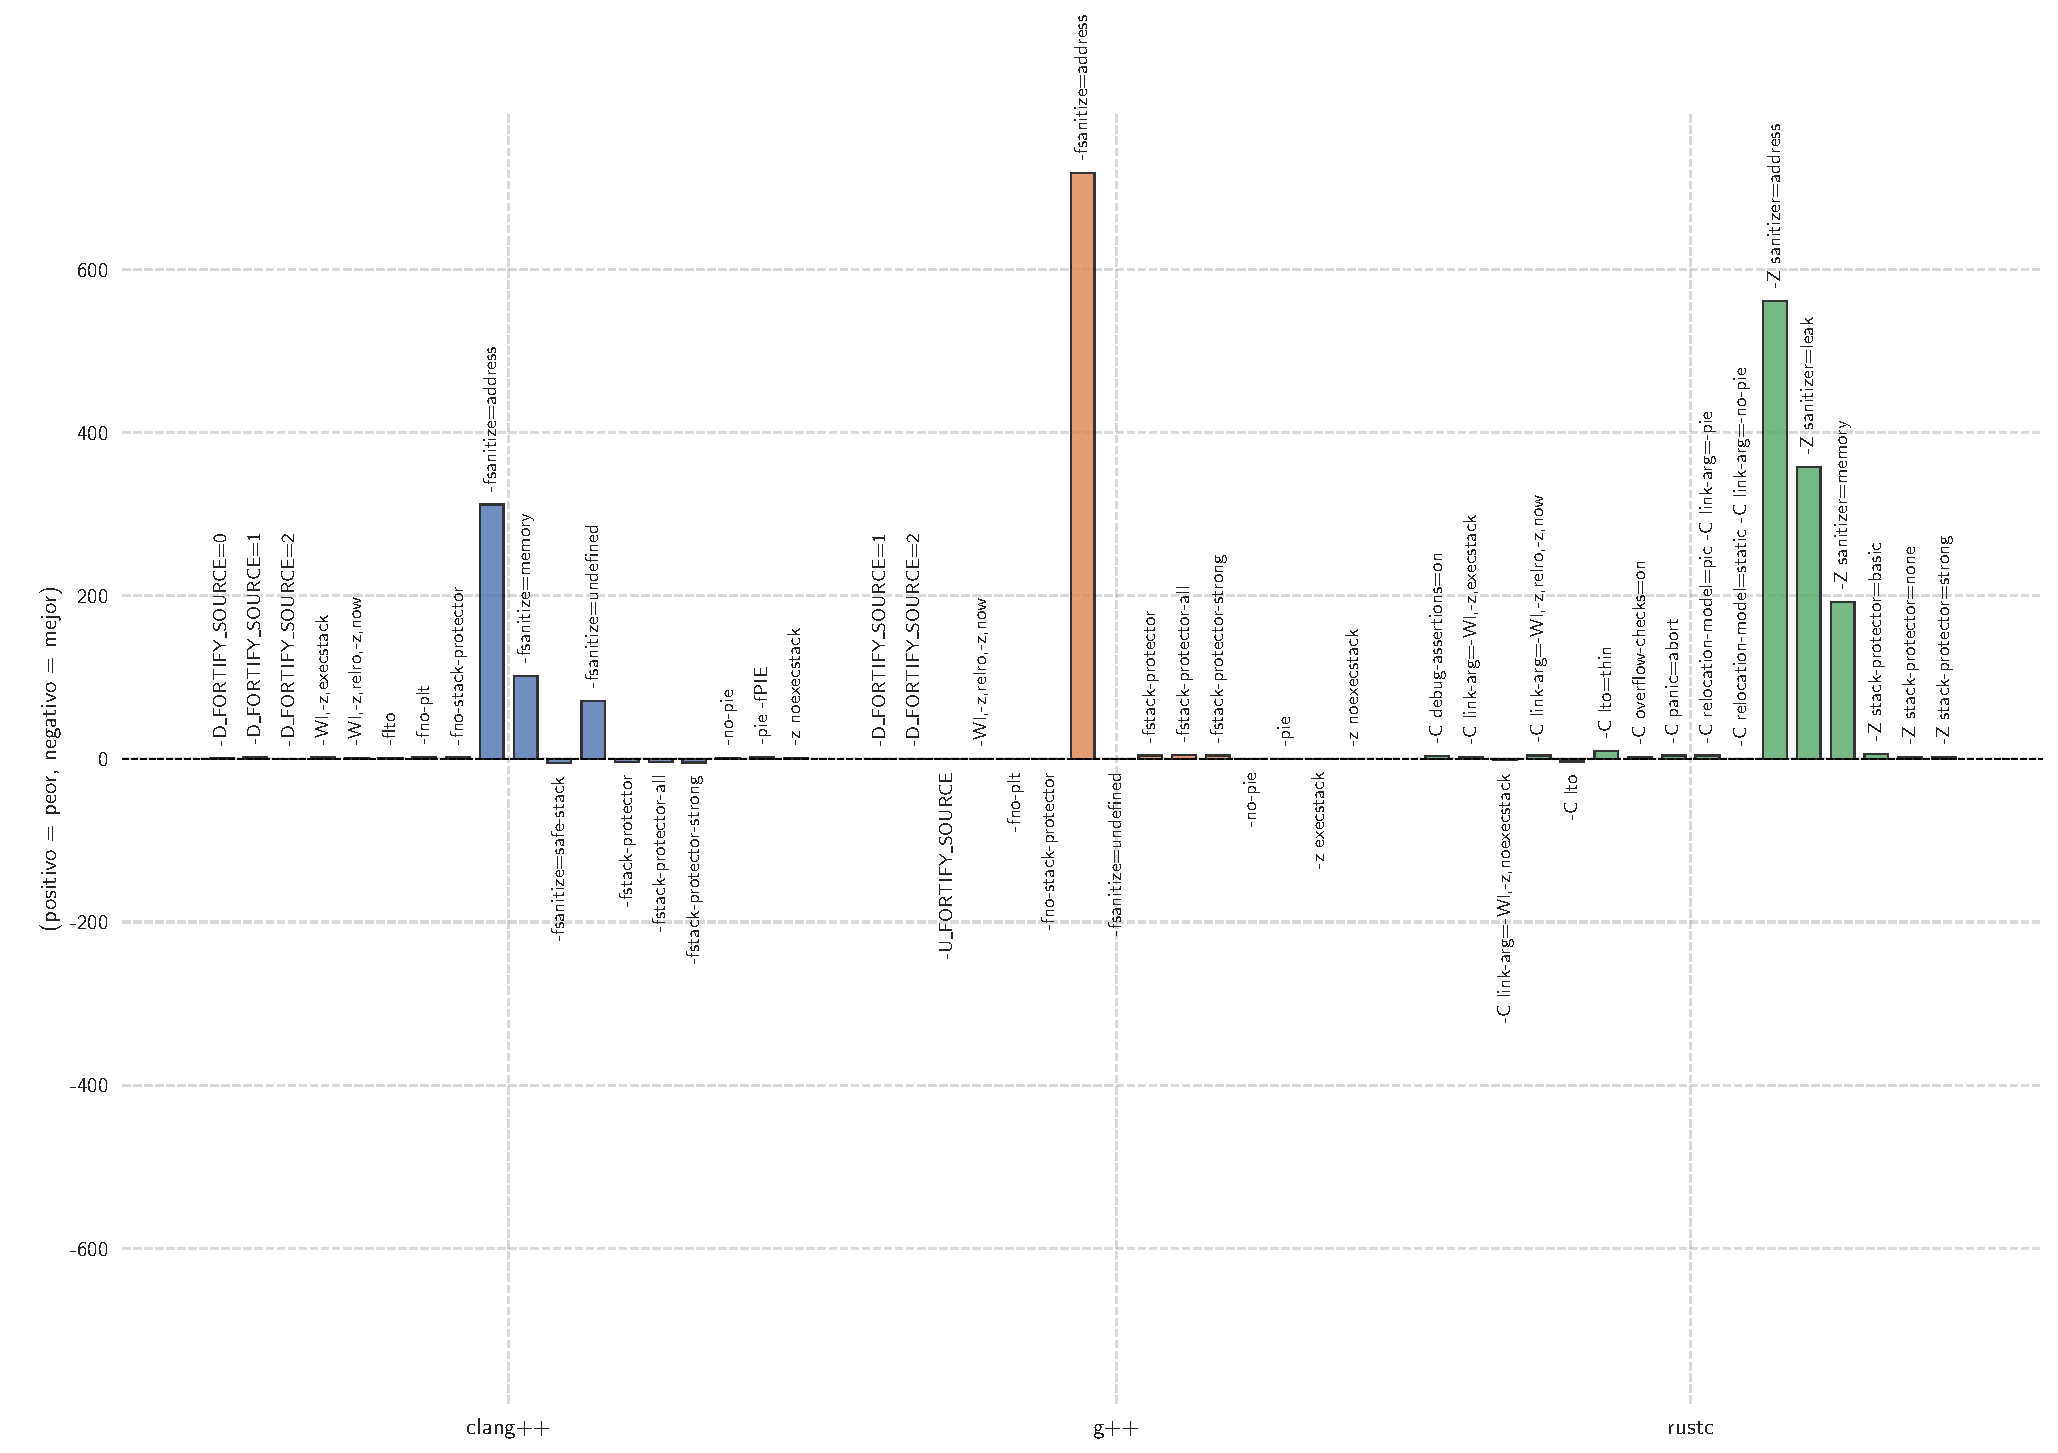
\includegraphics[width=\linewidth]{Gráficas/Gráficas_por_optimización_porcentual/-O0/Memory_usage_KB.pdf}
      \label{fig:Gráficas_gráficas_por_optimización_porcentual__o0_memory_usage_kb}
    }
  \end{minipage}
  \hfill
  \begin{minipage}{0.48\textwidth}
    \centering
    \subfloat[Tiempo (ms)]{
      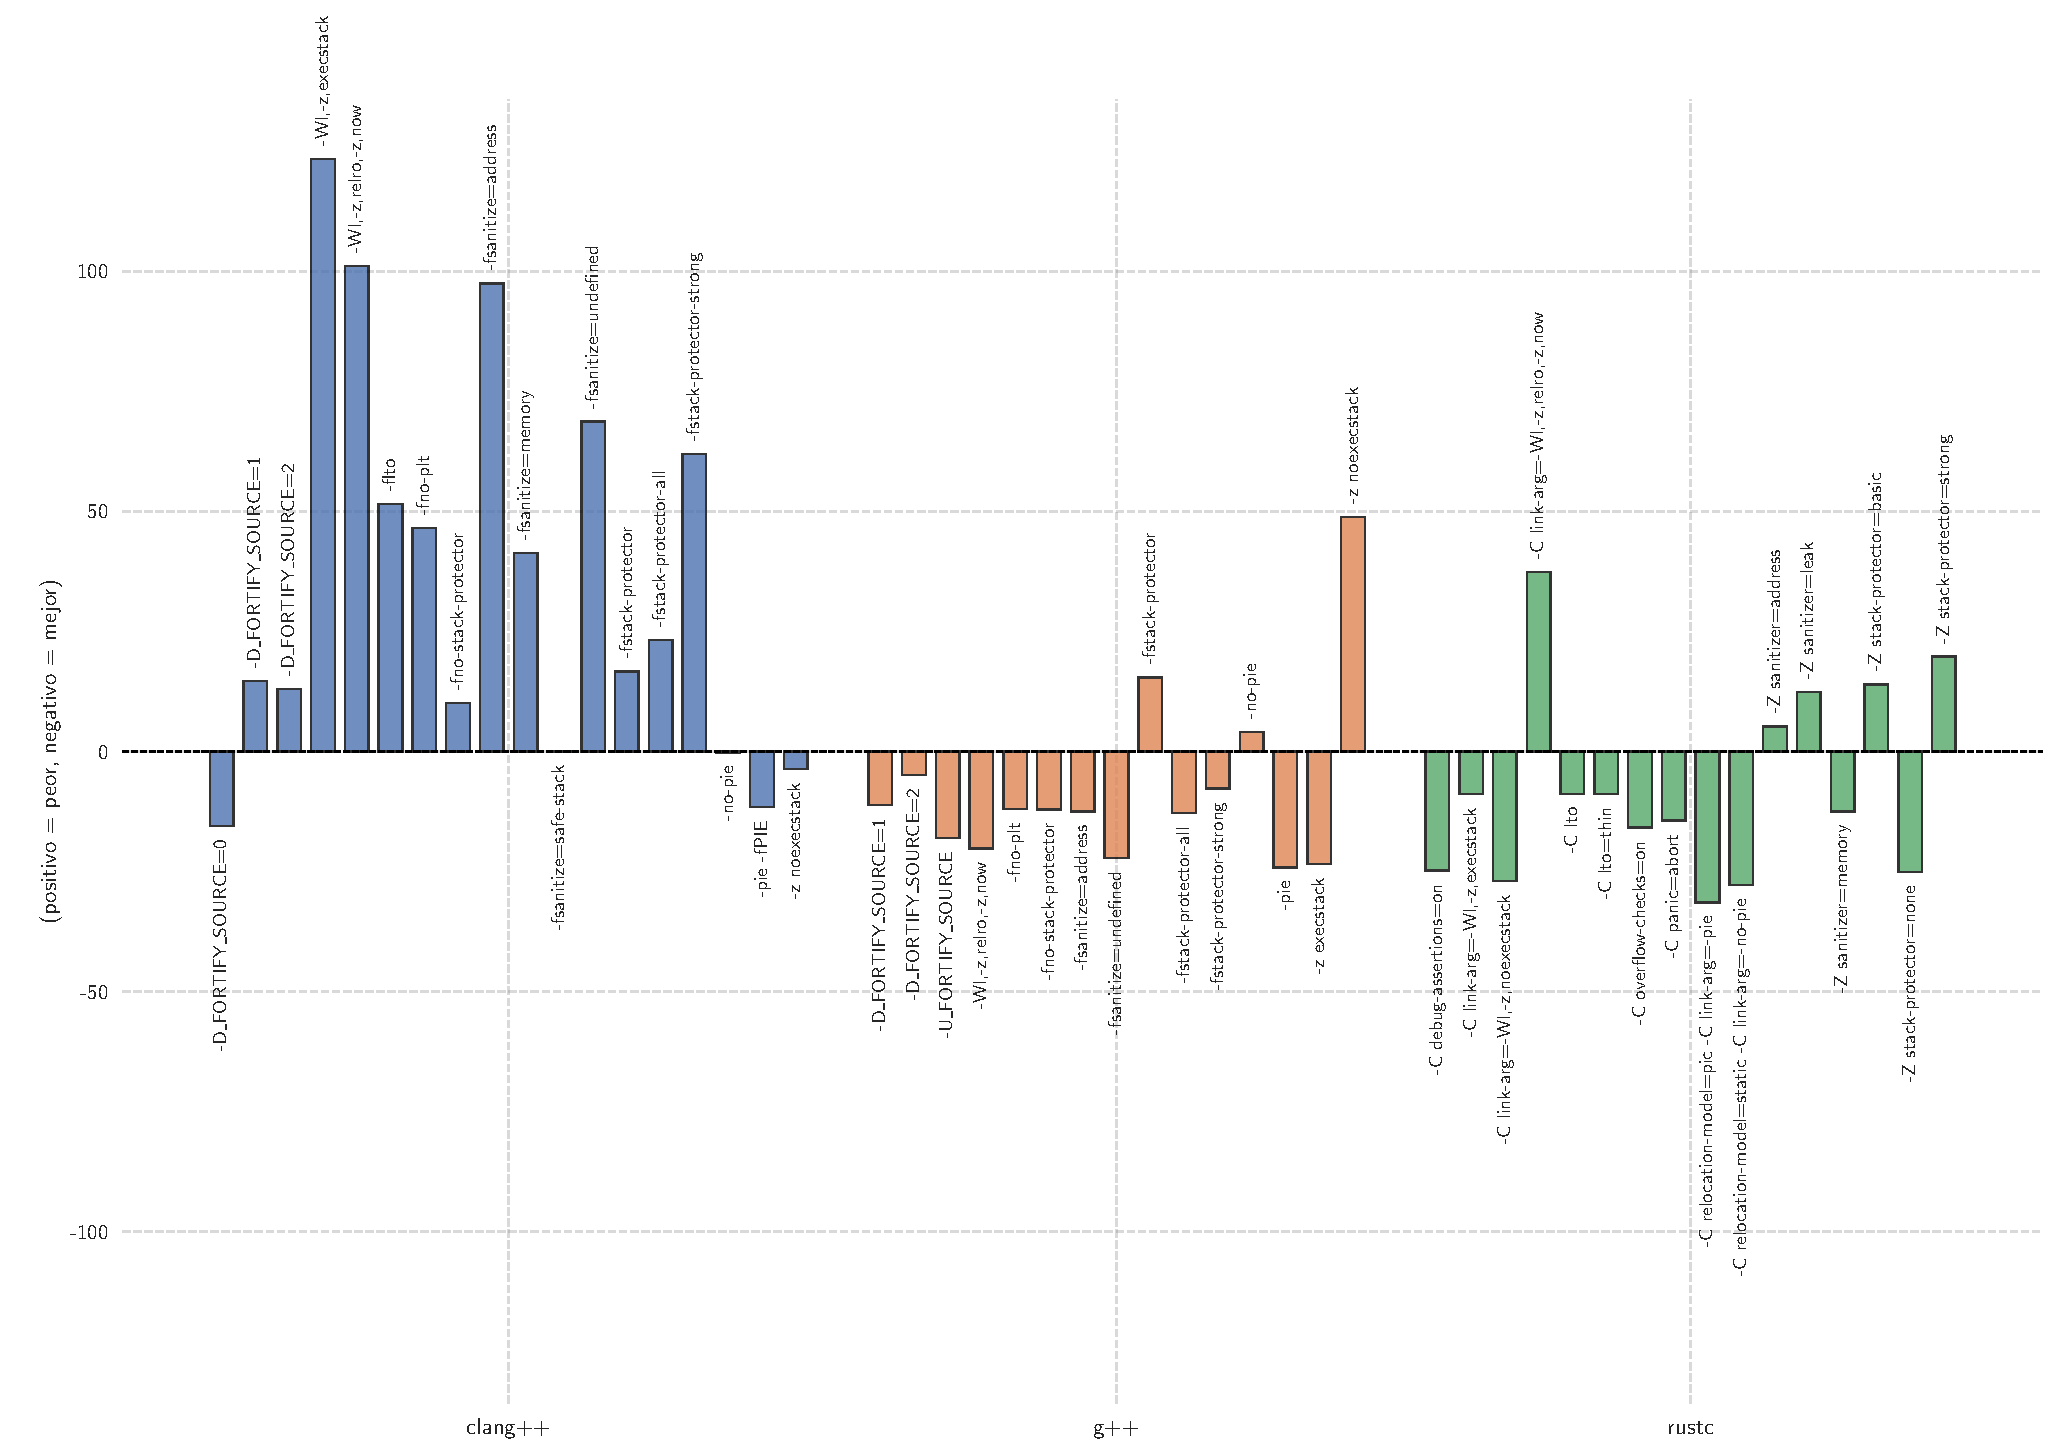
\includegraphics[width=\linewidth]{Gráficas/Gráficas_por_optimización_porcentual/-O0/Time_ms.pdf}
      \label{fig:Gráficas_gráficas_por_optimización_porcentual__o0_time_ms}
    }
  \end{minipage}

\end{figure}
\newpage

% === Gráficas_por_optimización_porcentual/-O1 ===
\subsection*{-O1}
\begin{figure}[htbp]
  \centering
  \caption{Resultados de compilación con optimización \texttt{-O1}}
  \vspace{0.5cm}

  \begin{minipage}{0.48\textwidth}
    \centering
    \subfloat[Tamaño del archivo (KB)]{
      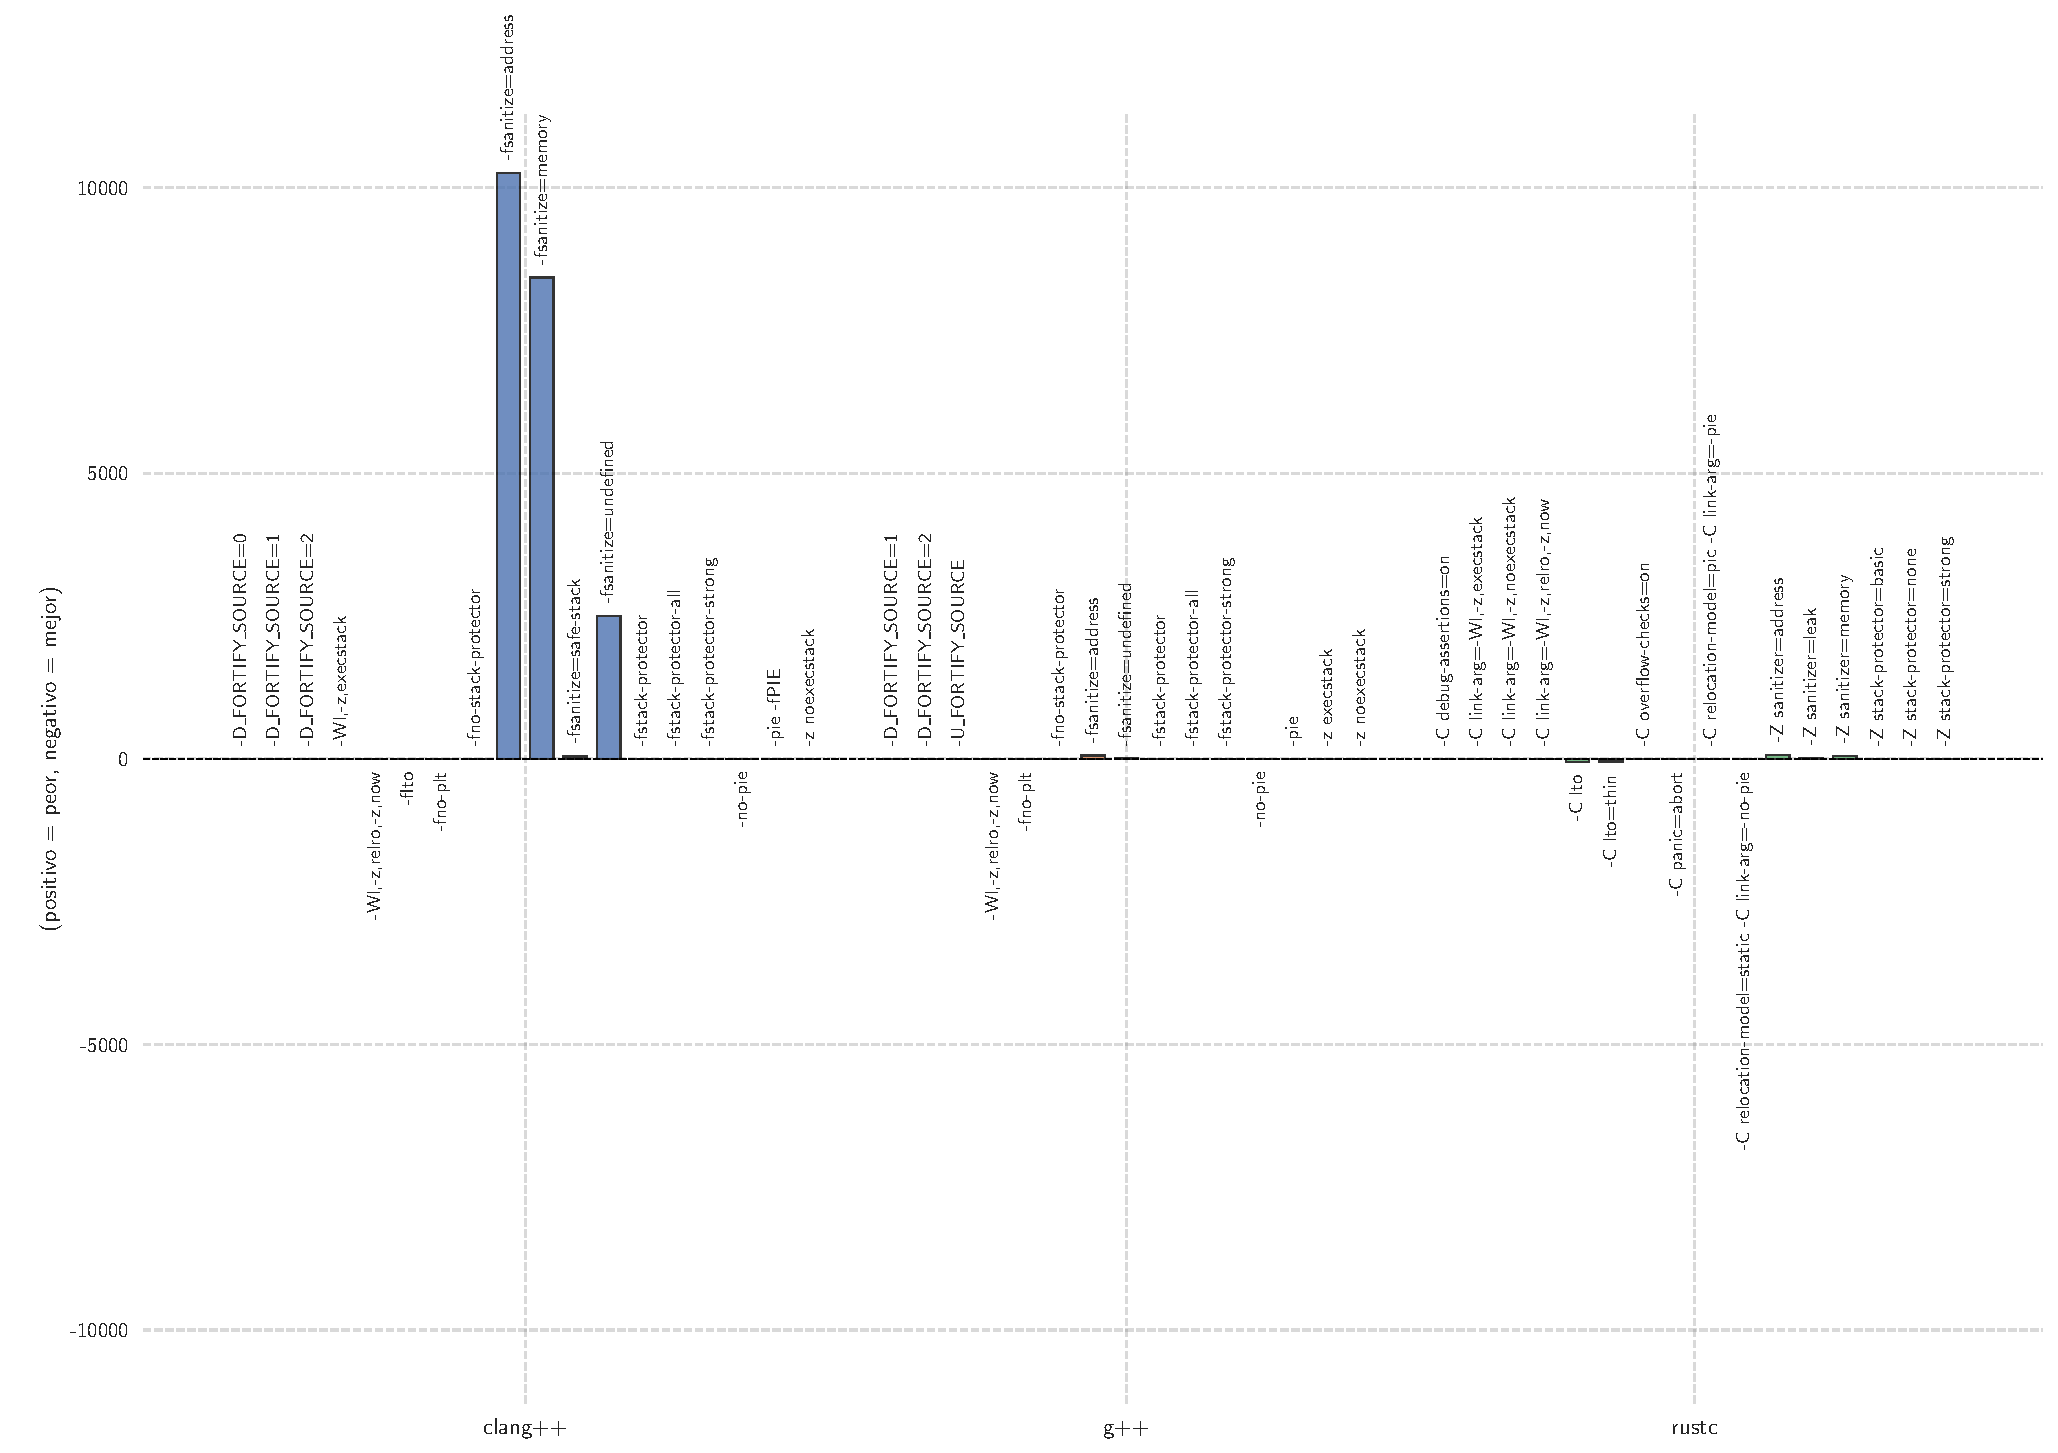
\includegraphics[width=\linewidth]{Gráficas/Gráficas_por_optimización_porcentual/-O1/File_size_KB.pdf}
      \label{fig:Gráficas_gráficas_por_optimización_porcentual__o1_file_size_kb}
    }
  \end{minipage}
  \hfill
  \begin{minipage}{0.48\textwidth}
    \centering
    \subfloat[Funciones fortificadas (\%)]{
      \includegraphics[width=\linewidth]{Gráficas/Gráficas_por_optimización_porcentual/-O1/Fortified_Functions.pdf}
      \label{fig:Gráficas_gráficas_por_optimización_porcentual__o1_fortified_functions}
    }
  \end{minipage}


  \vspace{1cm}

  \begin{minipage}{0.48\textwidth}
    \centering
    \subfloat[Uso de memoria (KB)]{
      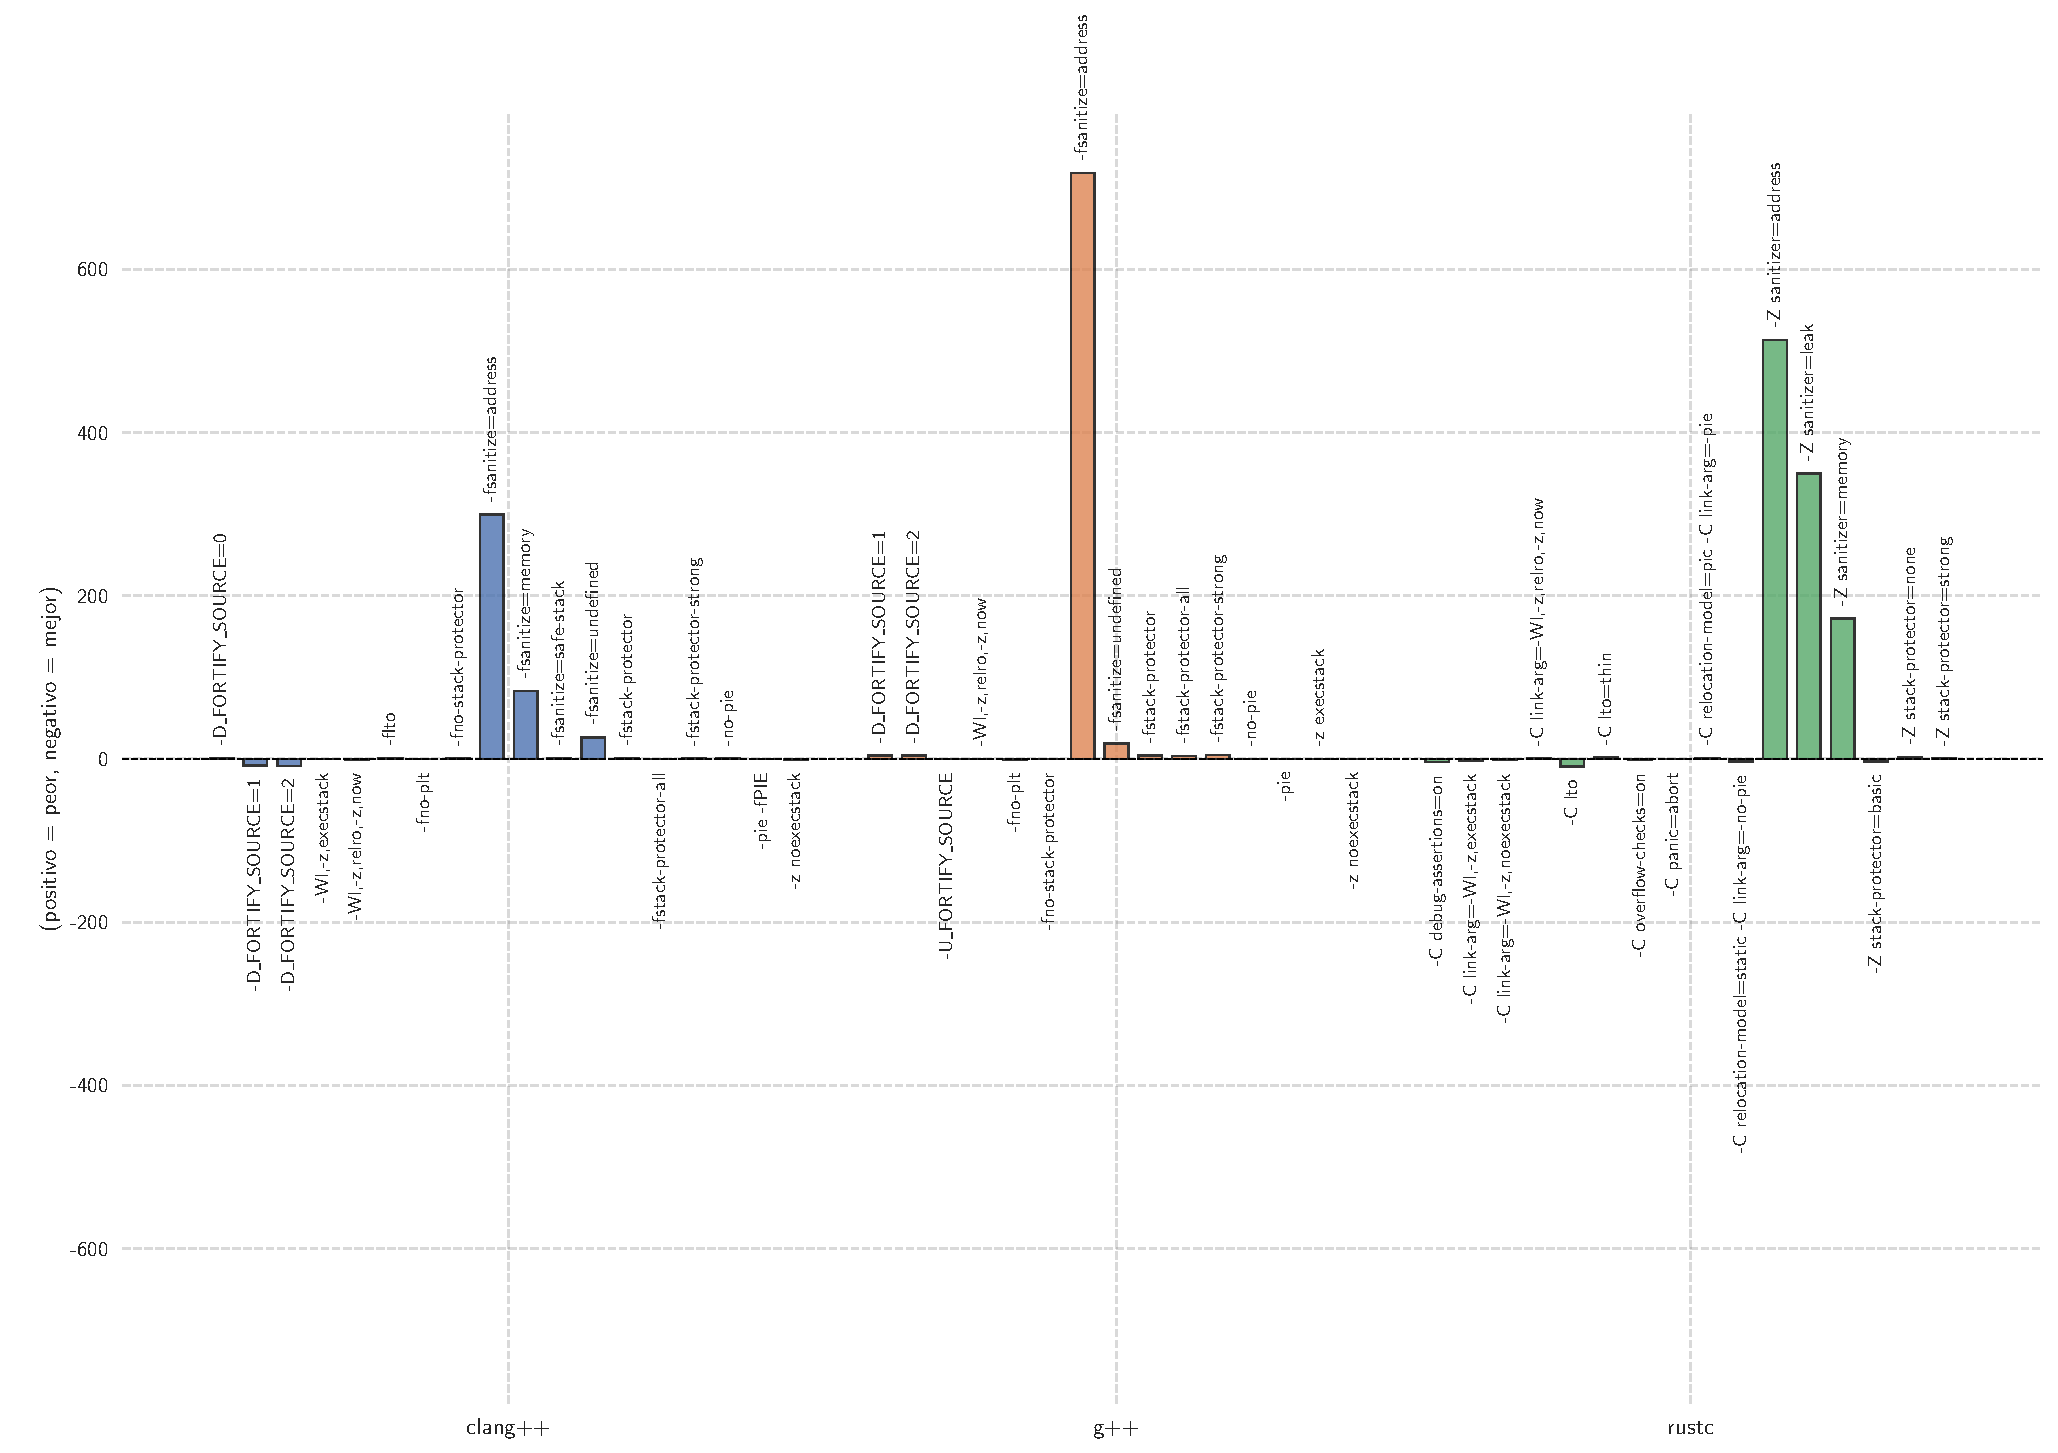
\includegraphics[width=\linewidth]{Gráficas/Gráficas_por_optimización_porcentual/-O1/Memory_usage_KB.pdf}
      \label{fig:Gráficas_gráficas_por_optimización_porcentual__o1_memory_usage_kb}
    }
  \end{minipage}
  \hfill
  \begin{minipage}{0.48\textwidth}
    \centering
    \subfloat[Tiempo (ms)]{
      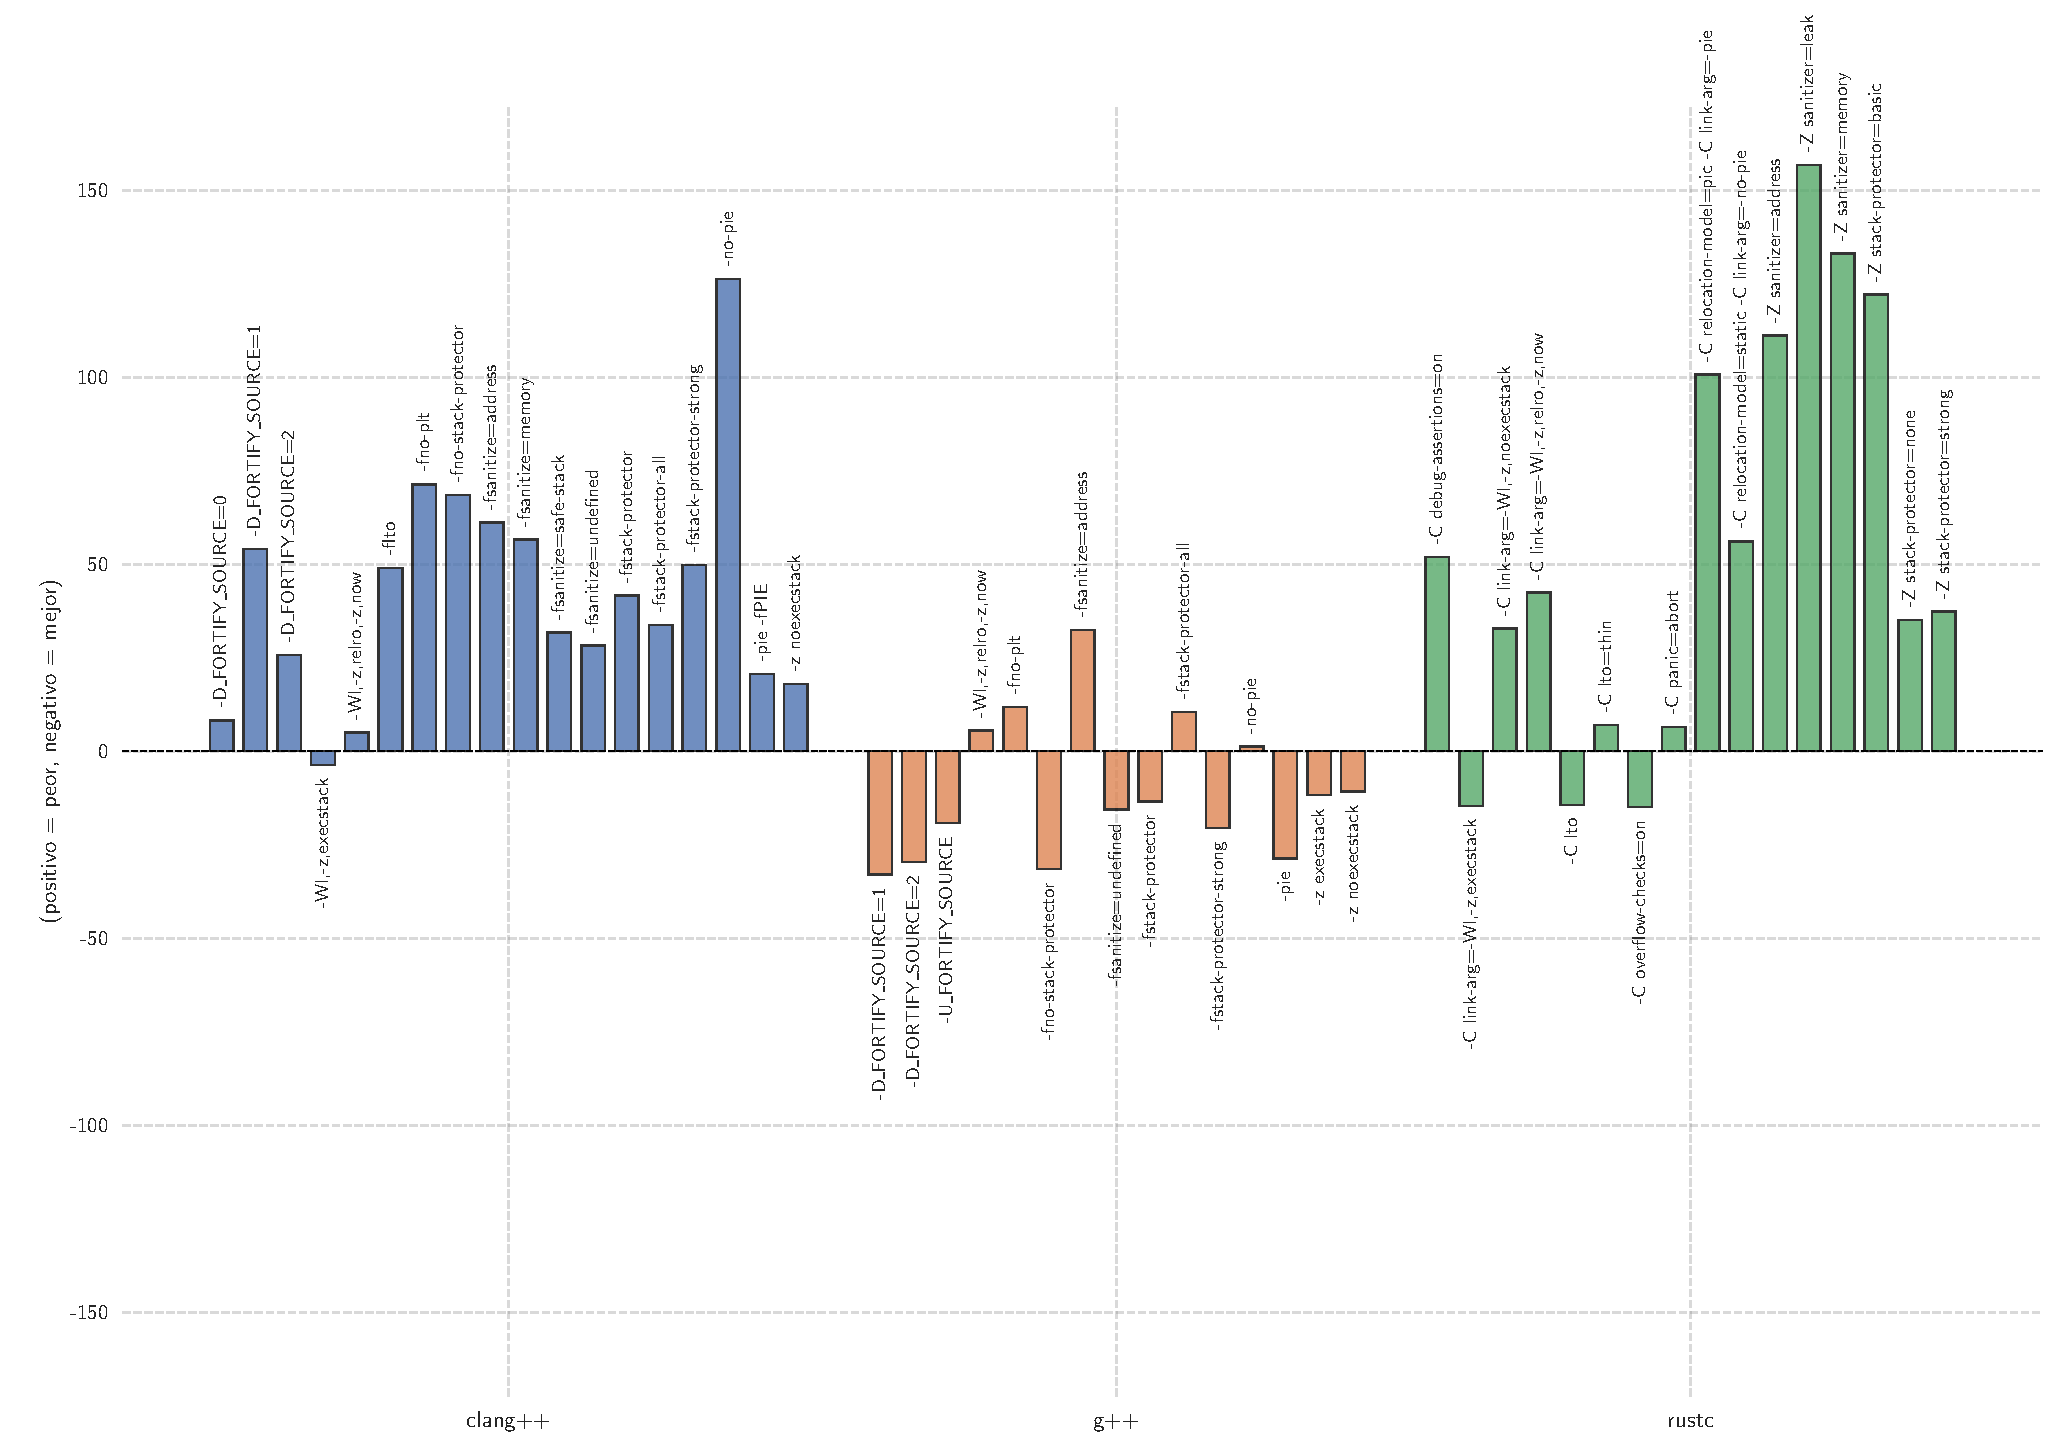
\includegraphics[width=\linewidth]{Gráficas/Gráficas_por_optimización_porcentual/-O1/Time_ms.pdf}
      \label{fig:Gráficas_gráficas_por_optimización_porcentual__o1_time_ms}
    }
  \end{minipage}

\end{figure}
\newpage

% === Gráficas_por_optimización_porcentual/-O2 ===
\subsection*{-O2}
\begin{figure}[htbp]
  \centering
  \caption{Resultados de compilación con optimización \texttt{-O2}}
  \vspace{0.5cm}

  \begin{minipage}{0.48\textwidth}
    \centering
    \subfloat[Tamaño del archivo (KB)]{
      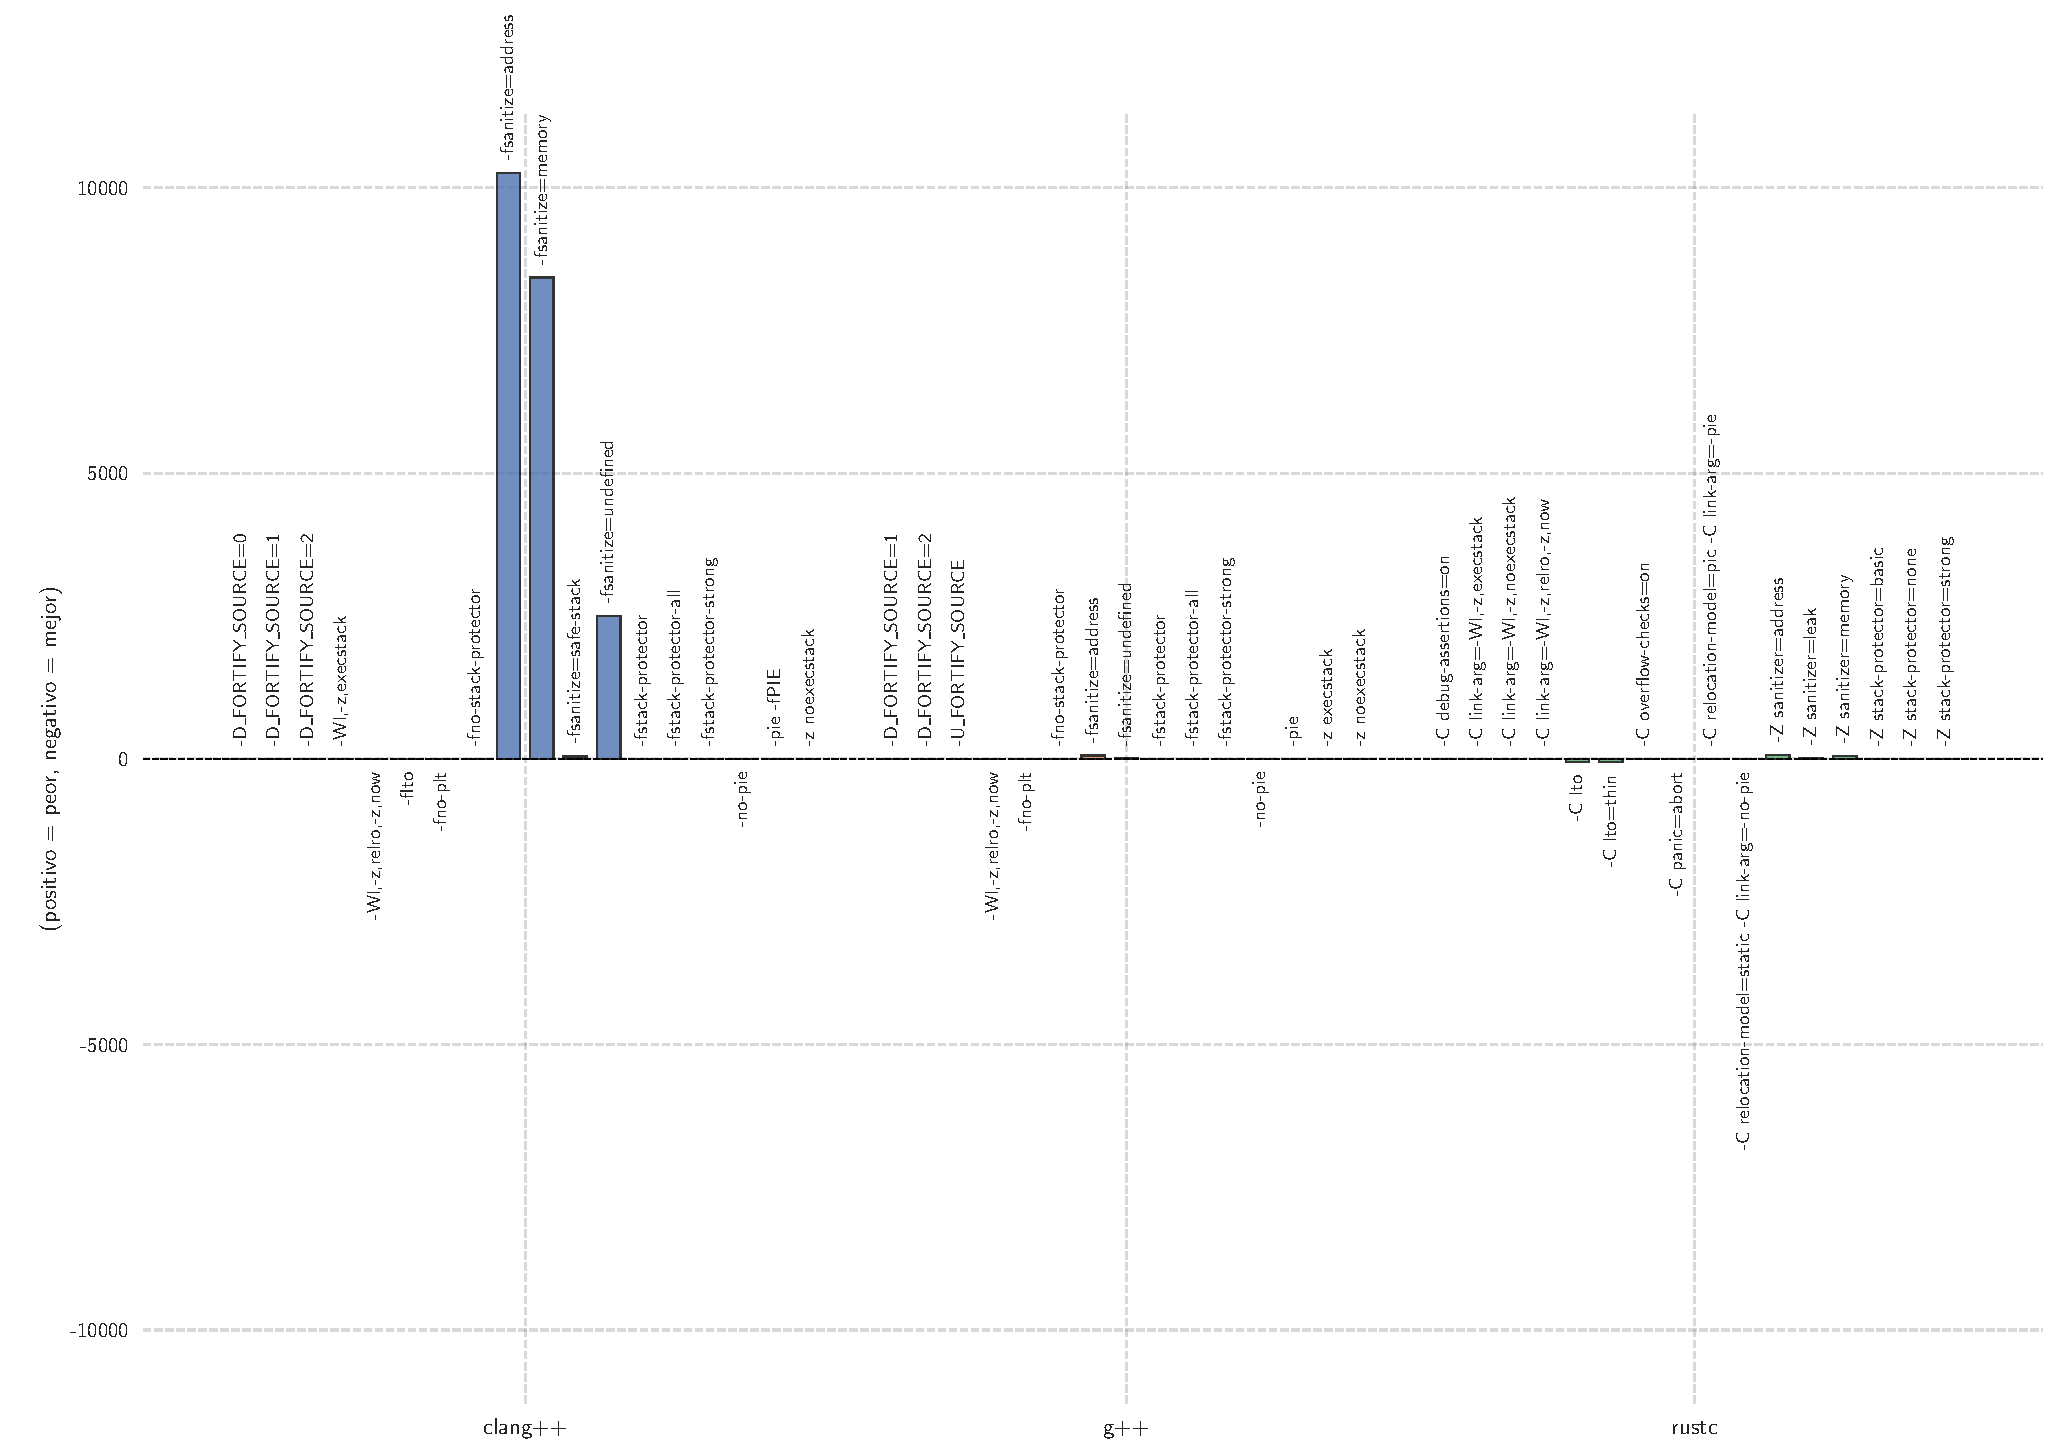
\includegraphics[width=\linewidth]{Gráficas/Gráficas_por_optimización_porcentual/-O2/File_size_KB.pdf}
      \label{fig:Gráficas_gráficas_por_optimización_porcentual__o2_file_size_kb}
    }
  \end{minipage}
  \hfill
  \begin{minipage}{0.48\textwidth}
    \centering
    \subfloat[Funciones fortificadas (\%)]{
      \includegraphics[width=\linewidth]{Gráficas/Gráficas_por_optimización_porcentual/-O2/Fortified_Functions.pdf}
      \label{fig:Gráficas_gráficas_por_optimización_porcentual__o2_fortified_functions}
    }
  \end{minipage}


  \vspace{1cm}

  \begin{minipage}{0.48\textwidth}
    \centering
    \subfloat[Uso de memoria (KB)]{
      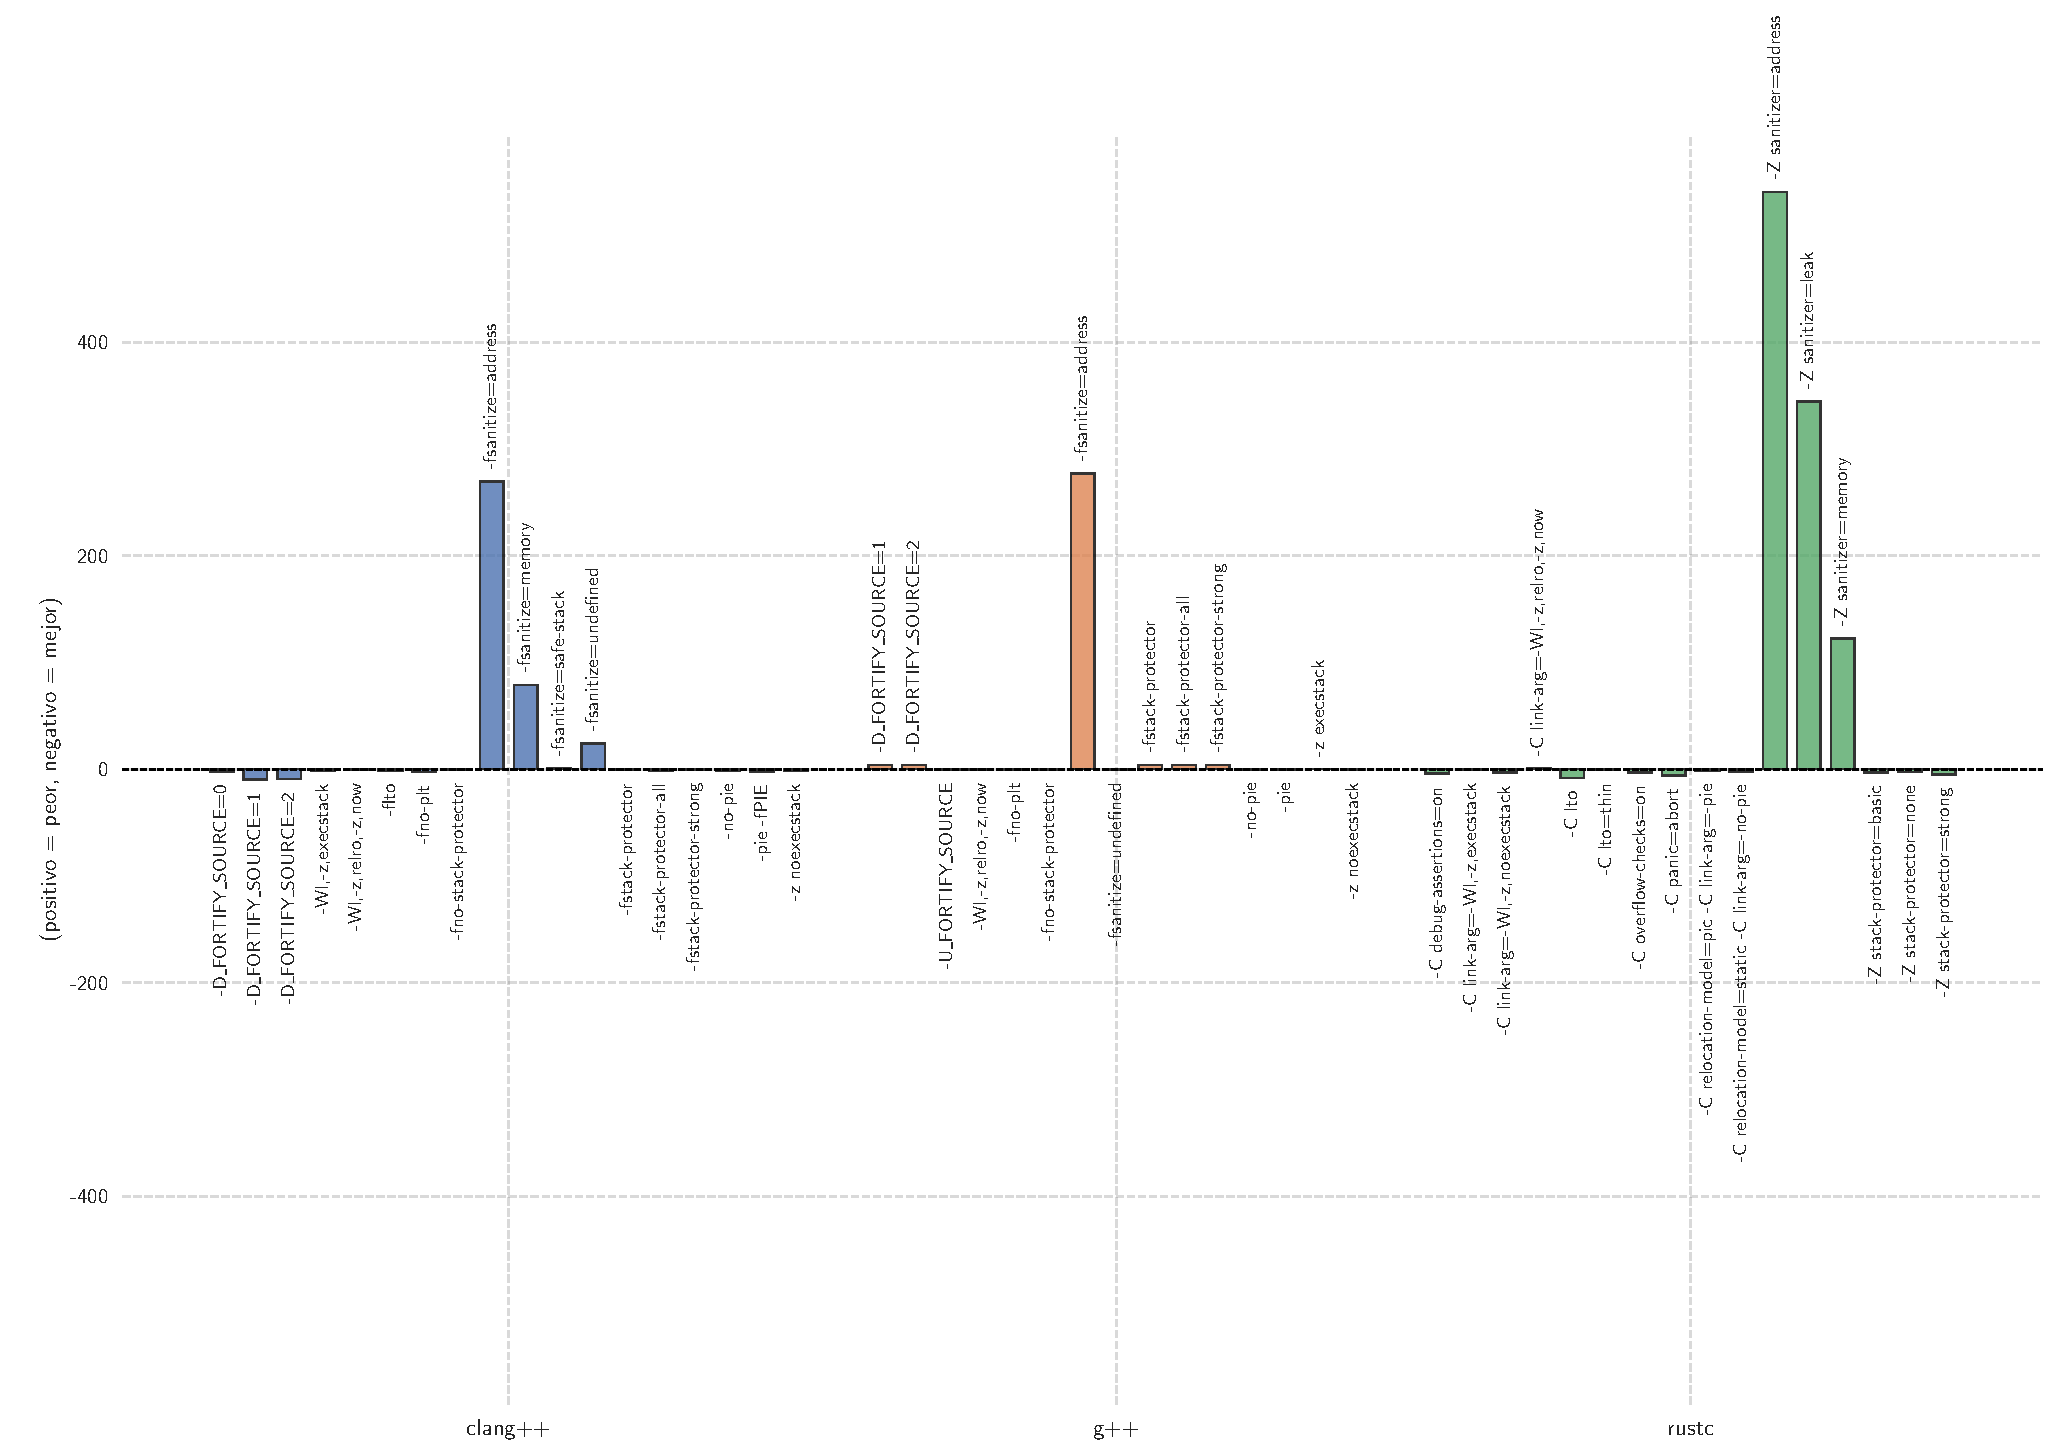
\includegraphics[width=\linewidth]{Gráficas/Gráficas_por_optimización_porcentual/-O2/Memory_usage_KB.pdf}
      \label{fig:Gráficas_gráficas_por_optimización_porcentual__o2_memory_usage_kb}
    }
  \end{minipage}
  \hfill
  \begin{minipage}{0.48\textwidth}
    \centering
    \subfloat[Tiempo (ms)]{
      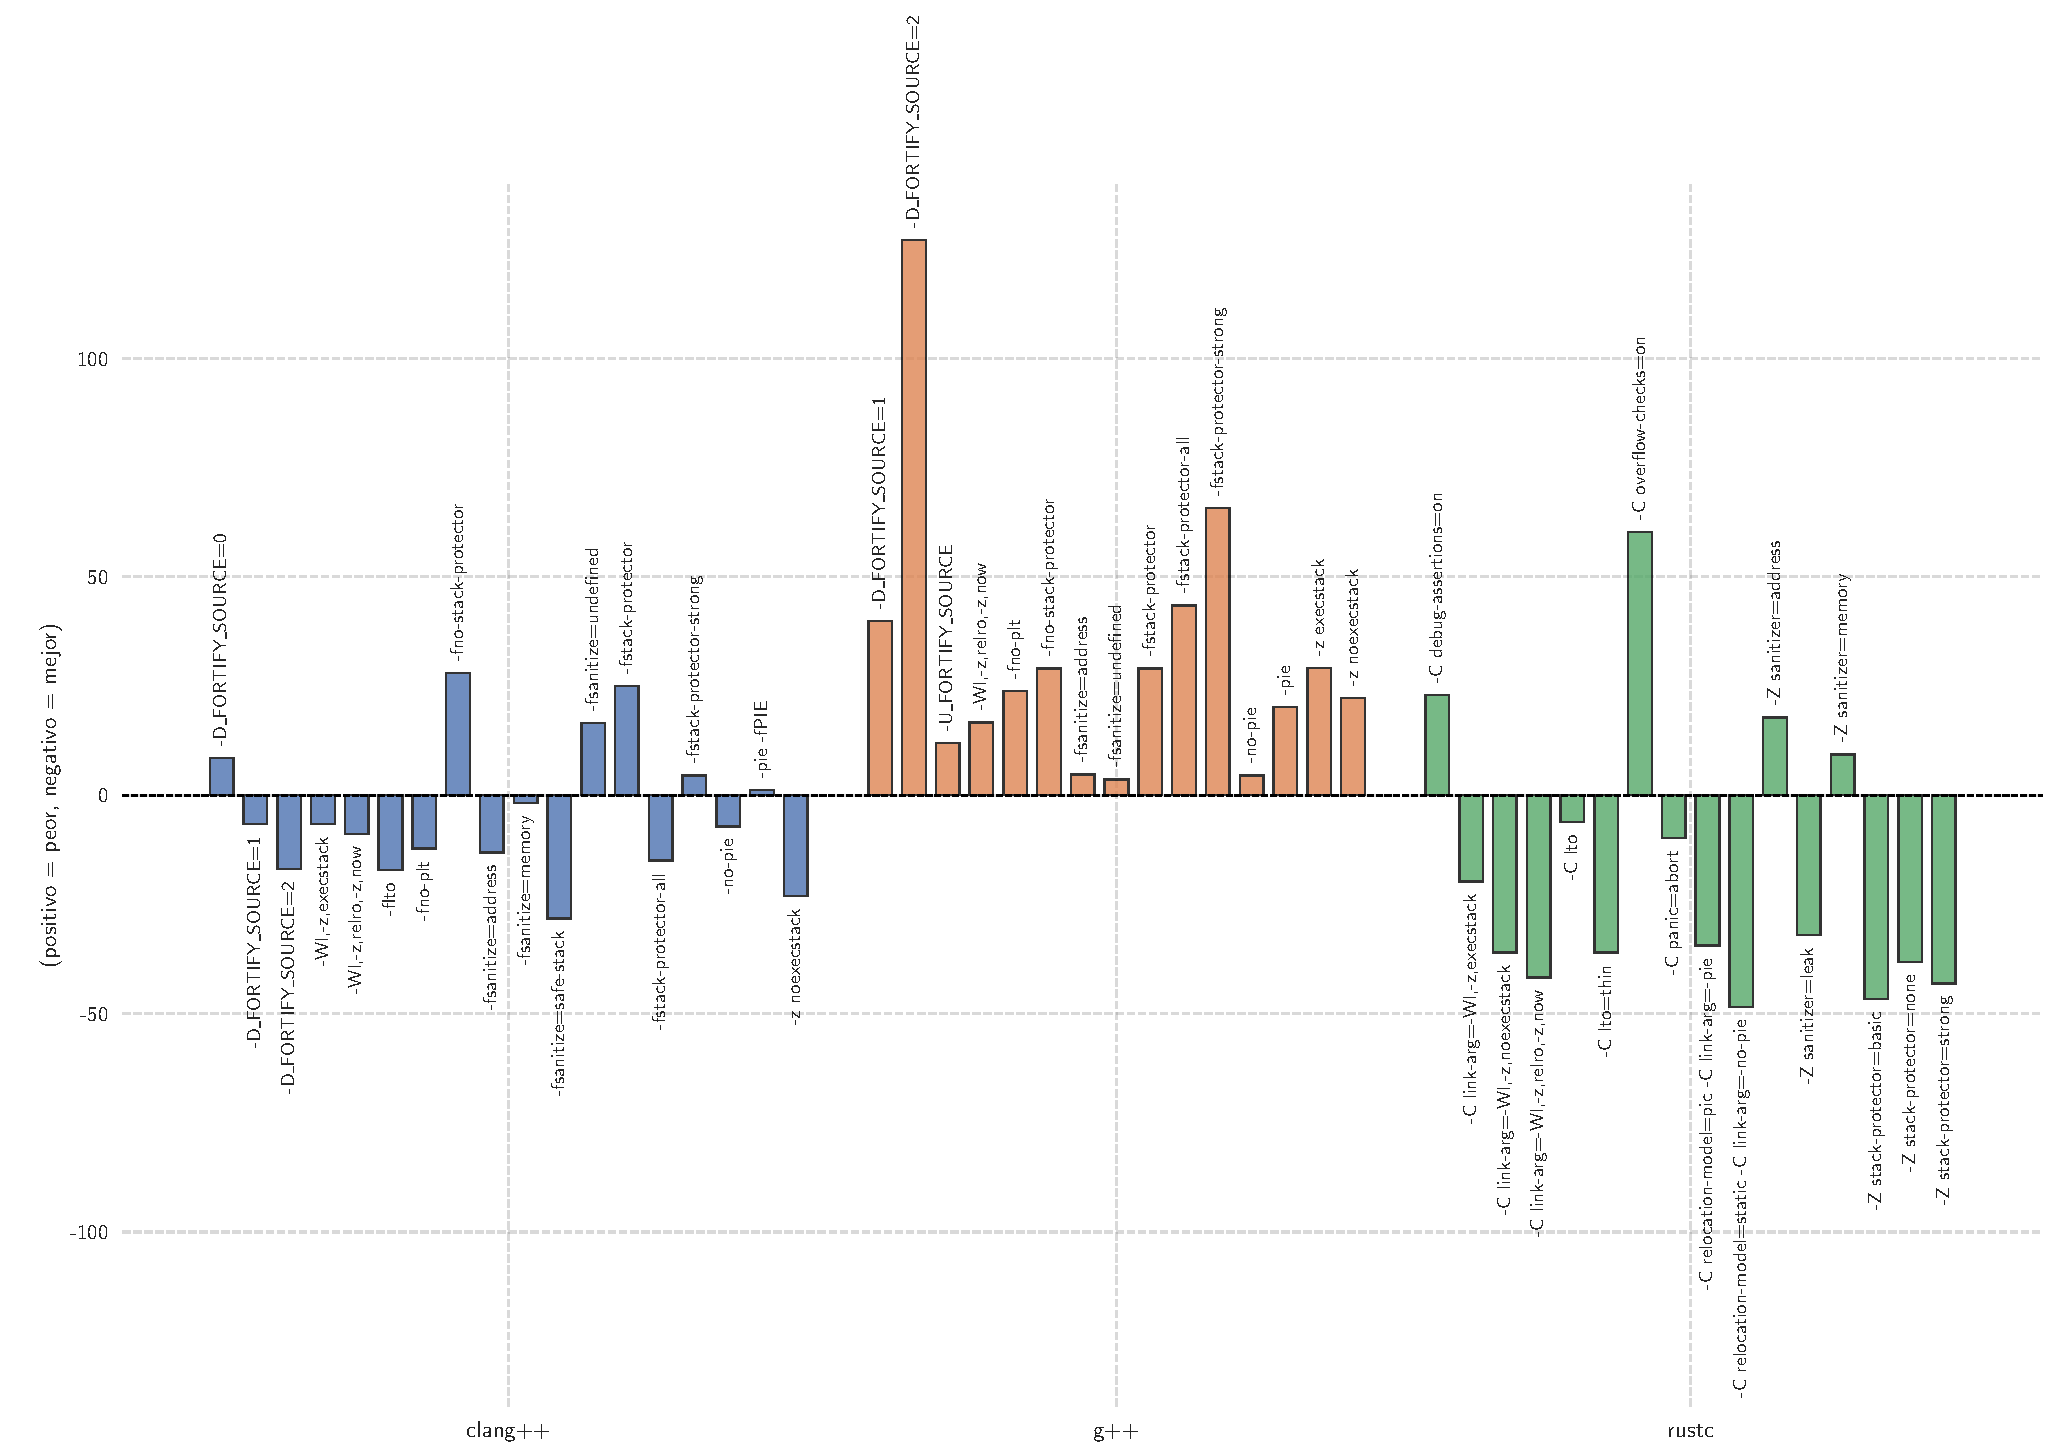
\includegraphics[width=\linewidth]{Gráficas/Gráficas_por_optimización_porcentual/-O2/Time_ms.pdf}
      \label{fig:Gráficas_gráficas_por_optimización_porcentual__o2_time_ms}
    }
  \end{minipage}

\end{figure}
\newpage

% === Gráficas_por_optimización_porcentual/-O3 ===
\subsection*{-O3}
\begin{figure}[htbp]
  \centering
  \caption{Resultados de compilación con optimización \texttt{-O3}}
  \vspace{0.5cm}

  \begin{minipage}{0.48\textwidth}
    \centering
    \subfloat[Tamaño del archivo (KB)]{
      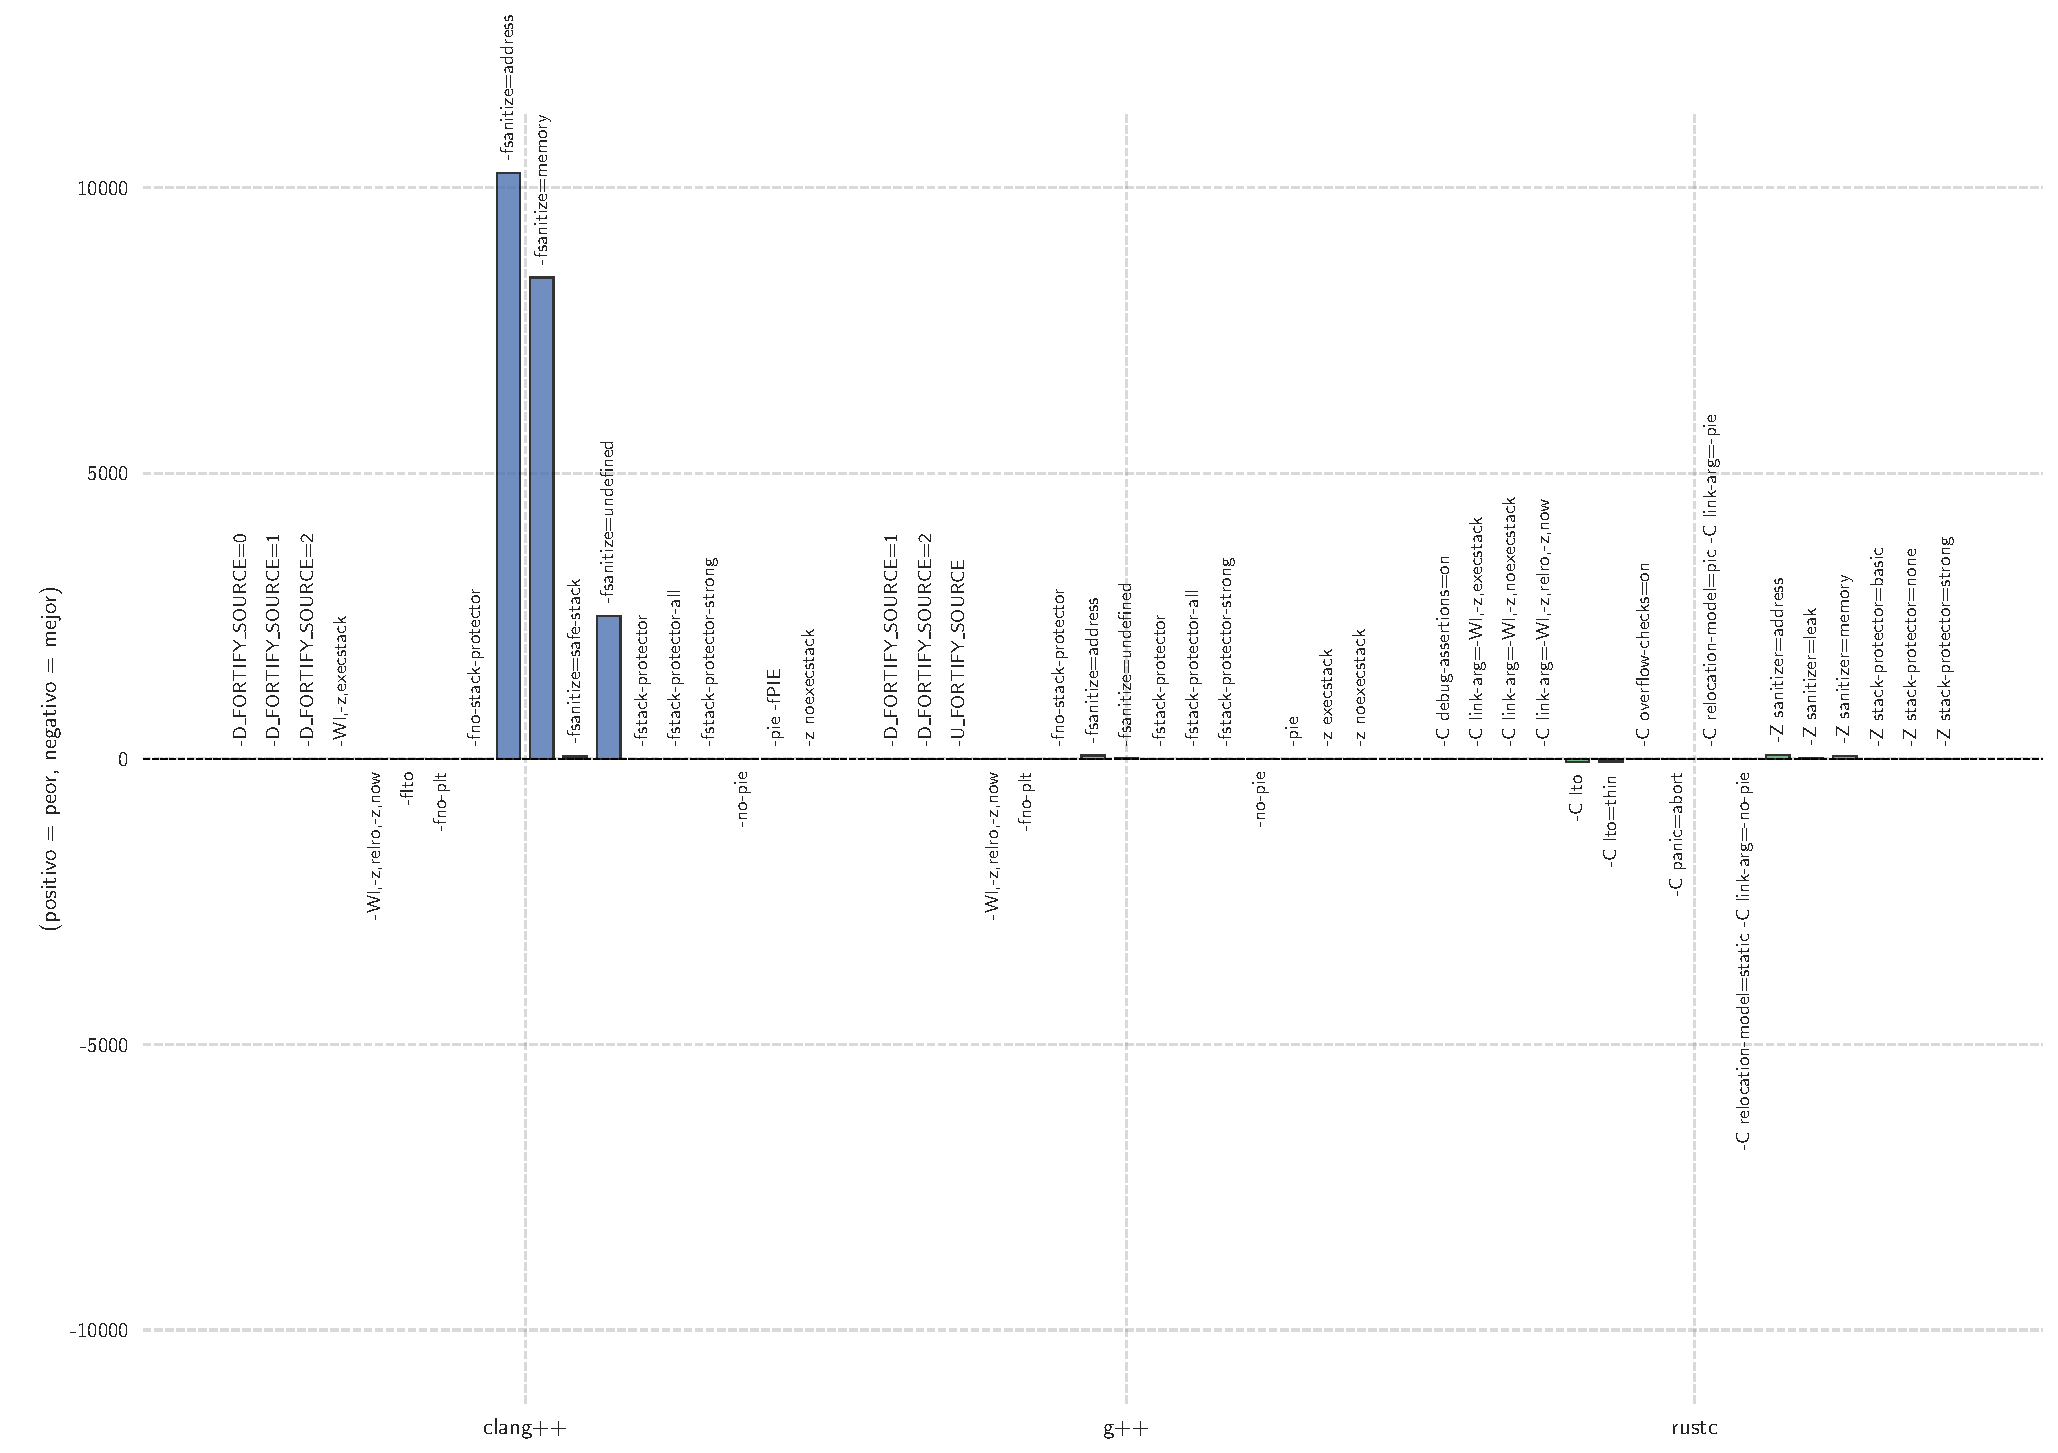
\includegraphics[width=\linewidth]{Gráficas/Gráficas_por_optimización_porcentual/-O3/File_size_KB.pdf}
      \label{fig:Gráficas_gráficas_por_optimización_porcentual__o3_file_size_kb}
    }
  \end{minipage}
  \hfill
  \begin{minipage}{0.48\textwidth}
    \centering
    \subfloat[Funciones fortificadas (\%)]{
      \includegraphics[width=\linewidth]{Gráficas/Gráficas_por_optimización_porcentual/-O3/Fortified_Functions.pdf}
      \label{fig:Gráficas_gráficas_por_optimización_porcentual__o3_fortified_functions}
    }
  \end{minipage}


  \vspace{1cm}

  \begin{minipage}{0.48\textwidth}
    \centering
    \subfloat[Uso de memoria (KB)]{
      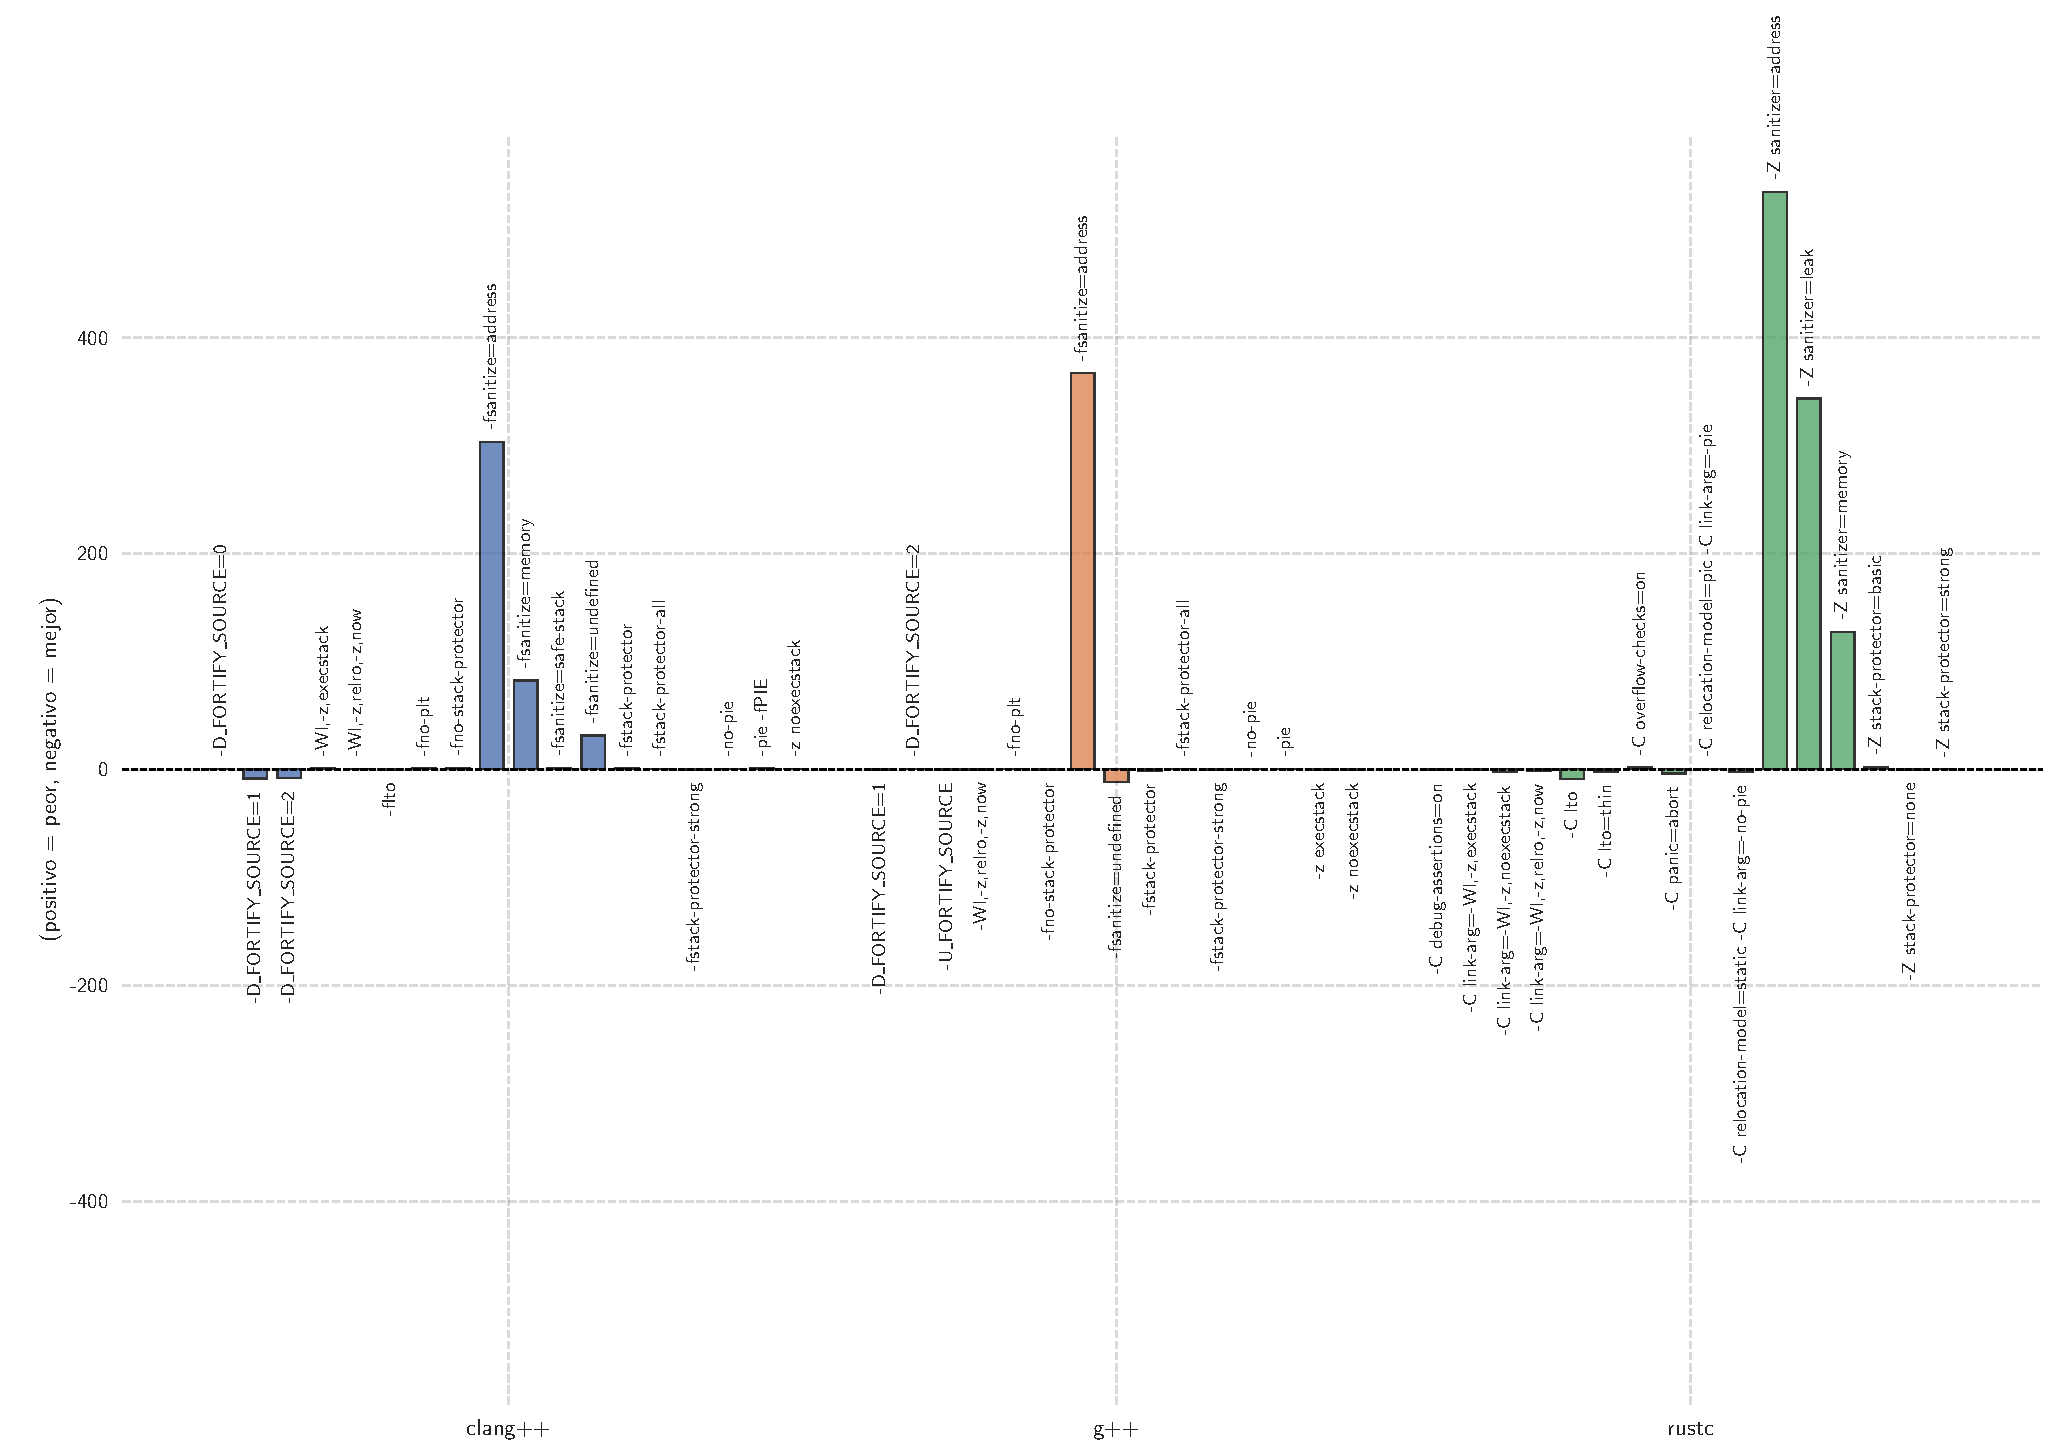
\includegraphics[width=\linewidth]{Gráficas/Gráficas_por_optimización_porcentual/-O3/Memory_usage_KB.pdf}
      \label{fig:Gráficas_gráficas_por_optimización_porcentual__o3_memory_usage_kb}
    }
  \end{minipage}
  \hfill
  \begin{minipage}{0.48\textwidth}
    \centering
    \subfloat[Tiempo (ms)]{
      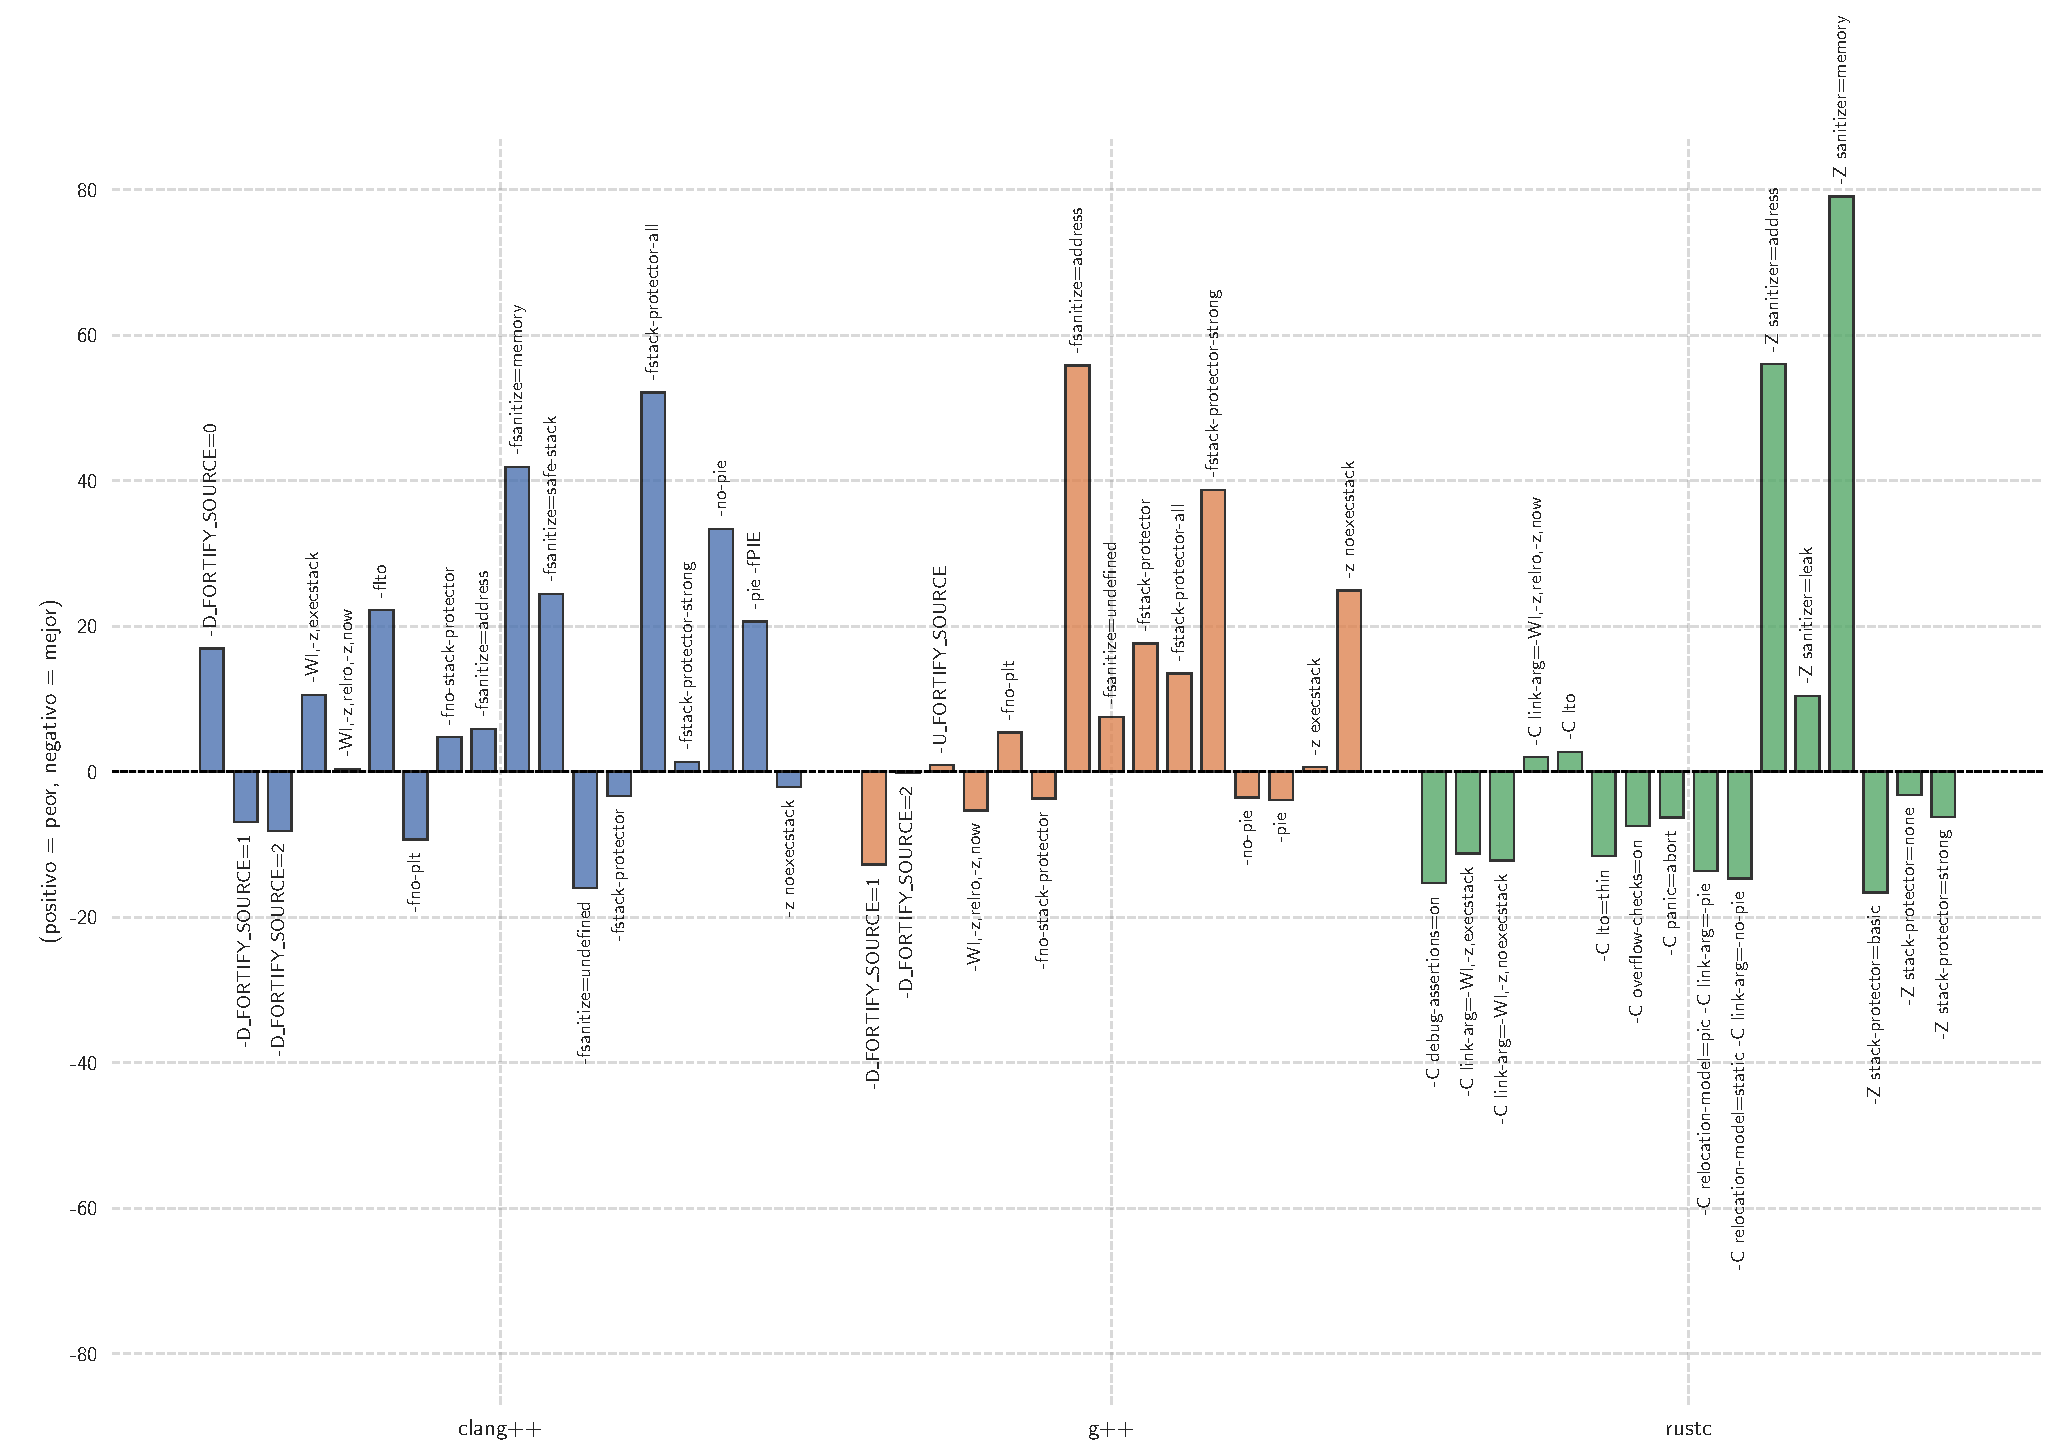
\includegraphics[width=\linewidth]{Gráficas/Gráficas_por_optimización_porcentual/-O3/Time_ms.pdf}
      \label{fig:Gráficas_gráficas_por_optimización_porcentual__o3_time_ms}
    }
  \end{minipage}

\end{figure}
\newpage

% === Gráficas_por_optimización_porcentual/-Ofast ===
\subsection*{-OFAST}
\begin{figure}[htbp]
  \centering
  \caption{Resultados de compilación con optimización \texttt{-Ofast}}
  \vspace{0.5cm}

  \begin{minipage}{0.48\textwidth}
    \centering
    \subfloat[Tamaño del archivo (KB)]{
      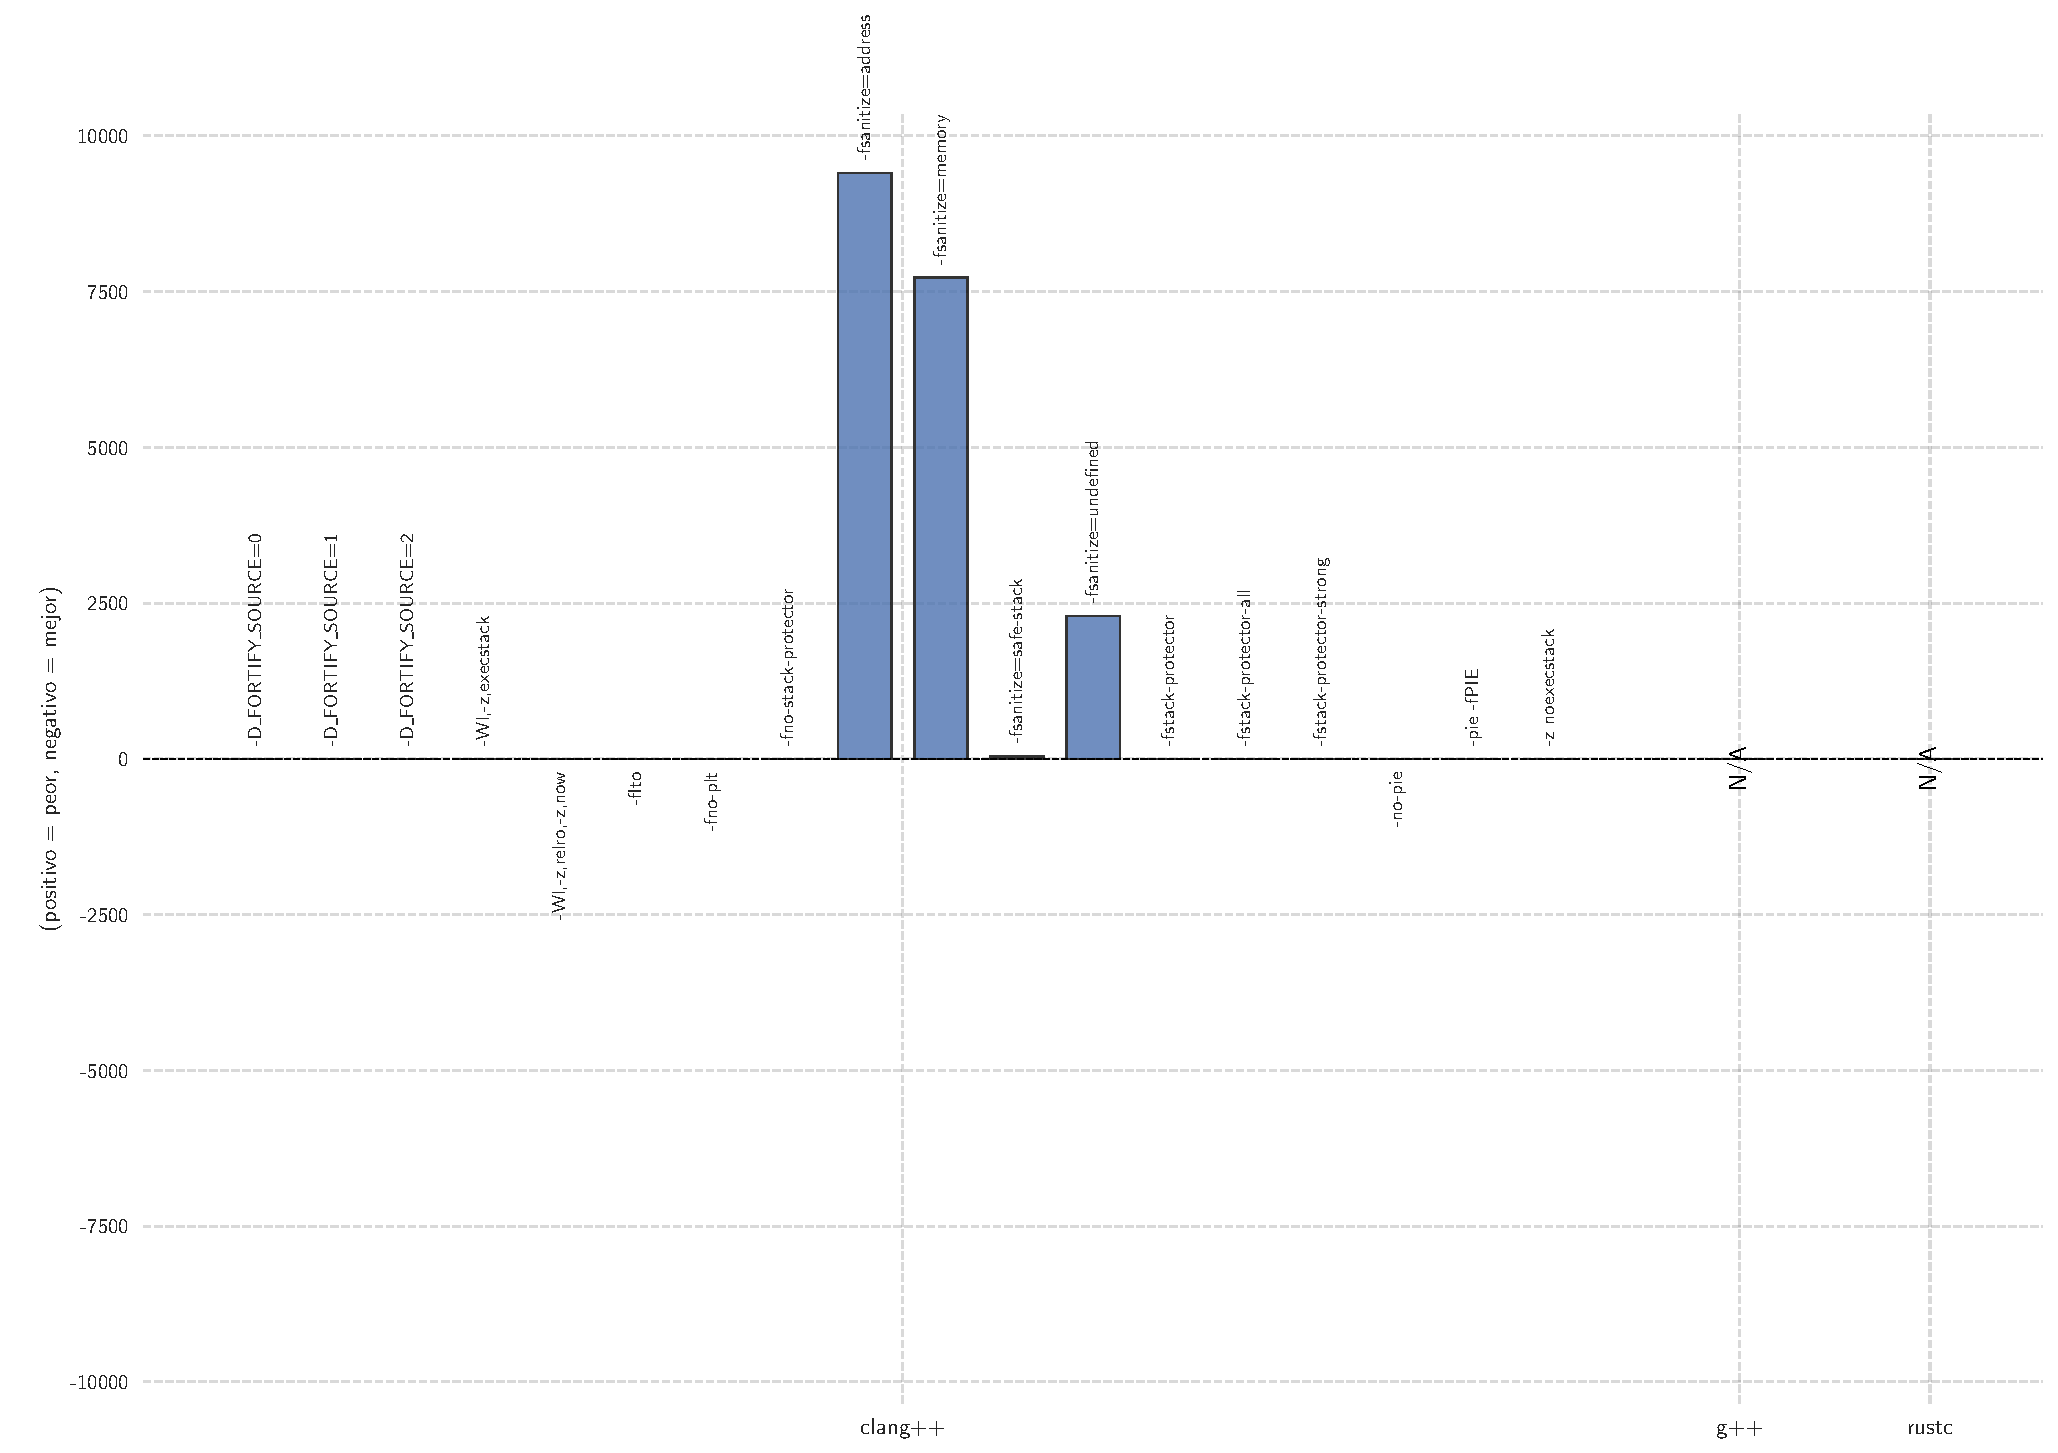
\includegraphics[width=\linewidth]{Gráficas/Gráficas_por_optimización_porcentual/-Ofast/File_size_KB.pdf}
      \label{fig:Gráficas_gráficas_por_optimización_porcentual__ofast_file_size_kb}
    }
  \end{minipage}
  \hfill
  \begin{minipage}{0.48\textwidth}
    \centering
    \subfloat[Funciones fortificadas (\%)]{
      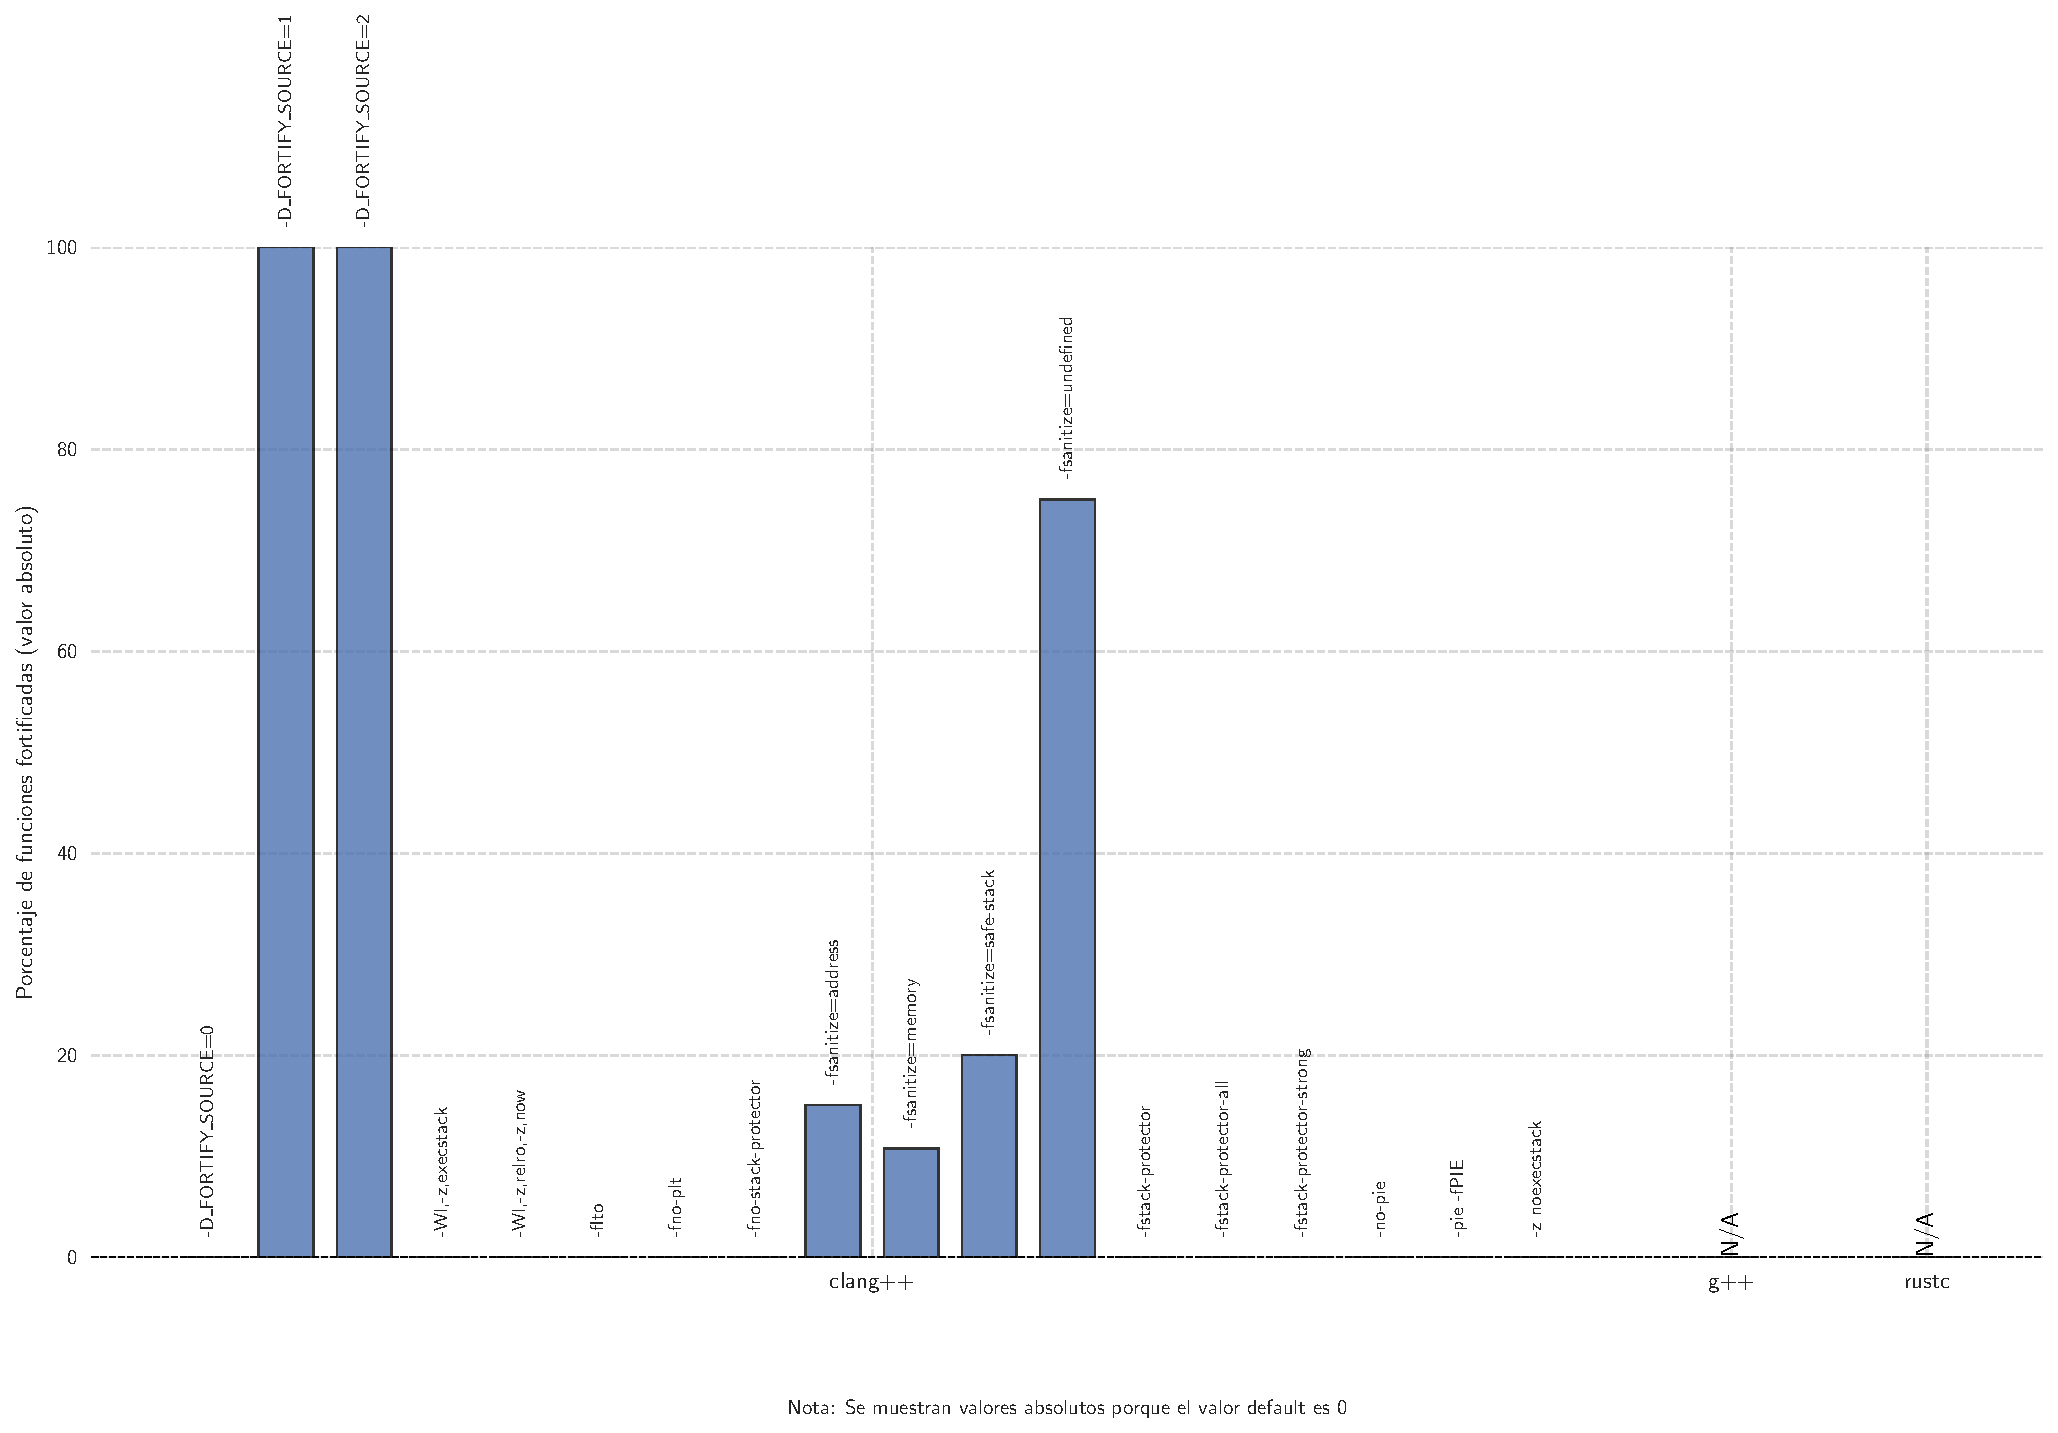
\includegraphics[width=\linewidth]{Gráficas/Gráficas_por_optimización_porcentual/-Ofast/Fortified_Functions.pdf}
      \label{fig:Gráficas_gráficas_por_optimización_porcentual__ofast_fortified_functions}
    }
  \end{minipage}


  \vspace{1cm}

  \begin{minipage}{0.48\textwidth}
    \centering
    \subfloat[Uso de memoria (KB)]{
      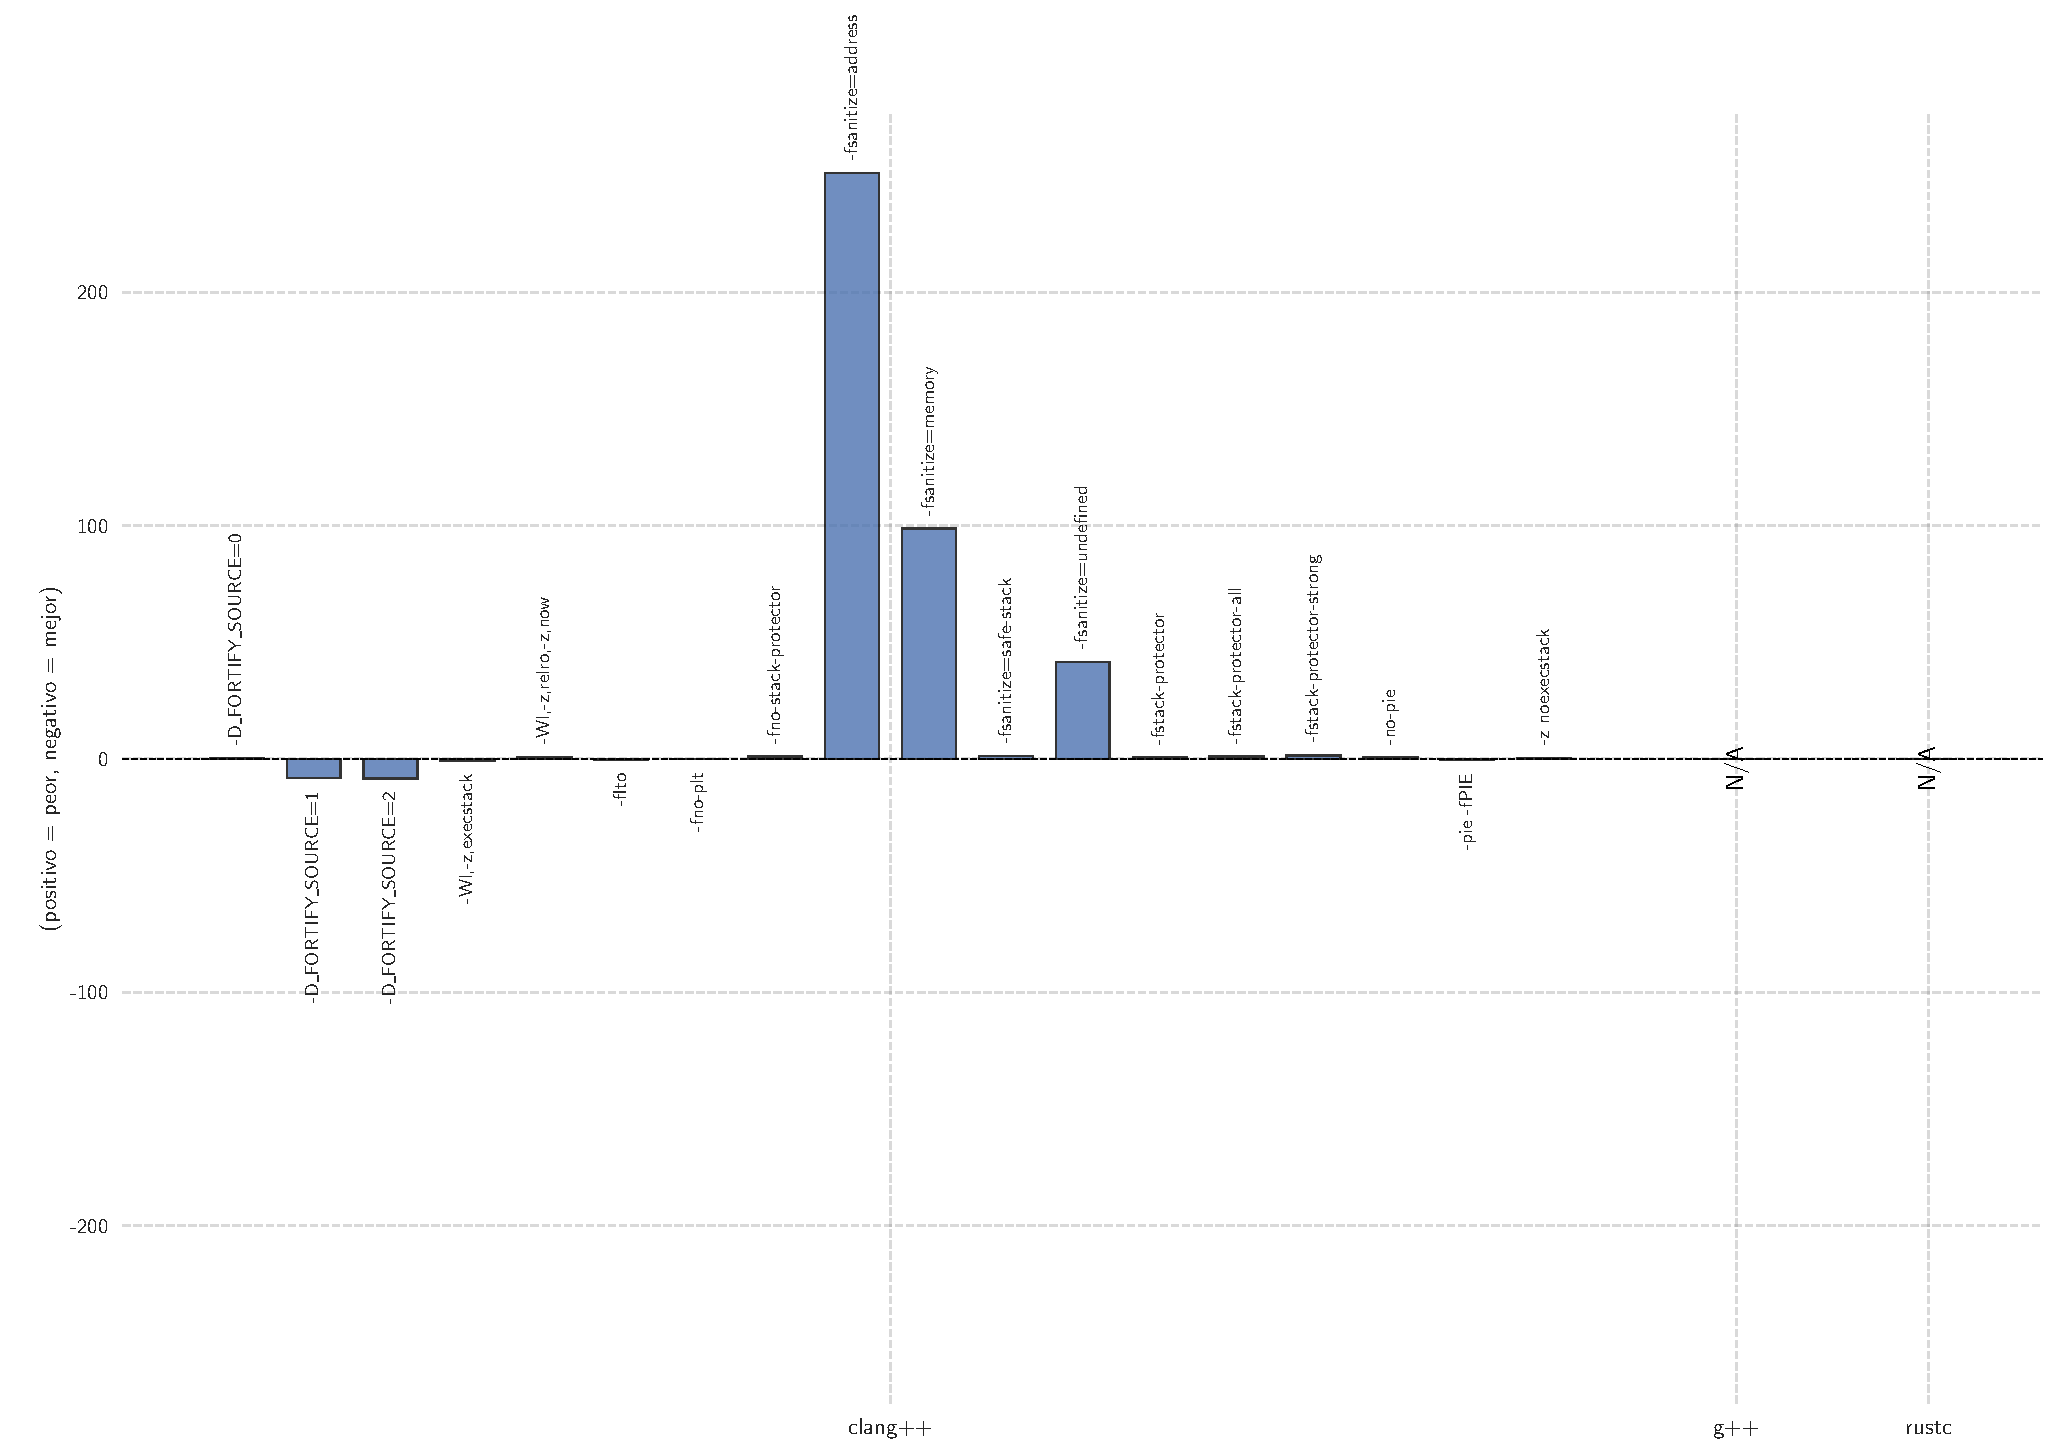
\includegraphics[width=\linewidth]{Gráficas/Gráficas_por_optimización_porcentual/-Ofast/Memory_usage_KB.pdf}
      \label{fig:Gráficas_gráficas_por_optimización_porcentual__ofast_memory_usage_kb}
    }
  \end{minipage}
  \hfill
  \begin{minipage}{0.48\textwidth}
    \centering
    \subfloat[Tiempo (ms)]{
      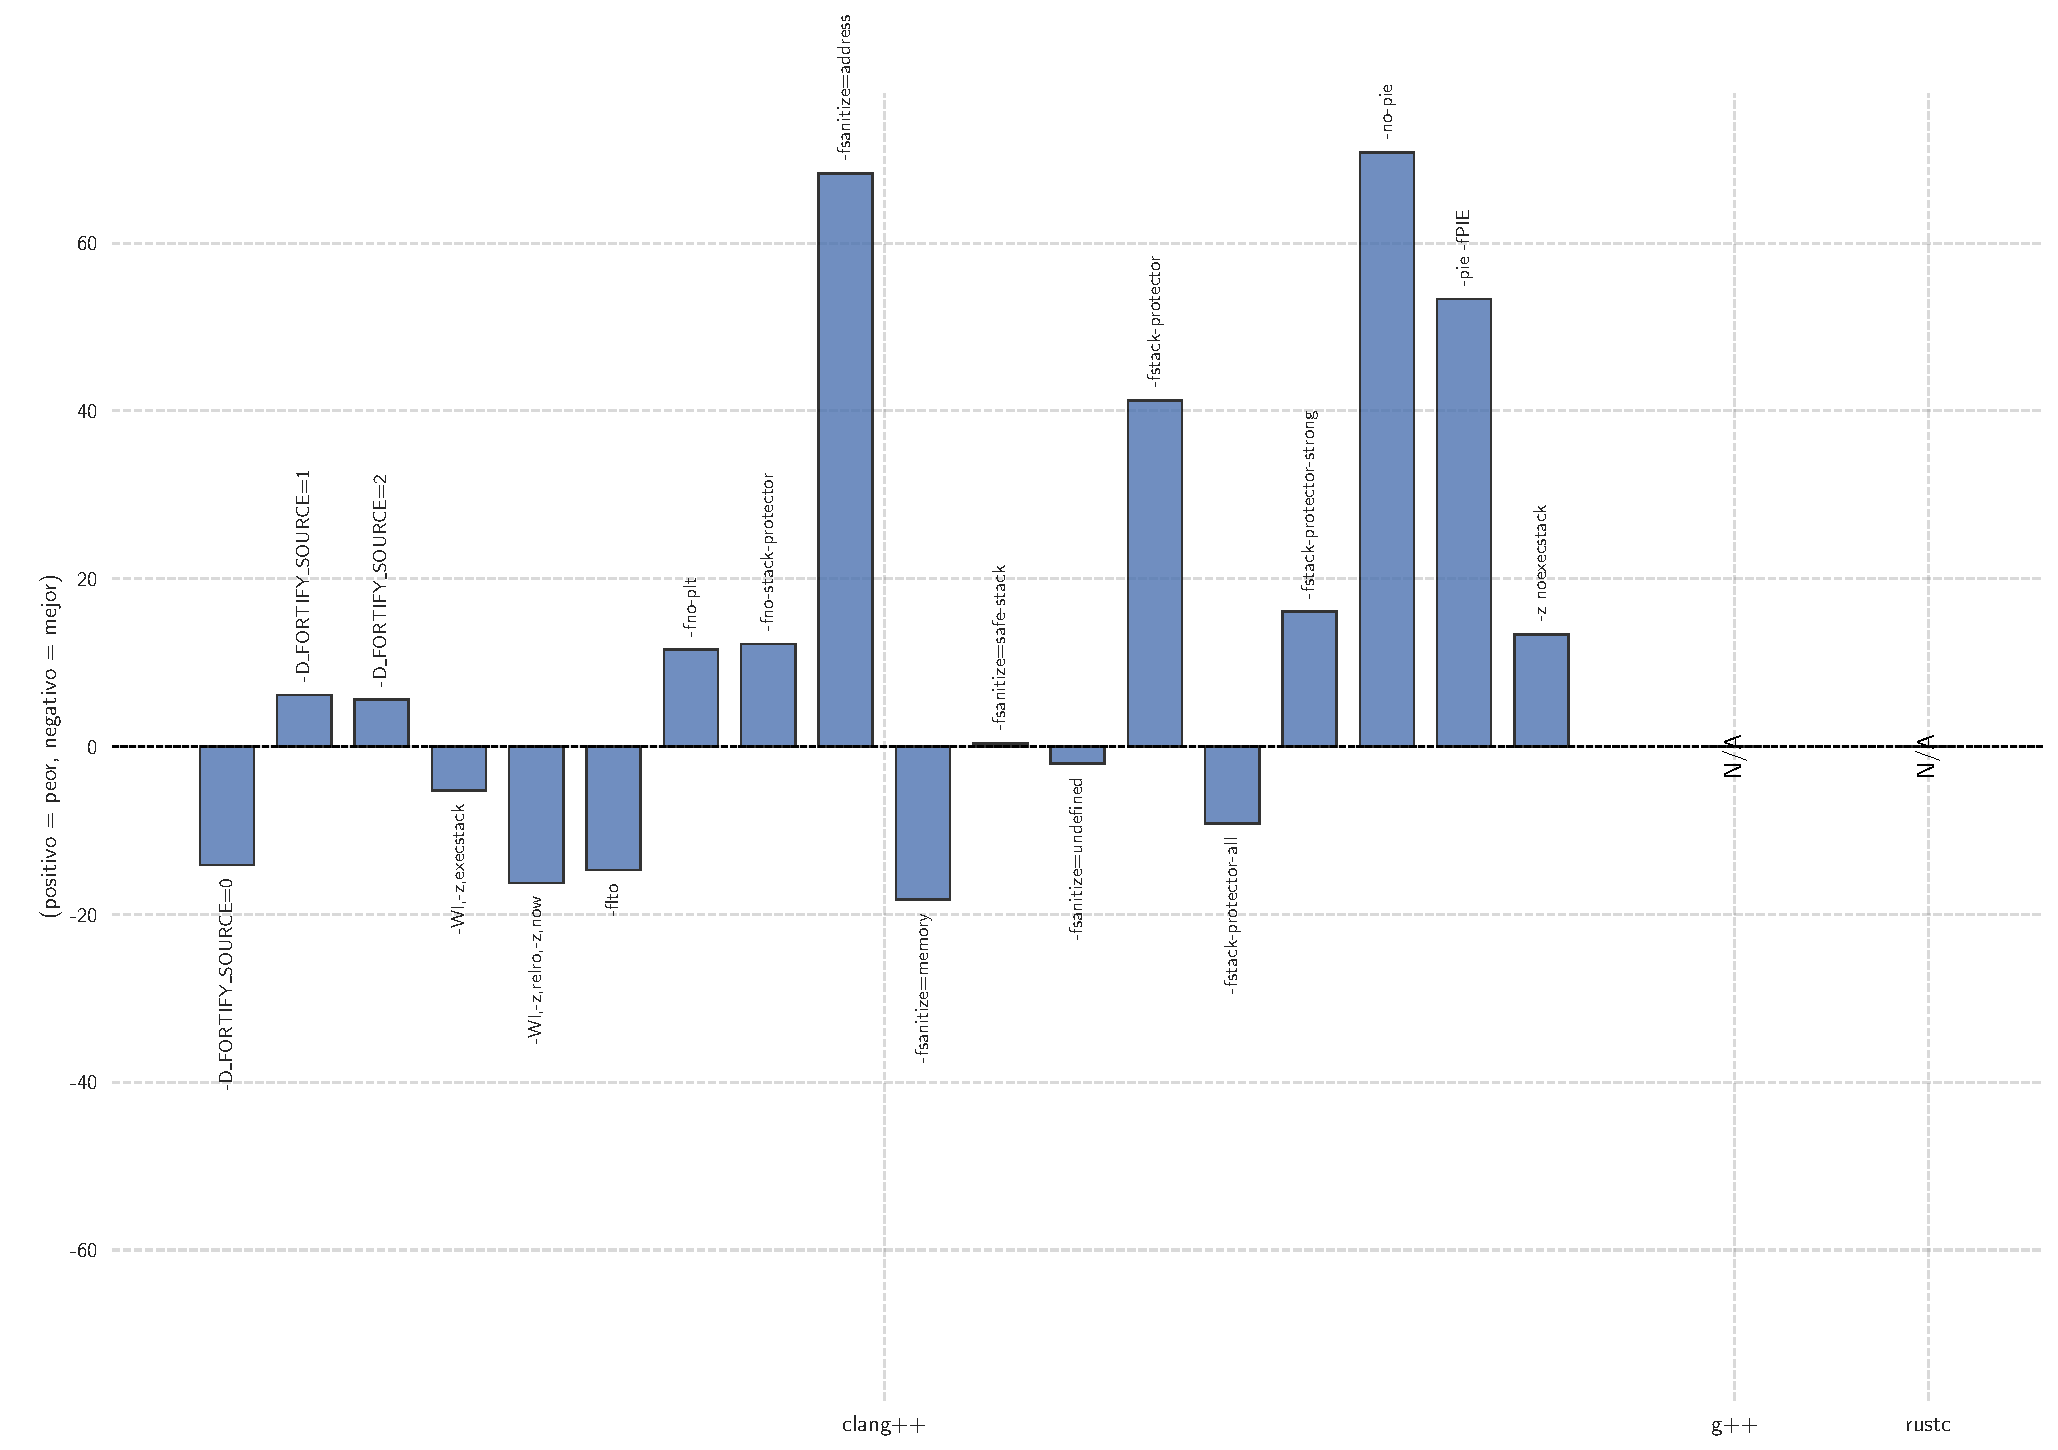
\includegraphics[width=\linewidth]{Gráficas/Gráficas_por_optimización_porcentual/-Ofast/Time_ms.pdf}
      \label{fig:Gráficas_gráficas_por_optimización_porcentual__ofast_time_ms}
    }
  \end{minipage}

\end{figure}
\newpage

% === Gráficas_por_optimización_porcentual/-Os ===
\subsection*{-OS}
\begin{figure}[htbp]
  \centering
  \caption{Resultados de compilación con optimización \texttt{-Os}}
  \vspace{0.5cm}

  \begin{minipage}{0.48\textwidth}
    \centering
    \subfloat[Tamaño del archivo (KB)]{
      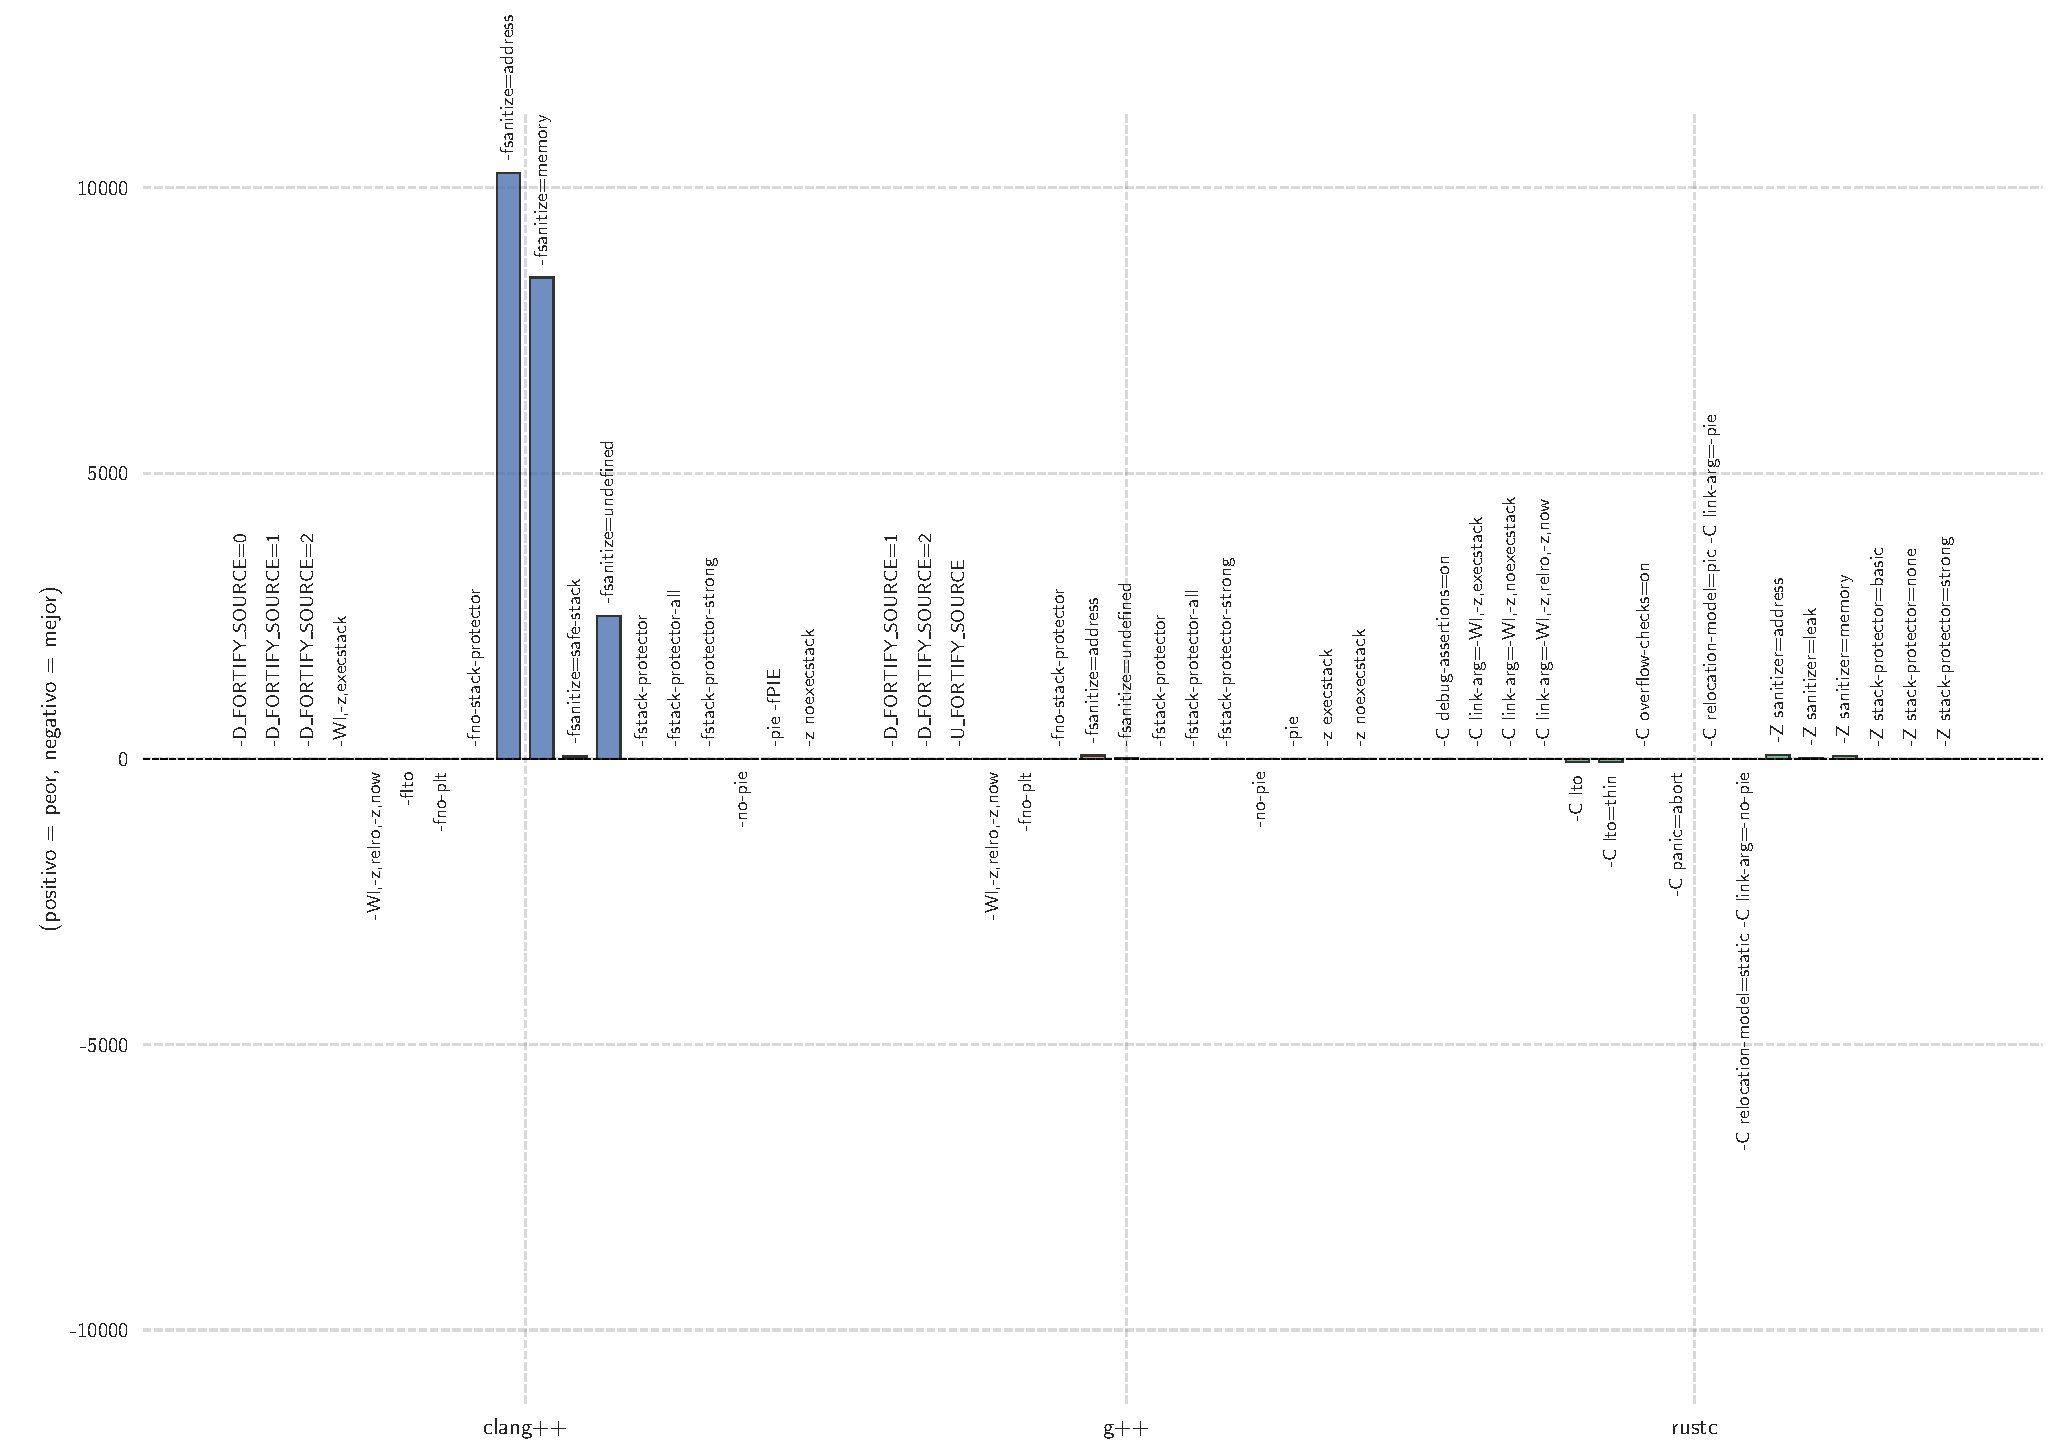
\includegraphics[width=\linewidth]{Gráficas/Gráficas_por_optimización_porcentual/-Os/File_size_KB.pdf}
      \label{fig:Gráficas_gráficas_por_optimización_porcentual__os_file_size_kb}
    }
  \end{minipage}
  \hfill
  \begin{minipage}{0.48\textwidth}
    \centering
    \subfloat[Funciones fortificadas (\%)]{
      \includegraphics[width=\linewidth]{Gráficas/Gráficas_por_optimización_porcentual/-Os/Fortified_Functions.pdf}
      \label{fig:Gráficas_gráficas_por_optimización_porcentual__os_fortified_functions}
    }
  \end{minipage}


  \vspace{1cm}

  \begin{minipage}{0.48\textwidth}
    \centering
    \subfloat[Uso de memoria (KB)]{
      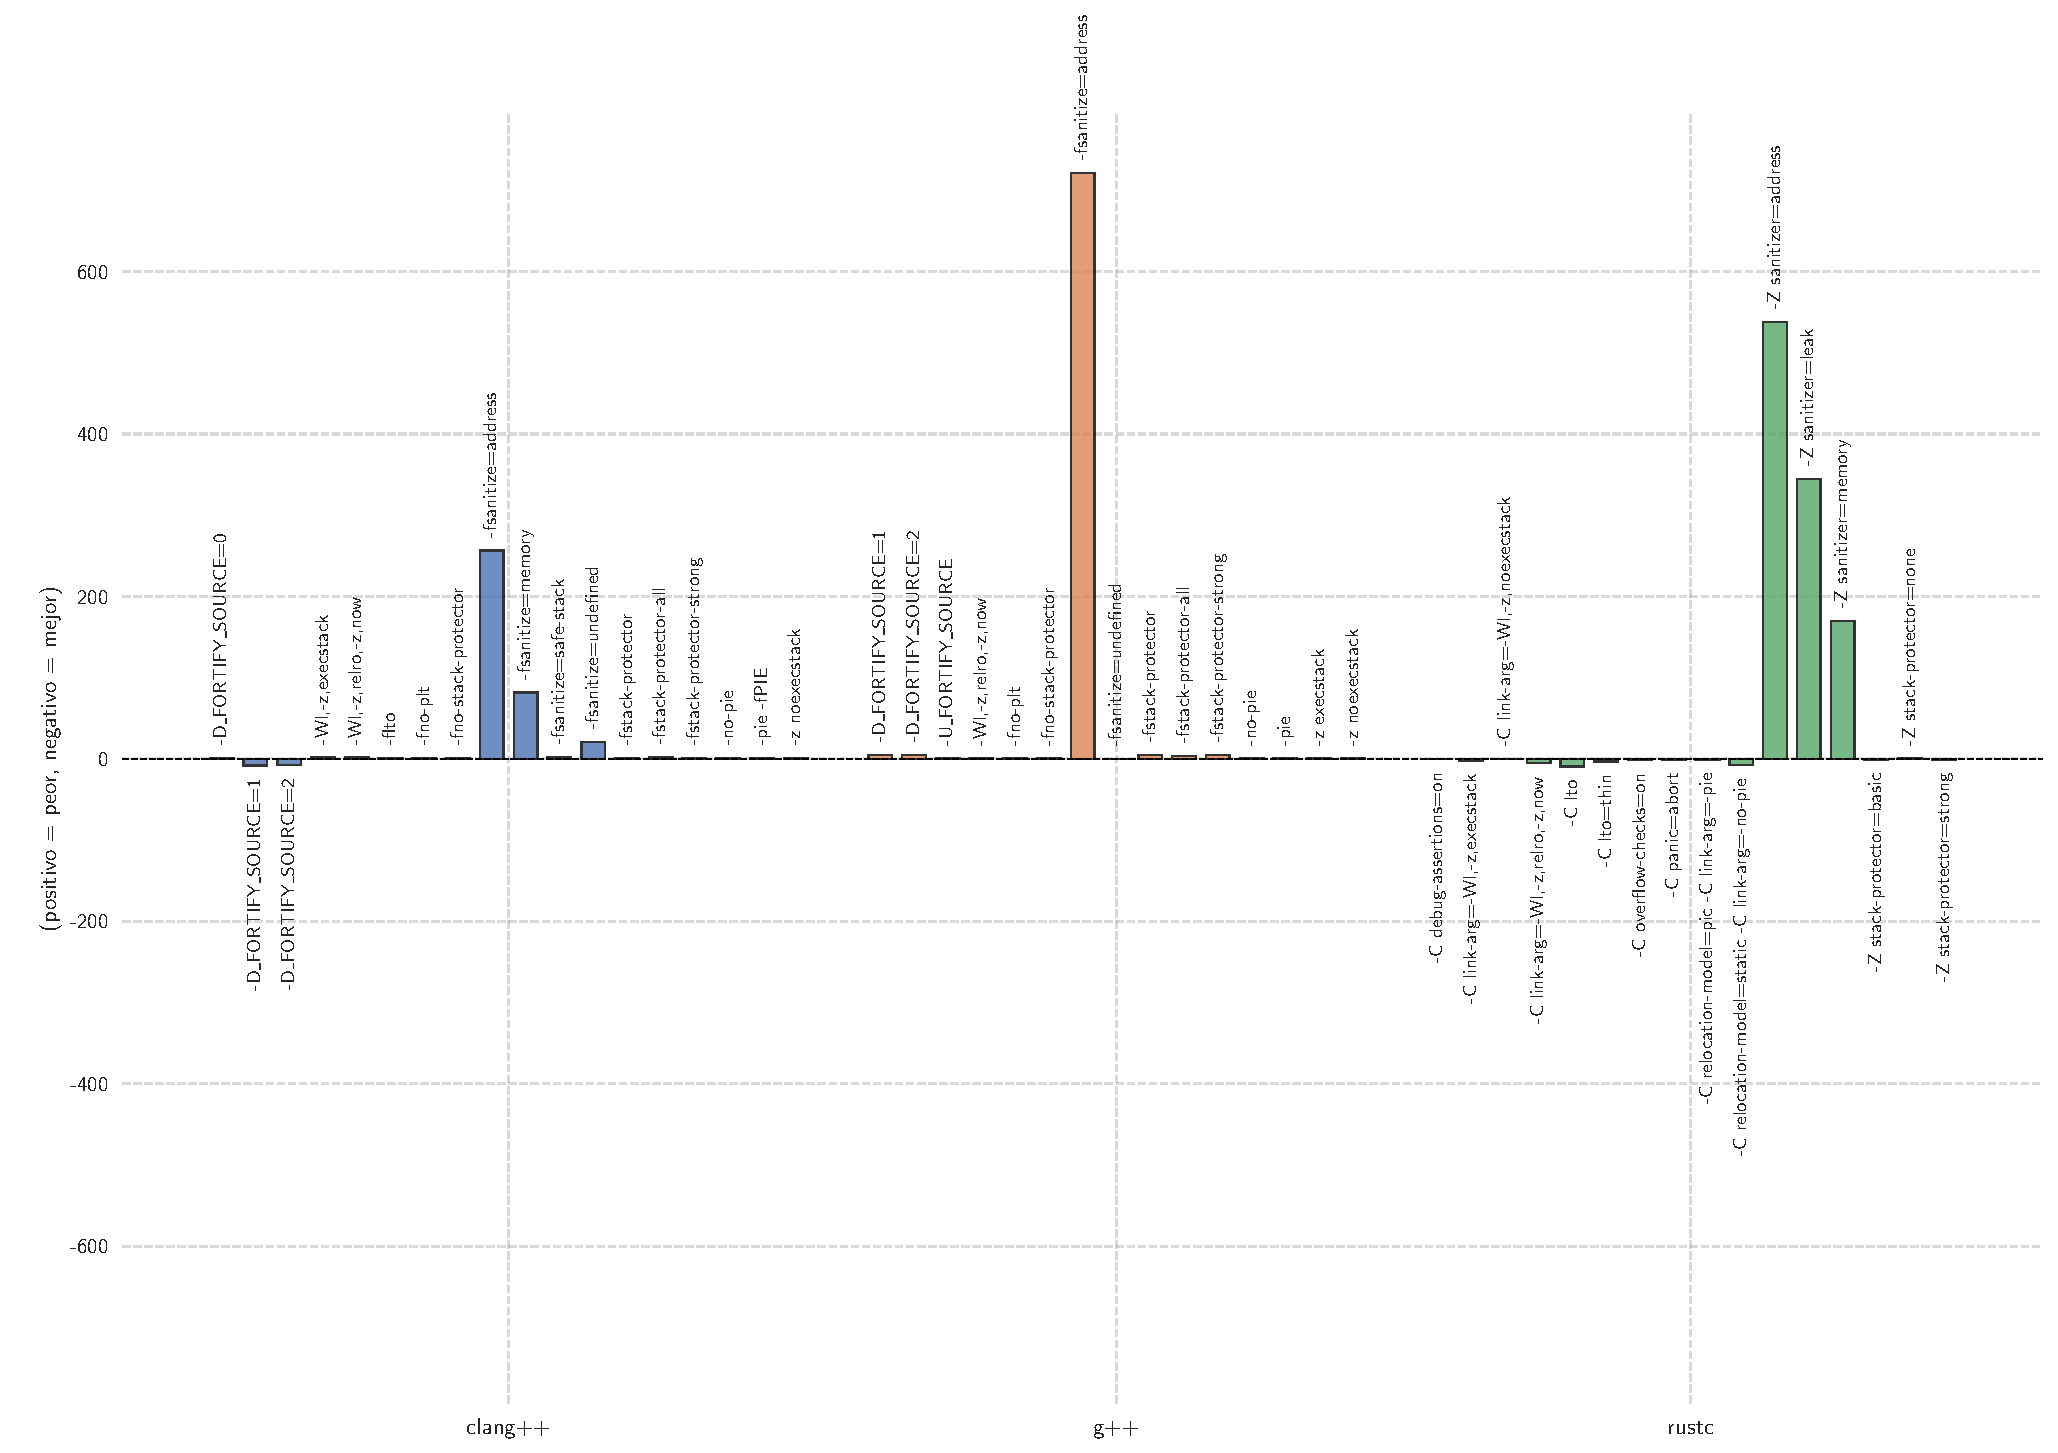
\includegraphics[width=\linewidth]{Gráficas/Gráficas_por_optimización_porcentual/-Os/Memory_usage_KB.pdf}
      \label{fig:Gráficas_gráficas_por_optimización_porcentual__os_memory_usage_kb}
    }
  \end{minipage}
  \hfill
  \begin{minipage}{0.48\textwidth}
    \centering
    \subfloat[Tiempo (ms)]{
      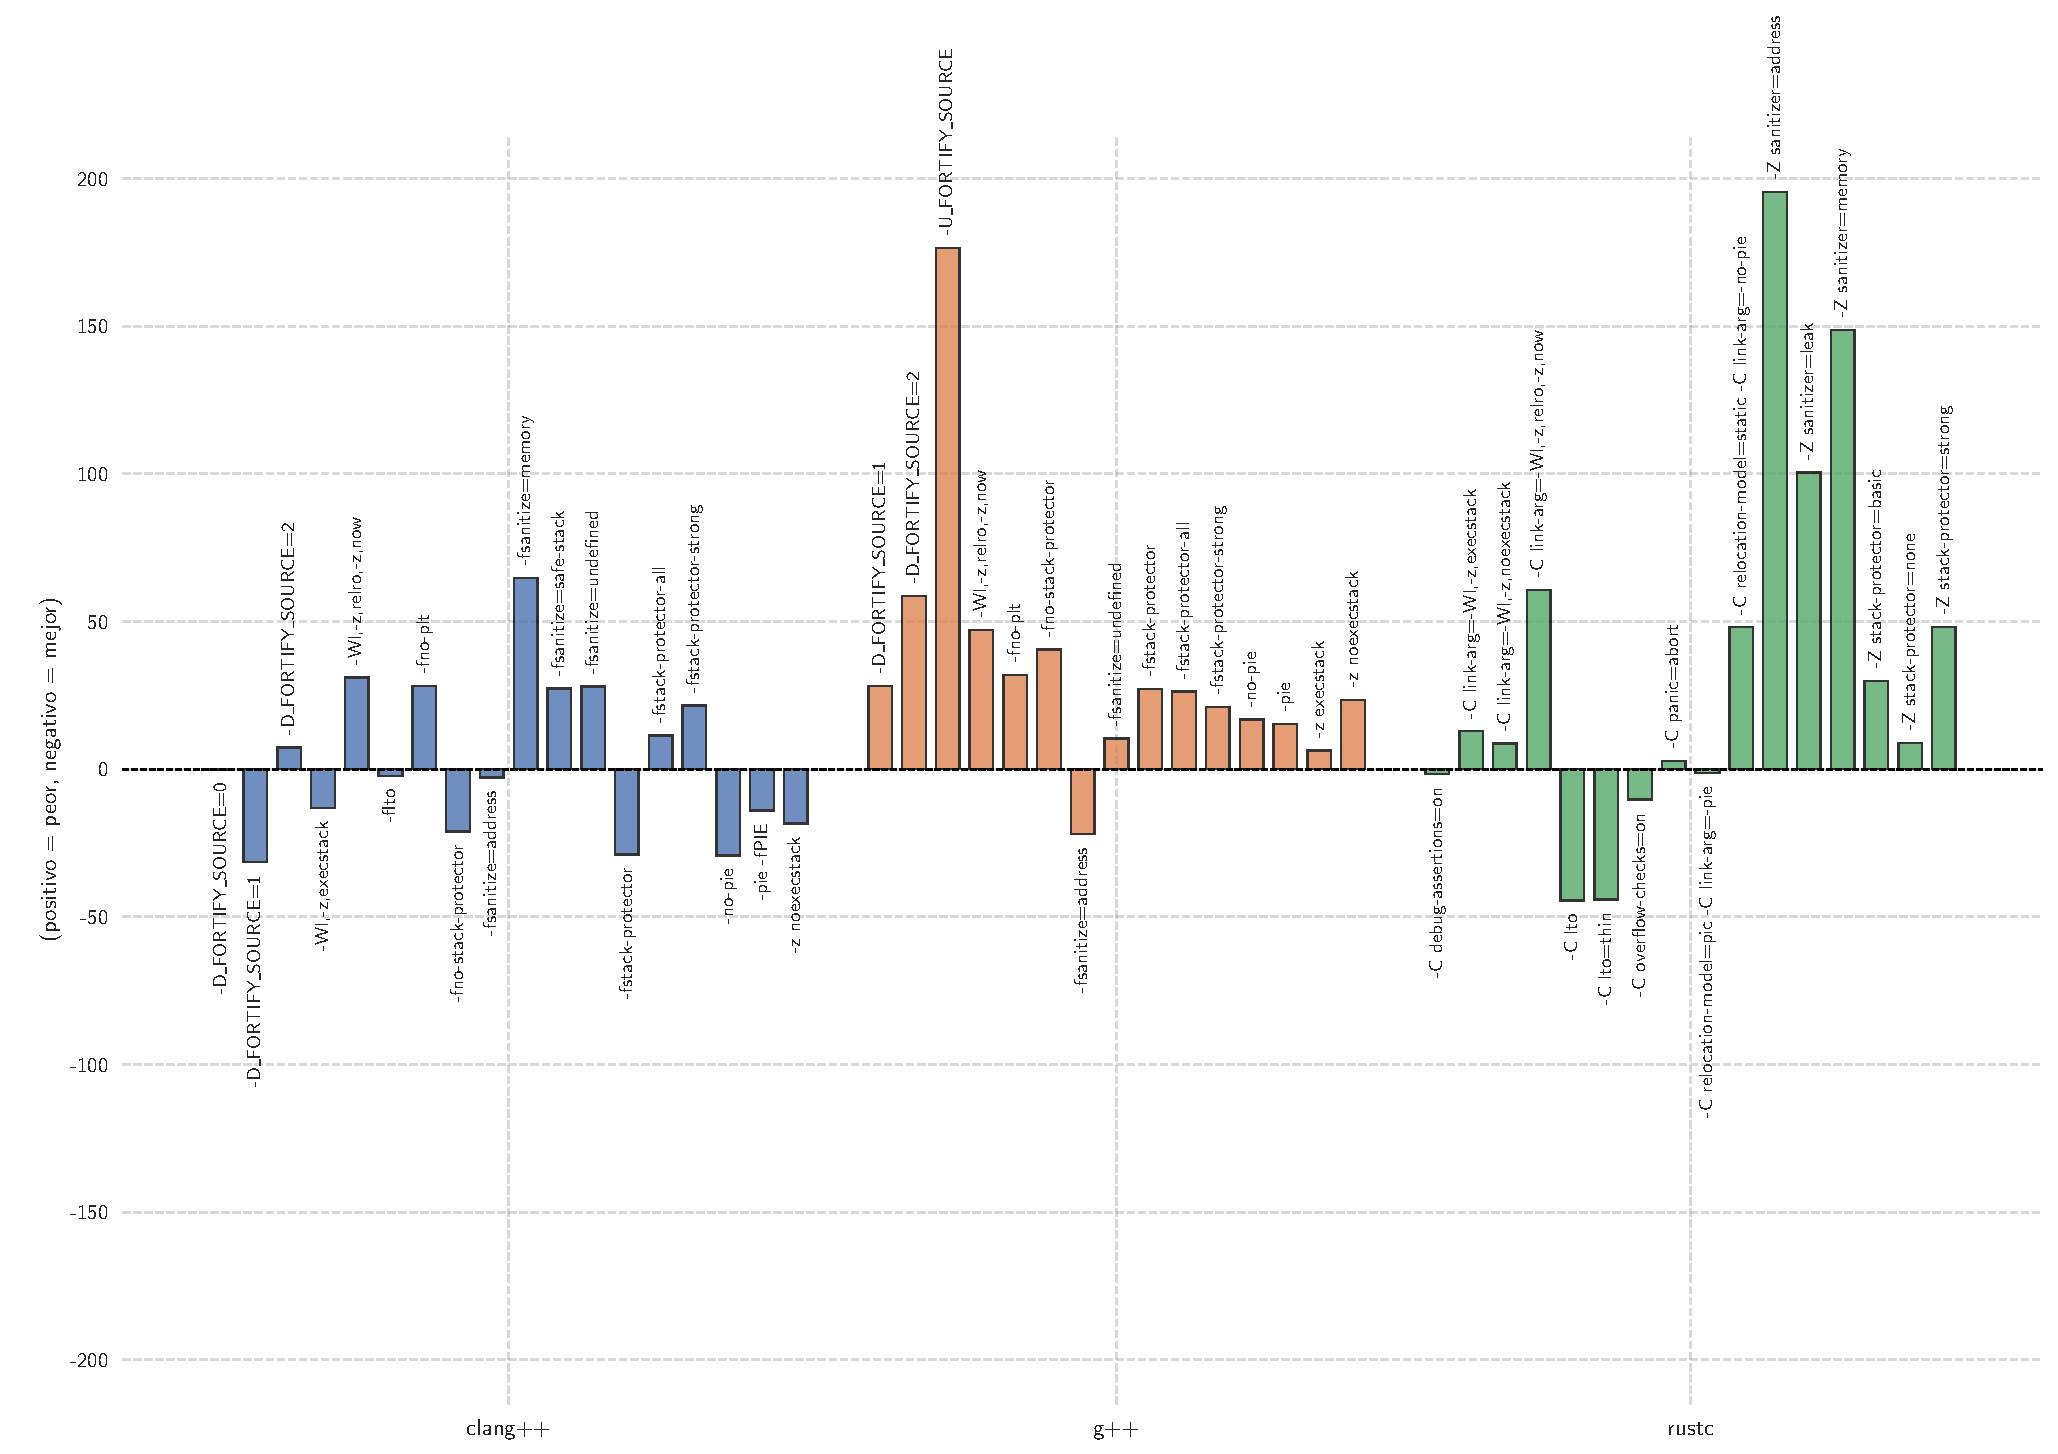
\includegraphics[width=\linewidth]{Gráficas/Gráficas_por_optimización_porcentual/-Os/Time_ms.pdf}
      \label{fig:Gráficas_gráficas_por_optimización_porcentual__os_time_ms}
    }
  \end{minipage}

\end{figure}
\newpage

% === Gráficas_por_optimización_porcentual/-Oz ===
\subsection*{-OZ}
\begin{figure}[htbp]
  \centering
  \caption{Resultados de compilación con optimización \texttt{-Oz}}
  \vspace{0.5cm}

  \begin{minipage}{0.48\textwidth}
    \centering
    \subfloat[Tamaño del archivo (KB)]{
      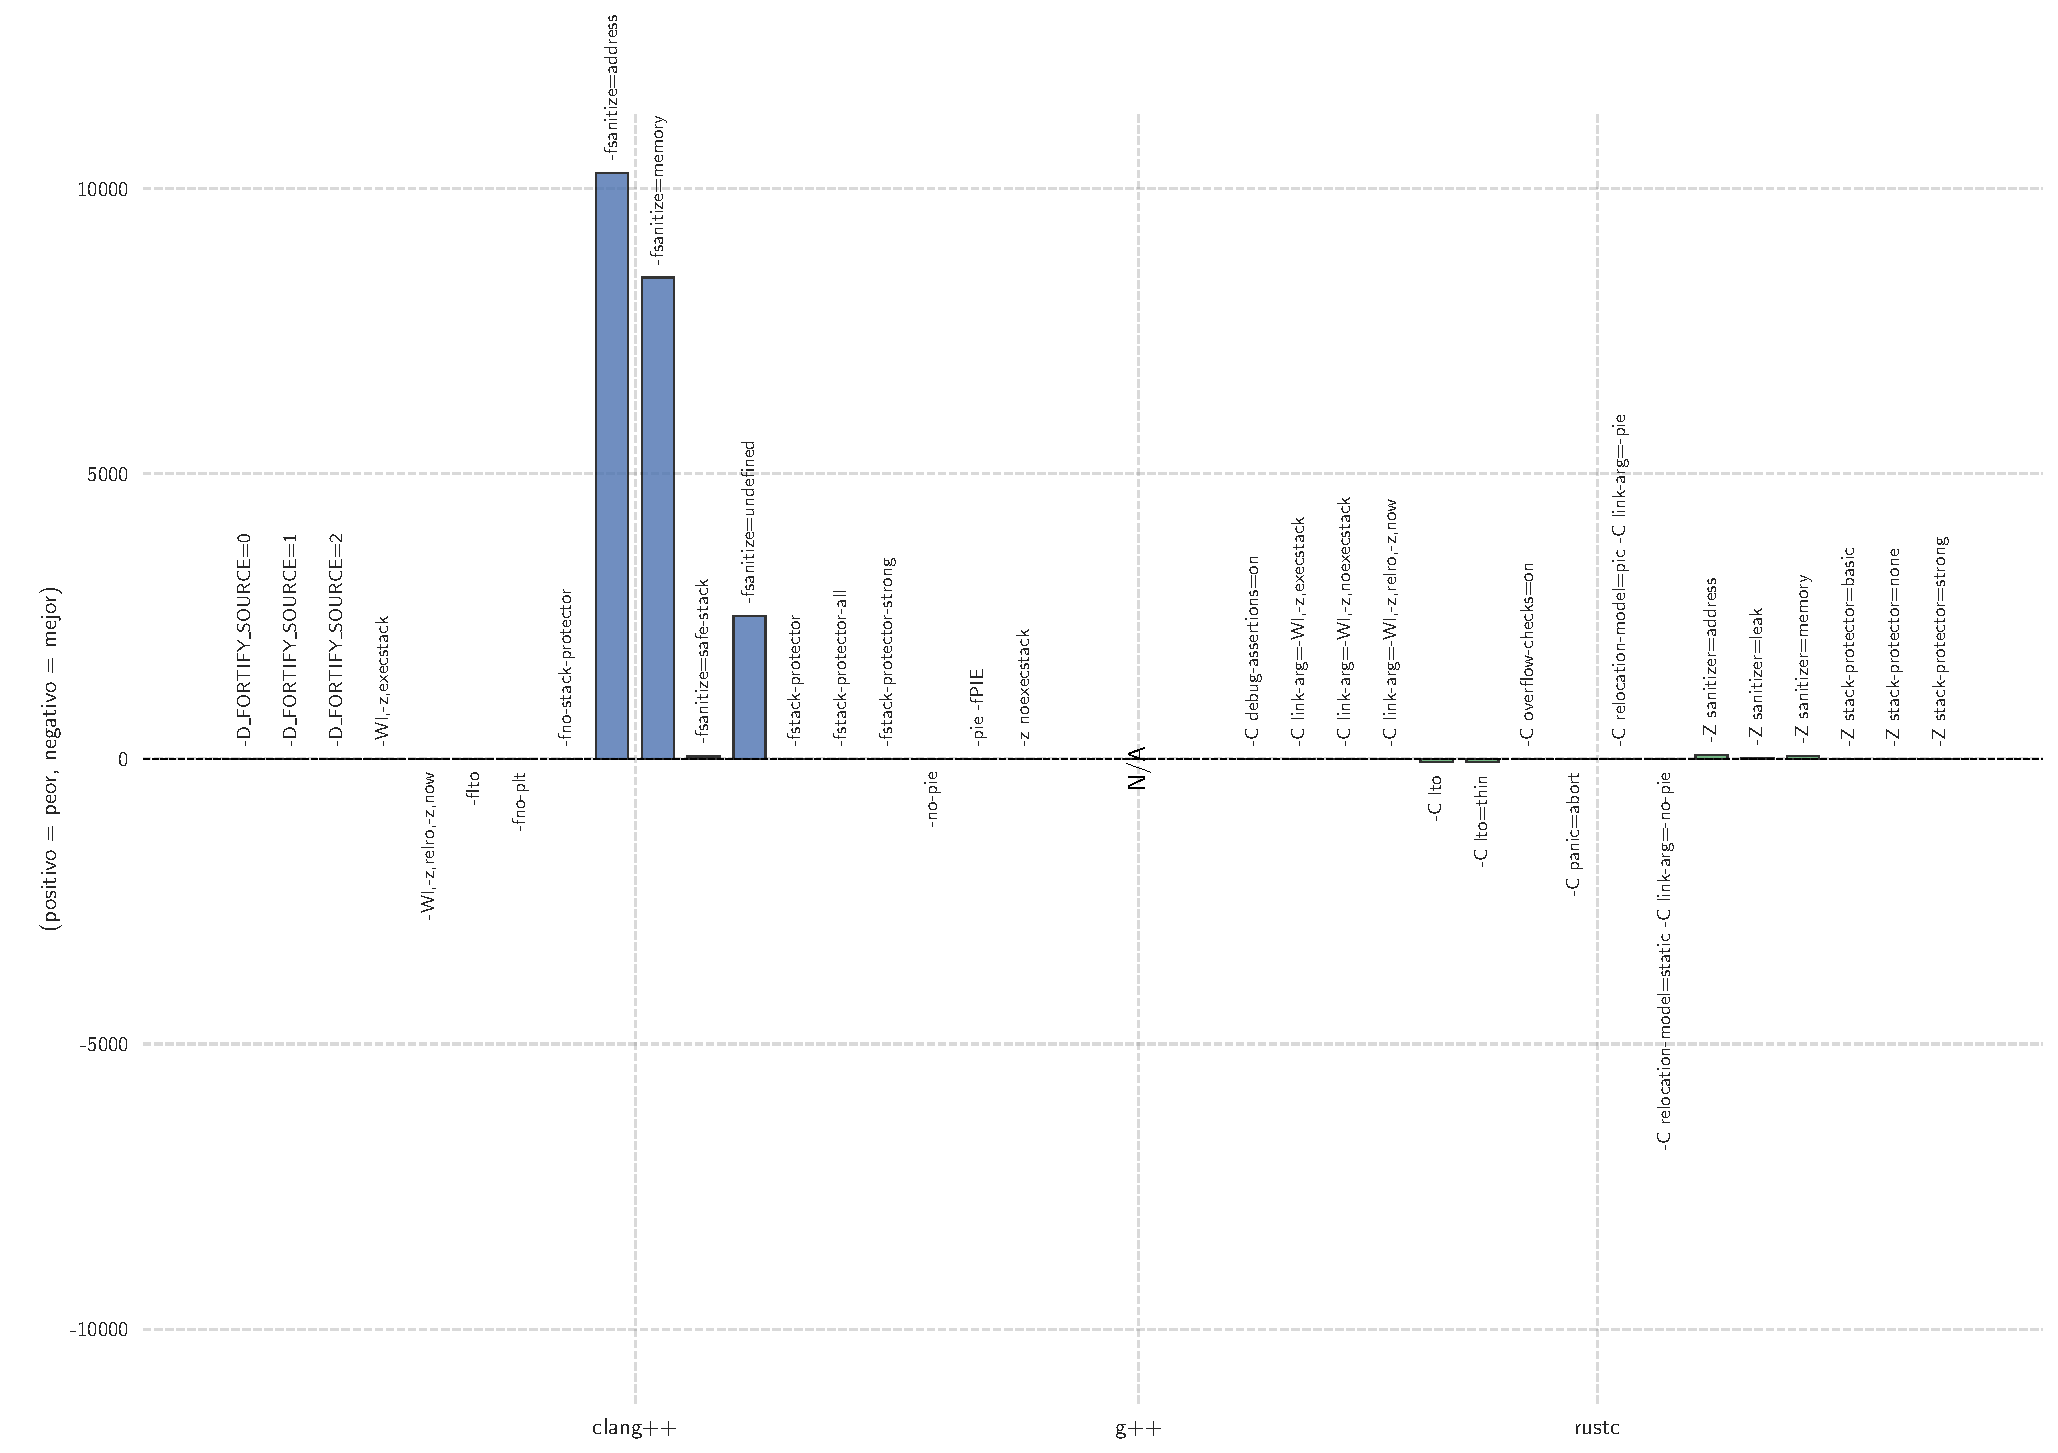
\includegraphics[width=\linewidth]{Gráficas/Gráficas_por_optimización_porcentual/-Oz/File_size_KB.pdf}
      \label{fig:Gráficas_gráficas_por_optimización_porcentual__oz_file_size_kb}
    }
  \end{minipage}
  \hfill
  \begin{minipage}{0.48\textwidth}
    \centering
    \subfloat[Funciones fortificadas (\%)]{
      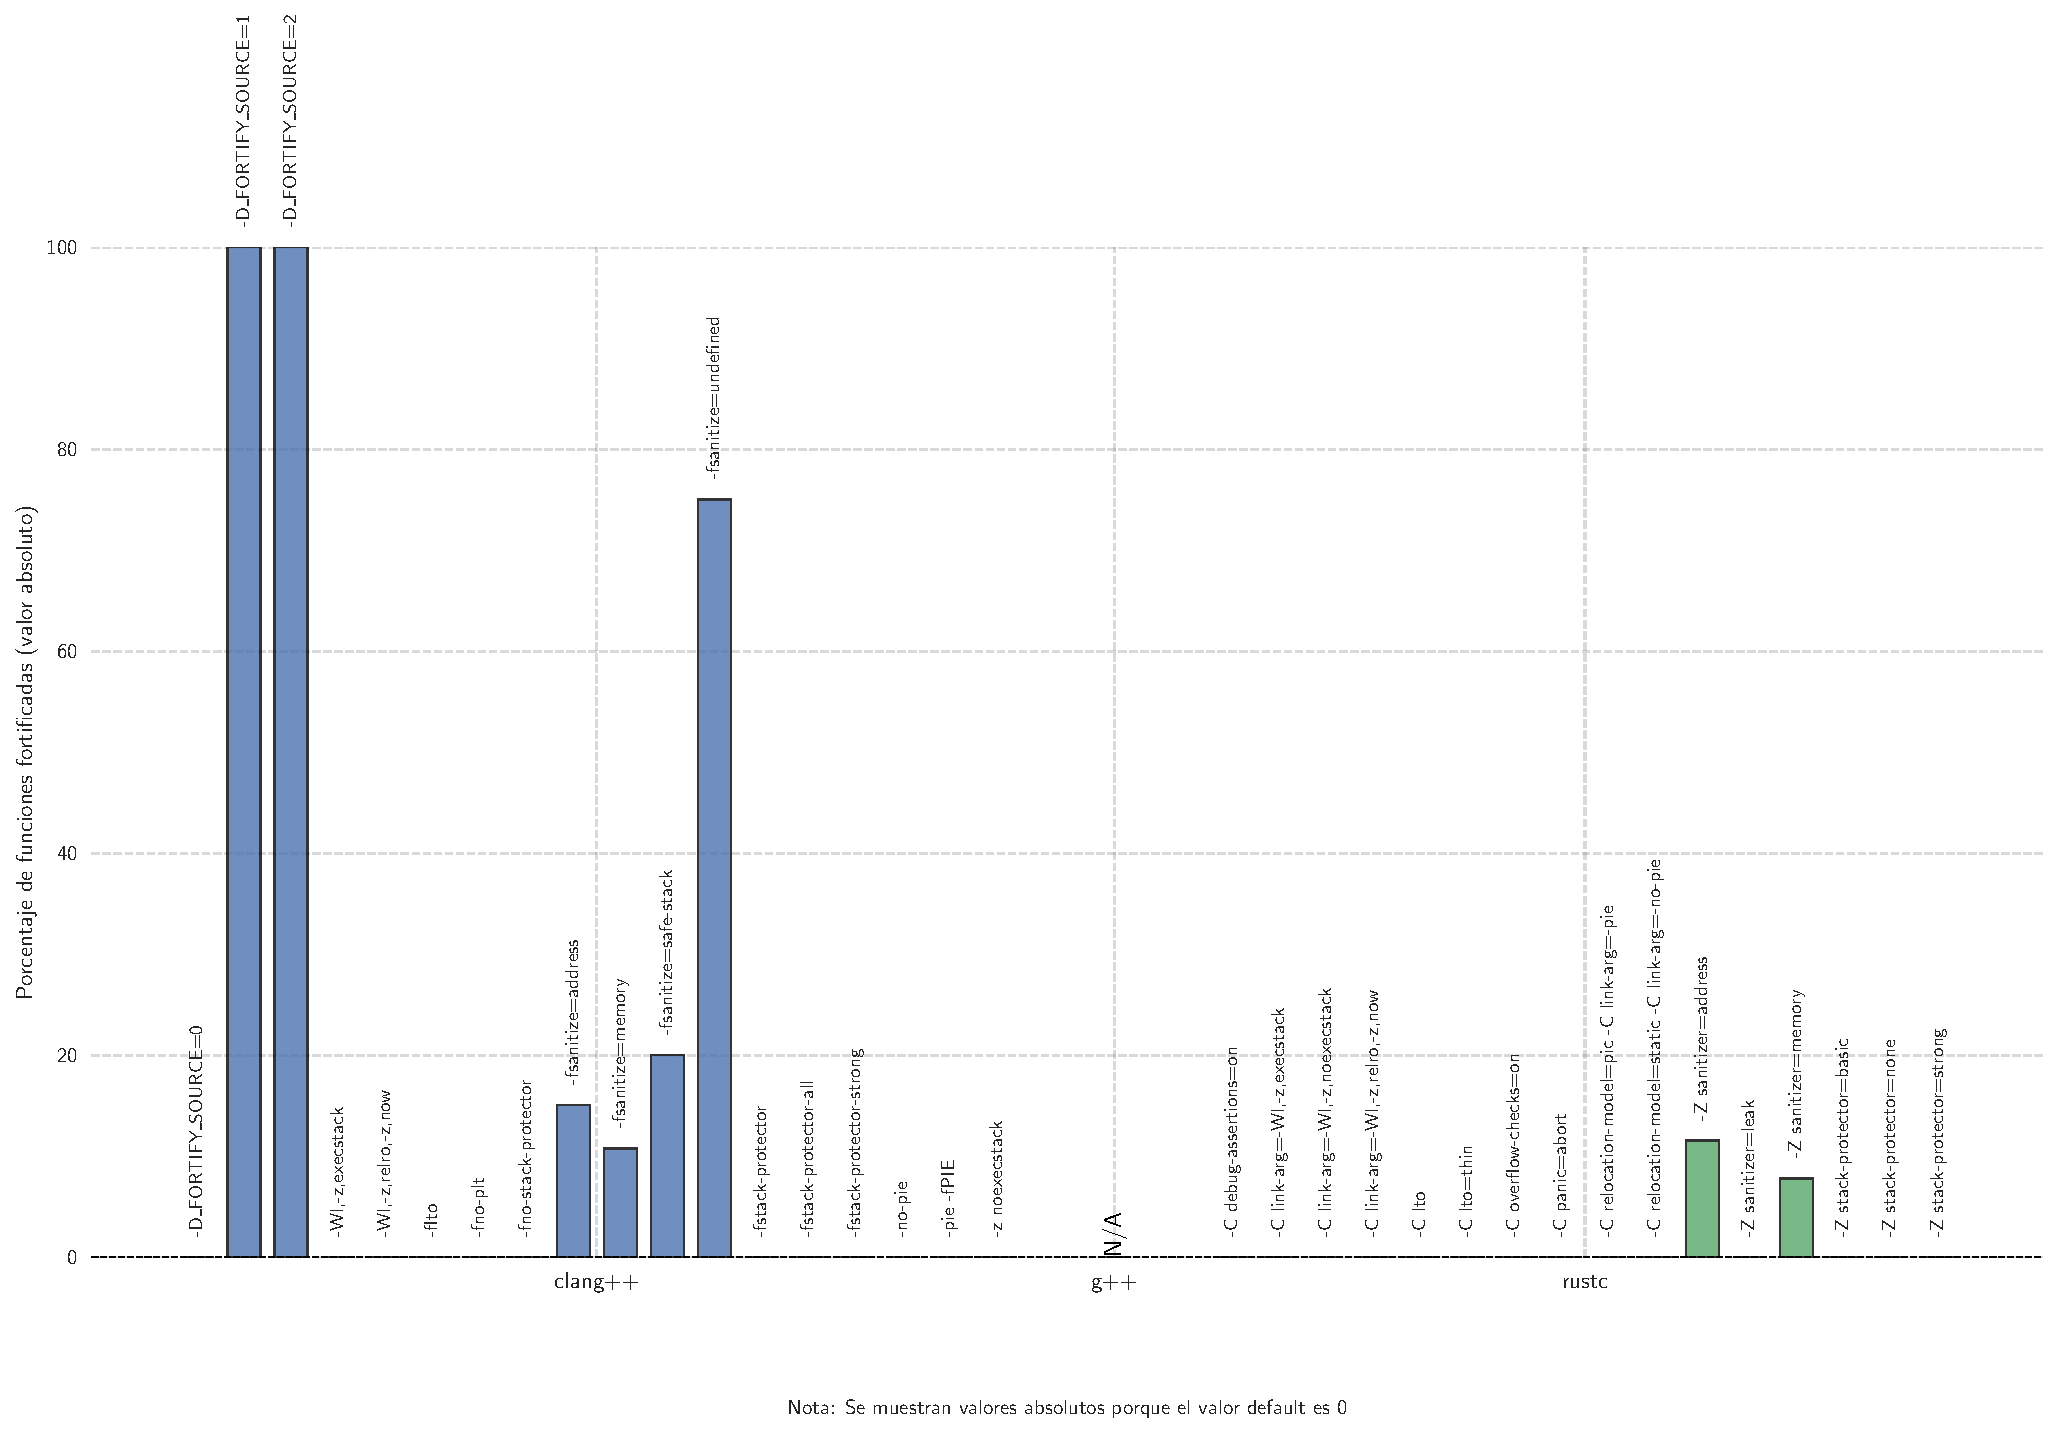
\includegraphics[width=\linewidth]{Gráficas/Gráficas_por_optimización_porcentual/-Oz/Fortified_Functions.pdf}
      \label{fig:Gráficas_gráficas_por_optimización_porcentual__oz_fortified_functions}
    }
  \end{minipage}


  \vspace{1cm}

  \begin{minipage}{0.48\textwidth}
    \centering
    \subfloat[Uso de memoria (KB)]{
      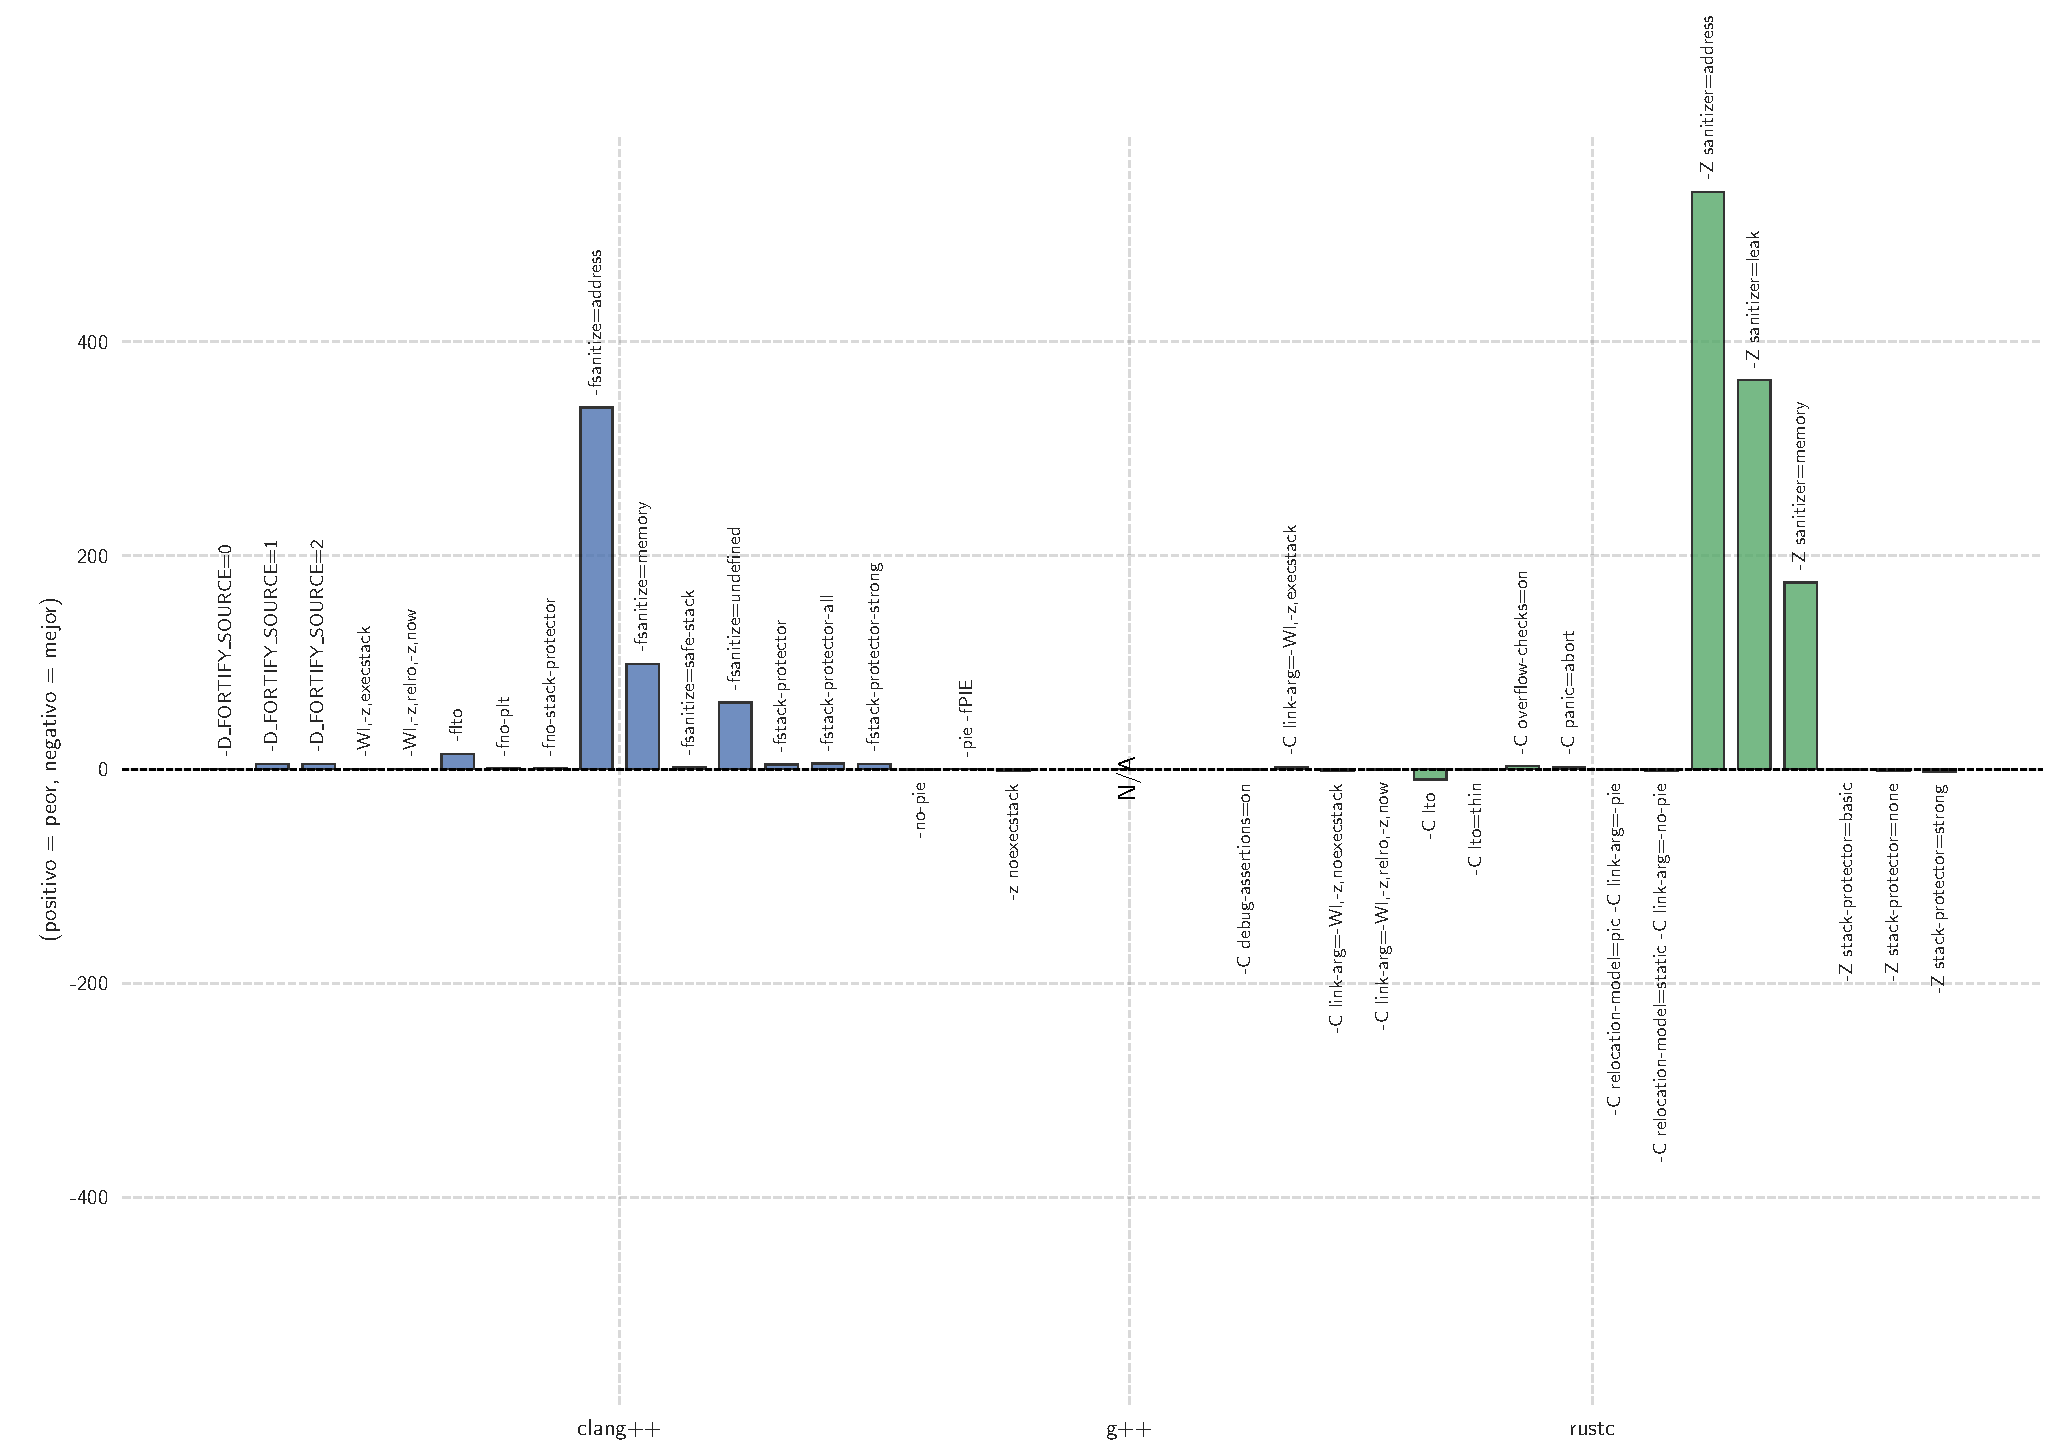
\includegraphics[width=\linewidth]{Gráficas/Gráficas_por_optimización_porcentual/-Oz/Memory_usage_KB.pdf}
      \label{fig:Gráficas_gráficas_por_optimización_porcentual__oz_memory_usage_kb}
    }
  \end{minipage}
  \hfill
  \begin{minipage}{0.48\textwidth}
    \centering
    \subfloat[Tiempo (ms)]{
      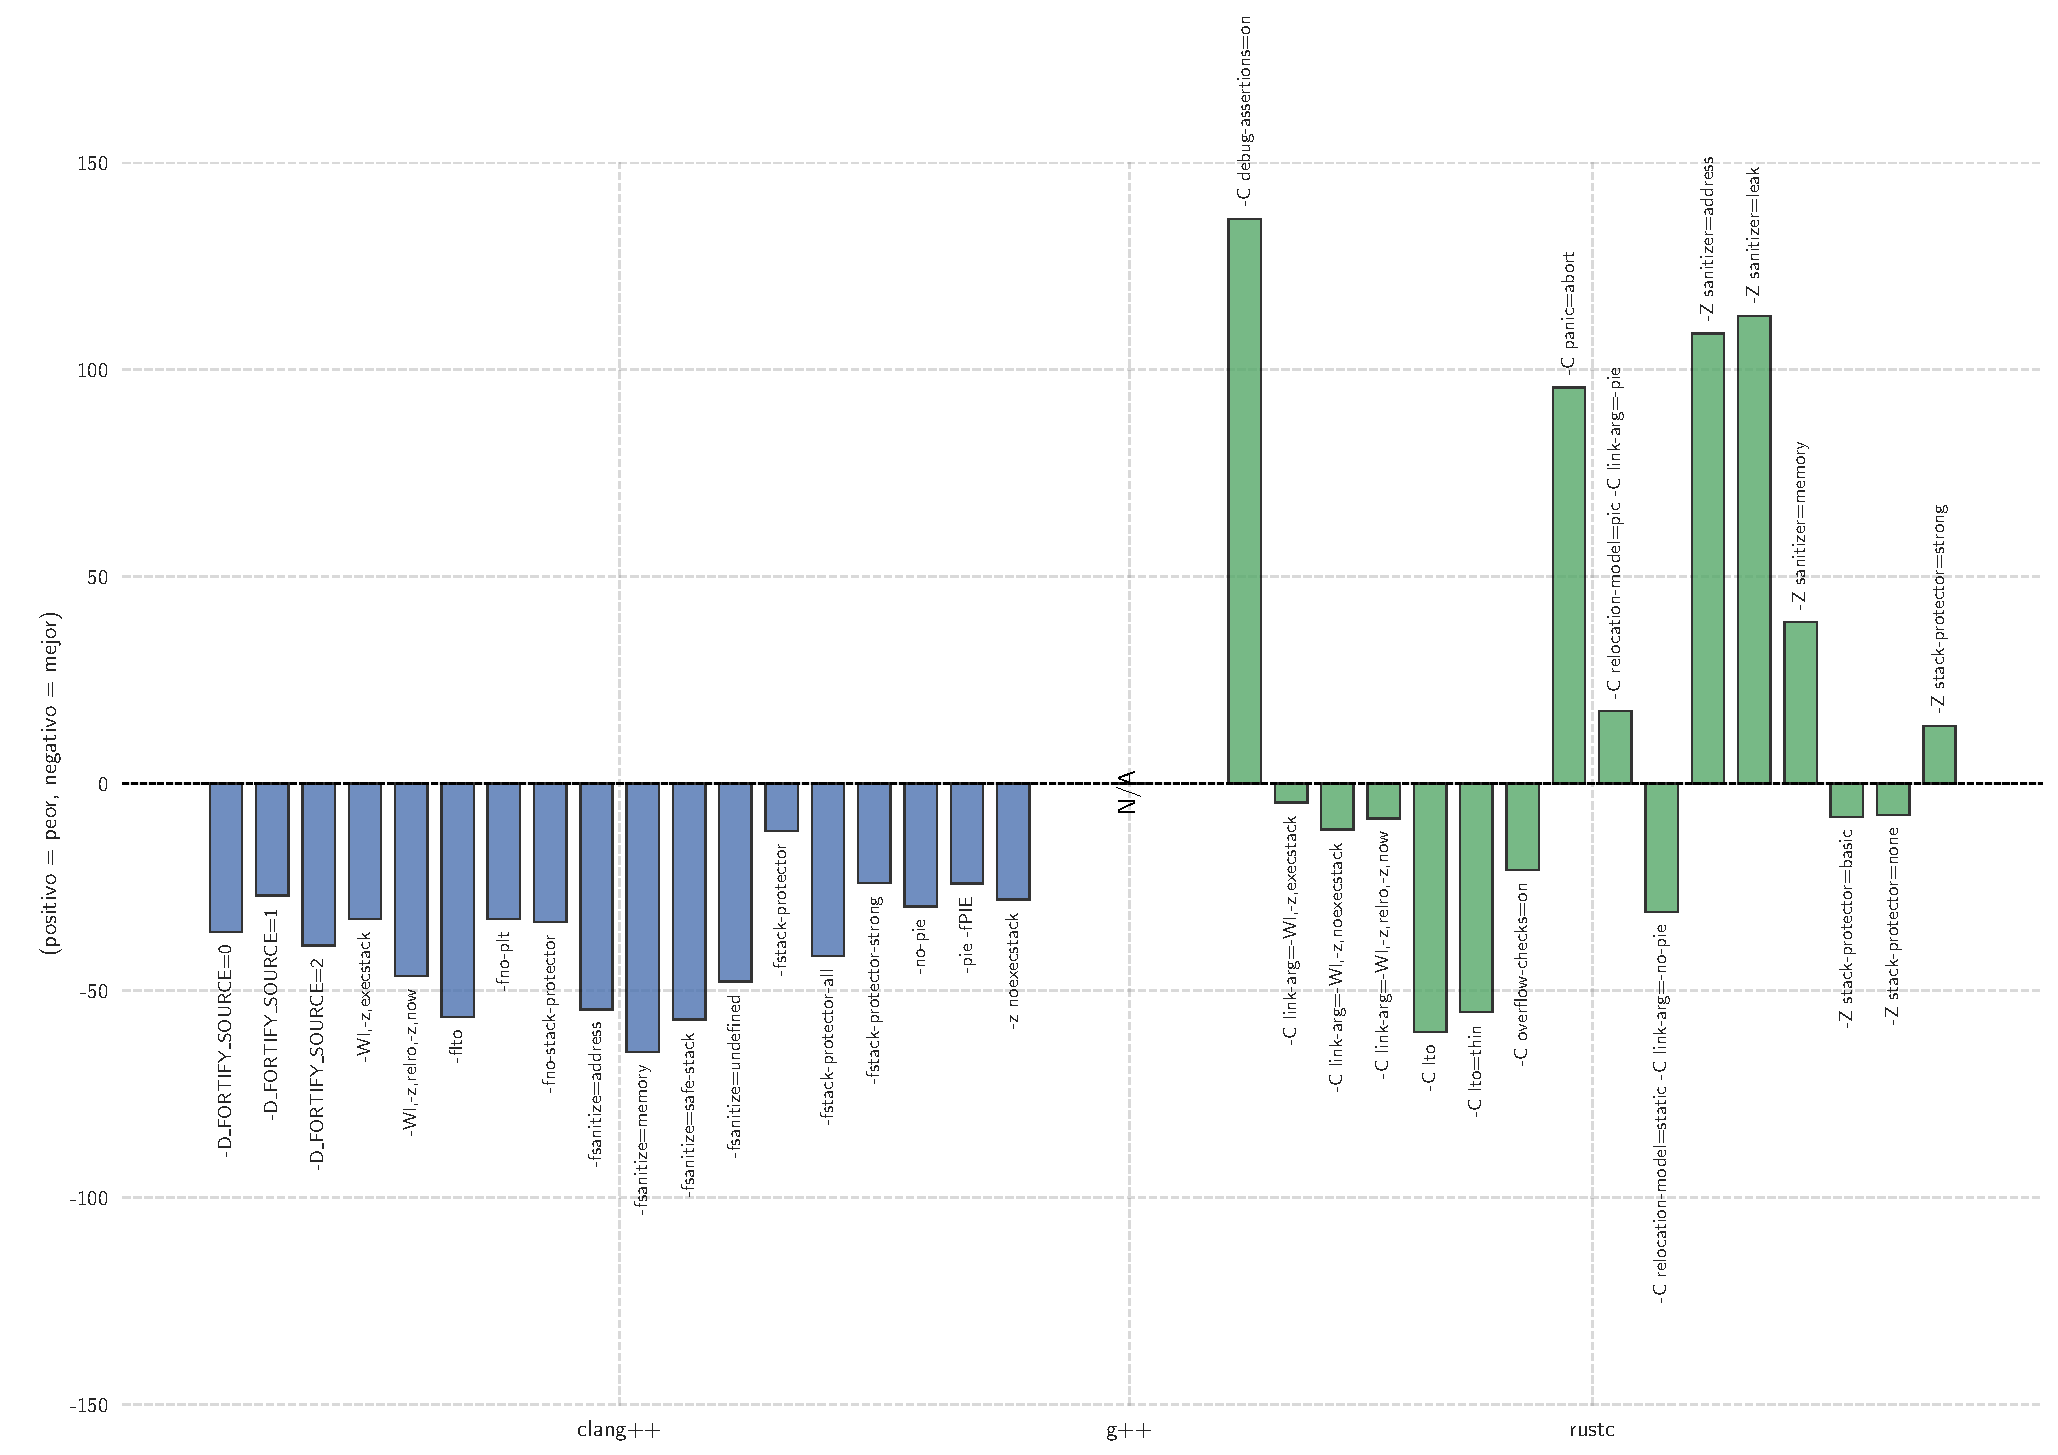
\includegraphics[width=\linewidth]{Gráficas/Gráficas_por_optimización_porcentual/-Oz/Time_ms.pdf}
      \label{fig:Gráficas_gráficas_por_optimización_porcentual__oz_time_ms}
    }
  \end{minipage}

\end{figure}
\newpage

\section*{Gráficas Por Medida Seguridad Porcentual}

% === Gráficas_por_medida_seguridad_porcentual/debug-assertions ===
\subsection*{Debug assertions}
\begin{figure}[htbp]
  \centering
  \caption{Resultados de compilación con optimización Debug assertions}
  \vspace{0.5cm}

  \begin{minipage}{0.48\textwidth}
    \centering
    \subfloat[Tamaño del archivo (KB) Porcentaje]{
      
\includegraphics[width=\linewidth]{Gráficas/Gráficas_por_medida_seguridad_porcentual/debug-assertions/File_size_KB_porcentaje.pdf}
      \label{fig:Gráficas_gráficas_por_medida_seguridad_porcentual_debug_assertions_file_size_kb_porcentaje}
    }
  \end{minipage}
  \hfill
  \begin{minipage}{0.48\textwidth}
    \centering
    \subfloat[Funciones fortificadas (\%) Porcentaje]{
      \includegraphics[width=\linewidth]{Gráficas/Gráficas_por_medida_seguridad_porcentual/debug-assertions/Fortified_Functions_porcentaje.pdf}
      \label{fig:Gráficas_gráficas_por_medida_seguridad_porcentual_debug_assertions_fortified_functions_porcentaje}
    }
  \end{minipage}


  \vspace{1cm}

  \begin{minipage}{0.48\textwidth}
    \centering
    \subfloat[Uso de memoria (KB) Porcentaje]{
      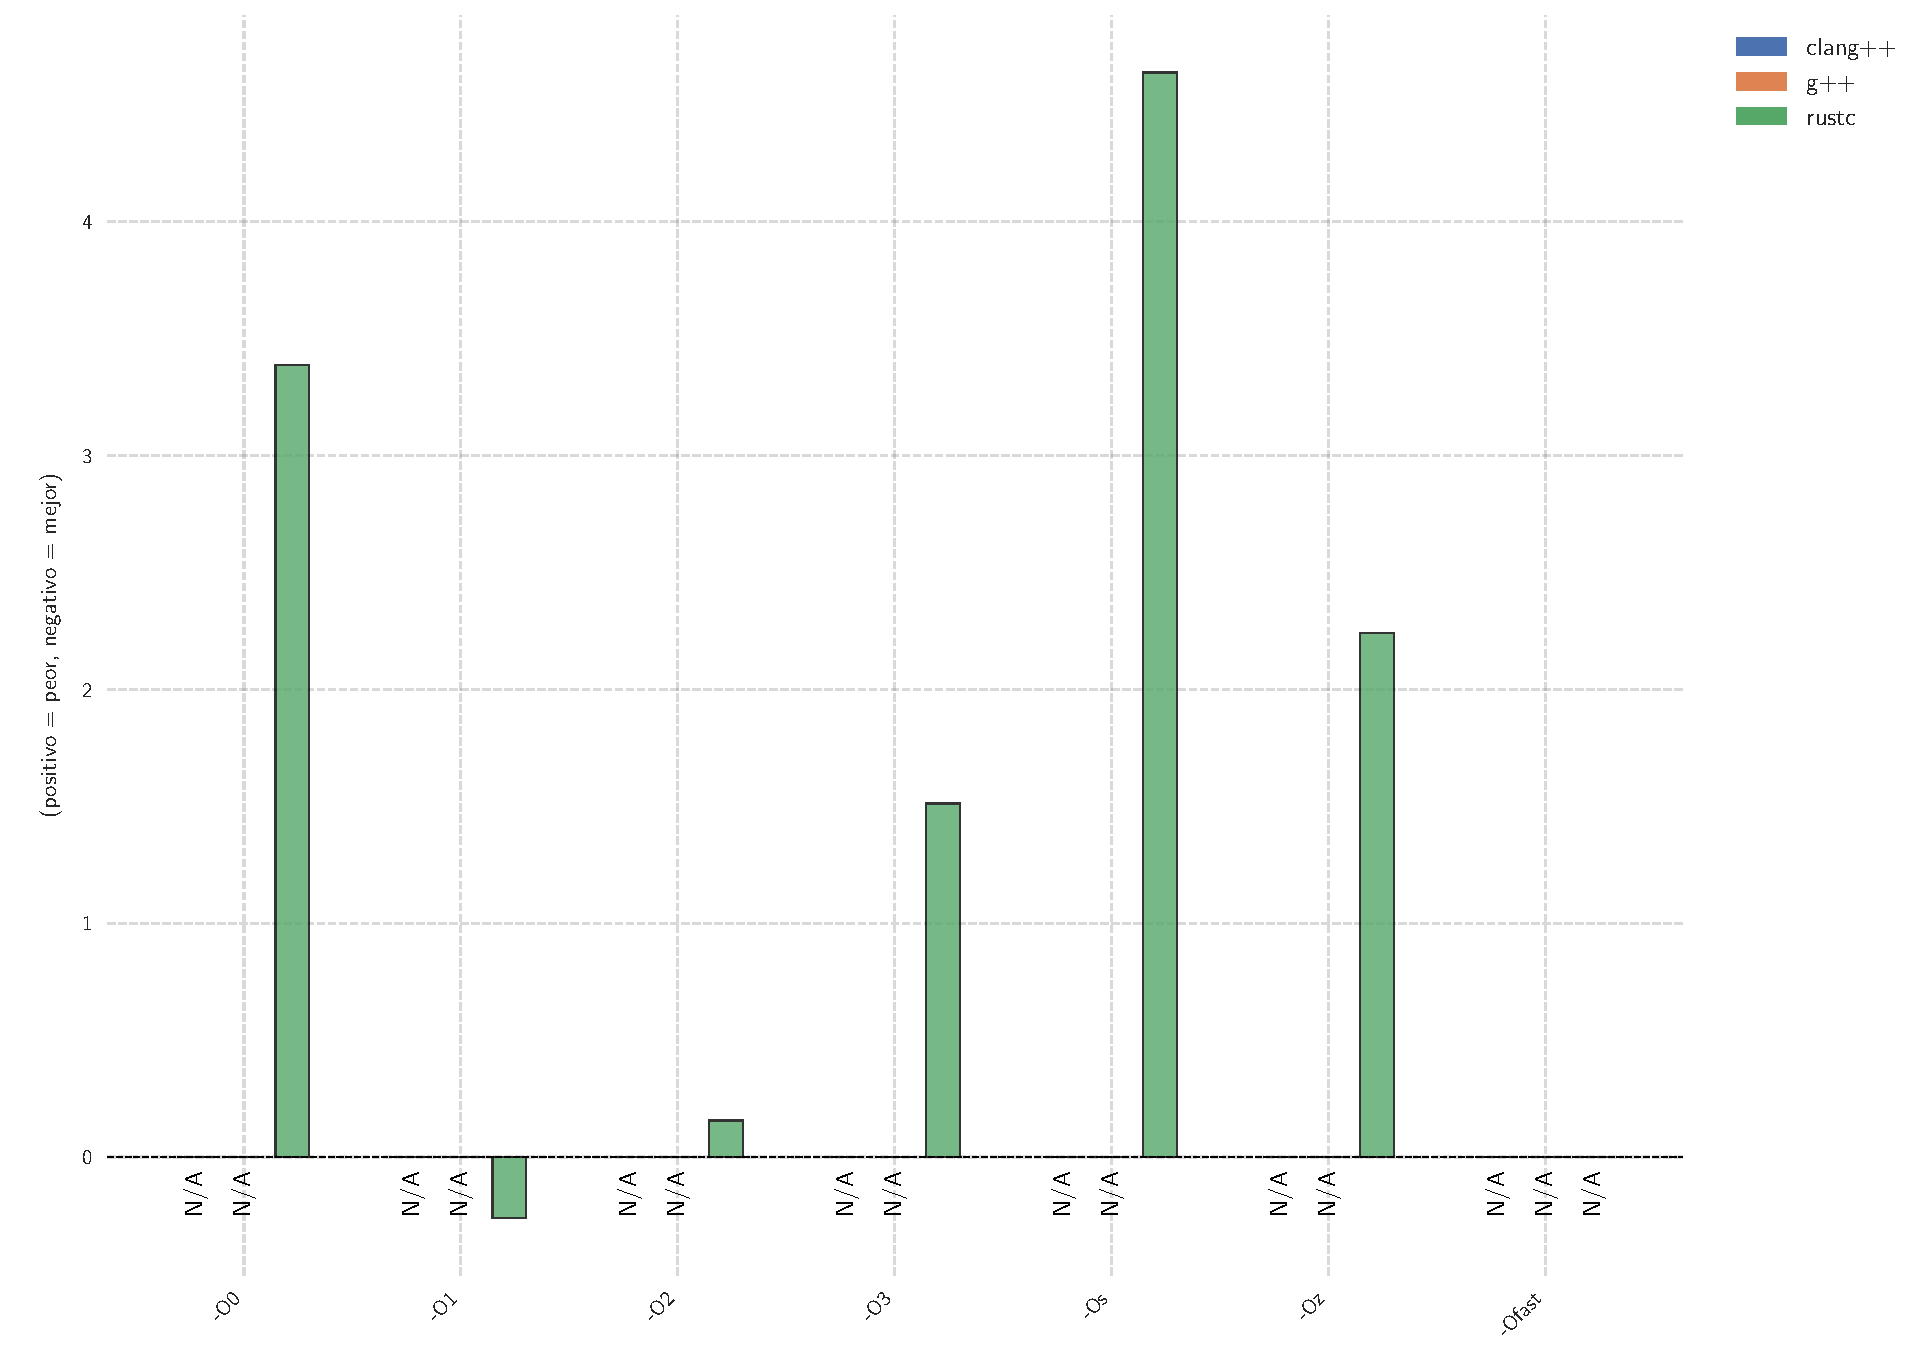
\includegraphics[width=\linewidth]{Gráficas/Gráficas_por_medida_seguridad_porcentual/debug-assertions/Memory_usage_KB_porcentaje.pdf}
      \label{fig:Gráficas_gráficas_por_medida_seguridad_porcentual_debug_assertions_memory_usage_kb_porcentaje}
    }
  \end{minipage}
  \hfill
  \begin{minipage}{0.48\textwidth}
    \centering
    \subfloat[Tiempo (ms) Porcentaje]{
      
\includegraphics[width=\linewidth]{Gráficas/Gráficas_por_medida_seguridad_porcentual/debug-assertions/Time_ms_porcentaje.pdf}
      \label{fig:Gráficas_gráficas_por_medida_seguridad_porcentual_debug_assertions_time_ms_porcentaje}
    }
  \end{minipage}

\end{figure}
\newpage

% === Gráficas_por_medida_seguridad_porcentual/execstack/disabled ===
\subsection*{Execstack / disabled}
\begin{figure}[htbp]
  \centering
  \caption{Resultados para Execstack (disabled)}
  \vspace{0.5cm}

  \begin{minipage}{0.48\textwidth}
    \centering
    \subfloat[Tamaño del archivo (KB) Porcentaje]{
      \includegraphics[width=\linewidth]{Gráficas/Gráficas_por_medida_seguridad_porcentual/execstack/disabled/File_size_KB_porcentaje.pdf}
      \label{fig:Gráficas_gráficas_por_medida_seguridad_porcentual_execstack_disabled_file_size_kb_porcentaje}
    }
  \end{minipage}
  \hfill
  \begin{minipage}{0.48\textwidth}
    \centering
    \subfloat[Funciones fortificadas (\%) Porcentaje]{
      \includegraphics[width=\linewidth]{Gráficas/Gráficas_por_medida_seguridad_porcentual/execstack/disabled/Fortified_Functions_porcentaje.pdf}
      \label{fig:Gráficas_gráficas_por_medida_seguridad_porcentual_execstack_disabled_fortified_functions_porcentaje}
    }
  \end{minipage}


  \vspace{1cm}

  \begin{minipage}{0.48\textwidth}
    \centering
    \subfloat[Uso de memoria (KB) Porcentaje]{
      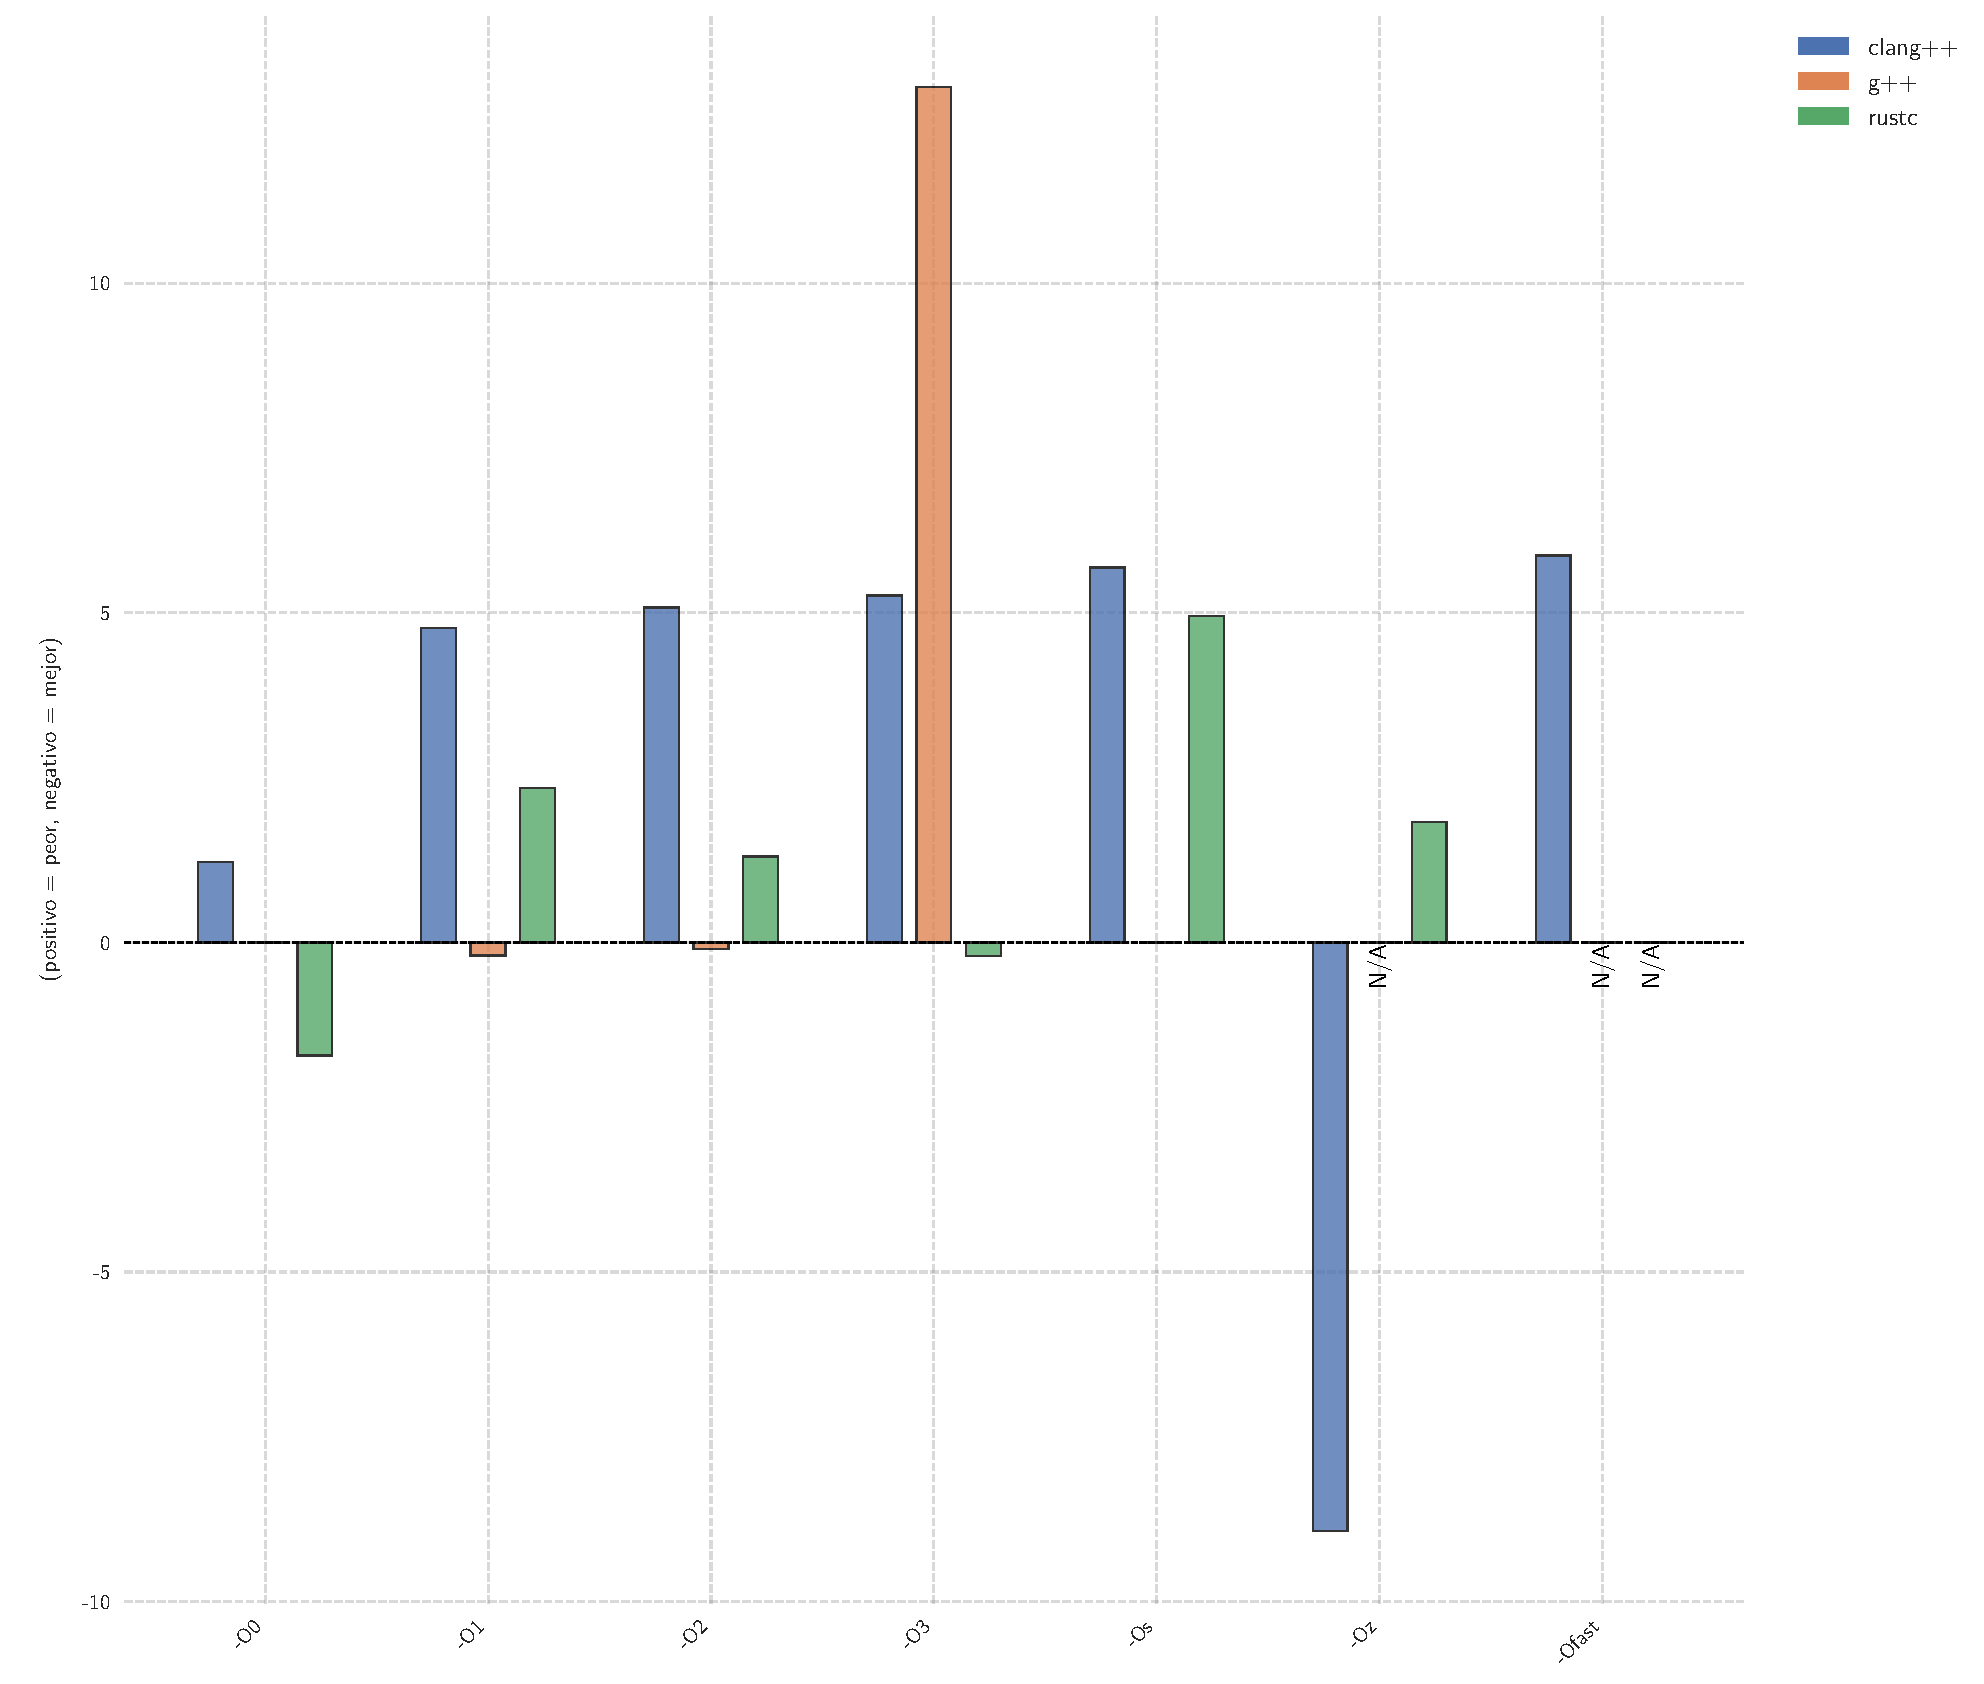
\includegraphics[width=\linewidth]{Gráficas/Gráficas_por_medida_seguridad_porcentual/execstack/disabled/Memory_usage_KB_porcentaje.pdf}
      \label{fig:Gráficas_gráficas_por_medida_seguridad_porcentual_execstack_disabled_memory_usage_kb_porcentaje}
    }
  \end{minipage}
  \hfill
  \begin{minipage}{0.48\textwidth}
    \centering
    \subfloat[Tiempo (ms) Porcentaje]{
      
\includegraphics[width=\linewidth]{Gráficas/Gráficas_por_medida_seguridad_porcentual/execstack/disabled/Time_ms_porcentaje.pdf}
      \label{fig:Gráficas_gráficas_por_medida_seguridad_porcentual_execstack_disabled_time_ms_porcentaje}
    }
  \end{minipage}

\end{figure}
\newpage

% === Gráficas_por_medida_seguridad_porcentual/execstack/enabled ===
\subsection*{Execstack / enabled}
\begin{figure}[htbp]
  \centering
  \caption{Resultados para Execstack (enabled)}
  \vspace{0.5cm}

  \begin{minipage}{0.48\textwidth}
    \centering
    \subfloat[Tamaño del archivo (KB) Porcentaje]{
      \includegraphics[width=\linewidth]{Gráficas/Gráficas_por_medida_seguridad_porcentual/execstack/enabled/File_size_KB_porcentaje.pdf}
      \label{fig:Gráficas_gráficas_por_medida_seguridad_porcentual_execstack_enabled_file_size_kb_porcentaje}
    }
  \end{minipage}
  \hfill
  \begin{minipage}{0.48\textwidth}
    \centering
    \subfloat[Funciones fortificadas (\%) Porcentaje]{
      \includegraphics[width=\linewidth]{Gráficas/Gráficas_por_medida_seguridad_porcentual/execstack/enabled/Fortified_Functions_porcentaje.pdf}
      \label{fig:Gráficas_gráficas_por_medida_seguridad_porcentual_execstack_enabled_fortified_functions_porcentaje}
    }
  \end{minipage}


  \vspace{1cm}

  \begin{minipage}{0.48\textwidth}
    \centering
    \subfloat[Uso de memoria (KB) Porcentaje]{
      
\includegraphics[width=\linewidth]{Gráficas/Gráficas_por_medida_seguridad_porcentual/execstack/enabled/Memory_usage_KB_porcentaje.pdf}
      \label{fig:Gráficas_gráficas_por_medida_seguridad_porcentual_execstack_enabled_memory_usage_kb_porcentaje}
    }
  \end{minipage}
  \hfill
  \begin{minipage}{0.48\textwidth}
    \centering
    \subfloat[Tiempo (ms) Porcentaje]{
      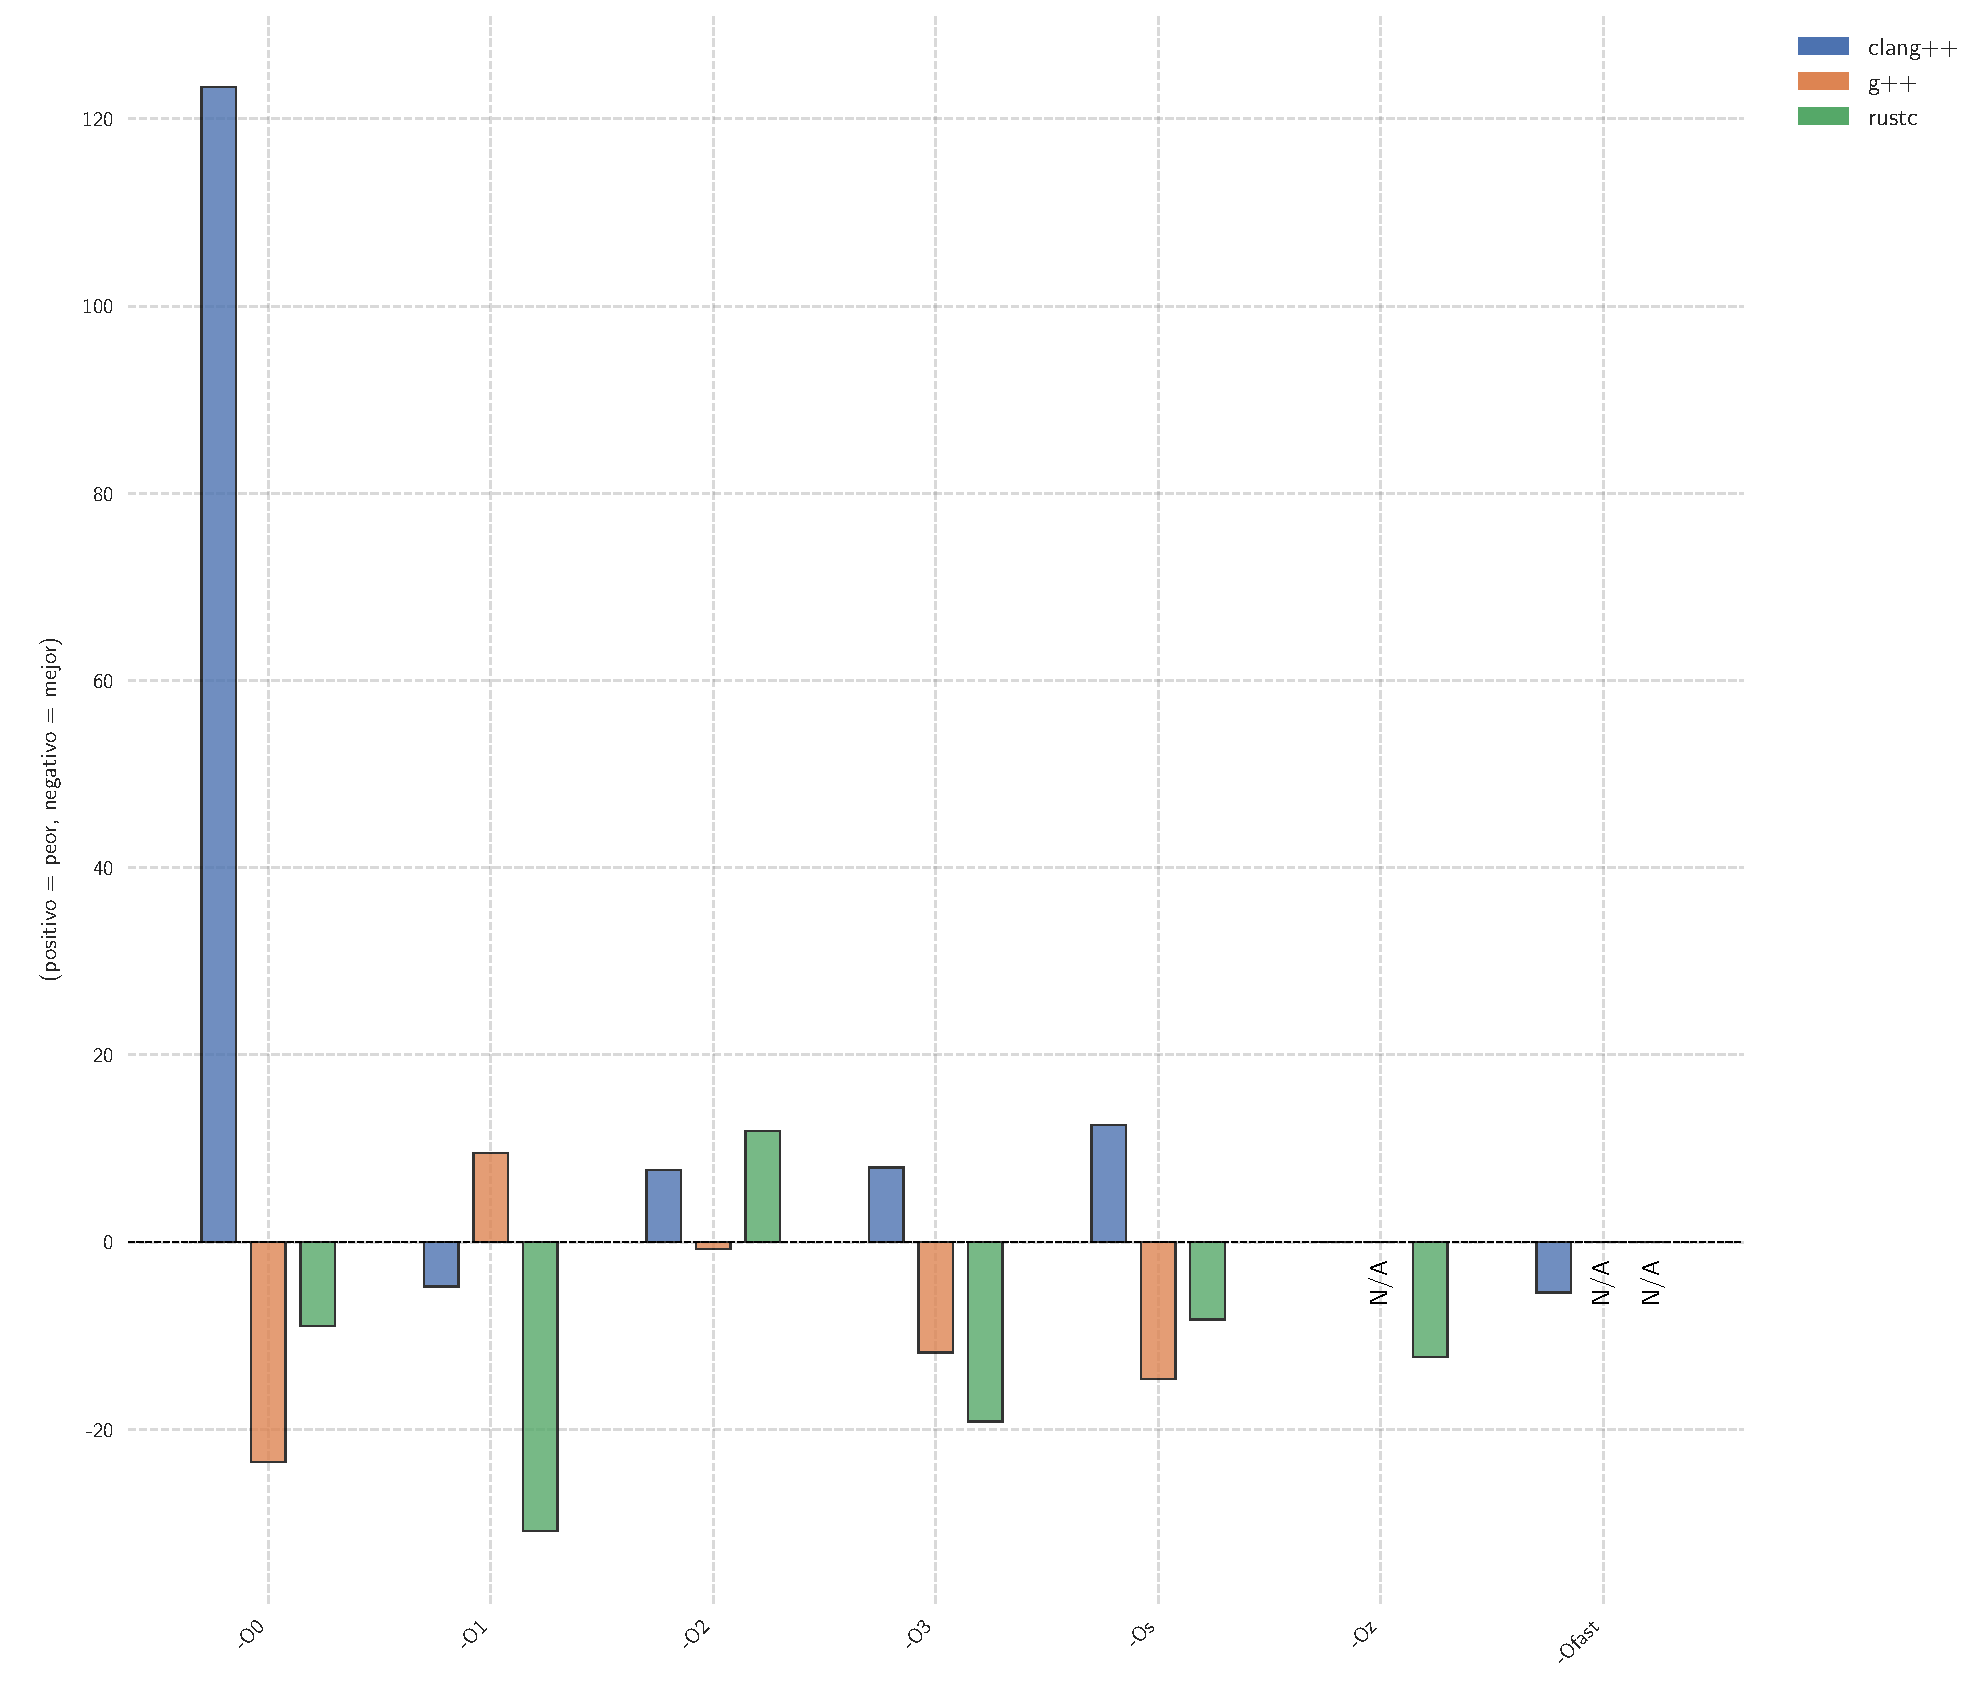
\includegraphics[width=\linewidth]{Gráficas/Gráficas_por_medida_seguridad_porcentual/execstack/enabled/Time_ms_porcentaje.pdf}
      \label{fig:Gráficas_gráficas_por_medida_seguridad_porcentual_execstack_enabled_time_ms_porcentaje}
    }
  \end{minipage}

\end{figure}
\newpage

% === Gráficas_por_medida_seguridad_porcentual/fortify-source/disabled ===
\subsection*{Fortify source / disabled}
\begin{figure}[htbp]
  \centering
  \caption{Resultados para Fortify source (disabled)}
  \vspace{0.5cm}

  \begin{minipage}{0.48\textwidth}
    \centering
    \subfloat[Tamaño del archivo (KB) Porcentaje]{
      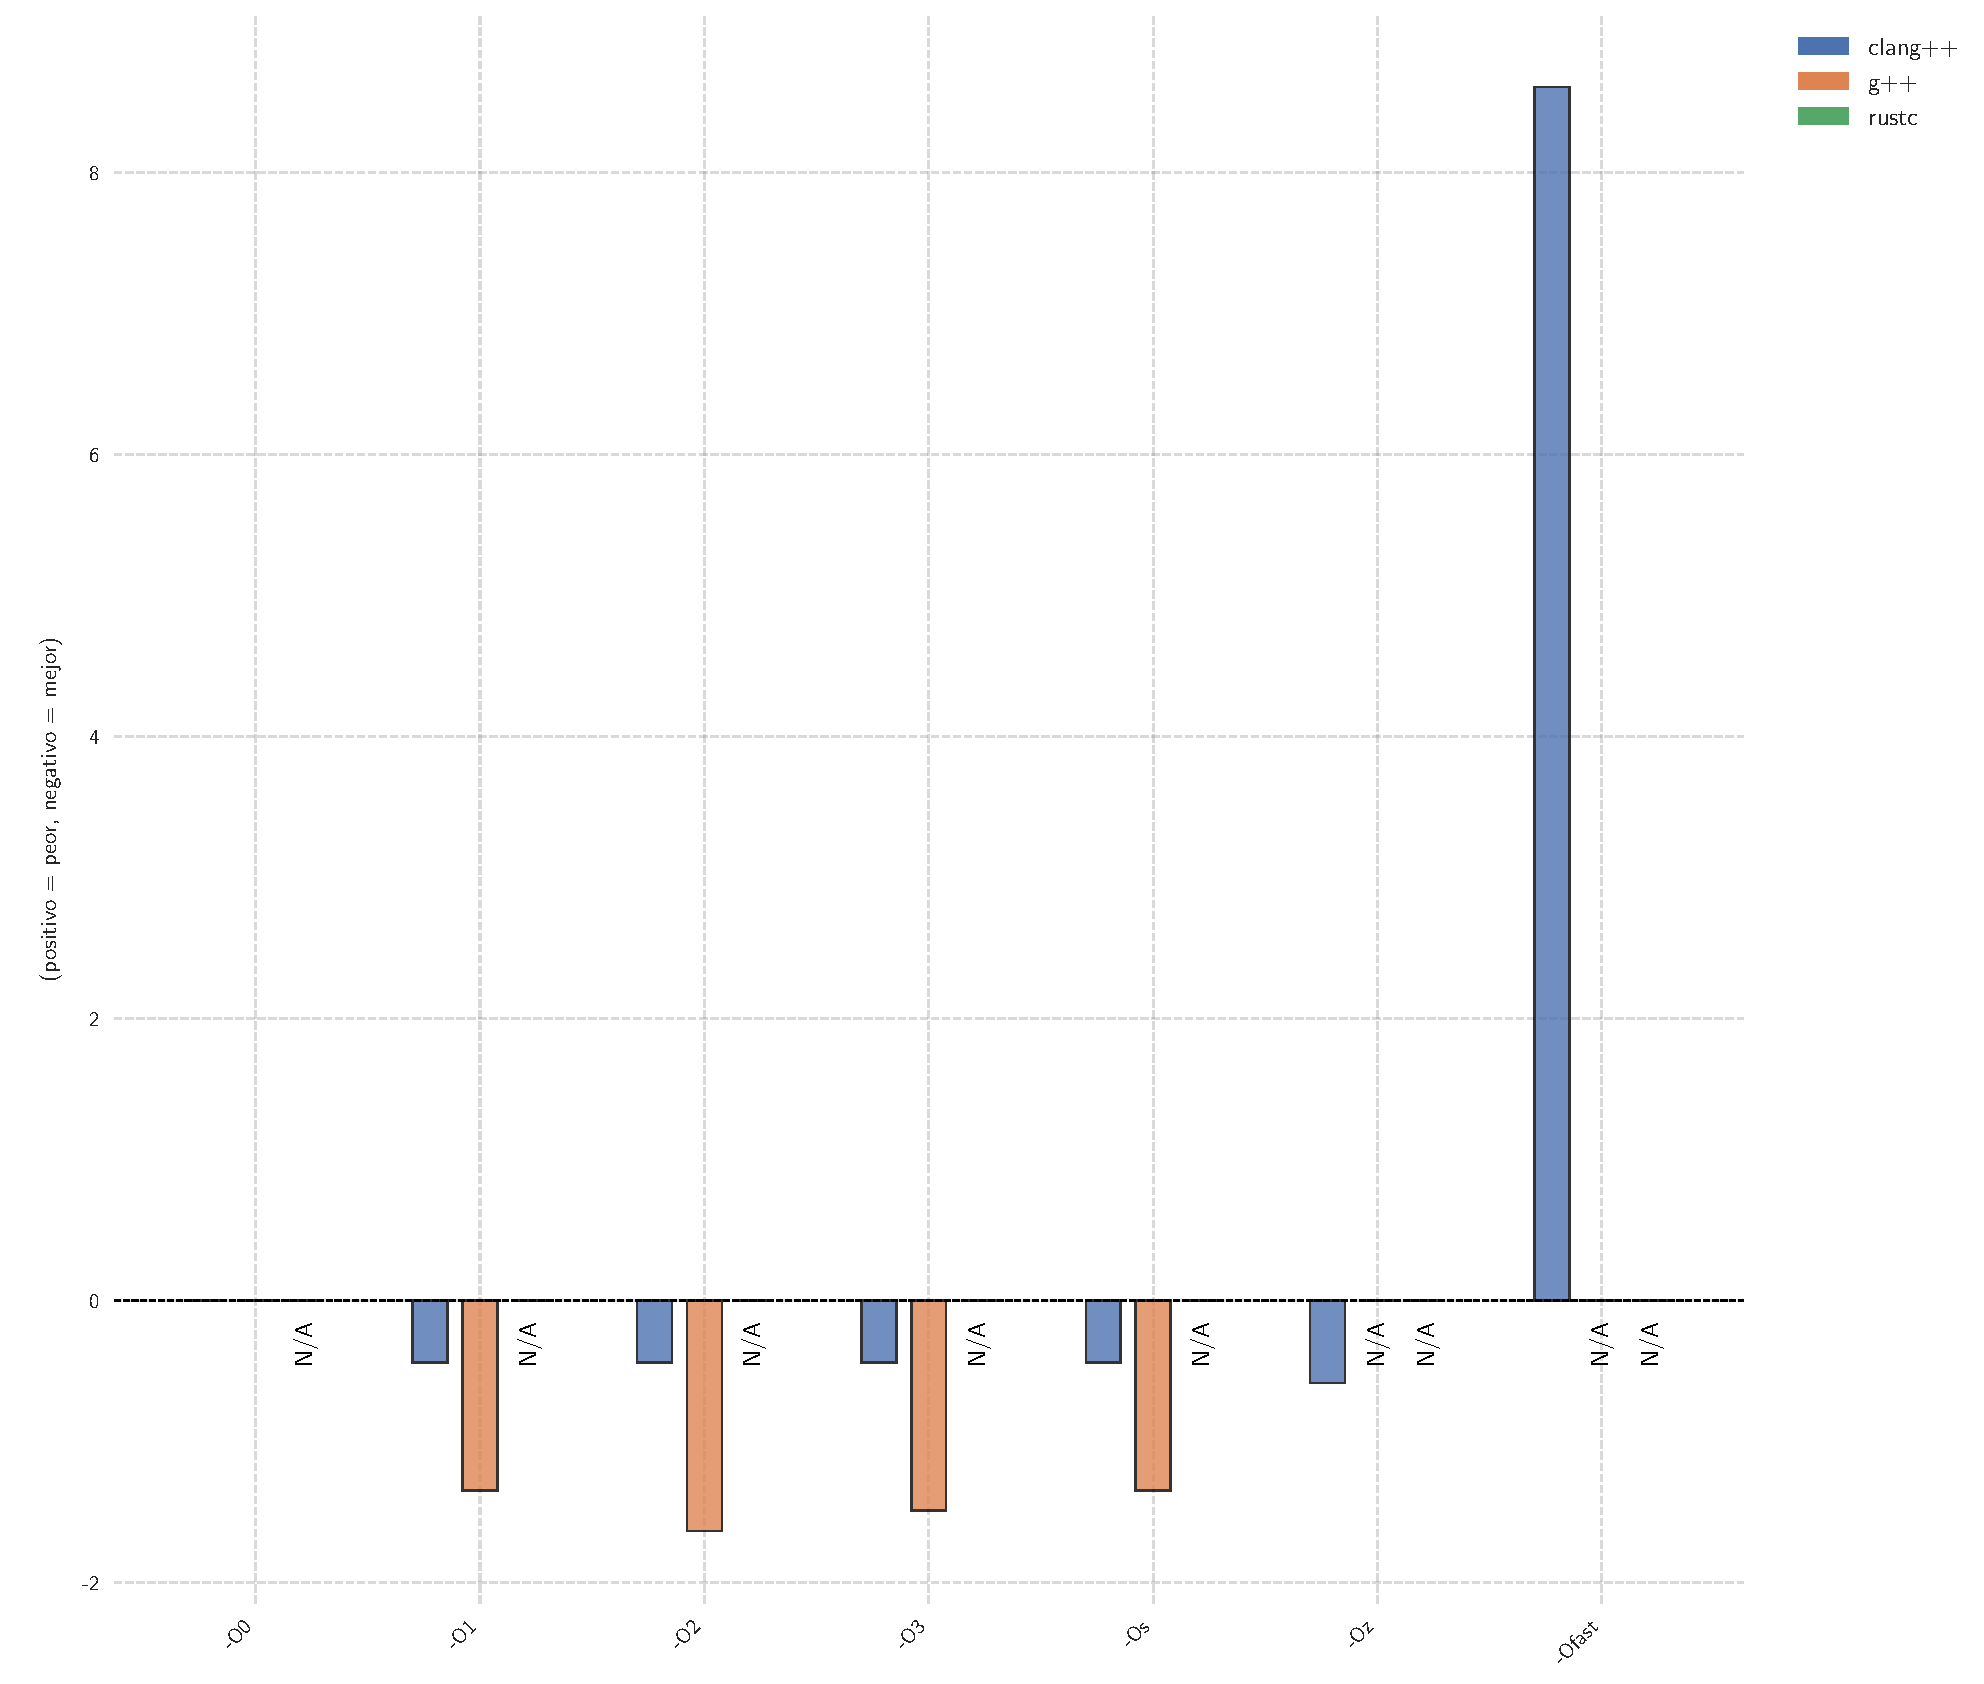
\includegraphics[width=\linewidth]{Gráficas/Gráficas_por_medida_seguridad_porcentual/fortify-source/disabled/File_size_KB_porcentaje.pdf}
      \label{fig:Gráficas_gráficas_por_medida_seguridad_porcentual_fortify_source_disabled_file_size_kb_porcentaje}
    }
  \end{minipage}
  \hfill
  \begin{minipage}{0.48\textwidth}
    \centering
    \subfloat[Funciones fortificadas (\%) Porcentaje]{
      \includegraphics[width=\linewidth]{Gráficas/Gráficas_por_medida_seguridad_porcentual/fortify-source/disabled/Fortified_Functions_porcentaje.pdf}
      \label{fig:Gráficas_gráficas_por_medida_seguridad_porcentual_fortify_source_disabled_fortified_functions_porcentaje}
    }
  \end{minipage}


  \vspace{1cm}

  \begin{minipage}{0.48\textwidth}
    \centering
    \subfloat[Uso de memoria (KB) Porcentaje]{
      
\includegraphics[width=\linewidth]{Gráficas/Gráficas_por_medida_seguridad_porcentual/fortify-source/disabled/Memory_usage_KB_porcentaje.pdf}
      \label{fig:Gráficas_gráficas_por_medida_seguridad_porcentual_fortify_source_disabled_memory_usage_kb_porcentaje}
    }
  \end{minipage}
  \hfill
  \begin{minipage}{0.48\textwidth}
    \centering
    \subfloat[Tiempo (ms) Porcentaje]{
      
\includegraphics[width=\linewidth]{Gráficas/Gráficas_por_medida_seguridad_porcentual/fortify-source/disabled/Time_ms_porcentaje.pdf}
      \label{fig:Gráficas_gráficas_por_medida_seguridad_porcentual_fortify_source_disabled_time_ms_porcentaje}
    }
  \end{minipage}

\end{figure}
\newpage

% === Gráficas_por_medida_seguridad_porcentual/fortify-source/level-1 ===
\subsection*{Fortify source / level-1}
\begin{figure}[htbp]
  \centering
  \caption{Resultados para Fortify source (level-1)}
  \vspace{0.5cm}

  \begin{minipage}{0.48\textwidth}
    \centering
    \subfloat[Tamaño del archivo (KB) Porcentaje]{
      
\includegraphics[width=\linewidth]{Gráficas/Gráficas_por_medida_seguridad_porcentual/fortify-source/level-1/File_size_KB_porcentaje.pdf}
      \label{fig:Gráficas_gráficas_por_medida_seguridad_porcentual_fortify_source_level_1_file_size_kb_porcentaje}
    }
  \end{minipage}
  \hfill
  \begin{minipage}{0.48\textwidth}
    \centering
    \subfloat[Funciones fortificadas (\%) Porcentaje]{
      \includegraphics[width=\linewidth]{Gráficas/Gráficas_por_medida_seguridad_porcentual/fortify-source/level-1/Fortified_Functions_porcentaje.pdf}
      \label{fig:Gráficas_gráficas_por_medida_seguridad_porcentual_fortify_source_level_1_fortified_functions_porcentaje}
    }
  \end{minipage}


  \vspace{1cm}

  \begin{minipage}{0.48\textwidth}
    \centering
    \subfloat[Uso de memoria (KB) Porcentaje]{
      
\includegraphics[width=\linewidth]{Gráficas/Gráficas_por_medida_seguridad_porcentual/fortify-source/level-1/Memory_usage_KB_porcentaje.pdf}
      \label{fig:Gráficas_gráficas_por_medida_seguridad_porcentual_fortify_source_level_1_memory_usage_kb_porcentaje}
    }
  \end{minipage}
  \hfill
  \begin{minipage}{0.48\textwidth}
    \centering
    \subfloat[Tiempo (ms) Porcentaje]{
      
\includegraphics[width=\linewidth]{Gráficas/Gráficas_por_medida_seguridad_porcentual/fortify-source/level-1/Time_ms_porcentaje.pdf}
      \label{fig:Gráficas_gráficas_por_medida_seguridad_porcentual_fortify_source_level_1_time_ms_porcentaje}
    }
  \end{minipage}

\end{figure}
\newpage

% === Gráficas_por_medida_seguridad_porcentual/fortify-source/level-2 ===
\subsection*{Fortify source / level-2}
\begin{figure}[htbp]
  \centering
  \caption{Resultados para Fortify source (level-2)}
  \vspace{0.5cm}

  \begin{minipage}{0.48\textwidth}
    \centering
    \subfloat[Tamaño del archivo (KB) Porcentaje]{
      
\includegraphics[width=\linewidth]{Gráficas/Gráficas_por_medida_seguridad_porcentual/fortify-source/level-2/File_size_KB_porcentaje.pdf}
      \label{fig:Gráficas_gráficas_por_medida_seguridad_porcentual_fortify_source_level_2_file_size_kb_porcentaje}
    }
  \end{minipage}
  \hfill
  \begin{minipage}{0.48\textwidth}
    \centering
    \subfloat[Funciones fortificadas (\%) Porcentaje]{
      \includegraphics[width=\linewidth]{Gráficas/Gráficas_por_medida_seguridad_porcentual/fortify-source/level-2/Fortified_Functions_porcentaje.pdf}
      \label{fig:Gráficas_gráficas_por_medida_seguridad_porcentual_fortify_source_level_2_fortified_functions_porcentaje}
    }
  \end{minipage}


  \vspace{1cm}

  \begin{minipage}{0.48\textwidth}
    \centering
    \subfloat[Uso de memoria (KB) Porcentaje]{
      
\includegraphics[width=\linewidth]{Gráficas/Gráficas_por_medida_seguridad_porcentual/fortify-source/level-2/Memory_usage_KB_porcentaje.pdf}
      \label{fig:Gráficas_gráficas_por_medida_seguridad_porcentual_fortify_source_level_2_memory_usage_kb_porcentaje}
    }
  \end{minipage}
  \hfill
  \begin{minipage}{0.48\textwidth}
    \centering
    \subfloat[Tiempo (ms) Porcentaje]{
      
\includegraphics[width=\linewidth]{Gráficas/Gráficas_por_medida_seguridad_porcentual/fortify-source/level-2/Time_ms_porcentaje.pdf}
      \label{fig:Gráficas_gráficas_por_medida_seguridad_porcentual_fortify_source_level_2_time_ms_porcentaje}
    }
  \end{minipage}

\end{figure}
\newpage

% === Gráficas_por_medida_seguridad_porcentual/overflow-checks ===
\subsection*{Overflow checks}
\begin{figure}[htbp]
  \centering
  \caption{Resultados de compilación con optimización Overflow checks}
  \vspace{0.5cm}

  \begin{minipage}{0.48\textwidth}
    \centering
    \subfloat[Tamaño del archivo (KB) Porcentaje]{
      
\includegraphics[width=\linewidth]{Gráficas/Gráficas_por_medida_seguridad_porcentual/overflow-checks/File_size_KB_porcentaje.pdf}
      \label{fig:Gráficas_gráficas_por_medida_seguridad_porcentual_overflow_checks_file_size_kb_porcentaje}
    }
  \end{minipage}
  \hfill
  \begin{minipage}{0.48\textwidth}
    \centering
    \subfloat[Funciones fortificadas (\%) Porcentaje]{
      \includegraphics[width=\linewidth]{Gráficas/Gráficas_por_medida_seguridad_porcentual/overflow-checks/Fortified_Functions_porcentaje.pdf}
      \label{fig:Gráficas_gráficas_por_medida_seguridad_porcentual_overflow_checks_fortified_functions_porcentaje}
    }
  \end{minipage}


  \vspace{1cm}

  \begin{minipage}{0.48\textwidth}
    \centering
    \subfloat[Uso de memoria (KB) Porcentaje]{
      
\includegraphics[width=\linewidth]{Gráficas/Gráficas_por_medida_seguridad_porcentual/overflow-checks/Memory_usage_KB_porcentaje.pdf}
      \label{fig:Gráficas_gráficas_por_medida_seguridad_porcentual_overflow_checks_memory_usage_kb_porcentaje}
    }
  \end{minipage}
  \hfill
  \begin{minipage}{0.48\textwidth}
    \centering
    \subfloat[Tiempo (ms) Porcentaje]{
      
\includegraphics[width=\linewidth]{Gráficas/Gráficas_por_medida_seguridad_porcentual/overflow-checks/Time_ms_porcentaje.pdf}
      \label{fig:Gráficas_gráficas_por_medida_seguridad_porcentual_overflow_checks_time_ms_porcentaje}
    }
  \end{minipage}

\end{figure}
\newpage

% === Gráficas_por_medida_seguridad_porcentual/panic ===
\subsection*{panic}
\begin{figure}[htbp]
  \centering
  \caption{Resultados de compilación con optimización panic}
  \vspace{0.5cm}

  \begin{minipage}{0.48\textwidth}
    \centering
    \subfloat[Tamaño del archivo (KB) Porcentaje]{
      
\includegraphics[width=\linewidth]{Gráficas/Gráficas_por_medida_seguridad_porcentual/panic/File_size_KB_porcentaje.pdf}
      \label{fig:Gráficas_gráficas_por_medida_seguridad_porcentual_panic_file_size_kb_porcentaje}
    }
  \end{minipage}
  \hfill
  \begin{minipage}{0.48\textwidth}
    \centering
    \subfloat[Funciones fortificadas (\%) Porcentaje]{
      \includegraphics[width=\linewidth]{Gráficas/Gráficas_por_medida_seguridad_porcentual/panic/Fortified_Functions_porcentaje.pdf}
      \label{fig:Gráficas_gráficas_por_medida_seguridad_porcentual_panic_fortified_functions_porcentaje}
    }
  \end{minipage}


  \vspace{1cm}

  \begin{minipage}{0.48\textwidth}
    \centering
    \subfloat[Uso de memoria (KB) Porcentaje]{
      
\includegraphics[width=\linewidth]{Gráficas/Gráficas_por_medida_seguridad_porcentual/panic/Memory_usage_KB_porcentaje.pdf}
      \label{fig:Gráficas_gráficas_por_medida_seguridad_porcentual_panic_memory_usage_kb_porcentaje}
    }
  \end{minipage}
  \hfill
  \begin{minipage}{0.48\textwidth}
    \centering
    \subfloat[Tiempo (ms) Porcentaje]{
      
\includegraphics[width=\linewidth]{Gráficas/Gráficas_por_medida_seguridad_porcentual/panic/Time_ms_porcentaje.pdf}
      \label{fig:Gráficas_gráficas_por_medida_seguridad_porcentual_panic_time_ms_porcentaje}
    }
  \end{minipage}

\end{figure}
\newpage

% === Gráficas_por_medida_seguridad_porcentual/pie/disabled ===
\subsection*{PIE / disabled}
\begin{figure}[htbp]
  \centering
  \caption{Resultados para PIE (disabled)}
  \vspace{0.5cm}

  \begin{minipage}{0.48\textwidth}
    \centering
    \subfloat[Tamaño del archivo (KB) Porcentaje]{
      
\includegraphics[width=\linewidth]{Gráficas/Gráficas_por_medida_seguridad_porcentual/pie/disabled/File_size_KB_porcentaje.pdf}
      \label{fig:Gráficas_gráficas_por_medida_seguridad_porcentual_pie_disabled_file_size_kb_porcentaje}
    }
  \end{minipage}
  \hfill
  \begin{minipage}{0.48\textwidth}
    \centering
    \subfloat[Funciones fortificadas (\%) Porcentaje]{
      \includegraphics[width=\linewidth]{Gráficas/Gráficas_por_medida_seguridad_porcentual/pie/disabled/Fortified_Functions_porcentaje.pdf}
      \label{fig:Gráficas_gráficas_por_medida_seguridad_porcentual_pie_disabled_fortified_functions_porcentaje}
    }
  \end{minipage}


  \vspace{1cm}

  \begin{minipage}{0.48\textwidth}
    \centering
    \subfloat[Uso de memoria (KB) Porcentaje]{
      
\includegraphics[width=\linewidth]{Gráficas/Gráficas_por_medida_seguridad_porcentual/pie/disabled/Memory_usage_KB_porcentaje.pdf}
      \label{fig:Gráficas_gráficas_por_medida_seguridad_porcentual_pie_disabled_memory_usage_kb_porcentaje}
    }
  \end{minipage}
  \hfill
  \begin{minipage}{0.48\textwidth}
    \centering
    \subfloat[Tiempo (ms) Porcentaje]{
      
\includegraphics[width=\linewidth]{Gráficas/Gráficas_por_medida_seguridad_porcentual/pie/disabled/Time_ms_porcentaje.pdf}
      \label{fig:Gráficas_gráficas_por_medida_seguridad_porcentual_pie_disabled_time_ms_porcentaje}
    }
  \end{minipage}

\end{figure}
\newpage

% === Gráficas_por_medida_seguridad_porcentual/pie/enabled ===
\subsection*{PIE / enabled}
\begin{figure}[htbp]
  \centering
  \caption{Resultados para PIE (enabled)}
  \vspace{0.5cm}

  \begin{minipage}{0.48\textwidth}
    \centering
    \subfloat[Tamaño del archivo (KB) Porcentaje]{
      
\includegraphics[width=\linewidth]{Gráficas/Gráficas_por_medida_seguridad_porcentual/pie/enabled/File_size_KB_porcentaje.pdf}
      \label{fig:Gráficas_gráficas_por_medida_seguridad_porcentual_pie_enabled_file_size_kb_porcentaje}
    }
  \end{minipage}
  \hfill
  \begin{minipage}{0.48\textwidth}
    \centering
    \subfloat[Funciones fortificadas (\%) Porcentaje]{
      \includegraphics[width=\linewidth]{Gráficas/Gráficas_por_medida_seguridad_porcentual/pie/enabled/Fortified_Functions_porcentaje.pdf}
      \label{fig:Gráficas_gráficas_por_medida_seguridad_porcentual_pie_enabled_fortified_functions_porcentaje}
    }
  \end{minipage}


  \vspace{1cm}

  \begin{minipage}{0.48\textwidth}
    \centering
    \subfloat[Uso de memoria (KB) Porcentaje]{
      
\includegraphics[width=\linewidth]{Gráficas/Gráficas_por_medida_seguridad_porcentual/pie/enabled/Memory_usage_KB_porcentaje.pdf}
      \label{fig:Gráficas_gráficas_por_medida_seguridad_porcentual_pie_enabled_memory_usage_kb_porcentaje}
    }
  \end{minipage}
  \hfill
  \begin{minipage}{0.48\textwidth}
    \centering
    \subfloat[Tiempo (ms) Porcentaje]{
      
\includegraphics[width=\linewidth]{Gráficas/Gráficas_por_medida_seguridad_porcentual/pie/enabled/Time_ms_porcentaje.pdf}
      \label{fig:Gráficas_gráficas_por_medida_seguridad_porcentual_pie_enabled_time_ms_porcentaje}
    }
  \end{minipage}

\end{figure}
\newpage

% === Gráficas_por_medida_seguridad_porcentual/relro ===
\subsection*{RELRO}
\begin{figure}[htbp]
  \centering
  \caption{Resultados de compilación con optimización RELRO}
  \vspace{0.5cm}

  \begin{minipage}{0.48\textwidth}
    \centering
    \subfloat[Tamaño del archivo (KB) Porcentaje]{
      
\includegraphics[width=\linewidth]{Gráficas/Gráficas_por_medida_seguridad_porcentual/relro/File_size_KB_porcentaje.pdf}
      \label{fig:Gráficas_gráficas_por_medida_seguridad_porcentual_relro_file_size_kb_porcentaje}
    }
  \end{minipage}
  \hfill
  \begin{minipage}{0.48\textwidth}
    \centering
    \subfloat[Funciones fortificadas (\%) Porcentaje]{
      \includegraphics[width=\linewidth]{Gráficas/Gráficas_por_medida_seguridad_porcentual/relro/Fortified_Functions_porcentaje.pdf}
      \label{fig:Gráficas_gráficas_por_medida_seguridad_porcentual_relro_fortified_functions_porcentaje}
    }
  \end{minipage}


  \vspace{1cm}

  \begin{minipage}{0.48\textwidth}
    \centering
    \subfloat[Uso de memoria (KB) Porcentaje]{
      
\includegraphics[width=\linewidth]{Gráficas/Gráficas_por_medida_seguridad_porcentual/relro/Memory_usage_KB_porcentaje.pdf}
      \label{fig:Gráficas_gráficas_por_medida_seguridad_porcentual_relro_memory_usage_kb_porcentaje}
    }
  \end{minipage}
  \hfill
  \begin{minipage}{0.48\textwidth}
    \centering
    \subfloat[Tiempo (ms) Porcentaje]{
      
\includegraphics[width=\linewidth]{Gráficas/Gráficas_por_medida_seguridad_porcentual/relro/Time_ms_porcentaje.pdf}
      \label{fig:Gráficas_gráficas_por_medida_seguridad_porcentual_relro_time_ms_porcentaje}
    }
  \end{minipage}

\end{figure}
\newpage

% === Gráficas_por_medida_seguridad_porcentual/safe-stack ===
\subsection*{Safe stack}
\begin{figure}[htbp]
  \centering
  \caption{Resultados de compilación con optimización Safe stack}
  \vspace{0.5cm}

  \begin{minipage}{0.48\textwidth}
    \centering
    \subfloat[Tamaño del archivo (KB) Porcentaje]{
      
\includegraphics[width=\linewidth]{Gráficas/Gráficas_por_medida_seguridad_porcentual/safe-stack/File_size_KB_porcentaje.pdf}
      \label{fig:Gráficas_gráficas_por_medida_seguridad_porcentual_safe_stack_file_size_kb_porcentaje}
    }
  \end{minipage}
  \hfill
  \begin{minipage}{0.48\textwidth}
    \centering
    \subfloat[Funciones fortificadas (\%) Porcentaje]{
      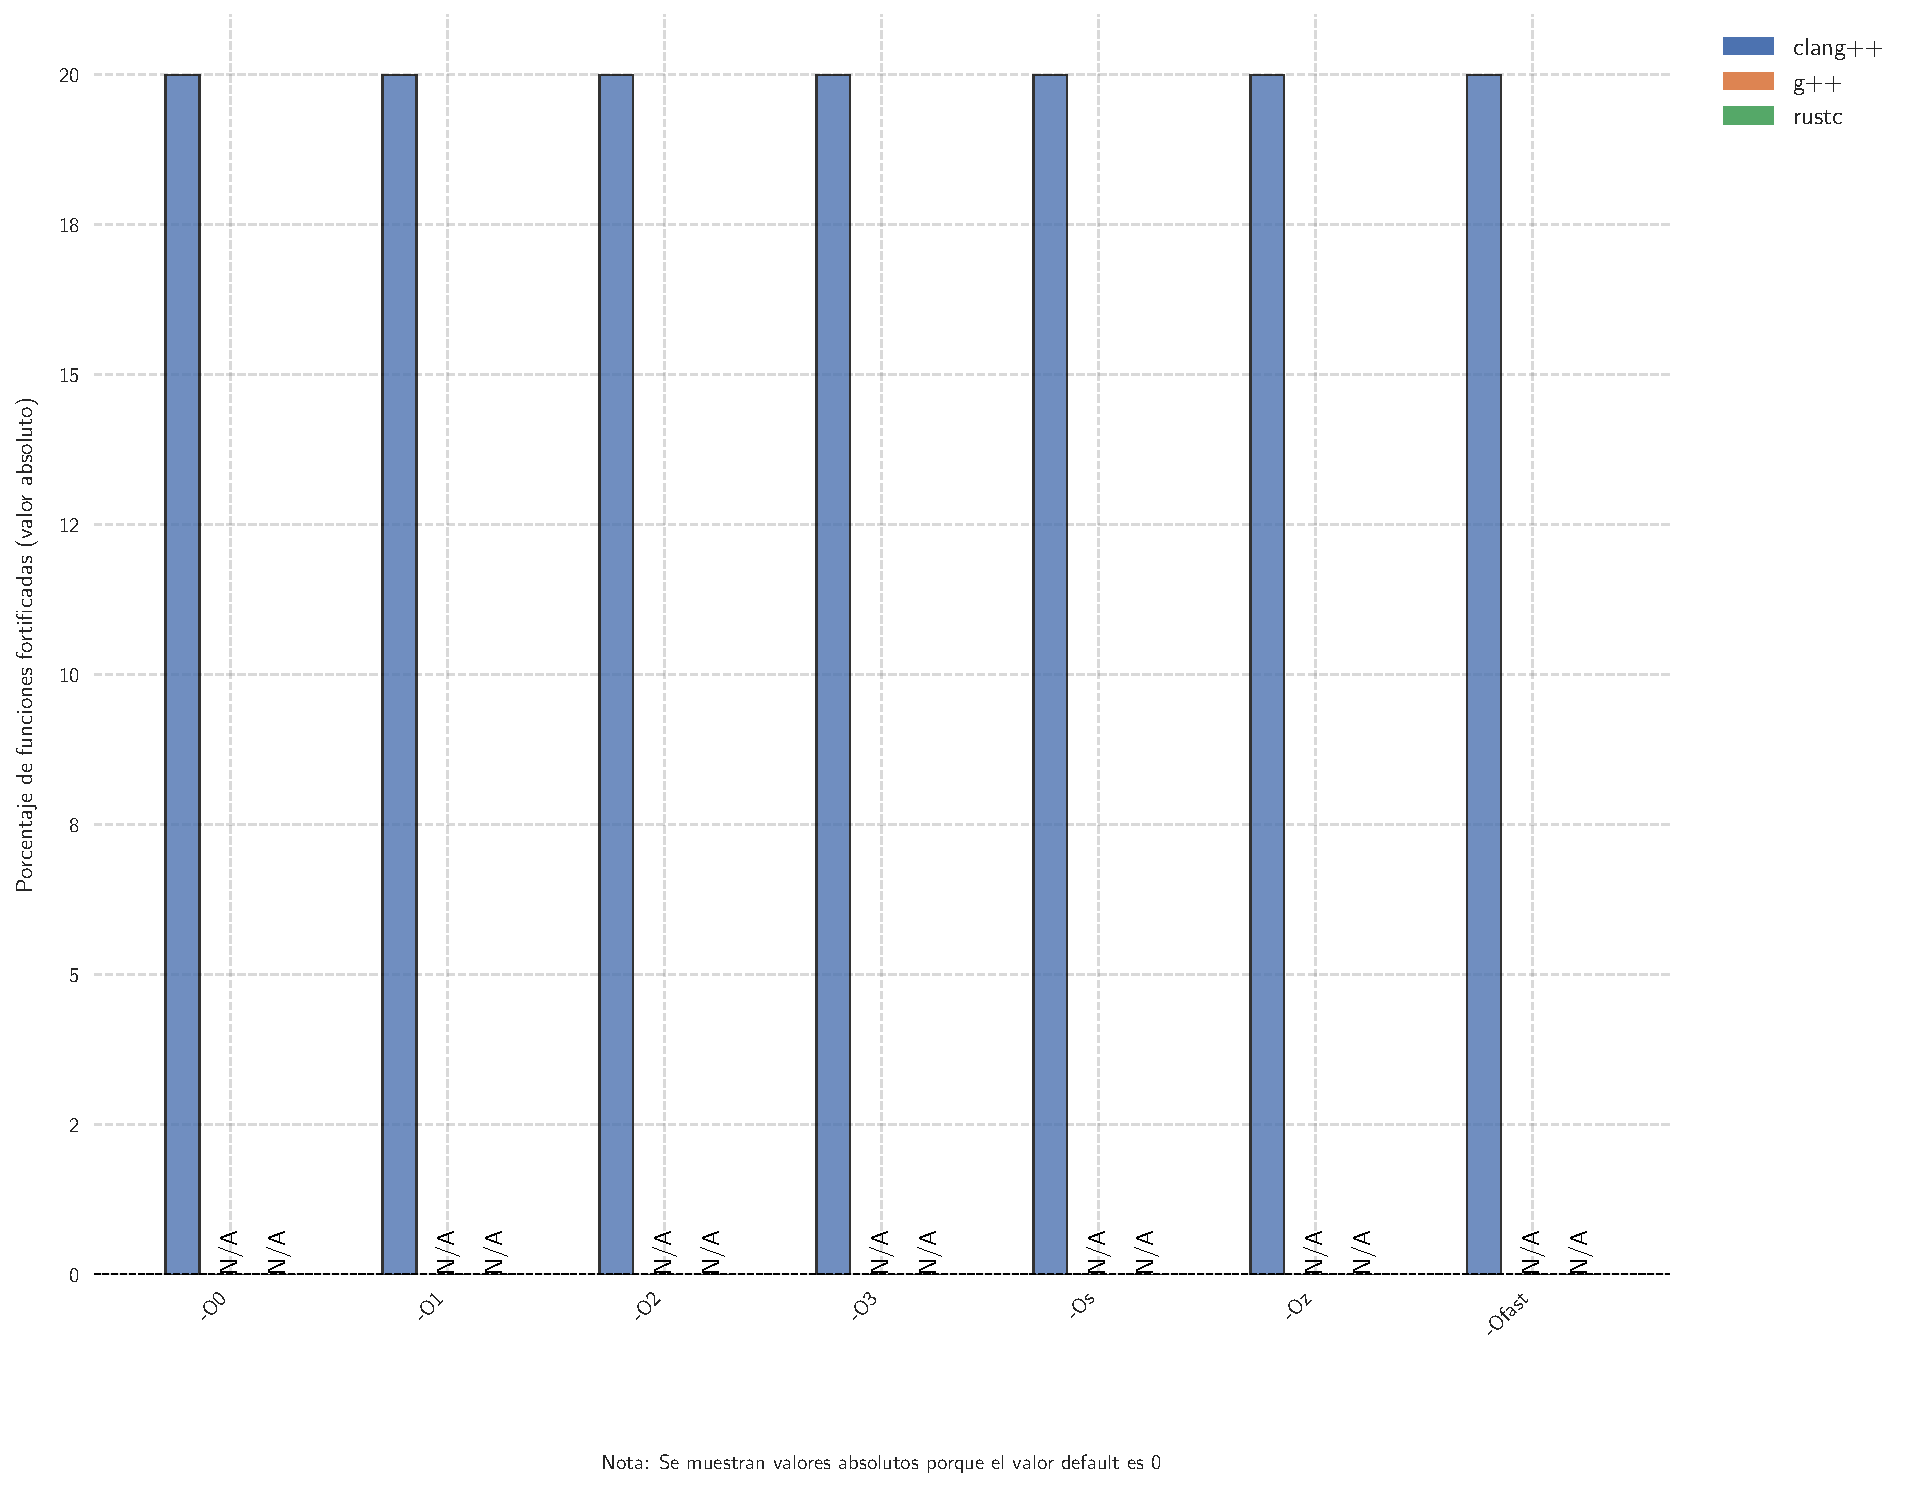
\includegraphics[width=\linewidth]{Gráficas/Gráficas_por_medida_seguridad_porcentual/safe-stack/Fortified_Functions_porcentaje.pdf}
      \label{fig:Gráficas_gráficas_por_medida_seguridad_porcentual_safe_stack_fortified_functions_porcentaje}
    }
  \end{minipage}


  \vspace{1cm}

  \begin{minipage}{0.48\textwidth}
    \centering
    \subfloat[Uso de memoria (KB) Porcentaje]{
      
\includegraphics[width=\linewidth]{Gráficas/Gráficas_por_medida_seguridad_porcentual/safe-stack/Memory_usage_KB_porcentaje.pdf}
      \label{fig:Gráficas_gráficas_por_medida_seguridad_porcentual_safe_stack_memory_usage_kb_porcentaje}
    }
  \end{minipage}
  \hfill
  \begin{minipage}{0.48\textwidth}
    \centering
    \subfloat[Tiempo (ms) Porcentaje]{
      
\includegraphics[width=\linewidth]{Gráficas/Gráficas_por_medida_seguridad_porcentual/safe-stack/Time_ms_porcentaje.pdf}
      \label{fig:Gráficas_gráficas_por_medida_seguridad_porcentual_safe_stack_time_ms_porcentaje}
    }
  \end{minipage}

\end{figure}
\newpage

% === Gráficas_por_medida_seguridad_porcentual/sanitizers/address ===
\subsection*{Sanitizadores / AddressSanitizer}
\begin{figure}[htbp]
  \centering
  \caption{Resultados para Sanitizadores (AddressSanitizer)}
  \vspace{0.5cm}

  \begin{minipage}{0.48\textwidth}
    \centering
    \subfloat[Tamaño del archivo (KB) Porcentaje]{
      
\includegraphics[width=\linewidth]{Gráficas/Gráficas_por_medida_seguridad_porcentual/sanitizers/address/File_size_KB_porcentaje.pdf}
      \label{fig:Gráficas_gráficas_por_medida_seguridad_porcentual_sanitizers_address_file_size_kb_porcentaje}
    }
  \end{minipage}
  \hfill
  \begin{minipage}{0.48\textwidth}
    \centering
    \subfloat[Funciones fortificadas (\%) Porcentaje]{
      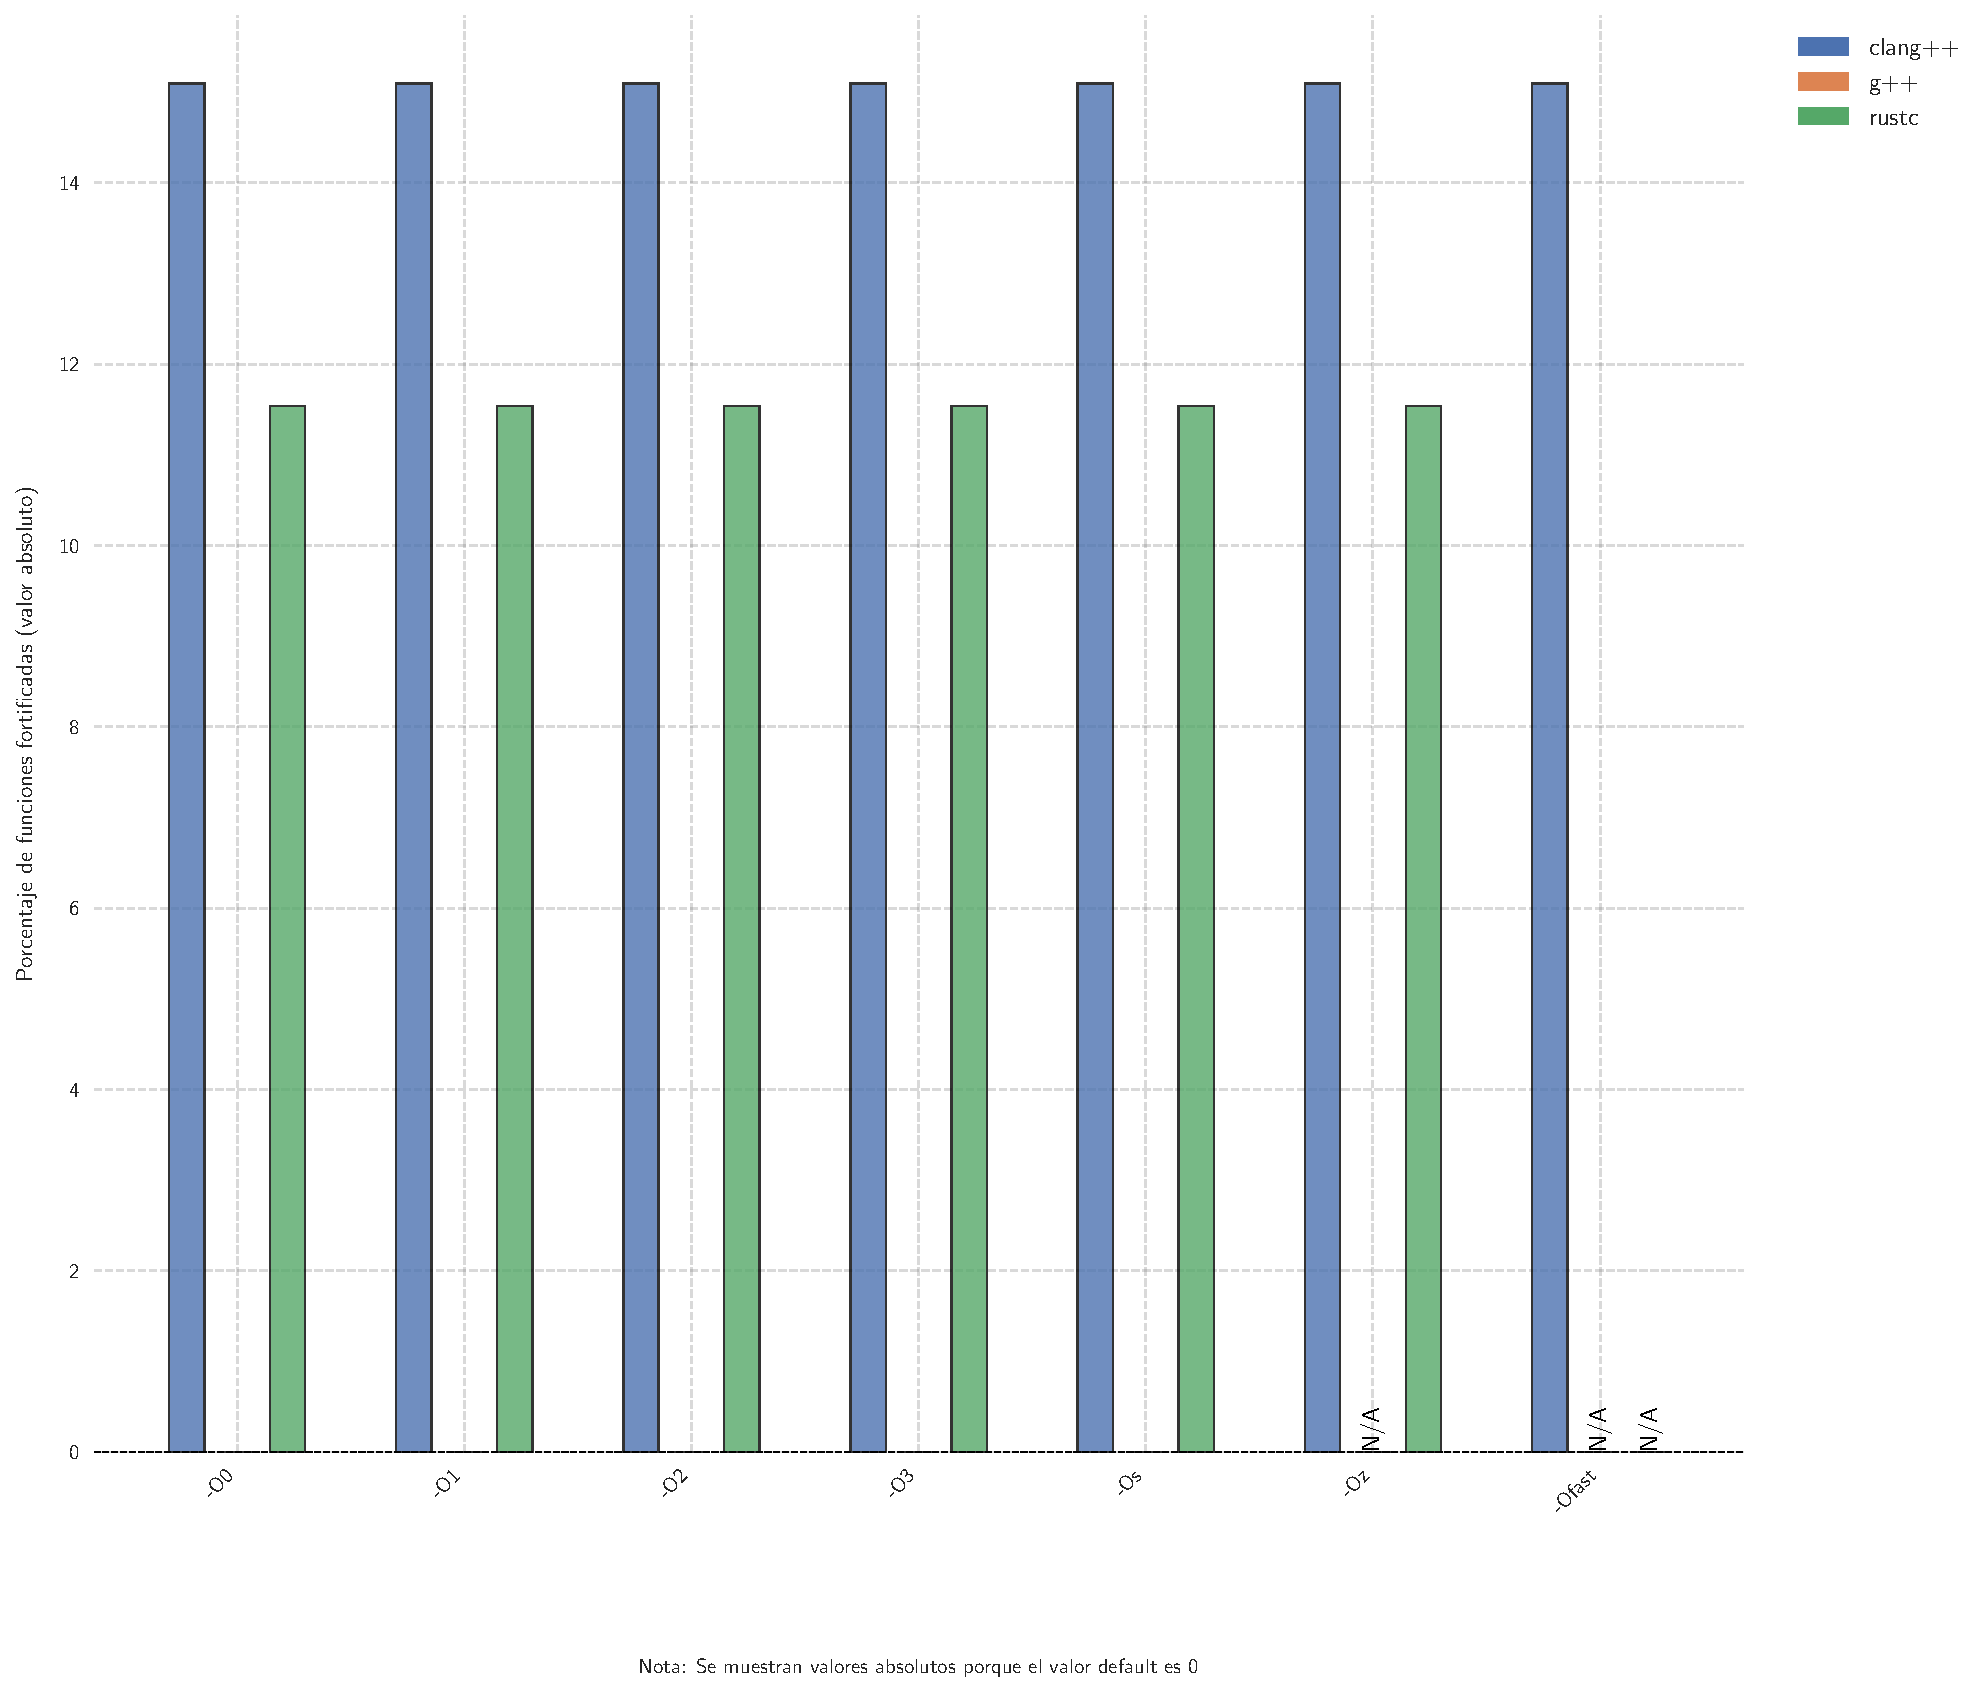
\includegraphics[width=\linewidth]{Gráficas/Gráficas_por_medida_seguridad_porcentual/sanitizers/address/Fortified_Functions_porcentaje.pdf}
      \label{fig:Gráficas_gráficas_por_medida_seguridad_porcentual_sanitizers_address_fortified_functions_porcentaje}
    }
  \end{minipage}


  \vspace{1cm}

  \begin{minipage}{0.48\textwidth}
    \centering
    \subfloat[Uso de memoria (KB) Porcentaje]{
      
\includegraphics[width=\linewidth]{Gráficas/Gráficas_por_medida_seguridad_porcentual/sanitizers/address/Memory_usage_KB_porcentaje.pdf}
      \label{fig:Gráficas_gráficas_por_medida_seguridad_porcentual_sanitizers_address_memory_usage_kb_porcentaje}
    }
  \end{minipage}
  \hfill
  \begin{minipage}{0.48\textwidth}
    \centering
    \subfloat[Tiempo (ms) Porcentaje]{
      
\includegraphics[width=\linewidth]{Gráficas/Gráficas_por_medida_seguridad_porcentual/sanitizers/address/Time_ms_porcentaje.pdf}
      \label{fig:Gráficas_gráficas_por_medida_seguridad_porcentual_sanitizers_address_time_ms_porcentaje}
    }
  \end{minipage}

\end{figure}
\newpage

% === Gráficas_por_medida_seguridad_porcentual/sanitizers/undefined ===
\subsection*{Sanitizadores / UndefinedSanitizer}
\begin{figure}[htbp]
  \centering
  \caption{Resultados para Sanitizadores (UndefinedSanitizer)}
  \vspace{0.5cm}

  \begin{minipage}{0.48\textwidth}
    \centering
    \subfloat[Tamaño del archivo (KB) Porcentaje]{
      
\includegraphics[width=\linewidth]{Gráficas/Gráficas_por_medida_seguridad_porcentual/sanitizers/undefined/File_size_KB_porcentaje.pdf}
      \label{fig:Gráficas_gráficas_por_medida_seguridad_porcentual_sanitizers_undefined_file_size_kb_porcentaje}
    }
  \end{minipage}
  \hfill
  \begin{minipage}{0.48\textwidth}
    \centering
    \subfloat[Funciones fortificadas (\%) Porcentaje]{
      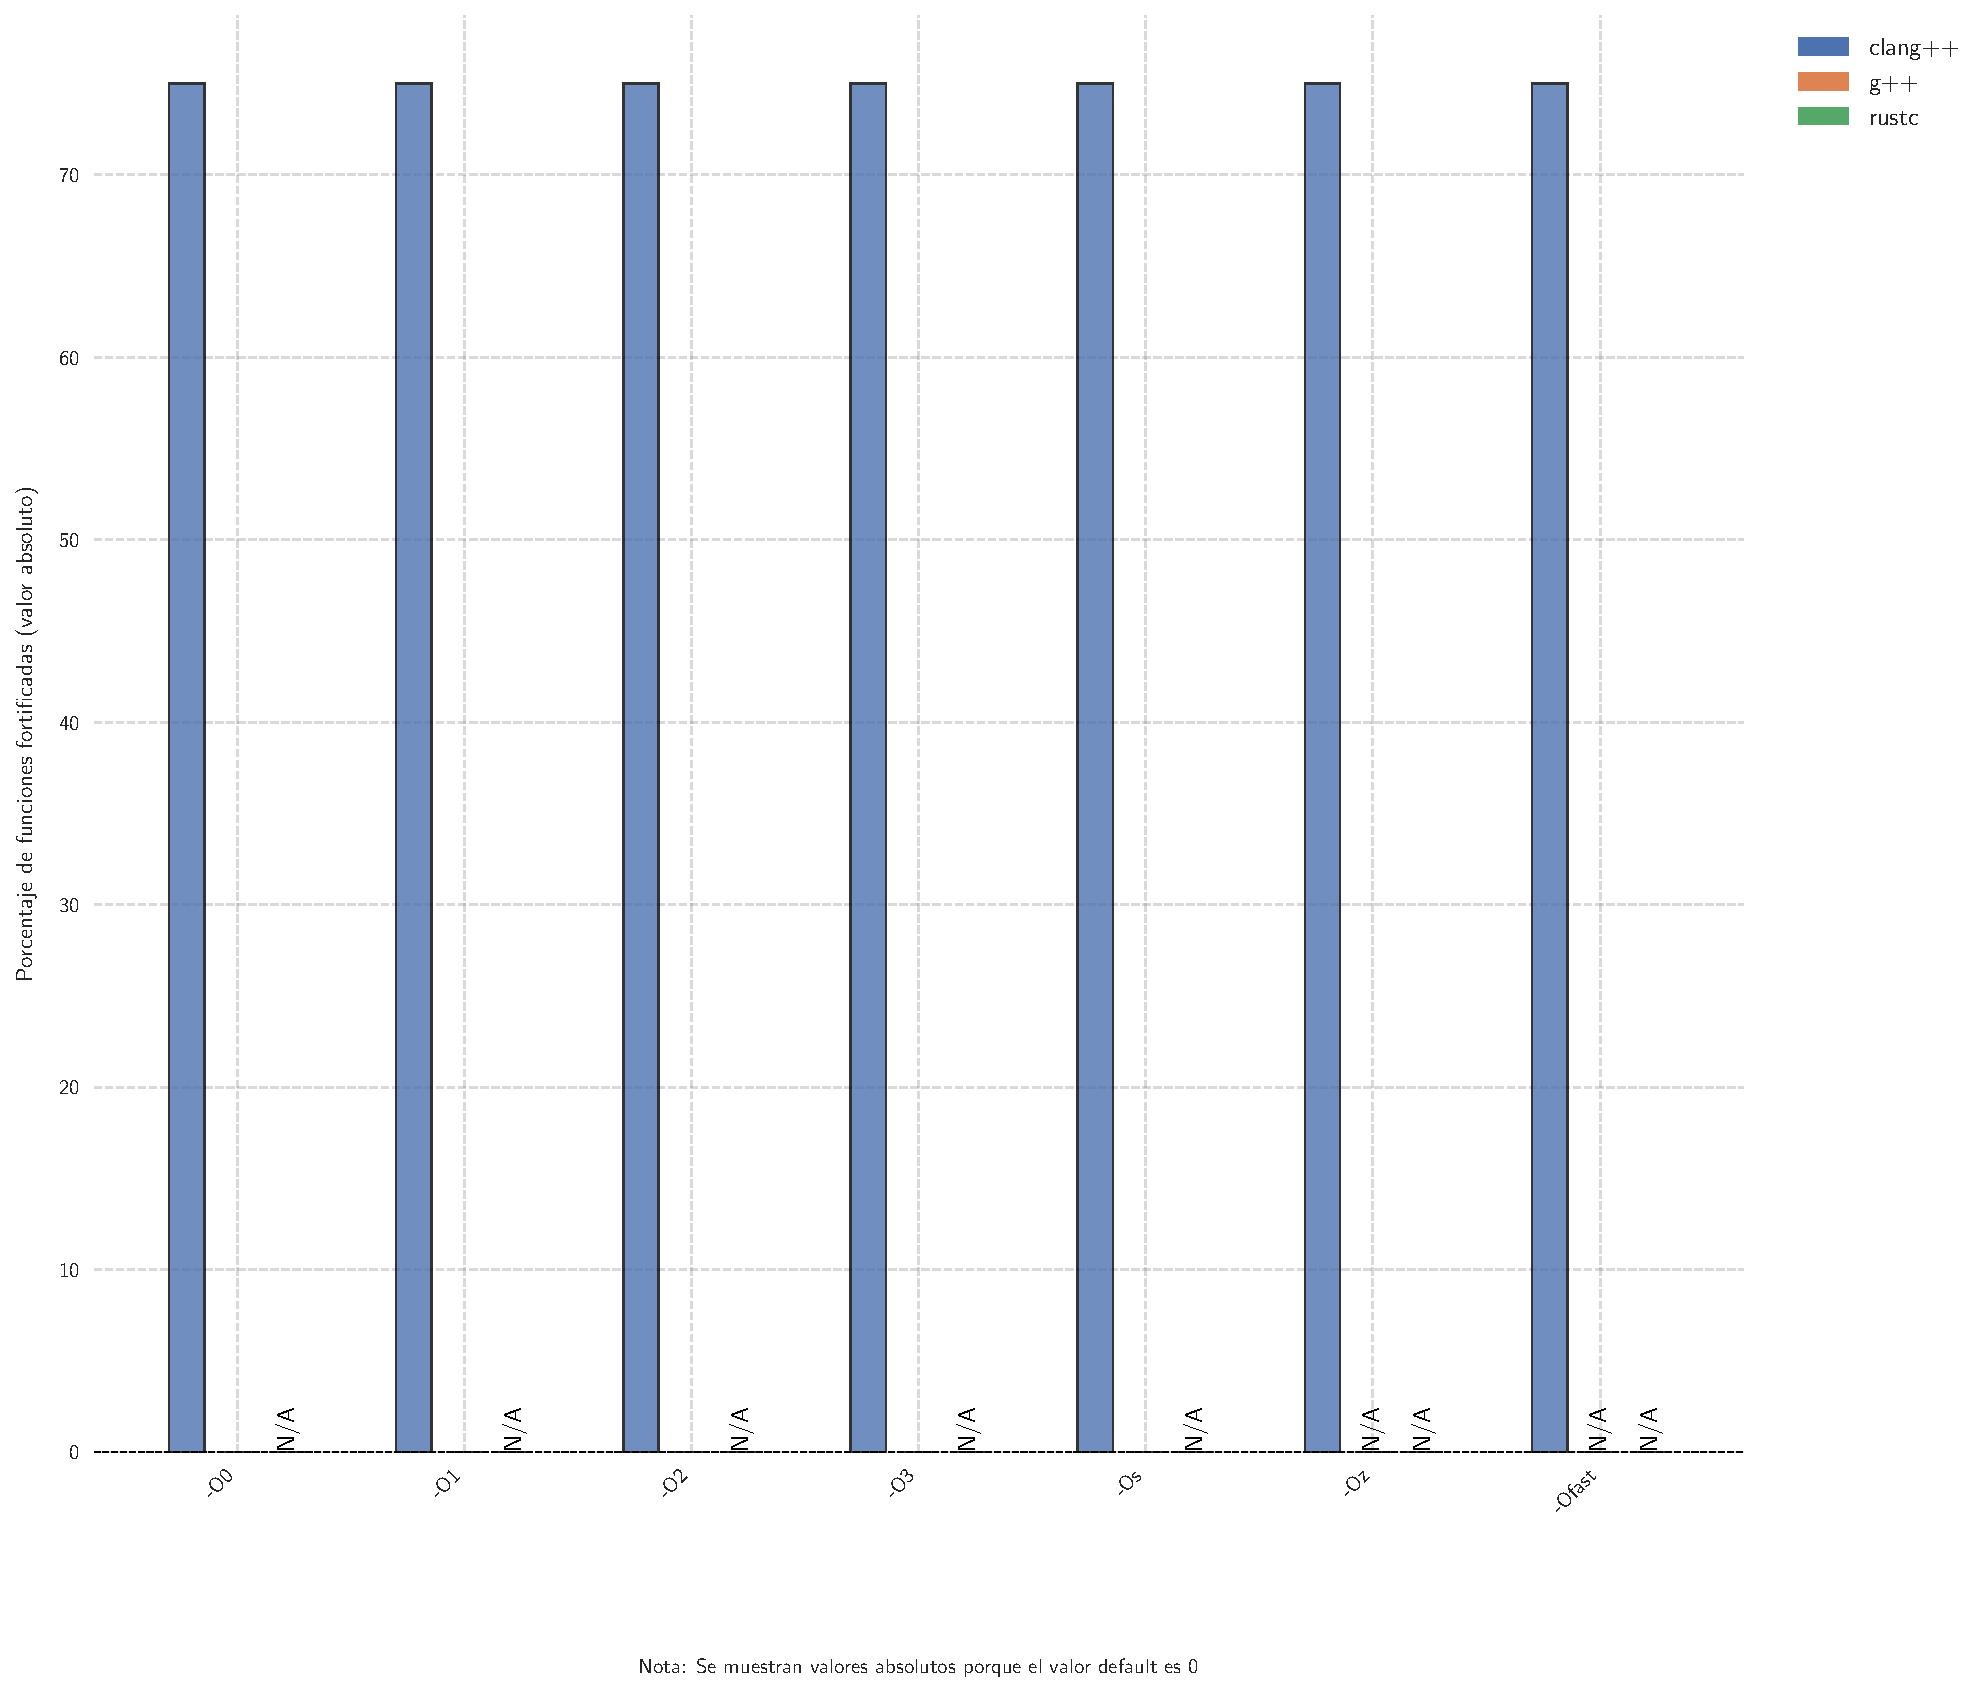
\includegraphics[width=\linewidth]{Gráficas/Gráficas_por_medida_seguridad_porcentual/sanitizers/undefined/Fortified_Functions_porcentaje.pdf}
      \label{fig:Gráficas_gráficas_por_medida_seguridad_porcentual_sanitizers_undefined_fortified_functions_porcentaje}
    }
  \end{minipage}


  \vspace{1cm}

  \begin{minipage}{0.48\textwidth}
    \centering
    \subfloat[Uso de memoria (KB) Porcentaje]{
      
\includegraphics[width=\linewidth]{Gráficas/Gráficas_por_medida_seguridad_porcentual/sanitizers/undefined/Memory_usage_KB_porcentaje.pdf}
      \label{fig:Gráficas_gráficas_por_medida_seguridad_porcentual_sanitizers_undefined_memory_usage_kb_porcentaje}
    }
  \end{minipage}
  \hfill
  \begin{minipage}{0.48\textwidth}
    \centering
    \subfloat[Tiempo (ms) Porcentaje]{
      
\includegraphics[width=\linewidth]{Gráficas/Gráficas_por_medida_seguridad_porcentual/sanitizers/undefined/Time_ms_porcentaje.pdf}
      \label{fig:Gráficas_gráficas_por_medida_seguridad_porcentual_sanitizers_undefined_time_ms_porcentaje}
    }
  \end{minipage}

\end{figure}
\newpage

% === Gráficas_por_medida_seguridad_porcentual/stack-protection/all ===
\subsection*{Stack protector / all}
\begin{figure}[htbp]
  \centering
  \caption{Resultados para Stack protector (all)}
  \vspace{0.5cm}

  \begin{minipage}{0.48\textwidth}
    \centering
    \subfloat[Tamaño del archivo (KB) Porcentaje]{
      
\includegraphics[width=\linewidth]{Gráficas/Gráficas_por_medida_seguridad_porcentual/stack-protection/all/File_size_KB_porcentaje.pdf}
      \label{fig:Gráficas_gráficas_por_medida_seguridad_porcentual_stack_protection_all_file_size_kb_porcentaje}
    }
  \end{minipage}
  \hfill
  \begin{minipage}{0.48\textwidth}
    \centering
    \subfloat[Funciones fortificadas (\%) Porcentaje]{
      \includegraphics[width=\linewidth]{Gráficas/Gráficas_por_medida_seguridad_porcentual/stack-protection/all/Fortified_Functions_porcentaje.pdf}
      \label{fig:Gráficas_gráficas_por_medida_seguridad_porcentual_stack_protection_all_fortified_functions_porcentaje}
    }
  \end{minipage}


  \vspace{1cm}

  \begin{minipage}{0.48\textwidth}
    \centering
    \subfloat[Uso de memoria (KB) Porcentaje]{
      
\includegraphics[width=\linewidth]{Gráficas/Gráficas_por_medida_seguridad_porcentual/stack-protection/all/Memory_usage_KB_porcentaje.pdf}
      \label{fig:Gráficas_gráficas_por_medida_seguridad_porcentual_stack_protection_all_memory_usage_kb_porcentaje}
    }
  \end{minipage}
  \hfill
  \begin{minipage}{0.48\textwidth}
    \centering
    \subfloat[Tiempo (ms) Porcentaje]{
      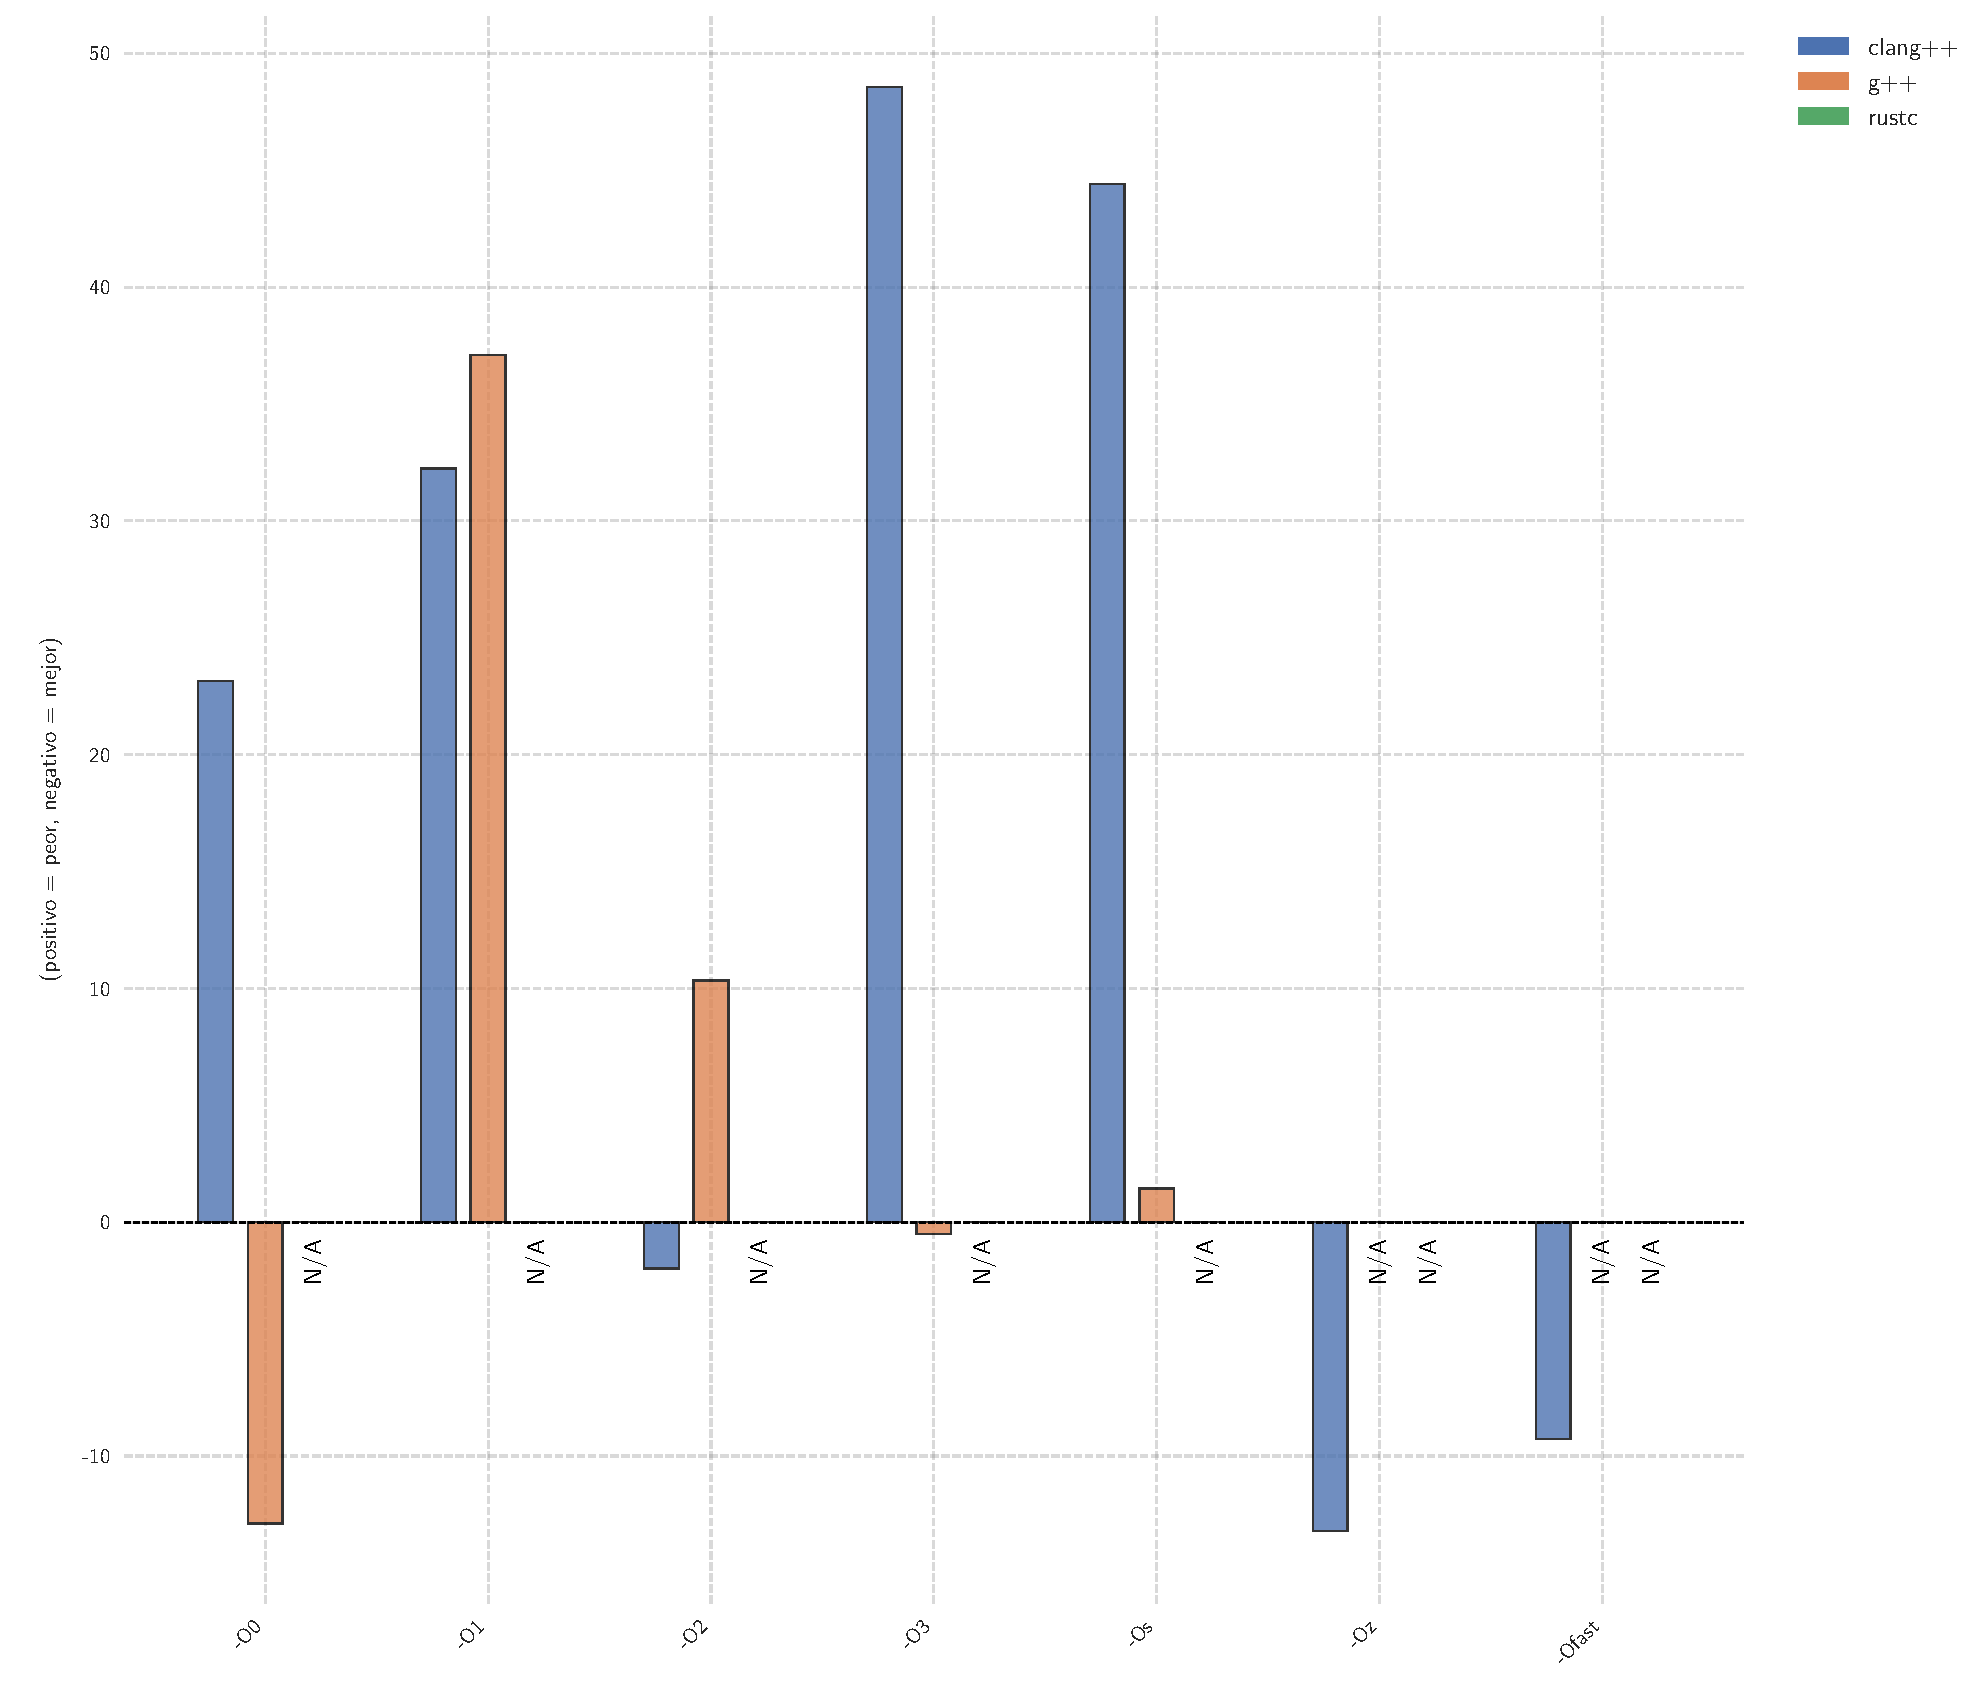
\includegraphics[width=\linewidth]{Gráficas/Gráficas_por_medida_seguridad_porcentual/stack-protection/all/Time_ms_porcentaje.pdf}
      \label{fig:Gráficas_gráficas_por_medida_seguridad_porcentual_stack_protection_all_time_ms_porcentaje}
    }
  \end{minipage}

\end{figure}
\newpage

% === Gráficas_por_medida_seguridad_porcentual/stack-protection/basic ===
\subsection*{Stack protector / basic}
\begin{figure}[htbp]
  \centering
  \caption{Resultados para Stack protector (basic)}
  \vspace{0.5cm}

  \begin{minipage}{0.48\textwidth}
    \centering
    \subfloat[Tamaño del archivo (KB) Porcentaje]{
      
\includegraphics[width=\linewidth]{Gráficas/Gráficas_por_medida_seguridad_porcentual/stack-protection/basic/File_size_KB_porcentaje.pdf}
      \label{fig:Gráficas_gráficas_por_medida_seguridad_porcentual_stack_protection_basic_file_size_kb_porcentaje}
    }
  \end{minipage}
  \hfill
  \begin{minipage}{0.48\textwidth}
    \centering
    \subfloat[Funciones fortificadas (\%) Porcentaje]{
      \includegraphics[width=\linewidth]{Gráficas/Gráficas_por_medida_seguridad_porcentual/stack-protection/basic/Fortified_Functions_porcentaje.pdf}
      \label{fig:Gráficas_gráficas_por_medida_seguridad_porcentual_stack_protection_basic_fortified_functions_porcentaje}
    }
  \end{minipage}


  \vspace{1cm}

  \begin{minipage}{0.48\textwidth}
    \centering
    \subfloat[Uso de memoria (KB) Porcentaje]{
      
\includegraphics[width=\linewidth]{Gráficas/Gráficas_por_medida_seguridad_porcentual/stack-protection/basic/Memory_usage_KB_porcentaje.pdf}
      \label{fig:Gráficas_gráficas_por_medida_seguridad_porcentual_stack_protection_basic_memory_usage_kb_porcentaje}
    }
  \end{minipage}
  \hfill
  \begin{minipage}{0.48\textwidth}
    \centering
    \subfloat[Tiempo (ms) Porcentaje]{
      
\includegraphics[width=\linewidth]{Gráficas/Gráficas_por_medida_seguridad_porcentual/stack-protection/basic/Time_ms_porcentaje.pdf}
      \label{fig:Gráficas_gráficas_por_medida_seguridad_porcentual_stack_protection_basic_time_ms_porcentaje}
    }
  \end{minipage}

\end{figure}
\newpage

% === Gráficas_por_medida_seguridad_porcentual/stack-protection/disabled ===
\subsection*{Stack protector / disabled}
\begin{figure}[htbp]
  \centering
  \caption{Resultados para Stack protector (disabled)}
  \vspace{0.5cm}

  \begin{minipage}{0.48\textwidth}
    \centering
    \subfloat[Tamaño del archivo (KB) Porcentaje]{
      
\includegraphics[width=\linewidth]{Gráficas/Gráficas_por_medida_seguridad_porcentual/stack-protection/disabled/File_size_KB_porcentaje.pdf}
      \label{fig:Gráficas_gráficas_por_medida_seguridad_porcentual_stack_protection_disabled_file_size_kb_porcentaje}
    }
  \end{minipage}
  \hfill
  \begin{minipage}{0.48\textwidth}
    \centering
    \subfloat[Funciones fortificadas (\%) Porcentaje]{
      \includegraphics[width=\linewidth]{Gráficas/Gráficas_por_medida_seguridad_porcentual/stack-protection/disabled/Fortified_Functions_porcentaje.pdf}
      \label{fig:Gráficas_gráficas_por_medida_seguridad_porcentual_stack_protection_disabled_fortified_functions_porcentaje}
    }
  \end{minipage}


  \vspace{1cm}

  \begin{minipage}{0.48\textwidth}
    \centering
    \subfloat[Uso de memoria (KB) Porcentaje]{
      \includegraphics[width=\linewidth]{Gráficas/Gráficas_por_medida_seguridad_porcentual/stack-protection/disabled/Memory_usage_KB_porcentaje.pdf}
      \label{fig:Gráficas_gráficas_por_medida_seguridad_porcentual_stack_protection_disabled_memory_usage_kb_porcentaje}
    }
  \end{minipage}
  \hfill
  \begin{minipage}{0.48\textwidth}
    \centering
    \subfloat[Tiempo (ms) Porcentaje]{
      \includegraphics[width=\linewidth]{Gráficas/Gráficas_por_medida_seguridad_porcentual/stack-protection/disabled/Time_ms_porcentaje.pdf}
      \label{fig:Gráficas_gráficas_por_medida_seguridad_porcentual_stack_protection_disabled_time_ms_porcentaje}
    }
  \end{minipage}

\end{figure}
\newpage

% === Gráficas_por_medida_seguridad_porcentual/stack-protection/strong ===
\subsection*{Stack protector / strong}
\begin{figure}[htbp]
  \centering
  \caption{Resultados para Stack protector (strong)}
  \vspace{0.5cm}

  \begin{minipage}{0.48\textwidth}
    \centering
    \subfloat[Tamaño del archivo (KB) Porcentaje]{
      \includegraphics[width=\linewidth]{Gráficas/Gráficas_por_medida_seguridad_porcentual/stack-protection/strong/File_size_KB_porcentaje.pdf}
      \label{fig:Gráficas_gráficas_por_medida_seguridad_porcentual_stack_protection_strong_file_size_kb_porcentaje}
    }
  \end{minipage}
  \hfill
  \begin{minipage}{0.48\textwidth}
    \centering
    \subfloat[Funciones fortificadas (\%) Porcentaje]{
      \includegraphics[width=\linewidth]{Gráficas/Gráficas_por_medida_seguridad_porcentual/stack-protection/strong/Fortified_Functions_porcentaje.pdf}
      \label{fig:Gráficas_gráficas_por_medida_seguridad_porcentual_stack_protection_strong_fortified_functions_porcentaje}
    }
  \end{minipage}


  \vspace{1cm}

  \begin{minipage}{0.48\textwidth}
    \centering
    \subfloat[Uso de memoria (KB) Porcentaje]{
      \includegraphics[width=\linewidth]{Gráficas/Gráficas_por_medida_seguridad_porcentual/stack-protection/strong/Memory_usage_KB_porcentaje.pdf}
      \label{fig:Gráficas_gráficas_por_medida_seguridad_porcentual_stack_protection_strong_memory_usage_kb_porcentaje}
    }
  \end{minipage}
  \hfill
  \begin{minipage}{0.48\textwidth}
    \centering
    \subfloat[Tiempo (ms) Porcentaje]{
      \includegraphics[width=\linewidth]{Gráficas/Gráficas_por_medida_seguridad_porcentual/stack-protection/strong/Time_ms_porcentaje.pdf}
      \label{fig:Gráficas_gráficas_por_medida_seguridad_porcentual_stack_protection_strong_time_ms_porcentaje}
    }
  \end{minipage}

\end{figure}
\newpage

\end{document}
